%% DOCUMENT CLASS (alternative to book is 'report')
% Print just right page or both sides (comment the other one)
%\documentclass[12pt,a4paper,openright,oneside]{book}	%%One sided
\documentclass[12pt,a4paper,openright,twoside]{book}	%%Double sided

%% SET MARGINS OF THE PAGES
\usepackage{geometry}
\geometry{a4paper,portrait, left=35mm, right=20mm, top=35mm, bottom=30mm}

%% HEADERS AND FOOTERS
\usepackage{fancyhdr}
\pagestyle{fancy}
\fancyhf{} 			%clears default header and footer
\rhead{} 			%right head
\lhead{ \leftmark} 	%left head
\rfoot{\thepage}
%%consider using also chead, cfoot, lfoot
%coherce the plain stile to this (e.g. the first page of every chapter)
\fancypagestyle{plain}{
	\fancyhf{}
	\rfoot{\thepage}
	\renewcommand{\headrulewidth}{0pt}
	\renewcommand{\footrulewidth}{0pt}
}
\setlength{\headheight}{15pt}
%% CLEAR PAGE WITHOUT NUMBER AT THE BEGINNING OF CHAPTERS
\let\origdoublepage\cleardoublepage
\newcommand{\clearemptydoublepage}{%
  \clearpage
  {\pagestyle{empty}\origdoublepage}%
}
%% CMS COMMANDS (slightly modified since I could not fix some ifthenelse with booleans)
\usepackage{ptdr-definitions}
\usepackage{heppennames2}
% CUSTOM COMMANDS
\newcommand{\todo}[1]{\textcolor{red}{[TODO: #1]}}
\newcommand{\note}[1]{\textcolor{blue}{[NOTE: #1]}}
\newcommand{\usep}{\nobreak\hspace{.16667em plus .08333em}}
\newcommand{\Lagrangian}{\mathcal{L}}
\newcommand{\Likelihood}{\mathcal{L}}
\newcommand{\Probability}{p}%{\mathbb{P}}
\newcommand{\Celsius}{\ensuremath{\usep ^{\circ}\mathrm{C}}\xspace}
\newcommand{\mathdefined}{\ensuremath{\stackrel{\text{\tiny def}}{=}}}
\newcommand{\SIPthreeD}{\ensuremath{\mathrm{SIP}_{\mathrm{3D}}}\xspace}
\newcommand{\sieie}{\ensuremath{\sigma_{i \eta i \eta}}\xspace}
\newcommand{\nonprompt}{non-prompt\xspace}
\newcommand{\Nonprompt}{Non-prompt\xspace}
\newcommand{\Pileup}{Pileup}
\newcommand{\pileup}{pileup}
\newcommand{\antikt}{\mbox{\text{anti-}\ensuremath{k_t}}\xspace}
\newcommand{\ins}{\ensuremath{\,\in\,}} % \in with spaces around
\renewcommand{\mum}{\ensuremath{\,}\text{{\textmu}m}\xspace}
\newcommand{\Run}[1]{Run\nobreak\hspace{.22222em plus .11111em}#1}
\newcommand{\RunII}{\Run{2}}
\newcommand{\MADSPIN}{{\textsc{MadSpin}}\xspace}

%% Overwrite some definitions
%% Note: \DeclareRobustCommand does not check for previous definitions
\DeclareRobustCommand{\Pl}{{\HepParticle{\mathrm{\ell}}{}{}}\Xspace} % lepton
\DeclareRobustCommand{\PGnl}{{\HepParticle{\PGn}{\mathrm{\ell}}{}}\Xspace} % neutrino (for lepton l)
\DeclareRobustCommand{\PAGnl}{{\HepAntiParticle{\PGn}{\mathrm{\ell}}{}}\Xspace} % anti-neutrino (for lepton l)

%% Switches
\newcommand{\expobs}{expected}   % {expected}: blind results, {observed}: unblind results
\newcommand{\dataMCblind}{_blind}% {blind}   : blind results, {}        : unblind results

%% ALLOW PAGE ROTATION
\usepackage{lscape}

%% HYPERTEXT SETUP
\usepackage{hyperref}
\hypersetup{
    colorlinks,
    citecolor=black,
    filecolor=black,
    linkcolor=black,
    urlcolor=black
}
%% PDF SETTINGS
\hypersetup{
    pdfauthor={Alberto Mecca},
    pdftitle={Triboson Production ZZG},
    pdfsubject={},
    pdfkeywords={
      CMS,
      Particle data analysis,
      Electroweak interaction,
      W and Z bosons,
      Leptons,
      Photons
    }
}
%% FONTS AND SYMBOLS
\usepackage[utf8]{inputenc}	%%input font setting
\usepackage[T1]{fontenc} 		%%font for automatic recognition of letters with the accent
\usepackage{amsfonts}		%%fonts for the mathematical rendering of formulas
\usepackage{amssymb}
\usepackage{amsmath}
\usepackage{slashed}
%% CHAPTERS STRUCTURE
\usepackage[italian,british]{babel} %%Set English as main language of the document
\usepackage{appendix}
\setcounter{tocdepth}{3}
\setcounter{secnumdepth}{3}
%% FIGURES
\usepackage{graphicx}
\usepackage{subfigure}		%%allow side by side figures with single caption
\usepackage{rotating}           %%sidewaystable and friends
%% TABLES
\usepackage{multirow}		%%allow to merge rows in the tables
\usepackage{booktabs}		%%allow use of \toprule, \midrule, \bottomrule in tables
\usepackage{array}
\usepackage[table]{xcolor}      %%background color of individual cells
\usepackage{makecell}           %%saner way to define multiline cells
%%CAPTIONS
\usepackage[font=small, labelfont=bf]{caption}
%% BIBLIOGRAPHY
\usepackage[babel]{csquotes}
\usepackage[sorting=none, backend=biber, style=numeric-comp]{biblatex}
\addbibresource{bibliography/thesis.bib}
\addbibresource{bibliography/CMS_publications_pub.bib}
%% CODE LISTINGS
\usepackage{listings}		%%allow to use code listings
%% PROVIDE \thetitle, \theauthor and \thedate
\usepackage{titling}
\author{Alberto Mecca}
\title{Triboson production in the $VZ\gamma$ channel in proton-proton collisions with the CMS experiment at 13 TeV}

%% HYPENATON
\hyphenation{te-si ATLAS}	%manual hyphenation
%% STYLE
\linespread{1.1}
\renewcommand{\arraystretch}{1.1}
%% FIGURES FOLDER
\graphicspath{{.}{Figures}{Figures/Feynman}{Figures/combine}}


%%%%%%%%%%%%%%%%%%%%%%%%%%%%%%%%%%%%%%%%%%%%%%%%%
%%%% BEGIN DOCUMENT
\begin{document}

%%%%%% HEAD  OF THE DOCUMENT
\frontmatter
%%FRONT PAGE
%%%%%%%%%%%%%%%%%%%%%%%%%%%%%%%%%%%%%%%%%%%%%%%%%%%%%%%%%%
\begin{titlepage}

%\thispagestyle{empty}
\pagenumbering{arabic}
\begin{center}
\begin{large}
Universit\`a degli Studi di Torino \\
{\bf Scuola~di~Dottorato}
\end{large}
\end{center}
\hrulefill

\vspace{-0.5cm}
\begin{figure}[h]
  \centering
  
\includegraphics[width=.8\textwidth]{pictures/LogoUnito_Orizzontale_Colore_resize30percent.png}
\end{figure}

\vspace{-1cm}
\begin{center}
\begin{Large}
{\bf Tesi di Dottorato in Fisica}
\end{Large}
\end{center}

\vspace{2cm}
\LARGE{\bf Titolo titolo titolo titolo titolo titolo titolo}

\vspace*{\fill}
\large{\bf Candidate: Alberto Mecca}

\vspace{1cm}
\large{\bf Supervisor: Prof. Riccardo Bellan}

\end{titlepage}

\clearemptydoublepage
%%DEDICATION (the initial quote)
\thispagestyle{empty}
\begin{flushright}

\vspace*{60mm}

\begin{quote}
The last ever dolphin message was misinterpreted as a surprisingly sophisticated attempt to do a double-backwards-somersault through a hoop whilst whistling the 'Star Spangled Banner', but in fact the message was this: \mbox{So long and thanks for all the fish.}
%For instance, on the planet Earth, man had always assumed that he was more intelligent than dolphins because he had achieved so much --- the wheel, New York, wars and so on --- whilst all the dolphins had ever done was muck about in the water having a good time. But conversely, the dolphins had always believed that they were far more intelligent than man --- for precisely the same reasons.
% I'd far rather be happy than right any day.
% We demand rigidly defined areas of doubt and uncertainty!
\end{quote}
\vspace{4mm}
Douglas Adams, \textit{The Hitchhiker's Guide to the Galaxy}

\end{flushright}

\clearemptydoublepage
%%ABSTRACT
\chapter*{Abstract}

Here goes the abstract: This thesis will cover a brief introduction of lattice gauge theories and how they are still actively used in investigating confinement in QCD. Within this framework I will also mention the link between lattice gauge theories and spin systems.
The main topic of this thesis is the investigation using lattice QCD of inclusive semileptonic decays of heavy meson. I will start by discussing what lattice QCD is and the sate of the art simulation for Twisted Mass fermions (and Domain Wall fermions). Then I will present the main challenge of this type of calculations, namely solving the ill-posed inverse problem which is required for the inclusive calculation. we will certainly cite this work: \cite{Gambino:2022dvu}

Vestibulum quis vehicula massa. Etiam dictum, enim vel luctus accumsan, dolor velit laoreet metus, nec pretium arcu dui nec nulla. Donec ac sollicitudin justo, ut ullamcorper nunc. Curabitur ornare, ipsum hendrerit dictum rutrum, nisl lectus cursus sapien, in condimentum ipsum magna vel lorem. Cras vulputate semper placerat. In nec quam condimentum, auctor nisl eu, viverra libero. Maecenas scelerisque, odio vel accumsan luctus, justo dui pharetra orci, sit amet feugiat lorem lacus ac enim. Donec ultrices nulla semper erat consectetur, vitae mattis nulla dictum. Fusce maximus tristique condimentum. Quisque et sodales lectus, vel posuere leo. In ac augue vel neque sagittis volutpat at nec justo. Proin bibendum lobortis neque, vitae vulputate lorem viverra in. Etiam neque risus, pretium sed tempor a, pharetra quis arcu. Morbi purus nibh, efficitur nec sollicitudin non, commodo vel massa.

Pellentesque eu neque lacus. Vivamus finibus consectetur tellus id imperdiet. In ut dolor ligula. Vivamus ac vehicula erat. Duis semper lacinia eros, sed ultrices orci tristique at. Proin in pellentesque massa. Nunc ultricies justo eget nibh condimentum sollicitudin. Mauris non ligula eget magna pulvinar pretium vel vitae ante. Aenean lacinia metus vel odio vehicula sollicitudin. Quisque nisi augue, faucibus a nulla faucibus, consequat vehicula elit. Donec dui mi, ornare quis sapien ac, finibus maximus mi. Etiam volutpat, arcu quis posuere sollicitudin, ligula elit tincidunt lectus, non dapibus augue nunc id est. Ut dictum et diam vel vulputate. Aliquam ut nibh eu nibh aliquet aliquam eget ut leo. Duis urna tellus, sodales non ornare ut, aliquet vitae mi. Nunc consequat est vitae elit consectetur, id iaculis libero congue.

Praesent sem neque, semper ac turpis eu, fringilla egestas erat. Fusce in leo velit. Sed faucibus viverra massa. Donec justo lorem, accumsan a nisi in, maximus placerat augue. Mauris posuere aliquet sapien sed viverra. In hac habitasse platea dictumst. Ut nec dictum purus, sit amet gravida risus.

\chapter*{Italian abstract}

Lorem ipsum dolor sit amet, consectetur adipiscing elit. Vestibulum nec augue tincidunt, sodales lorem fringilla, venenatis metus. Cras dictum nec urna vitae euismod. Nunc vulputate quam dolor, id convallis augue convallis sit amet. Aliquam nec felis sodales, condimentum massa ac, tincidunt nisi. Vestibulum posuere, lacus tempus facilisis cursus, velit libero mattis diam, vel aliquet magna turpis vitae ligula. Maecenas aliquet nulla at gravida mattis. Morbi vestibulum in ex sed ultricies. Morbi sodales mollis mauris, vitae tincidunt enim hendrerit et. Interdum et malesuada fames ac ante ipsum primis in faucibus. Suspendisse laoreet faucibus massa, quis elementum enim eleifend aliquet. Class aptent taciti sociosqu ad litora torquent per conubia nostra, per inceptos himenaeos. Etiam at tortor vestibulum, dictum augue ut, porta lorem. Sed venenatis feugiat diam. Integer eu diam nec dolor viverra hendrerit.

Vestibulum quis vehicula massa. Etiam dictum, enim vel luctus accumsan, dolor velit laoreet metus, nec pretium arcu dui nec nulla. Donec ac sollicitudin justo, ut ullamcorper nunc. Curabitur ornare, ipsum hendrerit dictum rutrum, nisl lectus cursus sapien, in condimentum ipsum magna vel lorem. Cras vulputate semper placerat. In nec quam condimentum, auctor nisl eu, viverra libero. Maecenas scelerisque, odio vel accumsan luctus, justo dui pharetra orci, sit amet feugiat lorem lacus ac enim. Donec ultrices nulla semper erat consectetur, vitae mattis nulla dictum. Fusce maximus tristique condimentum. Quisque et sodales lectus, vel posuere leo. In ac augue vel neque sagittis volutpat at nec justo. Proin bibendum lobortis neque, vitae vulputate lorem viverra in. Etiam neque risus, pretium sed tempor a, pharetra quis arcu. Morbi purus nibh, efficitur nec sollicitudin non, commodo vel massa.

Pellentesque eu neque lacus. Vivamus finibus consectetur tellus id imperdiet. In ut dolor ligula. Vivamus ac vehicula erat. Duis semper lacinia eros, sed ultrices orci tristique at. Proin in pellentesque massa. Nunc ultricies justo eget nibh condimentum sollicitudin. Mauris non ligula eget magna pulvinar pretium vel vitae ante. Aenean lacinia metus vel odio vehicula sollicitudin. Quisque nisi augue, faucibus a nulla faucibus, consequat vehicula elit. Donec dui mi, ornare quis sapien ac, finibus maximus mi. Etiam volutpat, arcu quis posuere sollicitudin, ligula elit tincidunt lectus, non dapibus augue nunc id est. Ut dictum et diam vel vulputate. Aliquam ut nibh eu nibh aliquet aliquam eget ut leo. Duis urna tellus, sodales non ornare ut, aliquet vitae mi. Nunc consequat est vitae elit consectetur, id iaculis libero congue.

Praesent sem neque, semper ac turpis eu, fringilla egestas erat. Fusce in leo velit. Sed faucibus viverra massa. Donec justo lorem, accumsan a nisi in, maximus placerat augue. Mauris posuere aliquet sapien sed viverra. In hac habitasse platea dictumst. Ut nec dictum purus, sit amet gravida risus.

\clearemptydoublepage
%%INDEXES
%summary
\tableofcontents
\clearemptydoublepage

%%%%%% BODY OF THE DOCUMENT
\mainmatter
%%INTRODUCTION
\chapter{Theoretical framework}
\section{The Standard Model of particle physics}
The Standard Model (SM) of particle physics is a renormalisable quantum field theory based on gauge invariance principles.
The underlying principle is the quantization of the elementary constituents of matter and force carriers,
as excitations of the corresponding quantum fields.
At its core, the Standard Model postulates a set of elementary particles, divided into fermions, with half-integer spin and bosons, with integer spin.
It describes three of the four known fundamental interactions: electromagnetism, the weak nuclear force, and the strong nuclear force.

The fundamental interactions obey a local gauge symmetry, which is associated to a Lie group $U(1)_Y \otimes SU(2)_T \otimes SU(3)_C$, where Y, T and C denote hypercharge, weak isospin and colour.

The interactions are mediated by gauge bosons such as the photon, the W and Z bosons and the gluons.
The strong interaction is governed by quantum chromodynamics (QCD), a gauge field theory based on colour symmetry group $SU(3)_C$,
and its eight generators correspond to the gluons.
The electroweak interaction is described by a gauge field theory that is invariant under both weak isospin $T_3$ and hypercharge $Y$,
corresponding to the group $U(1)_Y$ $\otimes SU(2)_T$;
the electroweak interaction encompasses both electromagnetic and weak nuclear interactions,
mediated by the photon and by the W$^+$, W$^-$ and Z$^0$ boson respectively,
which come from the mixing of the generators of the two groups, as explained later in Section \ref{EWSB}.
The fundamental bosons all have spin 1, except for the Higgs Boson, which is the only known fundamental particle in the theory with spin 0.

Matter is described in the SM by twelve fermion fields.
All of the fundamental fermions have spin $\frac{1}{2}$ and include quarks, which constitute protons and neutrons, as well as leptons like electrons and neutrinos.
Quarks and leptons are further divided into three generations, each with two particles with different weak isospin, for a total of twelve elementary particles, as detailed in Table \ref{tab:fermions}; each fermion has a corresponding antiparticle with the same mass and spin and opposite charges for the three gauge groups.
Fermions belonging to different generations have been observed to have different masses, which are not predicted by the model and must be determined experimentally.

Quarks have colour charge, anti-quarks carry anti-colour, while leptons have no net colour charge, which is called ``white'' colour.
%% Free particles must have a net colour charge of zero due to colour confinement, which is a property of the strong interaction.
Gluons carry both a colour and an antu-colour charge, while all the other fundamental bosons, as well as bound states of quarks and anti-quarks are white.

Colour charge can exist in three states, arbitrarily labelled blue, green, and red, complemented by an anti-colour, anti-blue, anti-green, and anti-red.

Only the W$^+$ and the W$^-$ bosons carry electromagnetic charge, while the others are neutral.
Only left-handed fermions and right handed anti-fermions can be engaged in charged weak interactions, while the neutral weak interaction can involve both types, although with different couplings.

The Standard Model has not only successfully described a wide range of experimental observations but has also guided the discovery of new particles, like the Higgs boson, which was observed at the Large Hadron Collider in 2012 \cite{ATLASHiggsDiscovery, CMSHiggsDiscovery}.
This framework plays a pivotal role in our comprehension of the universe, spanning from the conditions just moments after the Big Bang to the inner workings of atomic nuclei.

\begin{table}[tbh]
	\centering
	\caption{Fundamental fermions, classified by family.}
	\label{tab:fermions}
	\begin{tabular}{ c c c c }
		\toprule
		 & 1$^{\text{st}}$ gen. & 2$^{\text{nd}}$ gen. & 3$^{\text{rd}}$ gen. \\%& Electric charge\\
		\midrule
		\multirow{2}{*}{Quarks}  & u       & c         & t          \\%& +$\dfrac{2}{3}$ \\
		                         & d       & s         & b          \\%& -$\dfrac{1}{3}$ \\
		\hline
		\multirow{2}{*}{Leptons} & $\nu_e$ & $\nu_\mu$ & $\nu_\tau$ \\%& 0              \\
		                         & e$^-$   & $\mu$$^-$ & $\tau$$^-$ \\%& -1             \\
		\bottomrule
	\end{tabular}
\end{table}

\begin{table}[th]
  \centering
  \caption{Hypercharge (Y), weak isospin (T$_3$) and electric charge (Q) of fermions. In the table below U and D mean any of the up-type (u,c,t) and down-type (d,s,b) quark, respectively.}
  \label{tab:charges}
  \begin{tabular}{ c c c c }
    \toprule
    & T$_3$ & Y & Q \\
    \midrule \addlinespace
    ${\dbinom{U}{D}}_L$             & $\dbinom{\frac{1}{2}}{-\frac{1}{2}}$ & $\dbinom{\frac{1}{3}}{\frac{1}{3}}$ & $\dbinom{\frac{2}{3}}{-\frac{1}{3}}$ \\ \addlinespace
    $u_R\, ,\  d_R$                 & $+\dfrac{4}{3}\, ,\  -\dfrac{2}{3}$  & $0\, ,\ 0$                          & $+\dfrac{2}{3}\, ,\  -\dfrac{1}{3}$  \\ \addlinespace
    \hline \addlinespace
    ${\dbinom{\nu_\ell}{\ell^-}}_L$ & $\dbinom{\frac{1}{2}}{-\frac{1}{2}}$ & $\dbinom{-1}{-1}$                   & $\dbinom{0}{-1}$                     \\ \addlinespace
    $u_R\, ,\  d_R$                 & $+\dfrac{4}{3}\, ,\  -\dfrac{2}{3}$  & $0\, ,\ 0$                          & $+\dfrac{2}{3}\, ,\  -\dfrac{1}{3}$  \\ \addlinespace
    \bottomrule
  \end{tabular}
\end{table}

\section{Electroweak Symmetry Breaking}
\label{EWSB}
Electromagnetic and weak interactions can be described as a unified electroweak interaction at high energies, mediated by massless bosons B, that generates U(1)$_Y$, and W$^{1, 2, 3}$, generators of SU(2)$_T$.
However, while experiments show that weak interactions are mediated by massive bosons, the inclusion of a mass term of the form $-\frac{1}{2} M^2 W^a_\mu W^{a\, \mu}$ violates the U(1) $\otimes$ SU(2) gauge invariance.
Moreover, the addition in the Lagrangian of a mass term to fermions in the form $-m_q \bar\psi \psi$ would violate the SU(2) invariance, since the left and right handed components of the field $\psi$ behave differently under such gauge transformation.

In the SM, the Electroweak Symmetry Breaking (EWSB), through the Brout-Englert-Higgs Mechanism, shortly called Higgs Mechanism, generates mass terms for gauge bosons while preserving gauge invariance.
The core idea is the spontaneous symmetry breaking, a concept originally elaborated in condensed matter physics.

In 1964 Brout and Englert \cite{PhysRevLett.13.321} and Higgs \cite{PhysRevLett.13.508, HIGGS1964132} indepently proposed
that the spontaneous symmetry breaking could be the solution to this conundrum.
A new scalar complex field $\Phi$, which is an isospin doublet (with hypercharge $Y_\Phi = 1$) and a colour singlet is introduced.
The Lagrangian of the theory, which is invariant under an original hidden symmetry, is:
\begin{equation}
  %% \begin{split}
  \Lagrangian_{Higgs} = ( D^\mu \Phi )^\dagger ( D_\mu \Phi ) - V(\Phi^\dagger \Phi)\ ,\quad \Phi = \begin{pmatrix} \phi^+ \\ \phi^0 \end{pmatrix}
  %% \end{split}
\end{equation}

The EWSB causes also a mixing of the gauge boson fields, resulting in:
\begin{equation}
\begin{split}
  \PWpm &= \dfrac{1}{\sqrt{2}} \left( \PW^1 \mp \PW^2 \right)
  \\
  \begin{pmatrix} \PGg \\ \PZz \end{pmatrix} &= \begin{pmatrix} \cos\theta_W & \sin\theta_W \\ -\sin\theta_W & \cos\theta_W \end{pmatrix} \begin{pmatrix} \mathrm{B} \\ \PW^3\end{pmatrix}
\end{split}
\end{equation}
The only field that remains massless is the photon, while the other three become massive by interacting with three of the four components of the Higgs field $\psi$ through the Brout-Englert-Higgs Mechanism.
The mass of the W and Z boson is not predicted by the theory, though a relation to them holds, and are determined experimentally.
The W mass is approximately $80.38 \GeVcc$ and the Z mass $91.19 \GeVcc$~\cite{Workman:2022ynf}.
From the broken symmetry a new particle emerges, corresponding to the fourth component of the Higgs field: the Higgs Boson.
The remaining (unbroken) symmetry is $U(1)_Q \otimes SU(2)_L$.

Because of the mixing, the resulting electric charge of the fermions, that is the coupling to the photon field, is a combination of the hypercharge and weak isospin.

\section{Triboson production}
\subsection{Motivations}
While most of the phenomenology predicted by the SM has already been tested and measured with great precision, the EWSB remains partially unexplored and its study, in the near future, will be of major interest for the particle physics experiments.

Due to the non-Abelian nature of the SU(2) and SU(3) groups, there are triple and quartic self-interactions between their gauge fields.
Indeed, while expanding the Yang-Mills Lagrangian of the gauge bosons:
\begin{equation}
\Lagrangian_{YM} = -\frac{1}{4} W^a_{\mu\nu} W_a^{\mu\nu}\,,
\end{equation}
where
\begin{equation}
W^a_{\mu\nu} = \partial_\mu W^a_\nu - \partial_\nu W^a_\mu + g \epsilon^a_{b c} W^b_\mu W^c_\nu\,,
\end{equation}
self-interaction terms appear, containing the structure constants of the symmetry group
\begin{equation}
  \begin{split}
    \Lagrangian_{YM}^{(3)} &= -g \epsilon_{a b c} (\partial^\mu W^{a \, \nu}) W^b_\mu W^c_\nu
    \\
    \Lagrangian_{YM}^{(4)} &= -g (\epsilon_{a b c} W^b_\mu W^c_\nu) (\epsilon^a_{d e} W^{d\,\mu} W^{e\,\nu})\,.
  \end{split}
\end{equation}

The measurement of triple and quartic gauge couplings (TGC, QGC) of electroweak vector bosons, shown in Figure \ref{fig:SMvertices} bottom left and centre, provides an insight into the non-Abelian gauge structure of the electroweak interaction and into the mechanism of the EWSB.
%
\begin{figure}
	\centering
	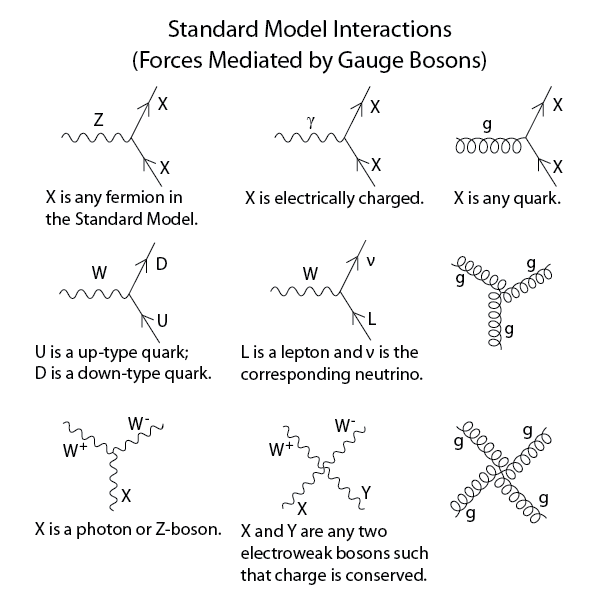
\includegraphics[width=0.75\textwidth]{Standard_Model_Feynman_Diagram_Vertices.png}
	\caption{A list of the vertices that appear in Standard Model Feynman Diagrams. Higgs Boson interactions and neutrino oscillations are omitted. Feynman rule values of the vertices are also omitted. \cite{wikipedia_SM_feynman_vertices}}
        \label{fig:SMvertices}
\end{figure}

In the SM, for processes which have longitudinally polarised W and Z bosons in the final state,
the amplitudes of the diagrams containing the Higgs Boson and of those containing TGC and QGC between electroweak bosons are separately divergent at high energies.
However, their interference between their amplitudes cancels out exactly these divergencies, maintaining the cross section finite on the whole energy spectrum.
This exact cancellation is essential to ensure the ultimate consistency of the theory, as any deviation would eventually lead to violations of the unitarity at high energies \cite{PhysRevLett.38.883}.

In the Standard Model, there are only 4 QGC allowed between electroweak bosons: $\mathrm{WWWW}$, $\mathrm{WWZZ}$, $\mathrm{WWZ\gamma}$ and $\mathrm{WW\gamma\gamma}$ (Figure \ref{fig:EWQGC}).
\begin{figure}[ht]
  \centering
  \subfigure[$\mathrm{WWWW}$]          {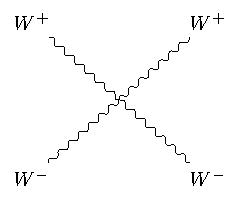
\includegraphics[width=.2\linewidth]{quartic_WWWW.pdf}}
  \subfigure[$\mathrm{WWZZ}$]          {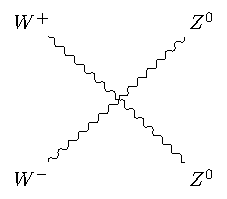
\includegraphics[width=.2\linewidth]{quartic_WWZZ.pdf}}
  \subfigure[$\mathrm{WWZ\gamma}$]     {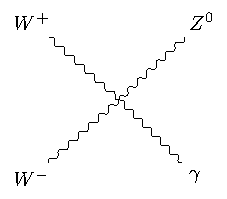
\includegraphics[width=.2\linewidth]{quartic_WWZG.pdf}}
  \subfigure[$\mathrm{WW\gamma\gamma}$]{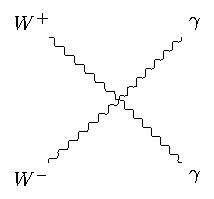
\includegraphics[width=.2\linewidth]{quartic_WWGG.pdf}}
  \caption{Electroweak Quartic Gauge Couplings allowed in the Standard Model.}
  \label{fig:EWQGC}
\end{figure}

There are several processes that are sensitive to TGCs, where their contribution is present at Leading Order (LO) in the perturbative calculations,
but for QGC they are fewer and have very small cross sections.
One of such processes is the Vector Boson Scattering (VBS).
Another process that depends on TGC and QGC at tree level is the simultaneous production of three vector bosons.

\subsection{Triboson production at LHC}
The simultaneous production of three electroweak bosons is a class of extremely rare processes that offer an interesting insight into the mechanisms of the electroweak sector of the Standard Model.
Triboson are extremely rare events which involve the simultaneous emission of three electroweak gauge bosons -- photons, W and Z bosons -- from a single hard scattering event.
The importance of these processes is due to the fact that most of them have a significant contribution from Triple Gauge Couplings (TGC) and Quartic Gauge Couplings (QGC) at Leading Order (LO).
In particular, very few processes are accessible at an hadron collider are sensitive to QGC at tree level.

A few representative Feynman diagrams for triboson production are shown in Figure \ref{fig:triboson_feynman}.
\begin{figure}[th]
  \centering
  \subfigure[]                                 {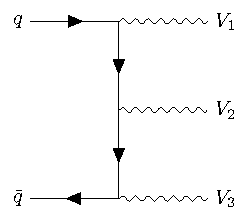
\includegraphics[width=.24\linewidth]{triboson_quarkline_VVV.pdf}}
  \subfigure[]                                 {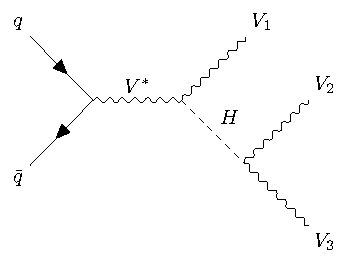
\includegraphics[width=.24\linewidth]{triboson_H_VVV.pdf}}
  \subfigure[\label{fig:triboson_feynman:TGC}] {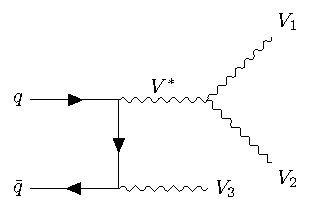
\includegraphics[width=.24\linewidth]{triboson_TGC_VVV.pdf}}
  \subfigure[\label{fig:triboson_feynman:QGC}] {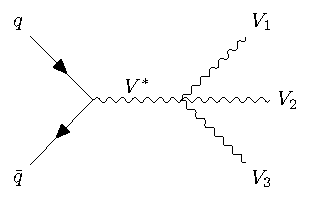
\includegraphics[width=.24\linewidth]{triboson_QGC_VVV.pdf}}
  \caption{Representative Feynman diagrams for the production of three vector bosons. Diagrams \ref{fig:triboson_feynman:TGC} and \ref{fig:triboson_feynman:QGC} are sensitive to triple and quartic gauge couplings respectively.}
  \label{fig:triboson_feynman}
\end{figure}
It must be noted that not all final states are possible through such diagrams, since charge must be conserved at each vertex, the Higgs boson does not directly couple with photons and no fully neutral vertex is allowed in the SM.
This means that no contribution from QGC (Figure \ref{fig:triboson_feynman:QGC}) is present at LO for fully neutral final states such as $\PZ\PZ\PZ$, $\PZ\PZ\PGg$, $\PZ\PGg\PGg$.

It offers the opportunity to test the predictions of the Standard Model with unparalleled precision in a complementary way with respect to the study of the Higgs Boson.

Due to the strikingly low cross section the study of these processes is extremely challenging,
although some have final states with a very low background.

\begin{table}[ht]
  \centering
  \caption{Summary of the ATLAS and CMS collaborations results on triboson production.}
  \label{tab:summary_triboson_papers}
  \renewcommand{\arraystretch}{1.5} % more space between rows in the main table
  \begin{tabular}{l l r l}
    % the nested tables use the normal spacing
    \toprule
    Experiment & Channel(s) & Energy & Significance \\
    \midrule
    ATLAS \cite{STDM-2013-05} & $W\gamma\gamma$                &  8 TeV & $> 3 \sigma$                              \\ \hline
    ATLAS \cite{STDM-2014-01} & $Z\gamma, Z\gamma\gamma$       &  8 TeV & $Z\gamma\gamma$: 6.3 $\sigma$             \\ \hline
    ATLAS \cite{STDM-2015-07} & $WWW$                          &  8 TeV & 0.96 $\sigma$                             \\ \hline
    ATLAS \cite{STDM-2016-05} & $WW\gamma, WZ\gamma$           &  8 TeV & $WW\gamma$ \small{(lept.)}: 1.4 $\sigma$  \\ \hline
    ATLAS \cite{STDM-2016-06} & $\gamma\gamma\gamma$           &  8 TeV & MC overestimate                           \\ \hline
    CMS   \cite{SMP-15-008}   & $W\gamma\gamma, Z\gamma\gamma$ &  8 TeV & \renewcommand{\arraystretch}{1.}\begin{tabular}{@{}l@{}}
      $W\gamma\gamma$: 2.6 $\sigma$\\ $Z\gamma\gamma$: 5.9 $\sigma$
    \end{tabular} \\ \hline
    ATLAS \cite{STDM-2017-22} & $WWW, WWZ, WZZ$                & 13 TeV & \renewcommand{\arraystretch}{1.}\begin{tabular}{@{}l@{}}
      \textbf{combined}: 4.1 $\sigma$\\ WWW \small{(lept.+semilept.)}: 3.2 $\sigma$\\ WVZ \small{(lept.+semilept.)}: 3.2 $\sigma$
    \end{tabular} \\ \hline
    ATLAS \cite{HDBS-2019-16} & $WWW$                          & 13 TeV & 8 $\sigma$, excess over SM at 2.6 $\sigma$\\ \hline
    ATLAS \cite{STDM-2021-09} & $Z\gamma\gamma$                & 13 TeV &                                           \\ \hline
    CMS   \cite{SMP-17-013}   & $WWW$                          & 13 TeV & 0.6 $\sigma$                              \\ \hline
    CMS   \cite{SMP-19-014}   & $WWW, WWZ, WZZ, ZZZ$           & 13 TeV & \renewcommand{\arraystretch}{1.}\begin{tabular}{@{}l@{}}
      \textbf{combined}: 5.0 $\sigma$\\ WWW: 2.5 $\sigma$\\ WWZ: 3.5 $\sigma$\\ WZZ: 1.6 $\sigma$\\ ZZZ: 0 $\sigma$
    \end{tabular} \\ \hline
    CMS   \cite{SMP-19-013}   & $W\gamma\gamma, Z\gamma\gamma$ & 13 TeV & \renewcommand{\arraystretch}{1.}\begin{tabular}{@{}l@{}}
      $W\gamma\gamma$: 3.1 $\sigma$\\ $Z\gamma\gamma$: 4.8 $\sigma$
    \end{tabular} \\
    \bottomrule
  \end{tabular}
\end{table}
% CMS
% SMP-15-008 & WGG, ZGG           &  8 TeV & WWG: 2.6, ZGG: 5.9                                  & http://dx.doi.org/10.1007/JHEP10(2017)072
%
% SMP-17-013 & WWW                & 13 TeV & 0.6 sigma                                           & http://dx.doi.org/10.1103/PhysRevD.100.012004
% SMP-19-014 & WWW, WWZ, WZZ, ZZZ & 13 TeV & combined: 5.0, WWW: 2.5, WWZ: 3.5, WZZ: 1.6, ZZZ: 0 & http://dx.doi.org/10.1103/PhysRevLett.125.151802
% SMP-19-013 & WGG, ZGG           & 13 TeV & WGG: 3.1, ZGG: 4.8                                  & http://dx.doi.org/10.1007/JHEP10(2021)174
%
% SMP-22-006 & WWG, HG            & 13 TeV & 5.6 sigma                                           & submitted https://cds.cern.ch/record/2875047
%
%
% ATLAS
% STDM-2013-05 & WGG           &  8 TeV & evidence, cross section & https://journals.aps.org/prl/abstract/10.1103/PhysRevLett.115.031802
% STDM-2014-01 & ZG, ZZG       &  8 TeV & 6.3 sigma               & https://journals.aps.org/prd/abstract/10.1103/PhysRevD.93.112002
% STDM-2015-07 & WWW           &  8 TeV & 0.96 sigma              & https://link.springer.com/article/10.1140/epjc/s10052-017-4692-1
% STDM-2016-05 & WWG, WZG      &  8 TeV & WWG(lept): 1.4 sigma    & https://link.springer.com/article/10.1140/epjc/s10052-017-5180-3
% STDM-2016-06 & GGG           &  8 TeV & MC overestimate         & https://www.sciencedirect.com/science/article/pii/S0370269318302533
%
% STDM-2017-22 & WWW, WWZ, WZZ & 13 TeV & & https://www.sciencedirect.com/science/article/pii/S0370269319306355
% HDBS-2019-16 & WWW           & 13 TeV & 8 sigma, excess at 2.6 sigma & https://journals.aps.org/prl/abstract/10.1103/PhysRevLett.129.061803
% STDM-2021-09 & ZGG           & 13 TeV & & https://link.springer.com/article/10.1140/epjc/s10052-023-11579-8
%
% STDM-2018-33 & WGG           & 13 TeV & & submitted https://atlas.web.cern.ch/Atlas/GROUPS/PHYSICS/PAPERS/STDM-2018-33
% STDM-2019-17 & WZG           & 13 TeV & & submitted https://atlas.web.cern.ch/Atlas/GROUPS/PHYSICS/PAPERS/STDM-2019-17

Some triboson production channels have been observed by both the ATLAS and CMS collaborations in proton-proton collisions at LHC.
The first results were obtained during \Run1 at a centre-of-mass energy of 8\TeV.

% Many articles only report a fiducial cross section, so it is more difficult to compare between experiments
% GGG
The production of three photons, $\gamma\gamma\gamma$, was observed by the ATLAS Collaboration \cite{STDM-2016-06}, with a measured cross section of $72.6 \pm 6.5 \text{(stat)} \pm 9.2 \text{(syst)}~\text{fb}$.
% WGG
Evidence for the production of $W\gamma\gamma$ was found by the ATLAS Collaboration \cite{STDM-2013-05} measuring a cross-section of $6.1^{+1.1}_{-1.0} \text{(stat)} \pm 1.2 \text{(syst)} \pm 0.2 \text{(lumi)}~\text{fb}$ for the leptonic channel,
while the CMS Collaboration \cite{SMP-15-008} measured $4.9 \pm 1.4 \text{(stat)} \pm 1.6 \text{(syst)} \pm 0.1 \text{(lumi)}~\text{fb}$.
% ZGG
Both the ATLAS \cite{STDM-2014-01} and CMS collaborations \cite{SMP-15-008} observed $Z\gamma\gamma$, measuring fiducial cross sections of
$6.2^{+1.2}_{-1.1} \text{(stat)} \pm 0.4 \text{(syst)} \pm 0.1 \text{(lumi)}~\text{fb}$ for the former,
and $12.4 \pm 1.4 \text{(stat)} \pm 1.8 \text{(syst)} \pm 0.3 \text{(lumi)}~\text{fb}$ for the latter for the leptonic decay of the Z boson.
% WWG
The ATLAS Collaboration studied the $WW\gamma$ \cite{STDM-2016-05}, measuring the inclusive cross section $\sigma(pp \rightarrow e\nu \mu\nu \gamma) = 1.5 \pm 0.9 \text{(stat)} \pm 0.5 \text{(syst)}~\text{fb}$, at 1.4 $\sigma$ level.
% WWW
Similarly, the ATLAS Collaboration set an upper limit of 730 fb \cite{STDM-2015-07} on the cross section of $W^{\pm}W^{\pm}W^{\mp}$ at 95 \% confidence level.
% by considering two decay channels, the fully leptonic $W^{\pm}W^{\pm}W^{\mp} \rightarrow \ell^{\pm} \nu \ell^{\pm} \nu \ell^{\mp} \nu$
% and the the semileptonic $W^{\pm}W^{\pm}W^{\mp} \rightarrow \ell^{\pm} \nu \ell^{\pm} \nu j j$.

In \RunII, with more data avaliable, and also the higher centre-of-mass energy of 13\TeV, more channels became accessible.
% WGG
The CMS Collaboration found evidence for $W^\pm\gamma\gamma$ \cite{SMP-19-013} and measured a fiducial cross section of
$13.6^{+1.9}_{-1.9} \text{(stat)} {}^{+4.0}_{-4.0} \text{(syst)} \pm 0.08 \text{(PDF + scale)}~\text{fb}$.
% ZGG
The ATLAS Collaboration observed $Z\gamma\gamma$ \cite{STDM-2021-09} and measured the fiducial cross section $\sigma_{Z(\rightarrow \ell\ell)\gamma\gamma} = 2.45 \pm 0.20 \text{(stat)} \pm 0.22 \text{(syst)} \pm 0.04 \text{(lumi)}~\text{fb}$,
while the CMS Collaboration found evidence for the same process \cite{SMP-19-013} and measured $5.41^{+0.58}_{-0.55} \text{(stat)} {}^{+0.64}_{-0.70} \text{(syst)} \pm 0.06 \text{(PDF + scale)}~\text{fb}$.
% VVV
The ATLAS Collaboration found evidence \cite{STDM-2017-22} and the CMS Collaboration observed \cite{SMP-19-014} the production of three massive vector bosons by combining multiple channels.
The former analysis considered $WWW$ and $WWZ$, measuring the inclusive cross sections
$\sigma_{WWW} = 0.65^{+0.16}_{-0.15} \text{(stat)} {}^{+0.16}_{-0.14} \text{(syst)}~\text{fb}$ and
$\sigma_{WWZ} = 0.55 \pm 0.14 \text{(stat)} {}^{+0.15}_{-0.13} \text{(syst)}~\text{fb}$ respectively,
finding evidence also for the two process separately.
The latter combined $WWW$, $WWZ$, $WZZ$ and $ZZZ$, measuring and inclusive cross section of $1010^{+210}_{-200}\text{(stat)}{}^{+150}_{-120}\text{(syst)}~\text{fb}$.
The individual $WWW$ and $WWZ$ channels also passed the threshold for evidence, and their cross section were measured as
$\sigma_{WWW} = 590 ^{+160}_{-150} \text{(stat)} {}^{+16}_{-130} \text{(syst)}~\text{fb}$ and
$\sigma_{WWZ} = 300 ^{+120}_{-100} \text{(stat)} {}^{+50}_{-40 } \text{(syst)}~\text{fb}$
respectively, while for $WZZ$ the significance was lower than 3 standard deviations with a measured
$\sigma_{WZZ} = 200 ^{+160}_{-110} \text{(stat)} {}^{+70}_{-20 } \text{(syst)}~\text{fb}$,
and for $ZZZ$ only an upper limit of $\sigma_{ZZZ} < 200~\text{fb}$ at 95 \% CL could be placed.
% WWW
In another paper, the ATLAS Collaboration presented the observation of $WWW$ production \cite{HDBS-2019-16},
measuring an inclusive cross-section of $820 \pm 100 \text{(stat)} \pm 80 \text{(syst)}~\text{fb}$,
with an excess approximately 2.6 standard deviations from the predicted cross section of $511 \pm 18~\text{fb}$ calculated at next-to-leading-order QCD and leading-order electroweak accuracy.

The strategy for the measurement of three yet unexplored channels of triboson production will be described in this thesis.

\section{Choice of the final state}
In this thesis a study of triboson production with two massive bosons and a photon is presented.

Vector bosons are unstable particles and, according to the Standard Model, can decay into a pair of leptons or quarks,
which build up the final state observed in the detectors.
In Table \ref{tab:VB-BR} the branching ratios (BR) of W and Z are reported.

\begin{table}
  \centering
  \caption{Branching ratios of vector bosons \cite{Workman:2022ynf}. Note: $\ell$ = e, $\mu$.}
  \label{tab:VB-BR}
  \begin{tabular}{ l r } % l -> divide intermediate and final state
    \hline
    Process & Branching ratio \\
    \hline
    $W \rightarrow e^+ \nu               $ &         (10.71 $\pm$ 0.16) \% \\
    $W \rightarrow \mu^+ \nu             $ &         (10.63 $\pm$ 0.15) \% \\
    $W \rightarrow \tau^+ \nu            $ &         (11.38 $\pm$ 0.21) \% \\
    \boldmath$W \rightarrow \ell \nu     $ & \textbf{(21.34 $\pm$ 0.22) \%}\\
    \boldmath$W \rightarrow q\bar{q}     $ & \textbf{(67.41 $\pm$ 0.27) \%}\\
    \hline
    $Z \rightarrow e^+ e^-               $ &         (3.363 $\pm$ 0.004) \% \\
    $Z \rightarrow \mu^+ \mu^-           $ &         (3.366 $\pm$ 0.007) \% \\
    $Z \rightarrow \tau^+ \tau^-         $ &         (3.370 $\pm$ 0.008) \% \\
    $Z \rightarrow \nu^+ \nu^-           $ &         (20.00 $\pm$ 0.050) \% \\
    \boldmath$Z \rightarrow \ell^+ \ell^-$ & \textbf{(6.729 $\pm$ 0.008) \%}\\
    \boldmath$Z \rightarrow q\bar{q}     $ & \textbf{(69.91 $\pm$ 0.060) \%}\\
    \hline
  \end{tabular}
\end{table}

Hadronic branching ratios are much greater than the leptonic ones: the hadronic BR for the W boson is three times the one containing at least an electron or a muon, while for Z it is 10 times larger.
Triboson production in the $\PZ\PZ\PGg$ and $\PZ\PW\PGg$ channels is an extremely rare process, as highlighted by the cross sections reported in Table \ref{tab:xsection-inclusive}.
On one hand we would like to use the decays with larger BR, but on the other hand with a clean fully leptonic final state it would be easier to separate the signal from the background.
However, the small BR (V $\rightarrow$ leptons) translates into very low production and decay cross section of $\PZ\PZ\PGg$ and $\PW\PZ\PGg$ into leptons (Table \ref{tab:xsection-exclusive}).
In addition the leptonic decay of a W boson produces a charged lepton and a neutrino, but the latter cannot be detected directly neither in CMS nor in ATLAS.
Its presence may only be deduced from the existence of an unbalance in the sum in the transverse plane of the momenta of all the particles coming from a collision,
called ``missing transverse momentum'' (\ptmiss), ``missing transverse energy'', or sometimes just ``missing energy'' (\ETmiss), abbreviated as MET.
Since the measurement of the \ptmiss is by its nature indirect, the errors associated with it are higher than for every other reconstructed entity.
As a result, searches for leptonic decays of \PW bosons suffer from the increased complexity of its reconstruction, especially in the case of two {\PW}s.
Additionally, \ptmiss is present in many different processes besides triboson production, which results in increased background.

In this analysis three channels are considered, with 4, 3, and 2 charged leptons (electrons or muons) in the final state, corresponding to
$pp \rightarrow \PZ\PZ\PGg \rightarrow 4\Pl \PGg$,
$pp \rightarrow \PW\PZ\PGg \rightarrow 3\Pl \PGn \PGg$ and
$pp \rightarrow V\PZ\PGg \rightarrow 2\Pl \PGg\ 2j$ (where $V$ is either \PZ or \PW)
respectively.

\begin{table}
  \centering
  \caption{Cross sections of triboson production and prediction of the number of events in a scenario where the integrated luminosity is 137 fb$^{-1}$.}
  \label{tab:xsection-inclusive}
  \begin{tabular}{ l c c }
    \toprule
    Process & Cross section  & \renewcommand{\arraystretch}{1.}\begin{tabular}{@{}c@{}} Events \\ $\Lumi = 137 fb^{-1}$\end{tabular} \\
    \midrule
    $\Pp\Pp \to \PZ\PZ\PGg$ & $22.02$\usep fb & $3\,016$ \\
    $\Pp\Pp \to \PW\PZ\PGg$ & $34.06$\usep fb & $4\,666$ \\
    \bottomrule
  \end{tabular}
\end{table}

\begin{table}
  \centering
  \caption{Exclusive cross sections of triboson production in the leptonic and semileptonic final states.
    Taus are excluded, meaning that $\Pl = \Pe, \PGm$.
  }
  \label{tab:xsection-exclusive}
  \begin{tabular}{ l@{}l l r } % l -> divide intermediate and final state
    \toprule
    \multicolumn{2}{c}{Process} & Branching ratio & Cross section \\ %total x BR\\
    \midrule
    $\Pp\Pp \to \PZ\PZ\PGg$ & $\to 4\Pl \PGg$      & 0.444\usep\% & 0.098\usep fb\\ % $0.\overline{4}$\usep\% & 0.09786\usep fb
    $\Pp\Pp \to \PW\PZ\PGg$ & $\to 3\Pl \PGn \PGg$ & 1.435\usep\% & 0.489\usep fb\\
    $\Pp\Pp \to \PZ\PZ\PGg$ & $\to 2\Pl \PGg\ 2j$  & 9.408\usep\% & 2.072\usep fb\\
    $\Pp\Pp \to \PW\PZ\PGg$ & $\to 2\Pl \PGg\ 2j$  & 4.536\usep\% & 1.545\usep fb\\
    \bottomrule
  \end{tabular}
\end{table}

The quarks coming from the decay of the bosons hadronize in timescales comparable to 10$^\text{-15}$ s, producing a spray of particles known as a jet.
The reconstruction and identification of such objects is explained in detail in Section \ref{sec:jets}.
The main drawback of the hadronic channels is that, in a hadron collider, jets are produced with a much higher frequency than leptons,
both as initial/final state radiation, higher order QCD corrections, and by \pileup{} events,
which translates into a much higher number of background events.
The precise reconstruction of jet properties is also more difficult, and it is not possible to distinguish the flavour of the light quark that originated a jet,
and thus separating a Z from a W becomes a very challenging task, compared to leptonic decays.

Figure \ref{fig:triboson_feynman_finalstate} shows three illustrative Feynman diagrams for each of the three channels.
It is worth noting that in the Standard Model the $\PW\PZ\PGg$ (regardless of the decay of the \PW and \PZ) production
has a leading order (perturbative expansion up to $\alpha_{EW}^6$) contribution from triple and quartic gauge couplings,
while that is not the case for $\PZ\PZ\PGg$, due to the absence of neutral TGC and QGC.

\begin{figure}[th]
  \centering
  \subfigure[] {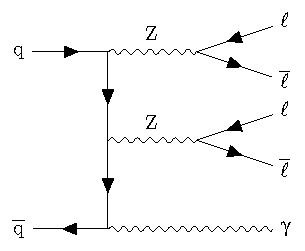
\includegraphics[width=.32\linewidth]{triboson_4LG.pdf}}
  \subfigure[] {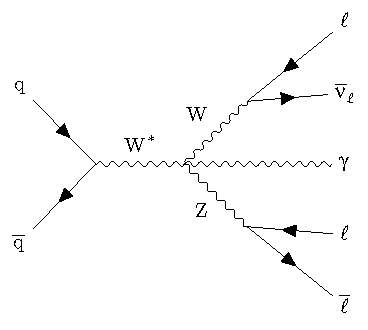
\includegraphics[width=.32\linewidth]{triboson_3LNuG.pdf}}
  \subfigure[] {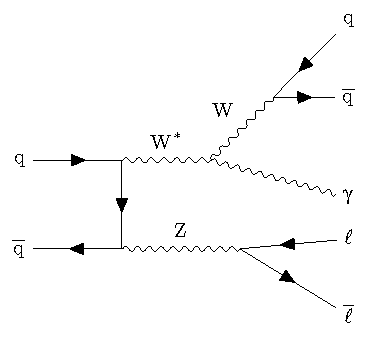
\includegraphics[width=.32\linewidth]{triboson_2L2jG.pdf}}
  \caption{Representative Feynman diagrams for the production of three vector bosons with a photon and 4, 3 or 2 charged leptons in the final state.}
  \label{fig:triboson_feynman_finalstate}
\end{figure}

\clearemptydoublepage
%% CHAPTERS
\chapter{Theoretical framework}
\label{sec:theory}
\section{The Standard Model of particle physics}
The Standard Model (SM) of particle physics is a renormalizable quantum field theory based on gauge invariance principles~\cite{Peskin:1995ev,novaes2000standard}.
The underlying principle is the quantization of the elementary constituents of matter and force carriers,
as excitations of the corresponding quantum fields.
At its core, the Standard Model postulates a set of elementary particles, divided into fermions, with half-integer spin and bosons, with integer spin.
It describes three of the four known fundamental interactions: electromagnetism, the weak nuclear force, and the strong nuclear force.

The fundamental interactions obey a local gauge symmetry, which is associated with a Lie group $U(1)_Y \otimes SU(2)_T \otimes SU(3)_C$,
where Y, T and C denote the quantum numbers hypercharge, weak isospin and colour.

The interactions are mediated by gauge bosons such as the photon, the W and Z bosons and the gluons.
The strong interaction is governed by quantum chromodynamics (QCD), a gauge field theory based on colour symmetry group $SU(3)_C$,
and its eight generators correspond to the gluons.
The electroweak interaction is described by a gauge field theory that is invariant under both weak isospin $T_3$ and hypercharge $Y$,
corresponding to the group $U(1)_Y$ $\otimes SU(2)_T$;
the electroweak interaction encompasses both electromagnetic and weak nuclear interactions,
mediated by the photon and by the \PWp, \PWm and \PZz boson respectively,
which come from the mixing of the generators of the two groups
occurring due to the electroweak symmetry breaking,
as explained later in Section~\ref{EWSB}.
The fundamental bosons all have spin 1, except for the Higgs Boson, which is the only known fundamental particle in the theory with spin 0.

Matter is described in the SM by twelve fermion fields.
All of the fundamental fermions have spin $\frac{1}{2}$ and include quarks, which constitute protons and neutrons, as well as leptons like electrons and neutrinos.
Quarks and leptons are further divided into three generations, each with two particles with different weak isospin, for a total of twelve elementary particles, as detailed in Table \ref{tab:fermions}; each fermion has a corresponding antiparticle with the same mass and spin and opposite charges for the three gauge groups.
Fermions belonging to different generations have been observed to have different masses, which are not predicted by the model and must be determined experimentally.

Quarks have colour charge, anti-quarks carry anti-colour, while leptons have no net colour charge, which is called ``white'' colour.
%% Free particles must have a net colour charge of zero due to colour confinement, which is a property of the strong interaction.
Gluons carry both a colour and an anti-colour charge, while all the other fundamental bosons, as well as bound states of quarks and anti-quarks are white.

Colour charge can exist in three states, arbitrarily labelled blue, green, and red, complemented by an anti-colour, anti-blue, anti-green, and anti-red.

Only the W$^+$ and the W$^-$ bosons carry electromagnetic charge, while the others are neutral.
Only left-handed fermions and right handed anti-fermions can be engaged in charged weak interactions, while the neutral weak interaction can involve both types, although with different couplings.

The Standard Model has not only successfully described a wide range of experimental observations but has also guided the discovery of new particles, like the Higgs boson, which was observed at the Large Hadron Collider in 2012 \cite{ATLASHiggsDiscovery, CMS-HIG-12-028}.
This framework plays a pivotal role in our understanding of the universe, spanning from the conditions just moments after the Big Bang to the inner workings of atomic nuclei.

\begin{table}[tbh]
	\centering
	\caption{Fundamental fermions, classified by family.}
	\label{tab:fermions}
	\begin{tabular}{ c c c c }
		\toprule
		 & 1$^{\text{st}}$ gen. & 2$^{\text{nd}}$ gen. & 3$^{\text{rd}}$ gen. \\%& Electric charge\\
		\midrule
		\multirow{2}{*}{Quarks}  & u       & c         & t          \\%& +$\dfrac{2}{3}$ \\
		                         & d       & s         & b          \\%& -$\dfrac{1}{3}$ \\
		\hline
		\multirow{2}{*}{Leptons} & $\nu_e$ & $\nu_\mu$ & $\nu_\tau$ \\%& 0              \\
		                         & e$^-$   & $\mu$$^-$ & $\tau$$^-$ \\%& -1             \\
		\bottomrule
	\end{tabular}
\end{table}

\begin{table}[th]
  \centering
  \caption{Hypercharge (Y), weak isospin (T$_3$) and electric charge (Q) of fermions. In the table below U and D mean any of the up-type (u,c,t) and down-type (d,s,b) quark, respectively.}
  \label{tab:charges}
  \begin{tabular}{ c c c c }
    \toprule
    & T$_3$ & Y & Q \\
    \midrule \addlinespace
    ${\dbinom{U}{D}}_L$             & $\dbinom{\frac{1}{2}}{-\frac{1}{2}}$ & $\dbinom{\frac{1}{3}}{\frac{1}{3}}$ & $\dbinom{\frac{2}{3}}{-\frac{1}{3}}$ \\ \addlinespace
    $u_R\, ,\  d_R$                 & $+\dfrac{4}{3}\, ,\  -\dfrac{2}{3}$  & $0\, ,\ 0$                          & $+\dfrac{2}{3}\, ,\  -\dfrac{1}{3}$  \\ \addlinespace
    \hline \addlinespace
    ${\dbinom{\nu_\ell}{\ell^-}}_L$ & $\dbinom{\frac{1}{2}}{-\frac{1}{2}}$ & $\dbinom{-1}{-1}$                   & $\dbinom{0}{-1}$                     \\ \addlinespace
    $u_R\, ,\  d_R$                 & $+\dfrac{4}{3}\, ,\  -\dfrac{2}{3}$  & $0\, ,\ 0$                          & $+\dfrac{2}{3}\, ,\  -\dfrac{1}{3}$  \\ \addlinespace
    \bottomrule
  \end{tabular}
\end{table}

\section{Electroweak Symmetry Breaking}
\label{EWSB}
Electromagnetic and weak interactions can be described as a unified electroweak interaction at high energies,
mediated by the massless bosons $B$, that generates $\mathrm{U(1)}_Y$, and $W^{1, 2, 3}$, generators of $\mathrm{SU(2)}_T$.
However, while experiments show that weak interactions are mediated by massive bosons, the inclusion of a mass term of the form $-\frac{1}{2} M^2 W^a_\mu W^{a\, \mu}$ violates the U(1) $\otimes$ SU(2) gauge invariance.
Moreover, the addition in the Lagrangian of a mass term to fermions in the form $-m_q \bar\psi \psi$ would violate the SU(2) invariance, since the left and right handed components of the field $\psi$ behave differently under such gauge transformation.

In 1964 Brout and Englert \cite{PhysRevLett.13.321} and Higgs \cite{PhysRevLett.13.508, HIGGS1964132} indepently proposed
that the spontaneous symmetry breaking, a concept originally elaborated in condensed matter physics, could be the solution to this conundrum.
The Brout-Englert-Higgs Mechanism, shortly called Higgs Mechanism, generates mass terms for gauge bosons while preserving gauge invariance
thought the Electroweak Symmetry Breaking (EWSB).

A new scalar complex field $\Phi$, which is an isospin doublet (with hypercharge $Y_\Phi = 1$) and a colour singlet is introduced.
The Lagrangian of the theory, which is invariant under an original hidden symmetry, is:
\begin{equation}
  %% \begin{split}
  \Lagrangian_{Higgs} = ( D^\mu \Phi )^\dagger ( D_\mu \Phi ) - V(\Phi^\dagger \Phi)\ ,\quad \Phi = \begin{pmatrix} \phi^+ \\ \phi^0 \end{pmatrix}
  %% \end{split}
\end{equation}
Here $V(\Phi^\dagger \Phi)$ is the potential of the field, which is chosen as:
\begin{equation}
  V(\Phi^\dagger \Phi) = \mu^2 \Phi^\dagger \Phi + \lambda (\Phi^\dagger \Phi)^2
\end{equation}
with $\mu^2 < 0$ and $\lambda > 0$, which results in a non-zero expectation value in the vacuum state,
while the minimum is at $\abs{\Phi}^2 = -\frac{\mu^2}{2\lambda}$.

The term $D^\mu$ is the covariant derivative of the electroweak Lagrangian:
\begin{equation}
  D^\mu = \partial^\mu + \frac{i g'}{2} B^\mu Y + \frac{i g}{2} T_a W^{a \mu}
\end{equation}
where $g$ and $g'$ are the coupling constants associated with the $\mathrm{U(1)}_Y$ and $\mathrm{SU(2)}_T$ groups respectively.

The EWSB causes also a mixing of the gauge boson fields, resulting in:
\begin{equation}
\begin{split}
  \PWpm &= \dfrac{1}{\sqrt{2}} \left( W^1 \mp W^2 \right)
  \\
  \begin{pmatrix} \PGg \\ \PZz \end{pmatrix} &= \begin{pmatrix} \cos\theta_W & \sin\theta_W \\ -\sin\theta_W & \cos\theta_W \end{pmatrix} \begin{pmatrix} B \\ W^3\end{pmatrix}
\end{split}
\end{equation}
The only field that remains massless is the photon, while the other three become massive by interacting with three of the four components of the Higgs field $\psi$ through the Brout-Englert-Higgs Mechanism.
The mass of the W and Z boson is not predicted by the theory,
though they are related by $m_\PW = m_\PZ \cos\theta_W$,
and are determined experimentally.
The W mass is approximately $80.38 \GeV$ and the Z mass $91.19 \GeV$~\cite{Workman:2022ynf}.

From the broken symmetry a new particle emerges, corresponding to the fourth component of the Higgs field: the Higgs Boson.
The remaining (unbroken) symmetry is $U(1)_Q \otimes SU(2)_L$.

Because of the mixing, the resulting electric charge of the fermions, that is the coupling to the photon field, is a combination of the hypercharge and weak isospin.

\section{Triboson production}
\subsection{Motivations}
While most of the phenomenology predicted by the SM has already been tested and measured with great precision, the EWSB remains partially unexplored and its study, in the near future, will be of major interest for the particle physics experiments.

Due to the non-abelian nature of the SU(2) and SU(3) groups, there are triple and quartic self-interactions between their gauge fields.
Indeed, while expanding the Yang-Mills Lagrangian of the gauge bosons:
\begin{equation}
\Lagrangian_{YM} = -\frac{1}{4} W^a_{\mu\nu} W_a^{\mu\nu}\,,
\end{equation}
where
\begin{equation}
W^a_{\mu\nu} = \partial_\mu W^a_\nu - \partial_\nu W^a_\mu + g \epsilon^a_{b c} W^b_\mu W^c_\nu\,,
\end{equation}
self-interaction terms appear, containing the structure constants of the symmetry group
\begin{equation}
  \begin{split}
    \Lagrangian_{YM}^{(3)} &= -g \epsilon_{a b c} (\partial^\mu W^{a \, \nu}) W^b_\mu W^c_\nu
    \\
    \Lagrangian_{YM}^{(4)} &= -g (\epsilon_{a b c} W^b_\mu W^c_\nu) (\epsilon^a_{d e} W^{d\,\mu} W^{e\,\nu})\,.
  \end{split}
\end{equation}

The measurement of triple and quartic gauge couplings (TGC, QGC) of electroweak vector bosons, shown in Figure \ref{fig:SMvertices} bottom left and centre, provides an insight into the non-abelian gauge structure of the electroweak interaction and into the mechanism of the EWSB.
%
\begin{figure}
	\centering
	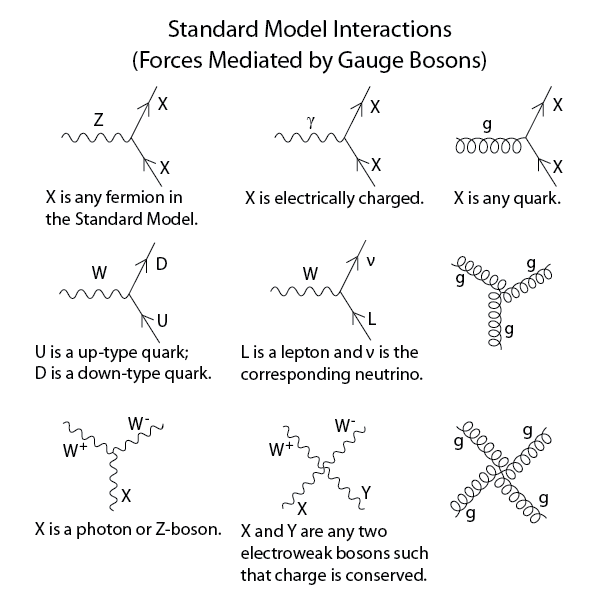
\includegraphics[width=0.75\textwidth]{Standard_Model_Feynman_Diagram_Vertices.png}
	\caption{A list of the vertices that appear in Standard Model Feynman Diagrams. Higgs Boson interactions and neutrino oscillations are omitted. Feynman rule values of the vertices are also omitted. \cite{wikipedia_SM_feynman_vertices}}
        \label{fig:SMvertices}
\end{figure}

In the SM, for processes which have longitudinally polarized W and Z bosons in the final state,
the amplitudes of the diagrams containing the Higgs Boson and of those containing TGC and QGC between electroweak bosons are separately divergent at high energies.
However, their interference between their amplitudes cancels out exactly these divergencies, maintaining the cross section finite on the whole energy spectrum.
This exact cancellation is essential to ensure the ultimate consistency of the theory, as any deviation would eventually lead to violations of the unitarity at high energies \cite{PhysRevLett.38.883}.

In the Standard Model, there are only 4 QGC allowed between electroweak bosons: $\mathrm{WWWW}$, $\mathrm{WWZZ}$, $\mathrm{WWZ\gamma}$ and $\mathrm{WW\gamma\gamma}$ (Figure \ref{fig:EWQGC}).
\begin{figure}[ht]
  \centering
  \subfigure[$\mathrm{WWWW}$]          {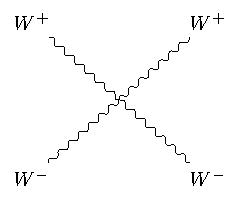
\includegraphics[width=.2\linewidth]{quartic_WWWW.pdf}}
  \subfigure[$\mathrm{WWZZ}$]          {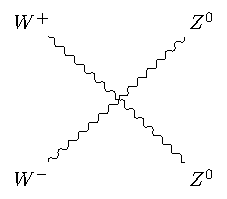
\includegraphics[width=.2\linewidth]{quartic_WWZZ.pdf}}
  \subfigure[$\mathrm{WWZ\gamma}$]     {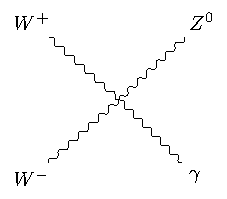
\includegraphics[width=.2\linewidth]{quartic_WWZG.pdf}}
  \subfigure[$\mathrm{WW\gamma\gamma}$]{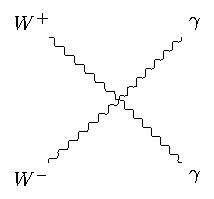
\includegraphics[width=.2\linewidth]{quartic_WWGG.pdf}}
  \caption{Electroweak Quartic Gauge Couplings allowed in the Standard Model.}
  \label{fig:EWQGC}
\end{figure}

There are several processes that are sensitive to TGCs, where their contribution is present at Leading Order (LO) in the perturbative calculations,
but for QGC they are fewer and have very small cross sections.
One of such processes is the Vector Boson Scattering (VBS).
Another process that depends on TGC and QGC at tree level is the simultaneous production of three vector bosons.

\subsection{Triboson production at LHC}
The simultaneous production of three electroweak bosons is a class of extremely rare processes that offer an interesting insight into the mechanisms of the electroweak sector of the Standard Model.
Triboson are extremely rare events which involve the simultaneous emission of three electroweak gauge bosons -- photons, W and Z bosons -- from a single hard scattering event.
The importance of these processes is due to the fact that most of them have a significant contribution from Triple Gauge Couplings (TGC) and Quartic Gauge Couplings (QGC) at Leading Order (LO).
In particular, very few processes are accessible at an hadron collider are sensitive to QGC at tree level.

A few representative Feynman diagrams for triboson production are shown in Figure \ref{fig:triboson_feynman}.
\begin{figure}[th]
  \centering
  \subfigure[]                                 {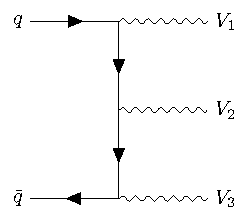
\includegraphics[width=.24\linewidth]{triboson_quarkline_VVV.pdf}}
  \subfigure[]                                 {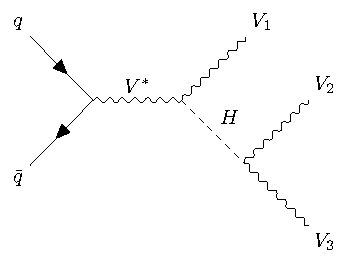
\includegraphics[width=.24\linewidth]{triboson_H_VVV.pdf}}
  \subfigure[\label{fig:triboson_feynman:TGC}] {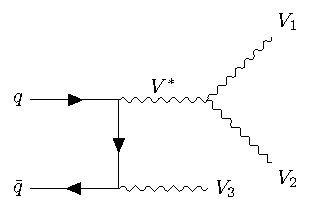
\includegraphics[width=.24\linewidth]{triboson_TGC_VVV.pdf}}
  \subfigure[\label{fig:triboson_feynman:QGC}] {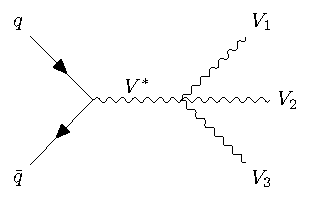
\includegraphics[width=.24\linewidth]{triboson_QGC_VVV.pdf}}
  \caption{Representative Feynman diagrams for the production of three vector bosons. Diagrams \ref{fig:triboson_feynman:TGC} and \ref{fig:triboson_feynman:QGC} are sensitive to triple and quartic gauge couplings respectively.}
  \label{fig:triboson_feynman}
\end{figure}
It must be noted that not all final states are possible through such diagrams, since electric charge must be conserved at each vertex,
the Higgs boson does not directly couple with photons and that the \PZ boson does not interact with the photon, since it is electrically neutral.
This means that no contribution from QGC (Figure \ref{fig:triboson_feynman:QGC}) is present at LO for fully neutral final states such as $\PZ\PZ\PZ$, $\PZ\PZ\PGg$, $\PZ\PGg\PGg$.

It offers the opportunity to test the predictions of the Standard Model with unparalleled precision in a complementary way with respect to the study of the Higgs Boson.

Due to the strikingly low cross section the study of these processes is extremely challenging,
although some have final states with a very low background.

\begin{table}[ht]
  \centering
  \caption{Summary of the ATLAS and CMS collaborations results on triboson production.}
  \label{tab:summary_triboson_papers}
  \renewcommand{\arraystretch}{1.5} % more space between rows in the main table
  \begin{tabular}{l l r l}
    % the nested tables use the normal spacing
    \toprule
    Experiment & Channel(s) & Energy & Significance \\
    \midrule
    ATLAS \cite{STDM-2013-05}  & $\PW\PGg\PGg$                &  8 TeV & $> 3 \sigma$                              \\ \hline
    ATLAS \cite{STDM-2014-01}  & $\PZ\PGg$, $\PZ\PGg\PGg$     &  8 TeV & $\PZ\PGg\PGg$: 6.3 $\sigma$             \\ \hline
    ATLAS \cite{STDM-2015-07}  & $\PW\PW\PW$                  &  8 TeV & 0.96 $\sigma$                             \\ \hline
    ATLAS \cite{STDM-2016-05}  & $\PW\PW\PGg$, $\PW\PZ\PGg$   &  8 TeV & $\PW\PW\PGg$ \small{(lept.)}: 1.4 $\sigma$  \\ \hline
    ATLAS \cite{STDM-2016-06}  & $\PGg\PGg\PGg$               &  8 TeV & MC overestimate                           \\ \hline
    CMS   \cite{CMS-SMP-15-008}&$\PW\PGg\PGg$, $\PZ\PGg\PGg$  &  8 TeV & \renewcommand{\arraystretch}{1.}\makecell[l]{
      $W\PGg\PGg$: 2.6 $\sigma$\\ $Z\PGg\PGg$: 5.9 $\sigma$
    } \\ \hline
    ATLAS \cite{ATLAS-STDM-2018-33}& $\PW\PGg\PGg$            & 13 TeV & 5.6 $\sigma$                              \\ \hline
    ATLAS \cite{ATLAS-STDM-2019-17}& $\PW\PZ\PGg$             & 13 TeV & 6.3 $\sigma$                              \\ \hline
    \noalign{\vspace{.3ex}}
    ATLAS \cite{STDM-2017-22}      & \makecell[l]{$\PW\PW\PW$,\\ $\PW\PW\PZ$, $\PW\PZ\PZ$} & 13 TeV & \renewcommand{\arraystretch}{1.}\makecell[l]{
      \textbf{combined}: 4.1 $\sigma$ \\ $\PW\PW\PW$ \small{(lept.+semilept.)}: 3.2 $\sigma$\\ $\PW{\rm V}\PZ$ \small{(lept.+semilept.)}: 3.2 $\sigma$
    } \\ \noalign{\vspace{.3ex}}\hline
    ATLAS \cite{HDBS-2019-16}      & $\PW\PW\PW$              & 13 TeV & 8 $\sigma$, excess over SM at 2.6 $\sigma$\\ \hline
    ATLAS \cite{STDM-2021-09}      & $\PZ\PGg\PGg$            & 13 TeV &                                           \\ \hline
    CMS   \cite{CMS-SMP-17-013}    & $\PW\PW\PW$              & 13 TeV & 0.6 $\sigma$                              \\ \hline
    \noalign{\vspace{.3ex}}
    CMS   \cite{CMS-SMP-19-014}    & \makecell[l]{$\PW\PW\PW$, $\PW\PW\PZ$,\\ $\PW\PZ\PZ$, $\PZ\PZ\PZ$} & 13 TeV & \makecell[l]{
      \textbf{combined}: 5.0 $\sigma$\\ $\PW\PW\PW$: 2.5 $\sigma$\\ $\PW\PW\PZ$: 3.5 $\sigma$\\ $\PW\PZ\PZ$: 1.6 $\sigma$\\ $\PZ\PZ\PZ$: 0 $\sigma$
    } \\ \noalign{\vspace{.3ex}}\hline
    \noalign{\vspace{.3ex}}
    CMS   \cite{CMS-SMP-19-013}    & $W\PGg\PGg$, $Z\PGg\PGg$ & 13 TeV & \renewcommand{\arraystretch}{1.}\makecell[l]{
      $W\PGg\PGg$: 3.1 $\sigma$\\ $Z\PGg\PGg$: 4.8 $\sigma$
    } \\
    \bottomrule
  \end{tabular}
\end{table}
% CMS
% SMP-15-008 & WGG, ZGG           &  8 TeV & WWG: 2.6, ZGG: 5.9                                  & http://dx.doi.org/10.1007/JHEP10(2017)072
%
% SMP-17-013 & WWW                & 13 TeV & 0.6 sigma                                           & http://dx.doi.org/10.1103/PhysRevD.100.012004
% SMP-19-014 & WWW, WWZ, WZZ, ZZZ & 13 TeV & combined: 5.0, WWW: 2.5, WWZ: 3.5, WZZ: 1.6, ZZZ: 0 & http://dx.doi.org/10.1103/PhysRevLett.125.151802
% SMP-19-013 & WGG, ZGG           & 13 TeV & WGG: 3.1, ZGG: 4.8                                  & http://dx.doi.org/10.1007/JHEP10(2021)174
%
% SMP-22-006 & WWG, HG            & 13 TeV & 5.6 sigma                                           & submitted https://cds.cern.ch/record/2875047
%
%
% ATLAS
% STDM-2013-05 & WGG           &  8 TeV & evidence, cross section & https://journals.aps.org/prl/abstract/10.1103/PhysRevLett.115.031802
% STDM-2014-01 & ZG, ZZG       &  8 TeV & 6.3 sigma               & https://journals.aps.org/prd/abstract/10.1103/PhysRevD.93.112002
% STDM-2015-07 & WWW           &  8 TeV & 0.96 sigma              & https://link.springer.com/article/10.1140/epjc/s10052-017-4692-1
% STDM-2016-05 & WWG, WZG      &  8 TeV & WWG(lept): 1.4 sigma    & https://link.springer.com/article/10.1140/epjc/s10052-017-5180-3
% STDM-2016-06 & GGG           &  8 TeV & MC overestimate         & https://www.sciencedirect.com/science/article/pii/S0370269318302533
%
% STDM-2017-22 & WWW, WWZ, WZZ & 13 TeV & & https://www.sciencedirect.com/science/article/pii/S0370269319306355
% HDBS-2019-16 & WWW           & 13 TeV & 8 sigma, excess at 2.6 sigma & https://journals.aps.org/prl/abstract/10.1103/PhysRevLett.129.061803
% STDM-2021-09 & ZGG           & 13 TeV & & https://link.springer.com/article/10.1140/epjc/s10052-023-11579-8
%
% STDM-2018-33 & WGG           & 13 TeV & & submitted https://atlas.web.cern.ch/Atlas/GROUPS/PHYSICS/PAPERS/STDM-2018-33
% STDM-2019-17 & WZG           & 13 TeV & & submitted https://atlas.web.cern.ch/Atlas/GROUPS/PHYSICS/PAPERS/STDM-2019-17

Some triboson production channels have been observed by both the ATLAS and CMS collaborations in proton-proton collisions at LHC.
The first results were obtained during \Run1 at a centre-of-mass energy of 8\TeV.

% Many articles only report a fiducial cross section, so it is more difficult to compare between experiments
% GGG
The production of three photons, $\gamma\gamma\gamma$, was observed by the ATLAS Collaboration \cite{STDM-2016-06}, with a measured cross section of $72.6 \pm 6.5 \text{(stat)} \pm 9.2 \text{(syst)}~\text{fb}$.
% WGG
Evidence for the production of $W\gamma\gamma$ was found by the ATLAS Collaboration \cite{STDM-2013-05} measuring a cross-section of $6.1^{+1.1}_{-1.0} \text{(stat)} \pm 1.2 \text{(syst)} \pm 0.2 \text{(lumi)}~\text{fb}$ for the leptonic channel,
while the CMS Collaboration \cite{CMS-SMP-15-008} measured $4.9 \pm 1.4 \text{(stat)} \pm 1.6 \text{(syst)} \pm 0.1 \text{(lumi)}~\text{fb}$.
% ZGG
Both the ATLAS \cite{STDM-2014-01} and CMS collaborations \cite{CMS-SMP-15-008} observed $Z\gamma\gamma$, measuring fiducial cross sections of
$6.2^{+1.2}_{-1.1} \text{(stat)} \pm 0.4 \text{(syst)} \pm 0.1 \text{(lumi)}~\text{fb}$ for the former,
and $12.4 \pm 1.4 \text{(stat)} \pm 1.8 \text{(syst)} \pm 0.3 \text{(lumi)}~\text{fb}$ for the latter for the leptonic decay of the Z boson.
% WWG
The ATLAS Collaboration studied the $WW\gamma$ \cite{STDM-2016-05}, measuring the inclusive cross section $\sigma(pp \rightarrow e\nu \mu\nu \gamma) = 1.5 \pm 0.9 \text{(stat)} \pm 0.5 \text{(syst)}~\text{fb}$, at 1.4 $\sigma$ level.
% WWW
Similarly, the ATLAS Collaboration set an upper limit of 730 fb \cite{STDM-2015-07} on the cross section of $W^{\pm}W^{\pm}W^{\mp}$ at 95 \% confidence level.
% by considering two decay channels, the fully leptonic $W^{\pm}W^{\pm}W^{\mp} \rightarrow \ell^{\pm} \nu \ell^{\pm} \nu \ell^{\mp} \nu$
% and the the semileptonic $W^{\pm}W^{\pm}W^{\mp} \rightarrow \ell^{\pm} \nu \ell^{\pm} \nu j j$.

In \RunII, with more data avaliable, and also the higher centre-of-mass energy of 13\TeV, more channels became accessible.
% WGG
The CMS Collaboration found evidence for $W^\pm\gamma\gamma$ \cite{CMS-SMP-19-013} and measured a fiducial cross section of
$13.6^{+1.9}_{-1.9} \text{(stat)} {}^{+4.0}_{-4.0} \text{(syst)} \pm 0.08 \text{(PDF + scale)}~\text{fb}$.
% ZGG
The ATLAS Collaboration observed $Z\gamma\gamma$ \cite{STDM-2021-09} and measured the fiducial cross section $\sigma_{Z(\rightarrow \ell\ell)\gamma\gamma} = 2.45 \pm 0.20 \text{(stat)} \pm 0.22 \text{(syst)} \pm 0.04 \text{(lumi)}~\text{fb}$,
while the CMS Collaboration found evidence for the same process \cite{CMS-SMP-19-013} and measured $5.41^{+0.58}_{-0.55} \text{(stat)} {}^{+0.64}_{-0.70} \text{(syst)} \pm 0.06 \text{(PDF + scale)}~\text{fb}$.
% VVV
The ATLAS Collaboration found evidence \cite{STDM-2017-22} and the CMS Collaboration observed \cite{CMS-SMP-19-014} the production of three massive vector bosons by combining multiple channels.
The former analysis considered $WWW$ and $WWZ$, measuring the inclusive cross sections
$\sigma_{WWW} = 0.65^{+0.16}_{-0.15} \text{(stat)} {}^{+0.16}_{-0.14} \text{(syst)}~\text{fb}$ and
$\sigma_{WWZ} = 0.55 \pm 0.14 \text{(stat)} {}^{+0.15}_{-0.13} \text{(syst)}~\text{fb}$ respectively,
finding evidence also for the two process separately.
The latter combined $WWW$, $WWZ$, $WZZ$ and $ZZZ$, measuring and inclusive cross section of $1010^{+210}_{-200}\text{(stat)}{}^{+150}_{-120}\text{(syst)}~\text{fb}$.
The individual $WWW$ and $WWZ$ channels also passed the threshold for evidence, and their cross section were measured as
$\sigma_{WWW} = 590 ^{+160}_{-150} \text{(stat)} {}^{+16}_{-130} \text{(syst)}~\text{fb}$ and
$\sigma_{WWZ} = 300 ^{+120}_{-100} \text{(stat)} {}^{+50}_{-40 } \text{(syst)}~\text{fb}$
respectively, while for $WZZ$ the significance was lower than 3 standard deviations with a measured
$\sigma_{WZZ} = 200 ^{+160}_{-110} \text{(stat)} {}^{+70}_{-20 } \text{(syst)}~\text{fb}$,
and for $ZZZ$ only an upper limit of $\sigma_{ZZZ} < 200~\text{fb}$ at 95 \% CL could be placed.
% WWW
In another paper, the ATLAS Collaboration presented the observation of $WWW$ production \cite{HDBS-2019-16},
measuring an inclusive cross-section of $820 \pm 100 \text{(stat)} \pm 80 \text{(syst)}~\text{fb}$,
with an excess approximately 2.6 standard deviations from the predicted cross section of $511 \pm 18~\text{fb}$ calculated at next-to-leading-order QCD and leading-order electroweak accuracy.

The strategy for the measurement of three yet unexplored channels of triboson production will be described in this thesis.

\section{Choice of the final state}
In this thesis a study of triboson production with two massive bosons and a photon is presented.

Vector bosons are unstable particles and, according to the Standard Model, can decay into a pair of leptons or quarks,
which build up the final state observed in the detectors.
In Table \ref{tab:VB-BR} the branching ratios (BR) of W and Z are reported.

\begin{table}
  \centering
  \caption{Branching ratios of vector bosons \cite{Workman:2022ynf}. Note: $\ell$ = e, $\mu$.}
  \label{tab:VB-BR}
  \begin{tabular}{ l r } % l -> divide intermediate and final state
    \hline
    Process & Branching ratio \\
    \hline
    $W \rightarrow e^+ \nu               $ &         (10.71 $\pm$ 0.16) \% \\
    $W \rightarrow \mu^+ \nu             $ &         (10.63 $\pm$ 0.15) \% \\
    $W \rightarrow \tau^+ \nu            $ &         (11.38 $\pm$ 0.21) \% \\
    \boldmath$W \rightarrow \ell \nu     $ & \textbf{(21.34 $\pm$ 0.22) \%}\\
    \boldmath$W \rightarrow q\bar{q}     $ & \textbf{(67.41 $\pm$ 0.27) \%}\\
    \hline
    $Z \rightarrow e^+ e^-               $ &         (3.363 $\pm$ 0.004) \% \\
    $Z \rightarrow \mu^+ \mu^-           $ &         (3.366 $\pm$ 0.007) \% \\
    $Z \rightarrow \tau^+ \tau^-         $ &         (3.370 $\pm$ 0.008) \% \\
    $Z \rightarrow \nu^+ \nu^-           $ &         (20.00 $\pm$ 0.050) \% \\
    \boldmath$Z \rightarrow \ell^+ \ell^-$ & \textbf{(6.729 $\pm$ 0.008) \%}\\
    \boldmath$Z \rightarrow q\bar{q}     $ & \textbf{(69.91 $\pm$ 0.060) \%}\\
    \hline
  \end{tabular}
\end{table}

Hadronic branching ratios are much greater than the leptonic ones: the hadronic BR for the W boson is three times the one containing at least an electron or a muon, while for Z it is 10 times larger.
Triboson production in the $\PZ\PZ\PGg$ and $\PZ\PW\PGg$ channels is an extremely rare process, as highlighted by the cross sections reported in Table \ref{tab:xsection-inclusive}.
On one hand we would like to use the decays with larger BR, but on the other hand with a clean fully leptonic final state it would be easier to separate the signal from the background.
However, the small BR (V $\rightarrow$ leptons) translates into very low production and decay cross section of $\PZ\PZ\PGg$ and $\PW\PZ\PGg$ into leptons (Table \ref{tab:xsection-exclusive}).
In addition the leptonic decay of a W boson produces a charged lepton and a neutrino, but the latter cannot be detected directly neither in CMS nor in ATLAS.
Its presence may only be deduced from the existence of an unbalance in the sum in the transverse plane of the momenta of all the particles coming from a collision,
called ``missing transverse momentum'' (\ptmiss), ``missing transverse energy'', or sometimes just ``missing energy'' (\ETmiss), abbreviated as MET.
Since the measurement of the \ptmiss is by its nature indirect, the errors associated with it are higher than for every other reconstructed entity.
As a result, searches for leptonic decays of \PW bosons suffer from the increased complexity of its reconstruction, especially in the case of two {\PW}s.
Additionally, \ptmiss is present in many different processes besides triboson production, which results in increased background.

In this analysis three channels are considered, with 4, 3, and 2 charged leptons (electrons or muons) in the final state, corresponding to
$pp \rightarrow \PZ\PZ\PGg \rightarrow 4\Pl \PGg$,
$pp \rightarrow \PW\PZ\PGg \rightarrow 3\Pl \PGn \PGg$ and
$pp \rightarrow V\PZ\PGg \rightarrow 2\Pl \PGg\ 2j$ (where $V$ is either \PZ or \PW)
respectively.

\begin{table}
  \centering
  \caption{Cross sections of triboson production and prediction of the number of events in a scenario where the integrated luminosity is 137 fb$^{-1}$.}
  \label{tab:xsection-inclusive}
  \begin{tabular}{ l c c }
    \toprule
    Process & Cross section  & \renewcommand{\arraystretch}{1.}\begin{tabular}{@{}c@{}} Events \\ $\Lumi = 137 fb^{-1}$\end{tabular} \\
    \midrule
    $\Pp\Pp \to \PZ\PZ\PGg$ & $22.02$\usep fb & $3\,016$ \\
    $\Pp\Pp \to \PW\PZ\PGg$ & $34.06$\usep fb & $4\,666$ \\
    \bottomrule
  \end{tabular}
\end{table}

\begin{table}
  \centering
  \caption{Exclusive cross sections of triboson production in the leptonic and semileptonic final states.
    Taus are excluded, meaning that $\Pl = \Pe, \PGm$.
  }
  \label{tab:xsection-exclusive}
  \begin{tabular}{ l@{}l c c } % l -> divide intermediate and final state
    \toprule
    \multicolumn{2}{c}{Process} & Branching ratio & Cross section \\ %total x BR\\
    \midrule
    $\Pp\Pp \to \PZ\PZ\PGg$ & $\to 4\Pl \PGg$      & 0.444\usep\% & 0.098\usep fb\\ % $0.\overline{4}$\usep\% & 0.09786\usep fb
    $\Pp\Pp \to \PW\PZ\PGg$ & $\to 3\Pl \PGn \PGg$ & 1.435\usep\% & 0.489\usep fb\\
    $\Pp\Pp \to \PZ\PZ\PGg$ & $\to 2\Pl \PGg\ 2j$  & 9.408\usep\% & 2.072\usep fb\\
    $\Pp\Pp \to \PW\PZ\PGg$ & $\to 2\Pl \PGg\ 2j$  & 4.536\usep\% & 1.545\usep fb\\
    \bottomrule
  \end{tabular}
\end{table}

The quarks coming from the decay of the bosons hadronize in timescales comparable to 10$^\text{-15}$ s, producing a spray of particles known as a jet.
The reconstruction and identification of such objects is explained in detail in Section \ref{sec:jets}.
The main drawback of the hadronic channels is that, in a hadron collider, jets are produced with a much higher frequency than leptons,
both as initial/final state radiation, higher order QCD corrections, and by \pileup{} events,
which translates into a much higher number of background events.
The precise reconstruction of jet properties is also more difficult, and it is not possible to distinguish the flavour of the light quark that originated a jet,
and thus separating a Z from a W becomes a very challenging task, compared to leptonic decays.

Figure \ref{fig:triboson_feynman_finalstate} shows three illustrative Feynman diagrams for each of the three channels.
It is worth noting that in the Standard Model the $\PW\PZ\PGg$ (regardless of the decay of the \PW and \PZ) production
has a leading order (perturbative expansion up to $\alpha_{EW}^6$) contribution from triple and quartic gauge couplings,
while that is not the case for $\PZ\PZ\PGg$, due to the absence of neutral TGC and QGC.

\begin{figure}[th]
  \centering
  \subfigure[] {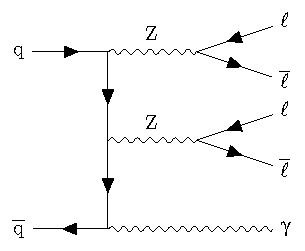
\includegraphics[width=.32\linewidth]{triboson_4LG.pdf}}
  \subfigure[] {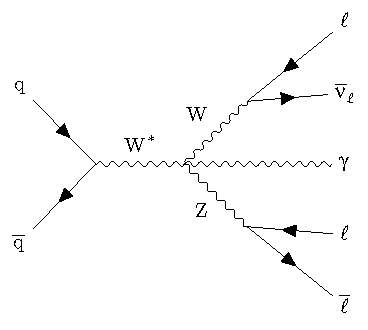
\includegraphics[width=.32\linewidth]{triboson_3LNuG.pdf}}
  \subfigure[] {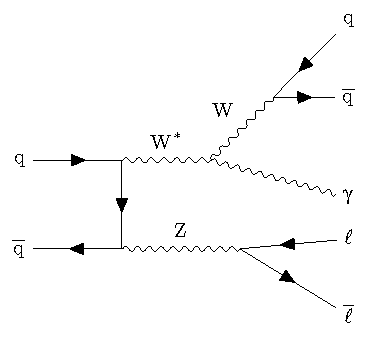
\includegraphics[width=.32\linewidth]{triboson_2L2jG.pdf}}
  \caption{Representative Feynman diagrams for the production of three vector bosons with a photon and 4, 3 or 2 charged leptons in the final state.}
  \label{fig:triboson_feynman_finalstate}
\end{figure}

\clearemptydoublepage
%\chapter[Name in the PDF menu]{Name in the text (and index)}
\chapter{Experimental setup}
\label{sec:experiment}
This thesis uses data obtained through the CMS experiment, which is one of the four major experiments operating at the CERN Large Hadron Collider (LHC).
CERN, the European Organisation for Nuclear Research, was founded in 1954 by a consortium of 12 European countries and its original programme was the study of atomic nuclei.
Over the time, CERN's scientific endeavours have extended in parallel with the understanding of matter, and its current main research area is particle physics: the fundamental constituents and the forces that govern them.
To investigate fundamental interactions, particles are accelerated through a chain of particle accelerators culminating (at the present day) with the LHC.
The collision products are observed and recorded by particle detectors, such as the CMS experiment.

\section{The Large Hadron Collider}
The Large Hadron Collider (LHC) \cite{CERN-AC-93-03-LHC}, situated at the European Organisation for Nuclear Research (CERN) in Geneva, is a two-ring superconducting accelerator designed for high-energy particle collisions.
It operates within a circular underground tunnel 26.7~kilometres long, originally excavated to accommodate the LEP electron-positron collider, operating from 1989 to 2000.

The LHC accelerates two counter-rotating beams, primarily composed of protons but also capable of collision with heavy nuclei like lead (Pb) at varying energies.
The acceleration process involves a sequence of pre-accelerators, shown in Figure \ref{fig:CERNaccelerators}.
The protons are isolated from a duoplasmatron source, accelerated through Linac2 to 50\MeV, further pushed in the Proton Synchrotron Booster (PSB) to 1.4\GeV, accelerated to 25\GeV in the Proton Synchrotron (PS), and finally reach an energy of 450\GeV in the Super Proton Synchrotron (SPS) before entering the LHC rings.

LHC was designed to accelerate protons up to 7\TeV ($\sqrt{s} = 14\TeV$),
and has successfully operated at 3.5 and 4\TeV during \Run1 (2009--2013),
at 6.5\TeV during \Run2 (2015--2018) and 6.8\TeV during the ongoing \Run3 (started in 2022).
Operation at 7\TeV is scheduled for the upcoming High Luminosity LHC (HL-LHC) after the so called ``Long Shutdown 3'', which is foreseen for 2026.

\begin{figure}[htb]
\begin{center}
\includegraphics[width=0.85\textwidth]{Figures/CCC-v2017.png}
\end{center}
\caption{The CERN accelerator complex \cite{OPEN-PHO-ACCEL-2016-009}. The protons start from the LINAC2 and are accelerated by the Booster, the PS and SPS before reaching the LHC.}
\label{fig:CERNaccelerators}
\end{figure}

The LHC's design incorporates various types and sizes of magnets, each serving specific functions: dipole magnets bend the beams,
quadrupole magnets focus the beams in the horizontal and vertical plane,
and sextupole magnets compress the beams closer to the intersection points to increase the likelihood of particle interactions.
This highly sophisticated accelerator operates at temperatures as low as 1.9 K (-271.25 $^\circ$C) by utilizing superfluid helium to cool and maintain the superconducting electromagnets capable of producing magnetic fields of 8.65 T.

Proton bunches in the LHC are spaced by 25 ns and cross at a rate of 40 MHz.
The nominal number of protons per bunch is $N_b = 12 \times 10^{11}$ and the nominal number of bunches is $2808$.
The LHC design luminosity of \LHigh was achieved in 2016, and by the end of 2017 it reached twice this value.
The parameters used by LHC in each year of \RunII{} are reported in Table~\ref{tab:LHCparamsRun2}.

The data recorded by the CMS detector\footnote{
These figures refer to the runs suitable for physics, \eg excluding commisioning, calibrations and special runs, and account for the detector deadtime.
The total luminosity delivered by LHC during the 2016--2018 period is is $159.3\fbinv$.}
corresponds to an integrated luminosity of $36.3\fbinv$ in 2016, $41.5\fbinv$ in 2017 and $59.8\fbinv$ in 2018,
for a total of $137.6\fbinv$.

\begin{table}
  \caption{The main LHC machine parameters for the data production years in \RunII{} compared to the design beam configuration~\cite{CERN-2004-003}.
  The mean number of interactions per bunch crossing (\pileup) denoted with $<\mu>$ is taken from References~\cite{CMS-LUM-17-003, CMS-LUM-17-004, CMS-LUM-18-002}.
  To compare the \pileup{} conditions, the theoretical prediction of the pp inelastic cross-section derived with
  \PYTHIA~\cite{Sjostrand:2015} is used, \ie $\sigma^{13\TeV}_{\text{incl.}}(\Pp\Pp) = 80.0\unit{\text{mb}}$.}
  \label{tab:LHCparamsRun2}
  \centering
  \begin{tabular}{l c c c c}
    \toprule
    Parameter                & Design & 2016 & 2017 & 2018\\
    \midrule
    Beam energy [$\TeV$]     &     7  &  6.5 &  6.5 &  6.5\\
    %% Bunch spacing [ns]      &    25  &  25  & 25   & 25  \\
    $N_p^{bunch}\ [10^{11}]$ &  1.15  & 1.1  & 1.15 & 1.15\\
    $N_{bunches}$            &  2808  & 2220 & 2556 & 2556\\
    $\mathcal{L}_{peak}\ [10^{34}\cm^{-2}\text{s}^{-1}]$ & 1 & 1.4 & 2.06 & 2.01\\
    $<\mu>$                  &    20  &   27 &   38 &   37\\
    \bottomrule
  \end{tabular}
\end{table}

\section{The Compact Muon Solenoid experiment}
The Compact Muon Solenoid (CMS) is one of the two general purpose detectors operating at the LHC.
It is installed in a 100-meter deep cavern situated in the proximity of the French village of Cessy.
The detector was designed to cover a broad scope of physics analyses at the TeV scale, ranging from precision measurements of the electroweak observables to Beyond Standard Model (BSM) searches.
The main feature of the CMS experiment is its superconducting solenoid magnet with 6\usep m internal diameter and 12.5\usep m length, which provides a highly homogeneous magnetic field of 3.8\usep T inside, and around 2\usep T in the steel return yoke.
The high field intensity allows the overall apparatus to be compact, compared to other experiments such as ATLAS, the other LHC general purpose detector.
CMS is 21.6 meters long, 14.6 meter wide and weights 14000 tonnes.

The high bending power is needed to accurately measure the momentum of charged particles up to 1\TeV.
The fine granularity of the CMS detector over a large geometrical coverage allows achieving excellent muon identification and momentum resolution.
The other detector features are the high resolution of the electromagnetic and hadronic calorimeters, and the excellent tracking and vertexing capability.

In order to distinguish between particle signatures, and to provide the most precise measurements of their properties,
CMS was built with concentric layered structure, each subdetector layer targeting a certain interaction type.
A schematic diagram of CMS and its subdetectors is illustrated in Figure \ref{fig:CMSslice}.

\begin{figure}[htb]
\begin{center}
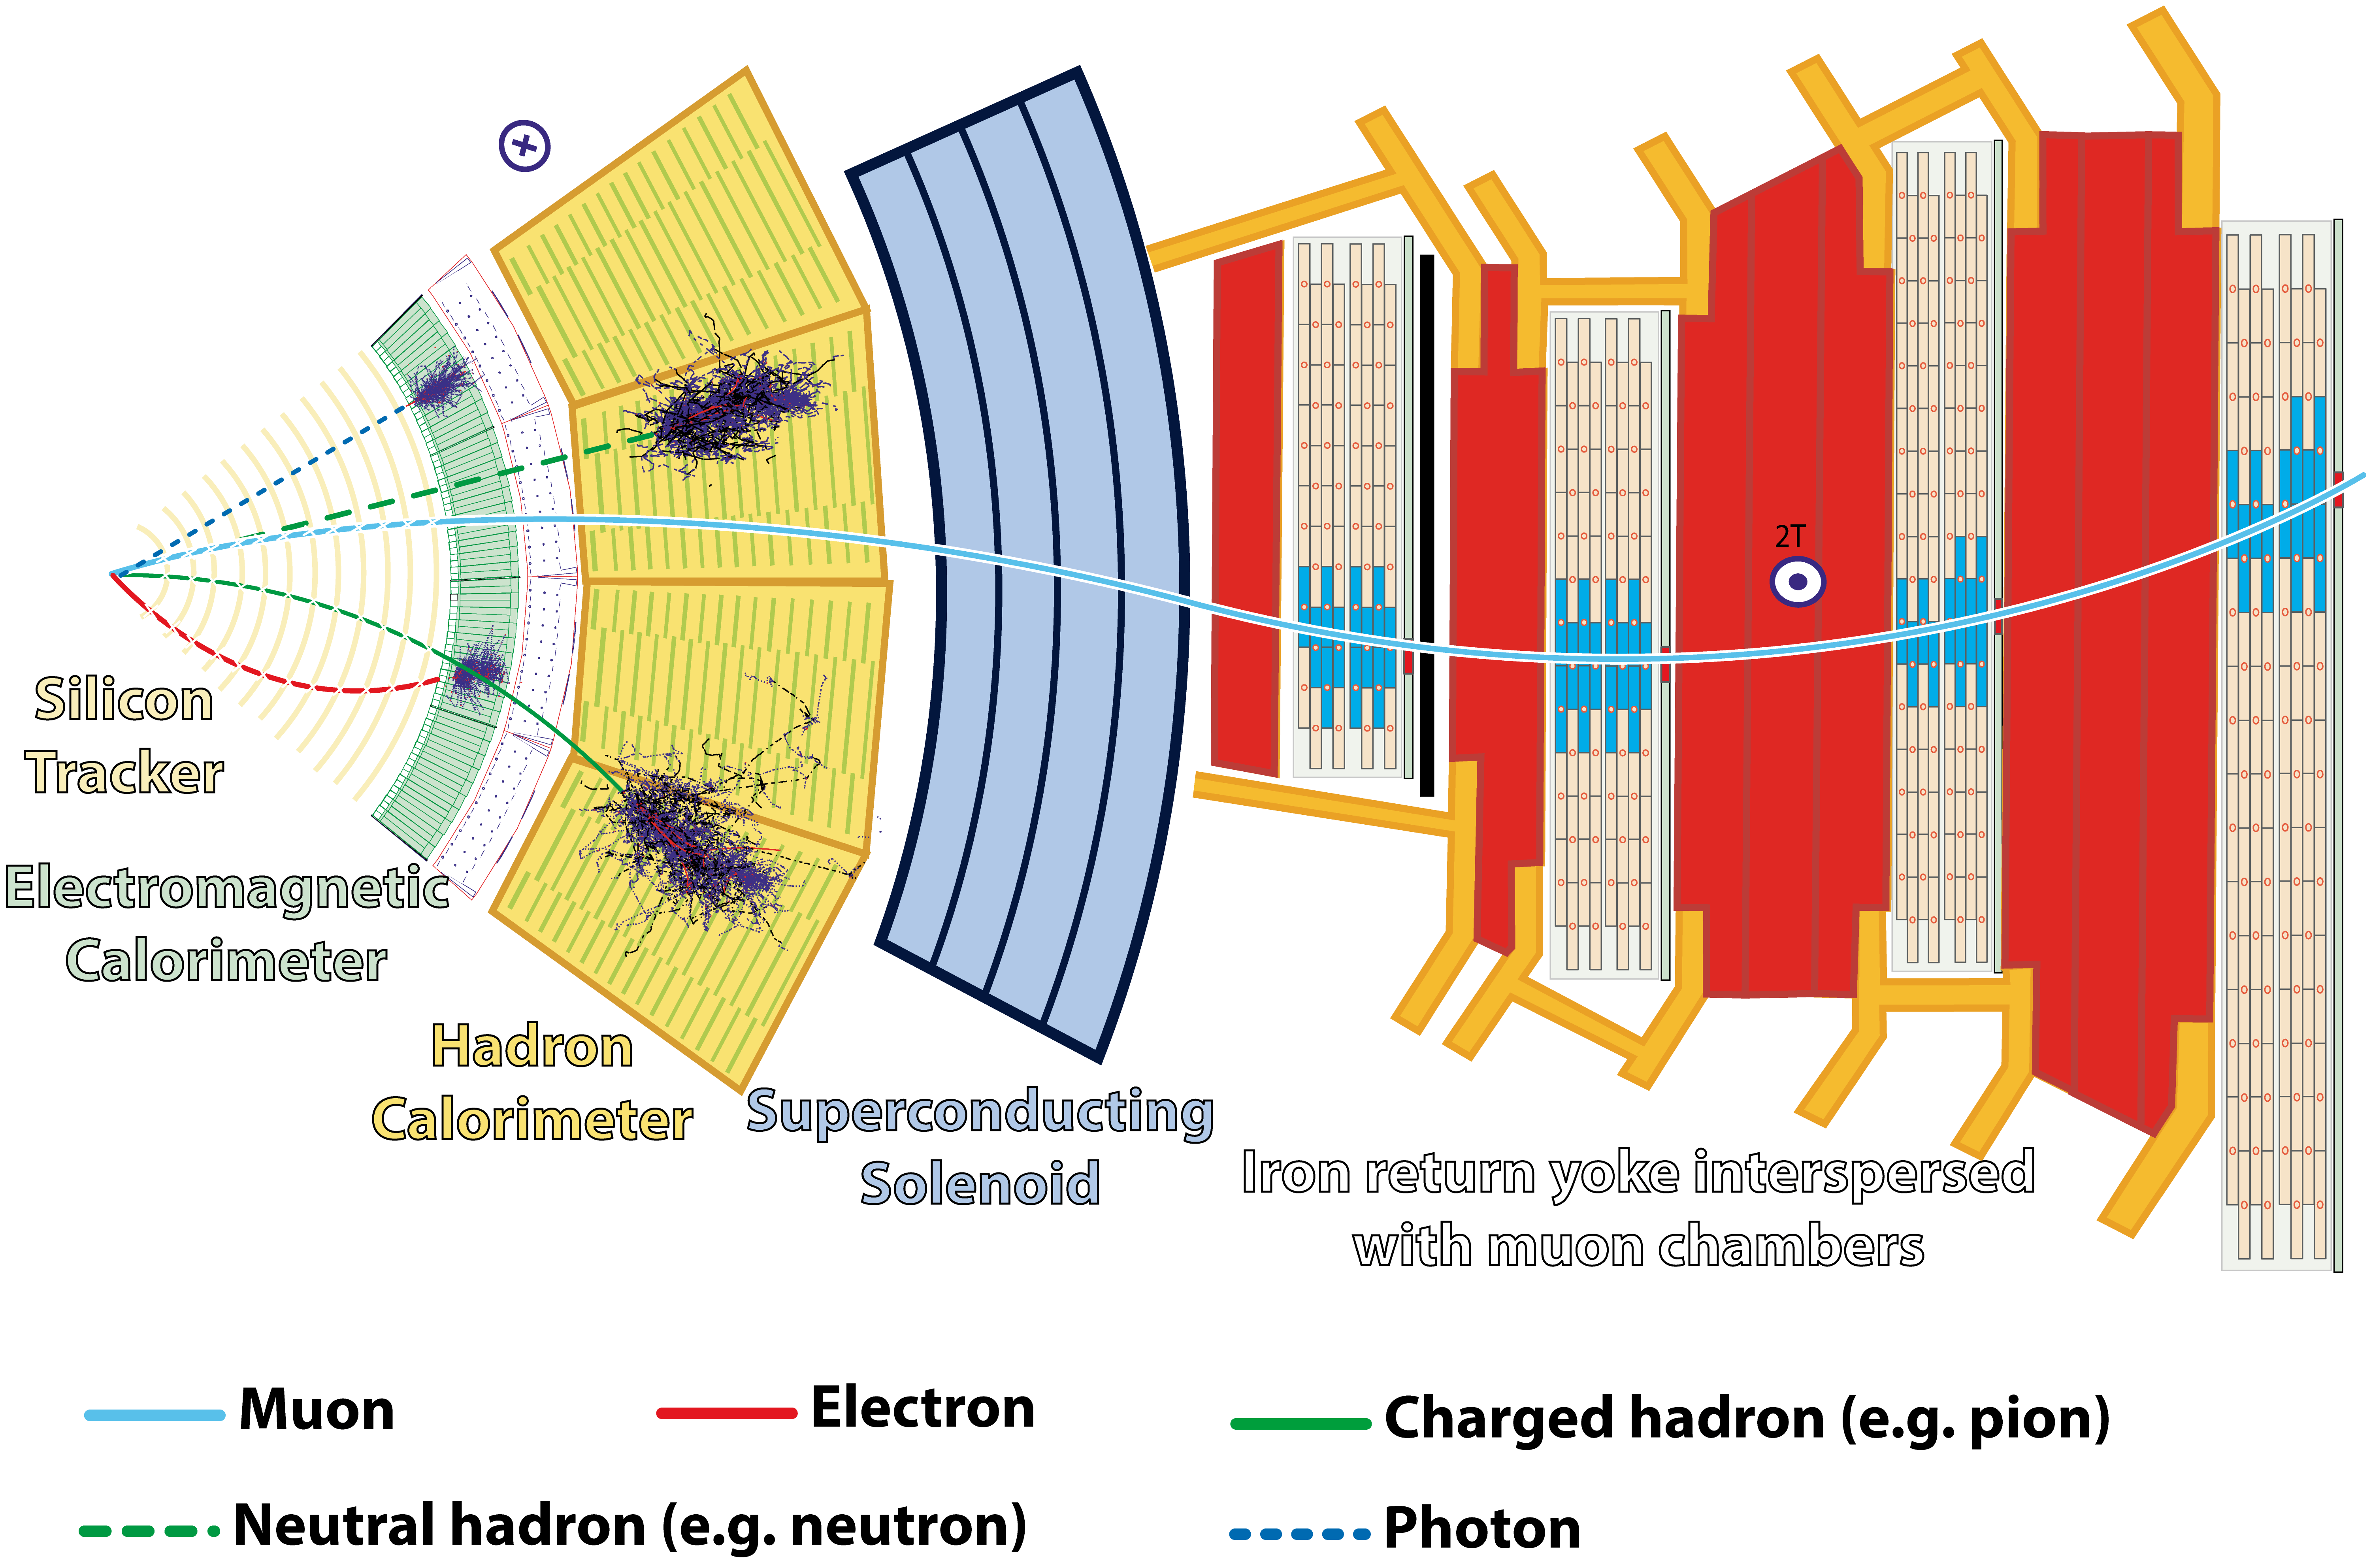
\includegraphics[width=0.85\textwidth]{Figures/CMSslice_whiteBackground.png}
\end{center}
\caption{A simplified transverse view of the CMS detector cross section \cite{CMS-PHO-GEN-2016-001}. The typical signatures of the five particle collections detected are shown.}
\label{fig:CMSslice}
\end{figure}

Within the solenoid volume there are three major subsystems.
A silicon pixel and strip tracker measures the trajectories of charged particles,
a lead tungstate crystal electromagnetic calorimeter (ECAL) mainly collects the energies of electrons and photons,
and a brass and scintillator hadronic calorimeter (HCAL) stops the more penetrating hadrons.
Quartz-fibre-based forward calorimeters further improve hermeticity.
The measurement of the muons properties relies on a combination of inner tracking and the information from the muon chambers,
which are gas-ionization detectors embedded in the steel flux-return yoke outside the solenoid.
A detailed description of the CMS detector can be found in Reference~\cite{CMS-CMS-00-001}.

\paragraph{Coordinate system\\}
CMS adopts a right-handed Cartesian coordinate system, with the origin defined in the centre of the detector; more precisely, the barycentre of the modules of the Tracker Outer Barrel.
The axes are oriented such that the x-axis points to the centre of the LHC ring, the y-axis is orthogonal to the LHC plane pointing up, and the the z-axis lies along the anticlockwise beam direction.

\paragraph{Kinematic variables\\}
In particle physics, the particle polar direction is often described with its rapidity, defined as:
\begin{equation}
  \label{eq:rapidityDefinition}
  y = \frac{1}{2} ln \frac{E + p_z}{E - p_z} \,.
\end{equation}

Difference in rapidity are invariant under Lorentz boosts along the z-axis.
In physics analyses the pseudo-rapidity is often used in its place, since the two coincide in the ultra-relativistic limit:
\begin{equation}
  \label{eq:pseudorapidityDefinition}
  \eta = - ln \left( \tan \frac{\theta}{2} \right) \,,
\end{equation}
where $\theta$ represents the polar angle with respect to the z-axis. The azimuthal angle, measured in the x-y plane is called $\phi$.
They are used to define a type of angular distance between two physical objects:
\begin{equation}
  \label{eq:deltaRDefinition}
  \Delta R = \sqrt{ \Delta \eta^2 + \Delta \phi^2 } \,.
\end{equation}

\subsection{Silicon tracker}
The CMS inner silicon tracker is the innermost subdetector of the CMS experiment, surrounding the interaction point, measuring 5.8 m in length and 2.5 m in diameter.
It provides precise measurement of the trajectories of the charged particles emerging from the LHC collisions.
These tracks are reconstructed by combining electrical signals (hits) from the outgoing charged particles as they traverse the tracker's layers.
Thanks to the uniform magnetic field within its volume, which bends the trajectories, it is able to provide accurate hits measurements,
allowing excellent reconstruction of the associated momentum and charge sign from the track parameters.

The accuracy of track reconstruction is crucial for determining the position of the hard scattering, the primary vertex, as well as in-flight decays resulting in secondary vertices.
This in turns allows for the suppression of the background from \pileup{} interactions,
which are simultaneous collisions between other pairs of protons in the same bunch crossing\footnote{
Strictly speaking, this is called in-time \pileup.
Collisions happening in the previous or next bunch crossing are referred to as out-of-time \pileup.
},
and a handle for measuring particle lifetimes.

The CMS tracker uses silicon pixel and strip sensors to cover $|\eta| < 2.5$, with a total area of $200\, \mathrm{m}^2$,
operating at temperatures of around -15\Celsius and -20\Celsius, respectively, to minimize the impact of the ionizing radiation damage.
To meet spatial measurement requirements amid particle flux, the finely segmented tracking detector with fast readout electronics minimizes the material to reduce multiple scattering.
Silicon's benefits include high charge carrier mobility, rapid signal processing, optimal energy resolution sensitivity, and excellent spatial resolution due to segmentation.
Local hit reconstruction involves clustering, noise calibration, and hit candidate conversion, providing cluster charge profiles and hit positions.

In 2017, the pixel detector underwent an upgrade, enhancing performances with additional layers in both barrel and endcaps \cite{CMS-TDR-11}.
The tracker's overall layout, shown in Figure \ref{fig:PIX_Phase_comparison}, optimally addresses the challenges posed by the LHC collisions.

The CMS tracker is structured in a hierarchical fashion, with a few large mechanical structures composed by smaller parts,
the smallest unit being always the single module.
A full overview of the structure hierarchies of the CMS tracker is shown in Figure \ref{fig:tracker_hierarchy}.

\begin{figure}
  \centering
  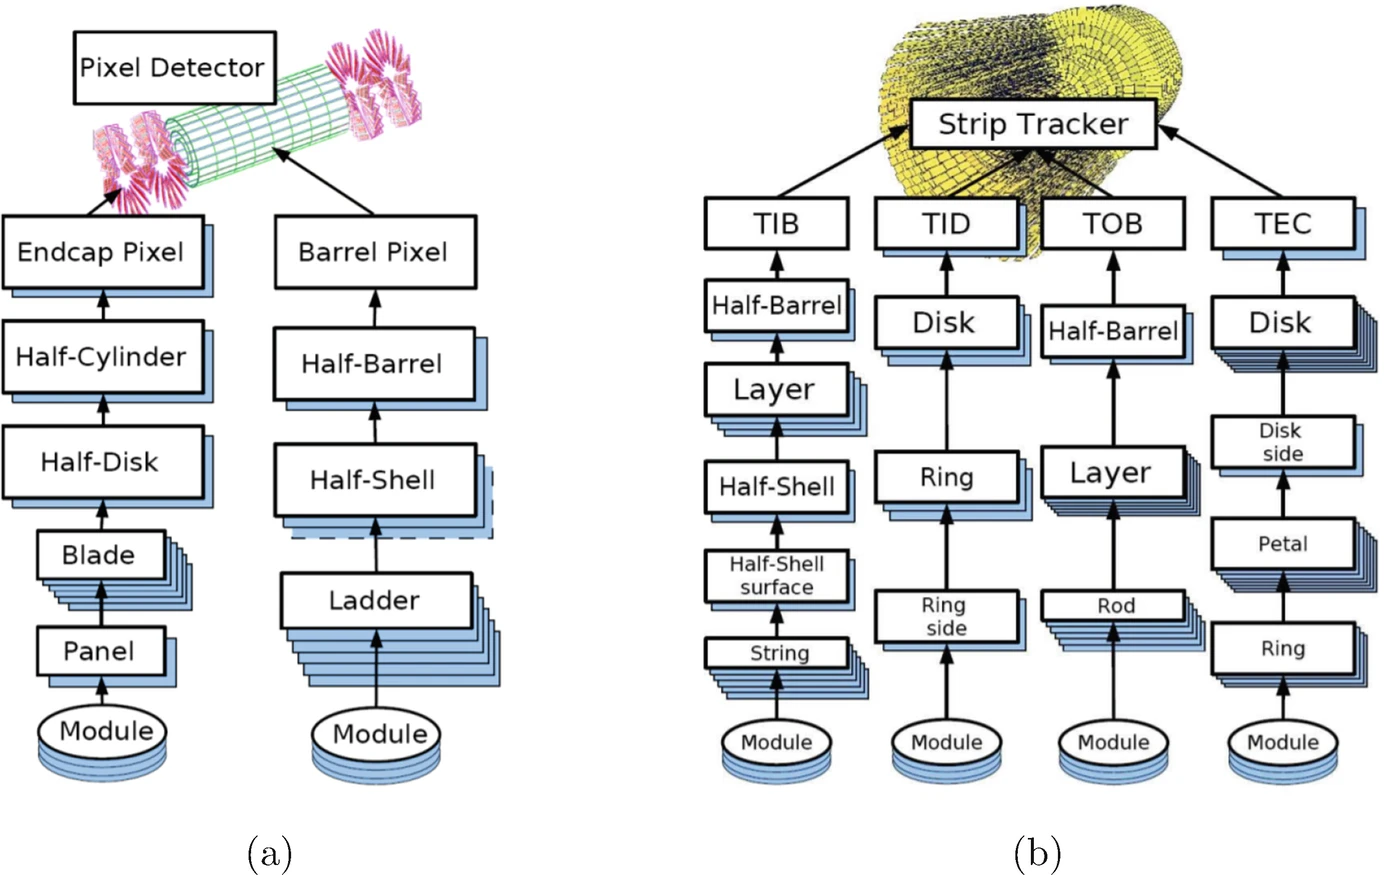
\includegraphics[width=0.85\textwidth]{tracker_hierarchy.png}
  \caption{Hierarchical structure of the CMS tracker, for the pixel (left) and for the strip (right) detectors \cite{CMS-NOTE-2009-002}.}
  \label{fig:tracker_hierarchy}
\end{figure}

\subsubsection{Silicon pixel detector}
The Pixel detector is the innermost tracking subsystem and it consists of two parts, the Barrel Pixel (BPIX) and the Forward Pixel (FPIX) detectors.
The description of the Phase-I pixel follows, and a comparison with the Phase-0 is shown in Figure \ref{fig:PIX_Phase_comparison}.

The BPIX is composed of four coaxial barrel layers located at a radial distance of 2.9, 6.8, 10.9 and 16.0\cm.
The FPIX consists of three endcap disks per side constituted by several blades positioned at a distance of 29.1, 39.6 and 51.6\cm from the nominal interaction point (IP).
The BPIX modules are parallel to the beamline, while the FPIX sensors are arranged into blades, oriented with a tilt of 20$\,^{\circ}$ with respect to normal incidence in order to exploit the Lorentz drift effect\footnote{
Charge carriers in the sensors, migrating along an electric field that is not parallel to the magnetic field, will have their trajectories deflected by a small angle $\theta_{LA}$.
This Lorentz drift effect broadens the charge cluster to neighbouring sensors (charge sharing), thereby improving the hit resolution.
}.

The 124 million pixels, around double the amount of the Phase-0 version, have an individual size of $100 \times 150 \mum^2$.
The front-end modules of the data acquisition (DAQ) system are powered by 1200 DC-DC converters that deliver the necessary voltage in the range of 2.4--3.3\usep V,
which were installed during the upgrade to cope with the increased number of channels while maintaining the existing cabling~\cite{Feld_2015}.
During the last period of data taking of 2017, called era F, 5\usep \% of the converter had failed and 35\usep \% were damaged (but working) due to the radiation damage aggravated by a design problem, and were successfully replaced during the 2017-2018 end-of-year technical stop~\cite{CMS:dcdc-failure-short}.

\begin{figure}[thb]
  \centering
  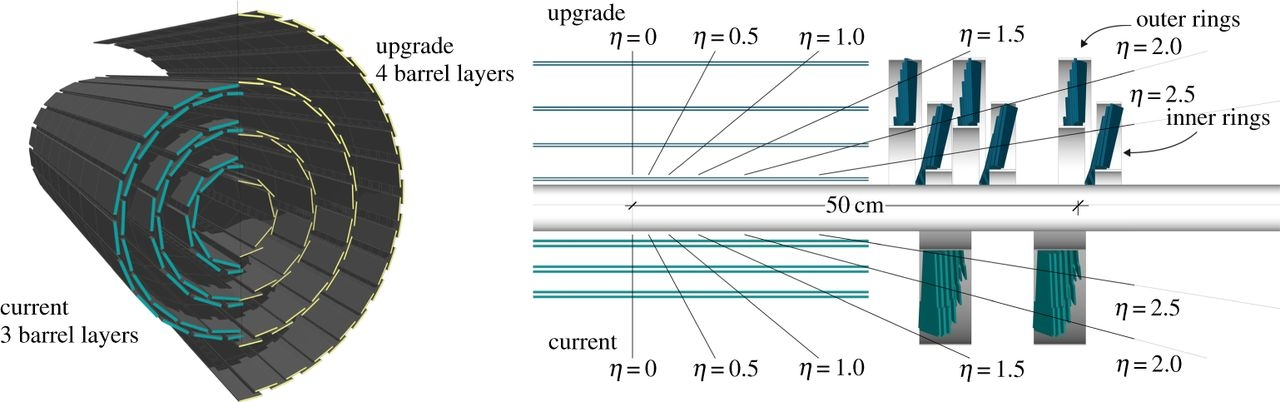
\includegraphics[width=0.85\textwidth]{PIX_Phase_comparison.jpg}
  \caption{A comparison of the different BPIX layers and FPIX disks between the Phase-0 and Phase-1 pixel detectors.}
  \label{fig:PIX_Phase_comparison}
\end{figure}

\subsubsection{Silicon strip detector}
The strip silicon tracker is located outside of the pixel detector at a radial distance comprised between 20 and 116 \cm.
It consists of 15148 silicon modules, with approximately 9.3 million strips and it extends over a pseudorapidity range up to $|\eta| < 2.5$.
The strip subsystem features an analogous barrel-endcap partition as in the case of the pixel detector.
The barrel region is subdivided into the Tracker Inner Barrel (TIB) and the Tracker Outer Barrel (TOB),
while the end-cap system is partitioned into the Tracker Inner Disks (TID) and the Tracker End Cap (TEC).

The inside of the tracker barrel is occupied by the four cylindrical layers of the TIB subdetector,
extending up to $\pm 65 \cm$ along the z axis, and the three TID disks covering up to a radius of $55 \cm$.
The double-sided modules arranged back-to-back present in the first two TIB layers allow for a hit measurement both in cylindrical coordinates
with a $23-34 \mum$ spatial resolution in the $r - \phi$ plane and of $530 \mum$ in the z-direction.
The TIB/TID system is enclosed by the six barrel layers of the TOB, which extends to a radius of $116 \cm$ and up to $\pm 118 \cm$ in the direction of the proton beam.
The TOB sensors are almost a factor two wider than the TIB due to the lower particle fluence.
Coverage in the z region $124 \le |z| \le 282 \cm$ is ensured by the TEC subdetector, composed of nine disks of various sizes,
providing hit positional information in the $r - \phi$ plane with a resolution in the range $18 - 47 \mum$.

\subsection{Electromagnetic calorimeter}
The Electromagnetic Calorimeter (ECAL) \cite{CERN-LHCC-97-033} provides a measurement of the energy of incoming electrons and photons.
It is a hermetic, homogeneous calorimeter made of scintillating crystals of lead tungstate ($\mathrm{PbWO_4}$).
The material was chosen because of its short radiation length (0.89\cm) and high density,
which allow the absorption of electromagnetic showers within the short length;
its small Moli\`ere radius (2.2\cm) allows a good shower separation.
Its response time is fast, and 80 \% of the scintillation light is emitted within the 25 ns between the LHC bunch crossings.
The general structure is shown in Figure \ref{fig:ECAL_3D_colour}.

\begin{figure}[thb]
  \centering
  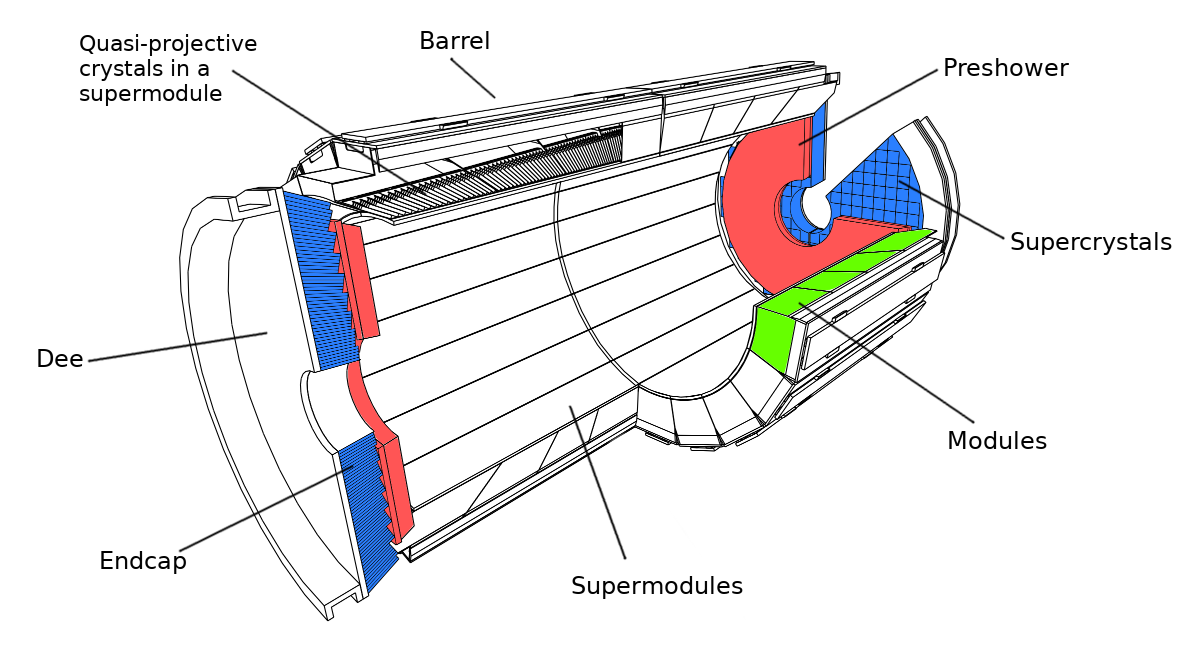
\includegraphics[width=0.85\textwidth]{ECAL_3D_colour.png}
  \caption{A 3D render of ECAL with the main components highlighted \cite{siddireddy2018cms}.}
  \label{fig:ECAL_3D_colour}
\end{figure}

ECAL is composed of Electromagnetic Barrel (EB), Electromagnetic Endacp (EE) and Endcap Preshower (PS).
EB is made of 61200 crystals with a quasi-projective geometry, and each endcap has 7324 crystals.
The EB has an inner radius of $129 \cm$, and it is structured as 36 identical ``Supermodules'',
each covering $20\usep ^{\circ}$ in $\phi$ and half the barrel length, corresponding to a pseudorapidity interval of $0 < |\eta| < 1.479$.
Each supermodule contains four modules with 400 or 500 crystals apiece, each with a length of 230 mm and a cross section of $22 \times 22 \usep \mathrm{mm}^2$.
The EE is at a distance of $314 \cm$ from the vertex and covering a pseudorapidity range of $1.479 < |\eta| < 3.0$,
and is made of crystals with a length of 220 mm and a cross section of $28.62 \times 28.62 \usep \mathrm{mm}^2$.

The crystals have a quasi-projective geometry, with an angle of 3$\usep ^{\circ}$ from the nominal interaction point in both $\theta$ and $\phi$ directions,
to avoid the alignment of inter crystal gaps with particle trajectories.

The scintillation light from ECAL crystals is read by fast, radiation-tolerant photodetectors which can operate inside the CMS magnetic field
and are insensitive to particles traversing them.
Two preshower detectors are installed at each end of the tracker detector, in front of the ECAL endcaps,
in order to help distinguishing $\Pgpz \to \PGg \PGg$ decays from single photons and identifying electrons against minimum ionizing particles.
These sampling calorimeters are made of a lead radiator layer which initiates electromagnetic showers from incoming particles,
followed by silicon strip sensors that measure the deposited energy.
Although lead tungstate crystals are radiation resistant, they undergo a limited but rapid loss of optical transmission under irradiation.
This phenomenon depends on the luminosity and crystal pseudorapidity, and is partly balanced by an annealing effect.
This effect is measured and it is taken into account by time-dependent corrections applied to the measured particle energies.

The ECAL energy resolution $\sigma_E/E$ for electrons was obtained in a test beam measurement \cite{CMS-NOTE-2006-148}, and has the following energy dependency:
\begin{equation}
  \frac{\sigma_E}{E} = \frac{2.8\%}{\sqrt{E\, [\GeV]}} \oplus \frac{12\%}{E\, [\GeV]} \oplus 0.3\% \,,
\end{equation}
where the $\oplus$ symbol denotes the sum in quadrature of the individual contributions.
The first term represents the stochastic part which dominates for energy deposits of photoelectrons below 100\GeV;
the second term stands for the noise contribution;
the constant accounts predominantly for calibration inaccuracies and additionally for the non-uniform response of the photodetectors.

\subsection{Hadronic calorimeter}
The HCAL calorimeter is a sampling detector employed for the measurement of the energy deposits of hadrons.

The central part of the HCAL covers a pseudorapidity range up to $|\eta| < 1.3$ and it consists of two distinct subdetectors:
the inner barrel (HB) part with brass absorbing layers and plastic scintillator tiles,
and the outer hadronic calorimeter (HO) entirely composed of plastic scintillators, installed outside the solenoid.
Because of the limitations in size of the CMS calorimeter, some of the most-energetic hadronic tails may leak outside the full volume of the HB detector.
Thus, the HO subdetector has been installed to extend the depth of the HCAL to 11.8 hadronic interaction lengths
in order to catch the most energetic hadronic shower tails, utilizing the magnet coil as an absorber.

The HCAL endcaps (HE) cover the range $1.3 < |\eta| < 3$ and uses the same brass absorber as HB.
It is required to handle high counting rates and have high radiation tolerance.
Including the EB in front of it, it has a total depth of around 10 interaction lengths.
The scintillation light produced by plastic tiles is collected by wavelength shifting fibres and detected by multipixel hybrid photodiodes.

The hadron forward calorimeter (HF) extends the pseudorapidity range to $|\eta| = 5.2$ and it is located at a distance of 11\usep m from the beamspot.
Since it is affected by hadronic energy depositions seven times more intense than in the rest of the HCAL,
it is composed of iron absorbers and quartz fibre as active material, due to their higher more radiation-hardness.
It is further equipped with a set of photomultipliers, which detect the cone of Cherenkov light emitted by charged particles passing through the material.

The segmentation of the tiles is $\Delta \eta \times \Delta \phi = 0.087 \times 0.087$ for $|\eta| < 1.6$ and $\simeq 0.17 \times 0.17$ for $|\eta| \ge 1.6$.

%% The relative HCAL energy response curve for isolated charged pions is illustrated in Figure 2.8.
%% A broader response curve is an indicator of a larger \pileup{} contamination.
%% Out-of-time \pileup{} mitigation helps reduce the latter, thereby improving the quality of pion isolation.
HCAL is instrumental in recognizing hadrons and their decay products,
and provides a crucial measurement of the missing transverse energy exploiting its extensive coverage in $\eta$, a property referred to as hermeticity.
The HF is also used for two of the methods for measuring the instantaneous luminosity.

\begin{figure}[thb]
  \centering
  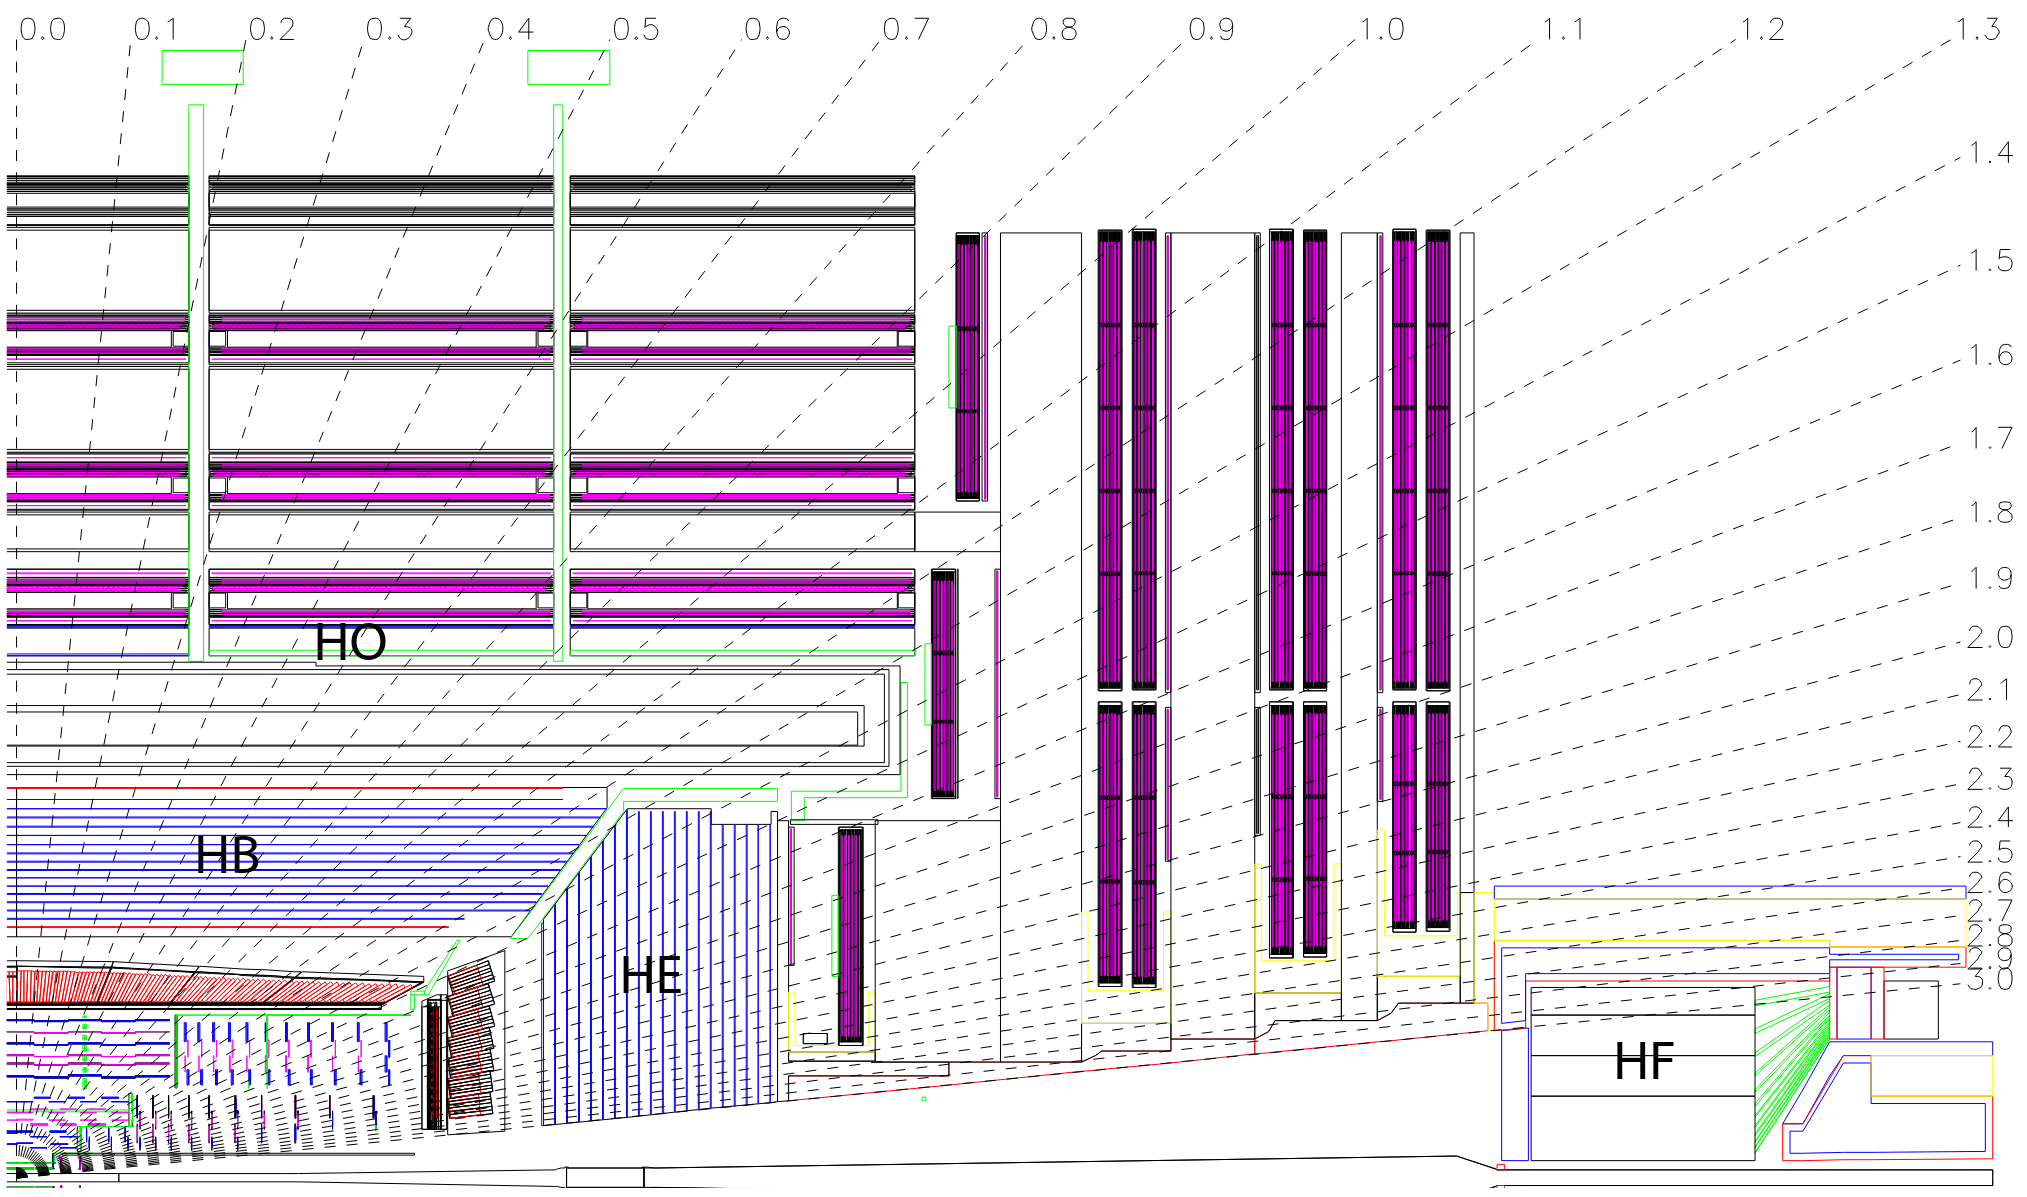
\includegraphics[width=0.85\textwidth]{HCAL_2Dquarter.png}
  \caption{Longitudinal view of the CMS detector showing the locations of the hadron barrel (HB), endcap (HE), outer (HO) and forward (HF) calorimeters. \cite{CMS-CMS-00-001}.}
  \label{fig:HCAL_2Dquarter}
\end{figure}

\subsection{The muon system}
Muons produced in collisions at the LHC usually traverse the Tracker, ECAL, HCAL,
and the solenoid volumes without being stopped and are identified and measured in the muon detectors located in the outermost part of CMS.
The muon system is made of muon chambers embedded in the iron return yoke of the CMS magnetic field
and is divided into a cylindrical barrel section and two planar endcaps.
It uses three types of gas-ionization chambers: Drift Tubes (DT), Cathode Strip Chambers (CSC) and Resistive Plate Chambers (RPC).
A new set of muon detectors using the Gas Electron Multiplier (GEM) technology
and designed to cope with the foreseen increased luminosity of HL-LHC is being installed in the endcap section~\cite{CMS-TDR-013}.
The layout of the three subsystems is shown in Figure \ref{fig:MUON_2Dquarter}.

\begin{figure}[thb]
  \centering
  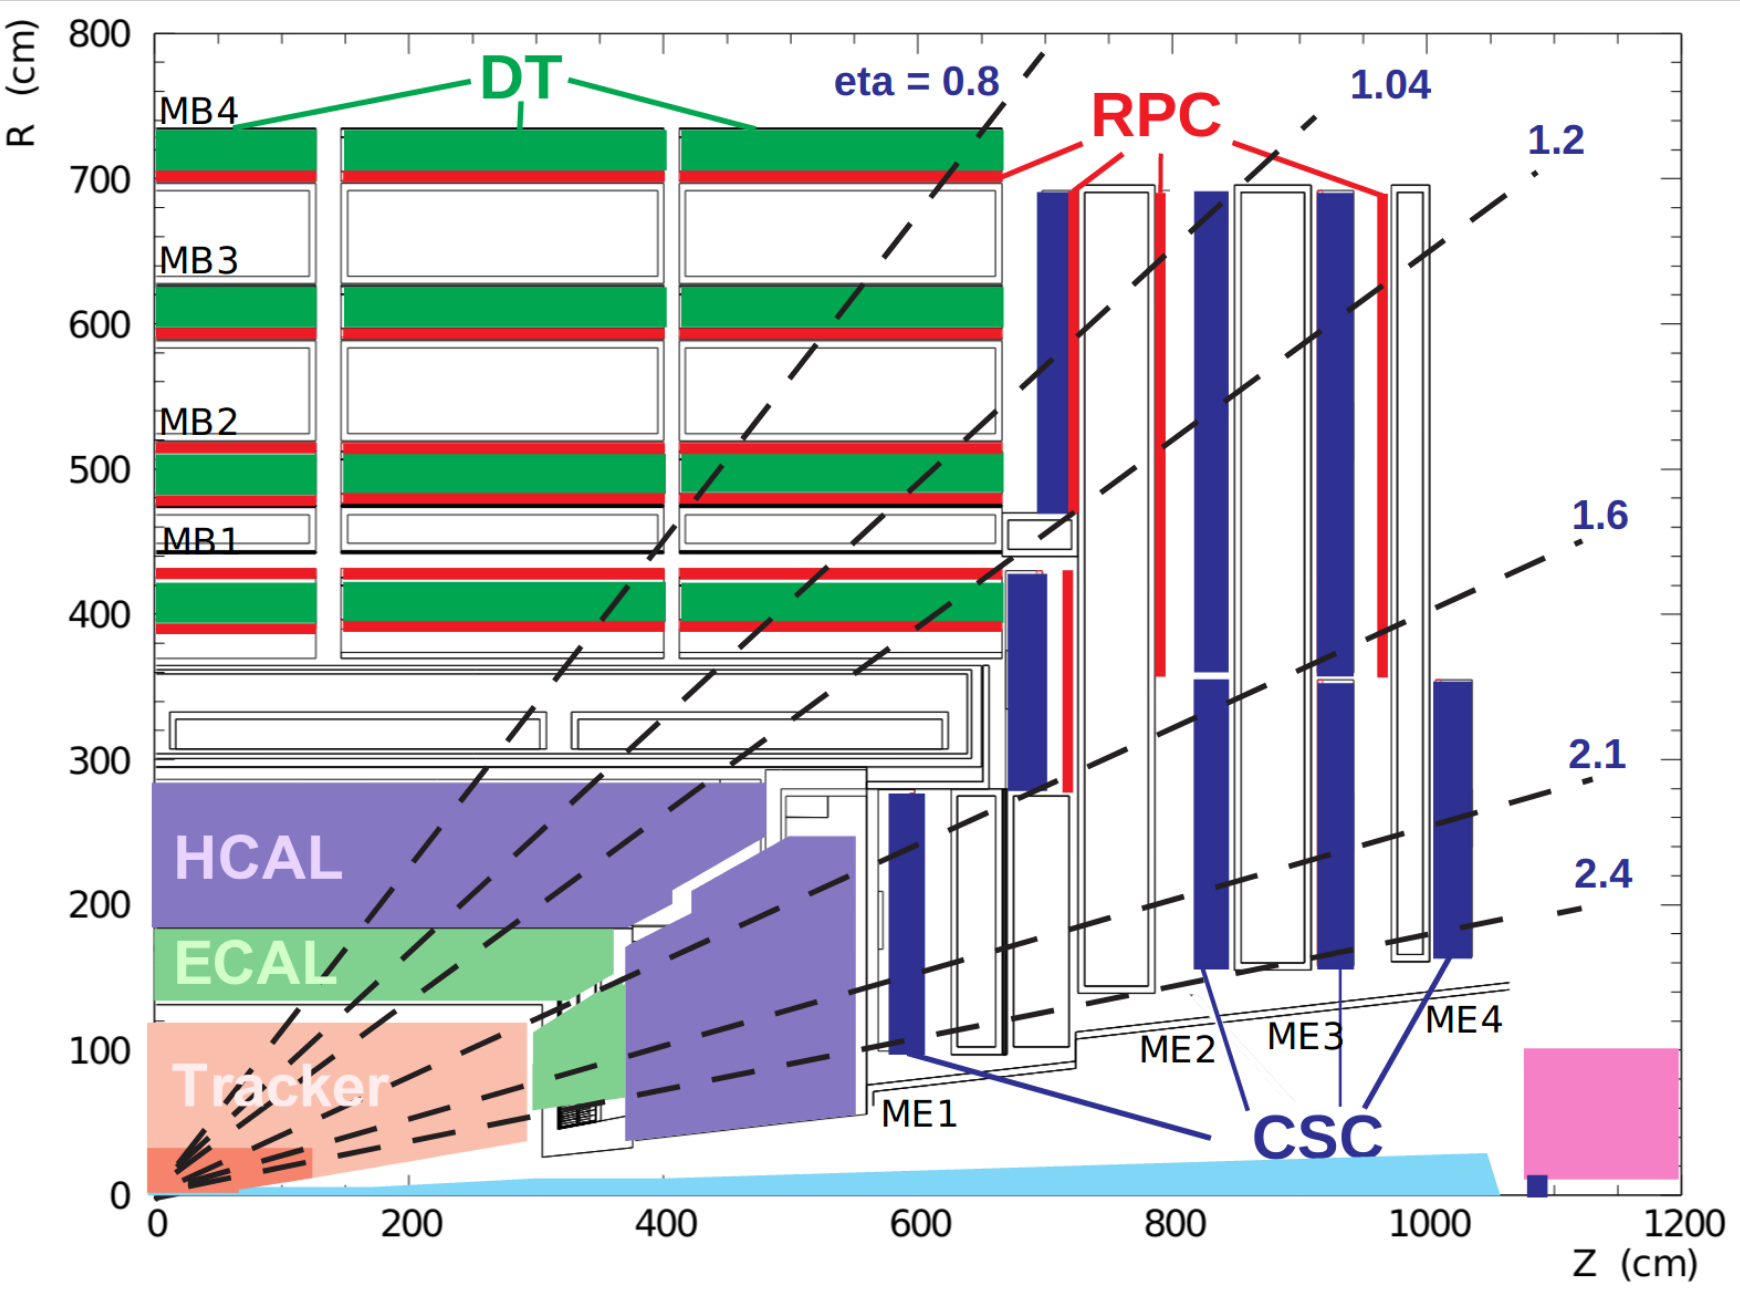
\includegraphics[width=0.85\textwidth]{MUON_2Dquarter.png}
  \caption{Longitudinal layout of one quadrant of the CMS detector.
    The four DT stations in the barrel (MB1–MB4, green),
    the four CSC stations in the endcap (ME1–ME4, blue),
    and the RPC stations (red) are shown~\cite{CMS-MUO-10-004}.}
  \label{fig:MUON_2Dquarter}
\end{figure}

\subsubsection{Drift Tubes}
The Drift Tubes (DTs) are located in the barrel region, where the muon rate is lower and the magnetic field is quite uniform,
and cover a pseudorapidity range of $|\eta| < 1.2$.
The DTs are organized into four stations interspersed among the layers of the flux return plates.
Their basic constituents are rectangular drift cells bounded by two parallel aluminium planes, which serve as cathodes.
Anodes are 80\mum stainless steel wires located in the centre of each cell.
A muon passing through a cell ionizes the gas mixture that fills the cell volume.
The drift time of the resulting electrons is then used to measure the distance between the muon track and the wire.
Each chamber has a resolution of 100 µm in the $r - \phi$ plane.

\subsubsection{Cathode Strip Chambers}
The Cathode Strip Chambers (CSCs) are used in the endcaps, where the the muon rates and background levels are higher and the magnetic field is large and non uniform,
and cover a pseudorapidity range of $0.9 < |\eta| < 2.4$.
The CSCs are multiwire proportional chambers, made of 6 anode wire planes interleaved among 7 cathode panels,
with the wires running approximately perpendicular to the strips.
A muon passing through a chamber generates an avalanche, inducing a charge on several cathode strips.
The ensuing interpolation allows a spatial resolution of 50\mum to be obtained.
Four stations of CSCs are located in each endcap.
The chambers are positioned perpendicular to the beam line and interspersed between the magnetic field flux return plates.

\subsubsection{Resistive Plate Chambers}
The Resistive Plate Chambers (RPCs) are located both in the barrel and in the endcaps and cover the pseudorapidity range $|\eta| < 1.6$.
The RPCs are double-gap chambers which operate in avalanche mode and are disposed in six layers in the barrel and three layers in the endcaps.
They provide a complementary trigger system with moderate spatial resolution but excellent time resolution (of the order of 1 ns),
which helps measuring the correct beam-crossing time.

\subsubsection{Gas Electron Multiplier}
A Gas Electron Multiplier (GEM) consists of a layer of electrically insulated polymer coated with metal and chemically perforated.
A significant voltage is applied between the two metal sides, which results in high electric fields inside the holes,
where electons produced by an ionizing particle in the gas produce an electron avalanche.
A GEM chamber has multiple layers (3 for the ones used in CMS).
A demonstrator, consisting of 144 chabers, has already been installed during Long Shutdown~2 (2019--2021),
after the end of \Run2 and is currently contributing to the \Run3 data taking.

\subsection{Trigger system}
The enormous LHC proton-proton collision rate of 40 MHz with a characteristic event size of approximately 1 MB
is a serious challenge to the CMS Data Acquisition (DAQ) system.
However most of the data refers to low-energy interactions, rather than hard scattering and rare processes.
Thus the need for a system that is able to reduce the huge data flow to a manageable rate prior to storage on disk,
whilst selecting efficiently the interesting events is necessary.
These requirements are met by the so-called CMS triggering system,
which reduces the initial bandwidth by over three orders of magnitude.
The CMS triggering system adopts a sophisticated two-stage approach,
consisting of a \Lone trigger (L1) fully implemented in hardware logic and a high-level trigger (HLT) software farm.
%% The L1 trigger achieves a rate reduction down to the level of 100 kHz, which is subsequently downscaled to around 1 kHz at HLT level.

\subsubsection{Level-1 Trigger}
\label{sec:L1trigger}
The L1 trigger achieves a rate reduction down to the level of 100 kHz, with a latency below 4\mus.
It is implemented in custom hardware, using Field Programmable Gate Arrays (FPGAs) which are generic and easily customizable,
and Application Specific Integrated Circuits (ASICs), which are more resilient to high \pileup{} conditions, albeit not easily reconfigurable.
The \Lone trigger uses information from the calorimeters and the muon system to construct the so called \textit{trigger primitives},
which are the base of the trigger logic.
An overview of the layout of the system is shown in Figure \ref{fig:L1trigger-block-diagram}.

\begin{figure}[thb]
  \centering
  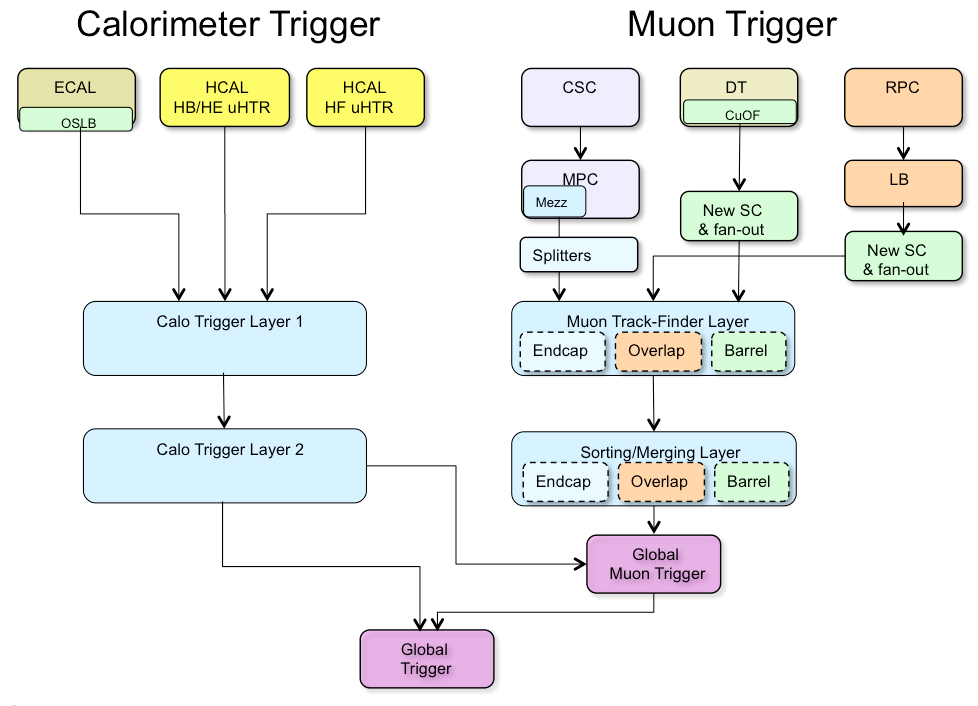
\includegraphics[width=0.85\textwidth]{L1trigger-block-diagram.png}
  \caption{Main data-flow diagram for the Phase-1 \Lone trigger \cite{CMS-TDR-12}.}
  \label{fig:L1trigger-block-diagram}
\end{figure}

\subsubsection{High-level Trigger}
The High Level Trigger (HLT) is a sophisticated software-based system which uses tens of thousands of CPU cores
running multithreaded instances of an optimized version of the CMS reconstruction algorithm~\cite{CMS-TRG-12-001}.
This array of commercial CPUs manages the full event reconstruction through several sequential algorithms,
targeting signature of interest referred to as \textit{trigger path}.
The goal of the HLT is to reduce the incoming \Lone rate of 100 kHZ to around 1 kHz,
while maintaining a good efficiency in the various phase spaces of interest for physics
and being as inclusive as possible to enable a broad variety of searches.

For this purpose, some paths that would otherwise exceed the available bandwidth are made to only pass the selection after a pre-scale.
This consists of a random discarding of the event, either at L1 or at HLT, which is then accounted for in the analysis.

Another major constraint of the HLT is the maximum processing time for each event, which is 50 ms.
To optimize it, the more computationally-intensive algorithms are run at the end of the filtering sequence.
These modules perform a streamlined version of the standard offline reconstruction.

\clearemptydoublepage
\chapter{Reconstruction}

The collision events registered by the CMS detector are reconstructed by combining information from the different subdetectors.
This process aims to improve the identification of the final-state particles and the reconstruction precision of their properties.
The basic elements such as tracks and calorimeter clusters are reconstructed first and form the starting point for the next step.
The global event reconstruction strategy is implemented through the Particle Flow (PF) algorithm \cite{ParticleFlow}.
Originally applied in the ALEPH experiment at LEP, this algorithm combines data from the CMS subsystems to reconstruct physics objects and achieve a comprehensive and coherent event reconstruction.
The resulting particles include charged and neutral hadrons, photons, electrons, muons and taus, serving as the starting inputs for all subsequent data analyses.
Additionally, PF candidates are used to construct more advanced objects such as jets and missing transverse energy.

% NOTE: the content of this chapter is taken (and adapted) from the Analysis Note

%% Electrons and muons are considered candidates for the reconstruction of ZZ final states
%% (``signal leptons'') if  their transverse momentum,
%% $\pt^\ell$, is greater than 7(5)~\GeV and their pseudorapidity,
%% $\left| \eta^\ell \right|$, is less than 2.5 (2.4) for electrons (muons).
%% The physics objects and the ZZ candidate selections used in this analysis are those of the $H \rightarrow ZZ \rightarrow 4\ell$~\cite{HiggsAN,HiggsLegacyPaper} analysis, with minor changes. Here, we just report the main features, referring to that material for control plots/tables etc.

\section{Base elements}
\subsection{Tracks}
\label{sec:tracks}
The reconstruction of the trajectory of charged particles with high precision at the CMS detector
is a complex task because of the large combinatorics from the high multiplicity of particles and the large number of readout channels.

First local charge clusters are converted to hits using the digitised output from the tracker modules.
%% The local track reconstruction output is then buffered for the global track reconstruction, which aims at identifying
%% hit combinations that match to possible trajectories of the charged particles present in the event.
%% Track seeds are built from few hits compatible with a charged particle trajectory (e.g. triplets in the pixel detector).
The tracks reconstruction is based on an iterative pattern recognition technique,
a Kalman-like fitting procedure adapted for the CMS framework in the Combinatorial Track Finder \cite{billoir.qian:simultaneous, Speer:2005dp} (CTF) algorithm.
The Kalman Filter (KF) part of the algorithm carries out three main sub-tasks.
\begin{itemize}
\item \textbf{Seed finding}, involving the generation of the starting points of the iterative sequence, namely pairs or triplets of hits.
\item \textbf{Pattern recognition} iteratively performs the following steps:
  \begin{enumerate}
  \item navigation: the current track parameters are used to determine which adjacent layers of the detector can be intersected by extrapolation;
  \item a search is performed within the layer for modules which are compatible with the trajectory;
  \item groups of hits are formed for each module, and a $\chi^2$ test is used to determine their compatibility with the trajectory;
    for each compatible hit (plus the hypothesis of no hit) a new trajectory candidate is created
  \item the trajectory candidates are updated using the information from the hits collected in the current iteration.
  \end{enumerate}
  A maximum of 5 candidates is retained at each iteration of the pattern recognition.
  %% The procedure is repeated until the outermost tracker layer, or a stopping condition in the HLT version, is reached.
\item \textbf{Final fit}: the best-fit value of the track parameters and the covariance matrix are determined by means of a least-squares fit.
\end{itemize}
The CTF runs several times the KF algorithm.
%% At each iteration of the CTF, positional information from the hits used in the previous step is discarded and the set of requirements are gradually relaxed.
The first types of seeds to be processed are those that are more likely to belong to high-momentum particles with an origin close to the beam axis.
Later iterations target tracks that are missing one or more hits, have low-momentum or originate from a displaced vertex.

At each iteration of the CTF, track candidates must satisfy a series of quality criteria
based on cuts on the track impact parameter significance with respect to the beamspot,
the number of hits in the inner tracking system and the normalised $\chi^2$ of the track trajectory.

After the final fit, the hits of the newly built tracks are masked for the next iterations.
This reduces the combinatorial complexity of the seed finding and the pattern recognition steps,
maintaining a low misreconstruction rate while increasing tracking efficiency, especially at low momentum,
with the the added benefit of reducing the computing time up to a factor 2 (for \RunII{} conditions).


\subsection{Calorimeter clusters}
\label{sec:clusters}
First, \textit{cluster seeds} are identified as crystals with local energy maximum above a certain threshold.
Then, \textit{topological clusters} are grown by aggregating crystals with at least one one side in common with one already in the cluster,
if their energy exceeds a threshold defined as twice the noise level in the crystal.
An expectation-maximisation algorithm based on a Gaussian-mixture model is then used to reconstruct the \textit{PF clusters} within a topological cluster,
based on the assumption that the number of PF clusters is equal to the number of seeds.
Finally, the energy of each cell within a topological cluster is shared among all the associated PF clusters according to the cell-cluster distance,
with an iterative determination of the cluster energies and positions.


\subsection{Electrons}
\label{sec:eleReco}
%More details on electron reconstruction can be found in Ref.~\cite{ElectronLegacy}. 
Electrons deposit most of their energy in the ECAL and produce hits in the inner tracker.
The electron reconstruction is complicated by the presence of the tracker material between the collision point and the ECAL crystals,
which causes the emission of bremsstrahlung along its trajectory, and the resulting photons have a probability of converting to electron-positron pairs.
These effects are taken into account with dedicated seeding and reconstruction algorithms,
which accounts for the changes in curvature and the spread of the energy in the calorimeter.
%% Their reconstruction algorithm combines information from the two subsystems,
%% by associating a track to an ECAL cluster and estimating the electron momentum using both pieces of information.

The energy deposited by the electron is usually spread over several ECAL crystals, so the first step is clustering the energy deposits (Section \ref{sec:clusters}).
Two approaches are used to seed the electron reconstruction.

The first, traditionally called \textit{ECAL-based} approach, starts from energetic ($\ET > 4\GeV$) ECAL clusters.
The cluster energy and position are used to infer the expected position of hits in the tracker.
Clusters are assembled into \textit{superclusters} (SC),
starting from a seed cluster and aggregating those that are presumed to come from bremsstrahlung or conversion products.

While this procedure is suited for isolated electrons, it is not fit for electrons in jets or with low \pt.
A \textit{tracker-based seeding} complements it, leveraging the large efficiency of iterative tracking for these electrons.
The standard track seeds (see Section \ref{sec:tracks}) are used to initialize the procedure.
Then the track building proceeds iteratively from the track parameters provided in each layer, modelling the electron energy loss with a Bethe-Block function.
To maintain good efficiency in the presence of bremsstrahlung, compatibility requirements between the predicted and the found hits in each layer are quite loose.
If several hits are compatible with the predicted one, different trajectory candidates are created and developed,
with a limit of five candidate trajectories for each layer.
At most one missing hit is allowed per each trajectory.
Once the hits are collected, the track parameters are estimated with a fit that uses a Gaussian Sum Filter (GSF) \cite{CMS-NOTE-2005-001} with 5 components,
instead of the Kalman Filter (KF) \cite{billoir.qian:simultaneous} used for non-electron tracks.

Tracker- and ECAL-based seeds are merged and refitted with 12 GSF components.
Three different charge estimates are inferred from the GSF track curvature,
from the curvature of the closest KF track, and from $\Delta\phi$ between the cluster and the GSF track extrapolated to the vertex.
The default charge estimation for electron candidates is taken as the majority vote of these three estimates.
For Z electrons which pass a loose cut-based selection, this gives misidentification rates at the $10^{-3}$ level in the barrel
and around 2\usep\% in the endcaps~\cite{Rembser_2019}.


\subsection{Muons}
\label{sec:muonReco}
%More details on muon reconstruction can be found in Ref.~\cite{AN-15-277}.
The analysis definition of {\bf loose muons} requires
$p_T > 5$, $|\eta| < 2.4$, $dxy< 0.5$ cm, $dz < 1$ cm, where $dxy$ and $dz$ are 
defined w.r.t. the PV and using the 'muonBestTrack'. Muons have to be 
reconstructed by either the Global Muon or Tracker Muon algorithm. Standalone 
Muon tracks that are only reconstructed in the muon system are rejected.
Muons with \verb|muonBestTrackType==2| (standalone) are discarded even if they 
are marked as global or tracker muons. 

Loose muons with $\pt$ below 200\GeV that also pass
%Muon BDT (see below).
the PF loose muon ID are considered {\bf tight muons} for this analysis.
Note that the naming convention used for these IDs differs from the muon POG
naming scheme, in which the ``tight ID'' used here is called the ``loose ID''.

Those with $\pt$ above 200\GeV are considered tight if they pass
either the PF ID or the Tracker
High-$\pt$ ID, the definition of which is shown in Table~\ref{tab:highPtID}.
This relaxed definition is used to increase signal efficiency in the high
centre of mass energy regime.
% This relaxed definition is used to increase signal efficiency for the high-mass
% search. When a very heavy resonance decays to two $\cPZ$ bosons, both bosons
% will be very boosted.
In the lab frame, the leptons coming from the decay of
a highly boosted $\cPZ$ will be nearly collinear, and the PF ID loses 
efficiency for muons separated by approximately $\Delta R < 0.4$, which roughly 
corresponds to muons originating from $\cPZ$ bosons with $\pt > 500\GeV$.

\begin{table}[ht]
    \begin{small}
    \begin{center}
    \caption{
      The requirements for a muon to pass the Tracker High-$\pt$ ID. Note that
      these are equivalent to the Muon POG High-$\pt$ ID with the global track 
      requirements removed.
      }
    \begin{tabular}{|l|l|}
      \hline
      Plain-text description         & Technical description                 \\
      \hline
      Muon station matching          & Muon is matched to segments           \\
                                     & in at least two muon stations         \\
                                     & \textbf{NB: this implies the muon is} \\
                                     & \textbf{an arbitrated tracker muon.}  \\
      \hline                                                          
      Good $\pt$ measurement         & $\frac{\pt}{\sigma_{\pt}} < 0.3$      \\
      \hline
      Vertex compatibility ($x-y$)   & $d_{xy} < 2$~mm                       \\
      \hline
      Vertex compatibility ($z$)     & $d_{z} < 5$~mm                        \\
      \hline
      Pixel hits                     & At least one pixel hit                \\
      \hline
      Tracker hits                   & Hits in at least six tracker layers   \\
      \hline
    \end{tabular}
    \label{tab:highPtID}
    \end{center}
    \end{small}
\end{table}

An additional ``ghost-cleaning'' step is performed to deal with situations when a single muon
can be incorrectly reconstructed as two or more muons:

\begin{itemize}

\item Tracker Muons that are not Global Muons are required to be arbitrated.
\item If two muons are sharing 50\% or more of their segments then the muon with lower quality is removed.

\end{itemize}


\section{Particle Flow - Global event reconstruction}
\label{sec:ParticleFlow}
\note{Notes on PF}
{\bf HEADER: link algorithm}

The goal of the link algorithm is to connect the elements resulting from the local reconstruction in the various subdetectors
and produce \textit{PF blocks} which will be used to provide the global event description.
While the linking can test any pair of elements, only the nearest neighbours in the $(\eta,\phi)$ plane are considered to limit the complexity.

Tracks are linked to calorimeter clusters by extrapolating from the outermost hit to the preshower, ECAL and HCAL.
The track is linked to a cluster if its extrapolated position is within the cluster area, accounting for gaps between active elements and position uncertainty.

The energy of photons emitted by electron bremsstrahlung is recovered by extrapolating tangents to the GSF tracks to ECAL from each of the tracker layers.
If the extrapolated position is within a cluster and has distance in $\eta$ smaller than 0.05 to che cluster center, the link is created.
Photons have a significant probability to convert to an $\Pep \Pem$ pair in the tracker material.
A dedicated conversion finder creates links between any two tracks compatible with originating from a photon conversion.
If the converted photon direction, obtained from the sum of the two track momenta, is found to be compatible with one of the aforementioned track tangents, a link is created between each of these two tracks and the original electron track.

Links between clusters belonging to different calorimeters (preshwoer, ECAL and HCAL) are created if the position of the cluster in the more granular detector is within the area of the other.
Charged particle tracks may be linked together through a secondary vertex, provided they pass some quality cuts.
Finally, links between the inner tracker and the muon detector tracks are established to form global and tracker muon tracks, as described in section \ref{sec:muonReco}.

{\bf HEADER: PF blocks}

Thanks to the granularity of the CMS subdetectors, most PF block only contain a few elements from one particle.
Each PF block is processed separately in the several steps. After each step the elements that were used are removed from the block:
\begin{enumerate}
\item muon candidates are identified and reconstructed;
\item electron identification and reconstruction, including bremsstrahlung recovery, and isolated photon reconstruction are performed in the same step;
\item non-isolated photons, charged and neutral hadrons from parton fragmentation, hadronization, and decays in jets are identified;
\item hadrons that underwent nuclear interactions in the tracker and produced secondary particles are identified and reconstructed;
\end{enumerate}
Finally, after all blocks have been processed and the global event description is available, the event is revisited by a post-processing step.


\subsection{Muons}
\label{sec:PFmuo}
Isolated global muons are first selected by requiring the
sum of the \pt of the tracks and \ET of calorimeter deposits
within a cone of radius $\DR = 0.3$ to be smaller than 10\usep\% of the muon \pt.

For non-isolated muons, such as those inside jets, the tight-muon selection~\cite{CMS-MUO-10-004} is applied:
it must be a global muon with $\chi^2/d.o.f < 10$ on its global track fit;
its tracker track must be matched to muon segments at least two stations,
must use more than 10 hits,
of which at least one from the Pixel,
and have a $d_{xy} < 2~\text{mm}$ to the primary vertex.
%% This selection suppresses muons from in-flight decays.
Additionally, the muon must either have at least three matched segments in the muon detectors,
or its associated calorimeter deposits must be compatible with the muon hypothesis.

Muons that fail the tight-muon selection are recovered if the standalone track is of high quality
and has a large number of hits in the muon detectors.
% (at least 23 DT or 15 CSC hits, out of 32 and 24, respectively)
Alternatively, if a high-quality tracker-only fit with at least 13 hits is obtained,
the muon is selected, provided that the associated calorimeter deposits are compatible with the myon hypothesis.


\subsection{Electrons and isolated photons}
Electron and photon reconstruction are conducted together.
The former are seeded as described in Section~\ref{sec:eleReco},
while the latter are seeded by ECAL superclusters not linked to any tracks and $\ET \geq 10 \GeV$.
The sum of HCAL energy within $\DR < 0.15$ of the SC centre must not exceed 10\usep\% of the SC energy.
All the clusters linked to the SC or to a tangent of the GSF track are collected.
Tracks linked to these clusters are also associated if their momentum and HCAL clusters are compatible with the electron hypothesis.

The total energy of the ECAL clusters is corrected with analytical function of the energy and pseudorapidity to account for missing association,
up to 25\usep\% at $\abs{\eta} \simeq 1.5$ and low \pt.
This energy is assigned to photon candidate; the photon direction is that of the supercluster.
The estimation of electron momentum
relies on a combination of the energy of the supercluster and the momentum estimate of the GSF track.


%% \subsection{Muons}
%% Isolated global muons are first selected by requiring the
sum of the \pt of the tracks and \ET of calorimeter deposits
within a cone of radius $\DR = 0.3$ to be smaller than 10\usep\% of the muon \pt.

For non-isolated muons, such as those inside jets, the tight-muon selection~\cite{CMS-MUO-10-004} is applied:
it must be a global muon with $\chi^2/d.o.f < 10$ on its global track fit;
its tracker track must be matched to muon segments at least two stations,
must use more than 10 hits,
of which at least one from the Pixel,
and have a $d_{xy} < 2~\text{mm}$ to the primary vertex.
%% This selection suppresses muons from in-flight decays.
Additionally, the muon must either have at least three matched segments in the muon detectors,
or its associated calorimeter deposits must be compatible with the muon hypothesis.

Muons that fail the tight-muon selection are recovered if the standalone track is of high quality
and has a large number of hits in the muon detectors.
% (at least 23 DT or 15 CSC hits, out of 32 and 24, respectively)
Alternatively, if a high-quality tracker-only fit with at least 13 hits is obtained,
the muon is selected, provided that the associated calorimeter deposits are compatible with the myon hypothesis.


\subsection{Hadrons and non-isolated photons}
Once muons, electrons, and isolated photons are identified and removed from the PF blocks,
the remaining particles to be identified are hadrons from jet fragmentation and hadronization.
These particles may be detected as charged hadrons, neutral hadrons, nonisolated photons, and more rarely additional muons.

Within tracker acceptance, all remaining ECAL and HCAL clusters not linked to any track give rise to photons and charged hadrons respectively.
Outside the tracker, only ECAL clusters not linked to an HCAL cluster are classified as photons.
The remaining HCAL clusters are each linked to one or more tracks.
The sum of the track momenta is then compared to the calibrated calorimetric energy in order to determine the particle content.
If the calorimetric energy is in excess by an amount larger than the expected resolution,
it is interpreted by a photon and possibly to a neutral hadron.
Each track becomes a charged hadron with momentum and energy from the track itself.
All the momenta are refitted jointly using the calorimeter deposits and the track information.

If the calorimeter energy is smaller than the track momenta by more than three standard deviations,
identified global muon tracks are masked.
If the excess persists, misreconstructed tracks with \pt uncertainty larger than 1\GeV
are sequentially masked in decreasing \pt order until the excess disappears or the PF block is empty.

%% \subsection{Event post processing}
%% \todo{}

\subsection{Photons}
\label{sec:photons}
The PF reconstruction of isolated photons is conducted together with electron reconstruction.
This is because the large amount of material in the tracker makes electron emit bremsstrahlung photons, which may convert to \Pep \Pem pairs,
which may in turn produce bremsstrahlung, and so on.

Photon candidates are seeded by ECAL superclusters (SC) with $\ET > 10 \GeV$ with no link to a GSF track.
As for the electron candidates, the energy sum of the HCAL cells within $\DR = 0.15$ must not exceed 10 \% of the supercluster energy.
All ECAL clusters linked to the supercluster are associated with the candidate.

To correct for the energy missed in the association process,
a correction is applied to the total energy of the ECAL clusters with analytical functions of the energy and pseudorapidity, which can be as large as 25 \% at low \pt and maximum tracker thickness ($|\eta| \approx 1.5$).
The direction of the photon is taken to be that of the supercluster.

Photon candidates are retained if they are isolated from other tracks and calorimeter clusters in the event,
and if the ECAL cell energy distribution and the ratio between the HCAL and ECAL energies are compatible with those expected from a photon shower.
The PF selection is looser than the requirements applied at analysis level to select isolated photons.


\subsection{Jets}
\label{sec:jets}
As quarks and gluons have a net colour charge and cannot exist as free particles due to colour-confinement, they can not be observed directly.
After they are produced in the collision, they combine with quarks and anti-quarks spontaneously created from the vacuum
to form a stable configuration of colour-neutral hadrons along the direction of the initial parton.
This happens in a very small timescale, of the order of $10^{-15}$ s, while the involved quarks and gluons are still inside the beam pipe,
and for this reason free quarks and gluons are never observed directly.
The result of this process, called hadronization, is a cone of collimated particles known as a jet.

\subsubsection[The anti-kt clustering algorithm]{The \antikt clustering algorithm} %{Jet Reconstruction}

%% Jets are the experimental signatures of quarks and gluons produced in high-energy processes such as head-on proton-proton collisions.
They are reconstructed using the \antikt clustering algorithm~\cite{Cacciari:2008gp} on all the PF candidates.
This algorithm defines the distances $d_{ij}$ between the entities i and j and $d_{iB}$ between object $i$ and the beam (B):
\begin{equation}
\begin{split}
d_{ij} &= min \left( k^{2p}_{T,i}, k^{2p}_{T,j} \right) \frac{\DR_{ij}}{D^2}\\
d_{iB} &= k^{2p}_{T,i}
\end{split}
\end{equation}
where $k_{T, i}$ is the transverse momentum of the object $i$ and $D$ is the distance parameter that can be adjusted.

The clustering proceeds by identifying the smallest of the distances and if it is a $d_{ij}$ recombining entities i and j,
while if it is $d_{iB}$ calling $i$ a jet and removing it from the list of entities.
The distances are recalculated and the procedure repeated until no entities are left.

In particular, \antikt sets $p = -1$, which results in an infrared and collinear safe procedure which is resilient to soft radiation,
meaning that soft emissions do not result in irregularities in the boundaries of the resulting jets.

In this analysis, two possible values of the distance parameter of \antikt are considered: $R = 0.4$ and $R = 0.8$.
Jets are reconstructed from the Particle Flow candidates after removing charged hadrons that are associated with a \pileup{} primary vertex.


\subsubsection{Missing energy}
\label{sec:MET}
Some particles, such as neutrinos and those predicted in several BSM scenarios, can escape detection since they barely interact with matter.
By exploiting momentum conservation in the transverse plane, their presence can be inferred by an imbalance in the vectorial sum of the momenta of the other particles:
\begin{equation}
  \ptmiss \mathdefined -\sum_{measured} \vec{\pt}
\end{equation}
with the sum running on all the PF particles.

The measurement of \ptmiss relies on the hermetic detector coverage granted by the calorimeters, in particular HE and HF.
Given its indirect nature, it has a large uncertainty.
In rare cases, an artificually large \ptmiss may be caused by an error in the reconstruction. %the misidentification or misreconstruction of a particle momentum.
The most common reasons are the presence of a cosmic-ray muon,
a misreconstruction of the momentum of a genuine muon,
or particle misidentification, for example an energetic charged hadron reconstructed as a muon.
All these cases are considered by a dedicated post-processing step in PF,
which is able to correct these mishaps in the large majority of these events.


\section{Identification and selection}
\subsection{Primary Vertex}
The pp collision vertices in an event are reconstructed by grouping tracks consistent with originating at a common point in the luminous region.
The candidate vertex with the largest value of summed physics-object $\pt^2$ is taken to be the primary pp interaction vertex.
The physics objects are the jets, clustered using the \antikt jet finding algorithm~\cite{Cacciari:2008gp, Cacciari:2011ma} with all the tracks assigned to candidate vertices as inputs,
and the associated missing transverse momentum, taken as the negative vector \pt sum of those jets.


\subsection{Photons for FSR recovery}
\label{sec:FSRphotons}
High energy photons can be emitted in the decay of the \PZ and \PW bosons, as described by quantum electrodynamics (QED).
The Final State Radiation (FSR) photons emitted by leptons are not included at all in the Particle Flow reconstruction of muon momentum,
and may be missed in electron reconstruction, leading to a degradation of the accuracy for the Z bosons momentum and mass.

In order to improve the reconstruction of the momentum of the leptons, it is necessary to identify FSR photons and associate them to the parent lepton.
This is also important in order to suppress the background from diboson ($\PZ\PZ$ for the 4\Pl channel $\PW\PZ$ for the 3\Pl channel respectively),
where the additional photon does not come from the hard scattering, but is instead radiated by one of the leptons.

The FSR recovery algorithm is designed to discriminate FSR photons from the background from \pileup{} interactions and from Initial State Radiation (ISR).
This is achieved by exploiting the kinematics of FSR photons, which tend to be collinear to the parent lepton and to be isolated from hadronic activity in the event.

The FSR photons are selected for each lepton, starting from the collection of photons produced by the Particle Flow algorithm.
FSR candidates are required to have transverse momentum $p_{T}^{\gamma} > 2 \GeV$ and pseudorapidity $|\eta^{\gamma}| < 2.4$ (inside the tracker acceptance).

A relative isolation is computed as:
\begin{equation}
I^{\PGg} \mathdefined \frac{1}{\pt^\PGg} \left( \sum{\pt^\PGg} + \sum_{i\, \in\, \mathrm{neutral}}{\pt^i} + \sum_{j\, \in\, \mathrm{charged}}{\pt^j} \right)
\end{equation}
where $\sum{\pt^\PGg}$, $\sum_{i\, \in\, \mathrm{neutral}}{\pt^i}$ and $\sum_{j\, \in\, \mathrm{charged}}{\pt^j}$
are the scalar sums of the transverse momenta of photons, neutral and charged hadrons inside a cone of radius $\mathrm{R} = 0.3$ around the photon,
including \pileup{} contributions.
It is required that the relative isolation is $I^{\PGg} < 1.8$.
\pagebreak[4] % suggest that this is a good place

The photons that passed these selections are associated to the closest lepton, among those that pass the loose ID and SIP cut (see Section \ref{sec:eleSIP}).
Because the electron reconstruction algorithm already recovers some of the FSR photons, we exclude those that have $\Delta R(e, \gamma) <$ 0.15 or $|\Delta\phi(e, \gamma)| <$ 2 and $|\Delta\eta(e, \gamma)| <$ 0.05 to avoid double counting.
The FSR candidates are also discarded if they do not satisfy $\Delta R(\ell, \gamma) < 0.5$ with respect to the associated lepton.

FSR photons tend to have higher energies than the ones from \pileup{} or from hadronic decays (\eg \PGpz),
and are expected to be quasi-collinear with the emitting leptons.
The candidate with the smallest $\Delta R(\ell, \gamma)\, / E_{T,\gamma}^{2}$ is kept,
and is accepted only if $\Delta R(\ell, \gamma)\, / E_{T,\gamma}^{2} < 0.012 \GeV^{-2}$.
Accepted FSR photons have their momentum added to the lepton and are excluded from the computation of its isolation.
A detailed study on the optimization of the FSR recovery algorithm can be found in Reference \cite{Sirunyan2017}.

Since our analysis selection requires signal photons to have at least $\Delta R(\ell, \gamma) > 0.5$ from any signal lepton, there is no risk of double counting photons.
However thir kinematic distributions were studied, as well as their shower shape variables.
For example, their \pt and $\eta$ distributions can be seen in Figure~\ref{fig:distributions_fsrPhotons}.

\begin{figure}
  \centering
  \hfill
  \subfigure [Transverse momentum] {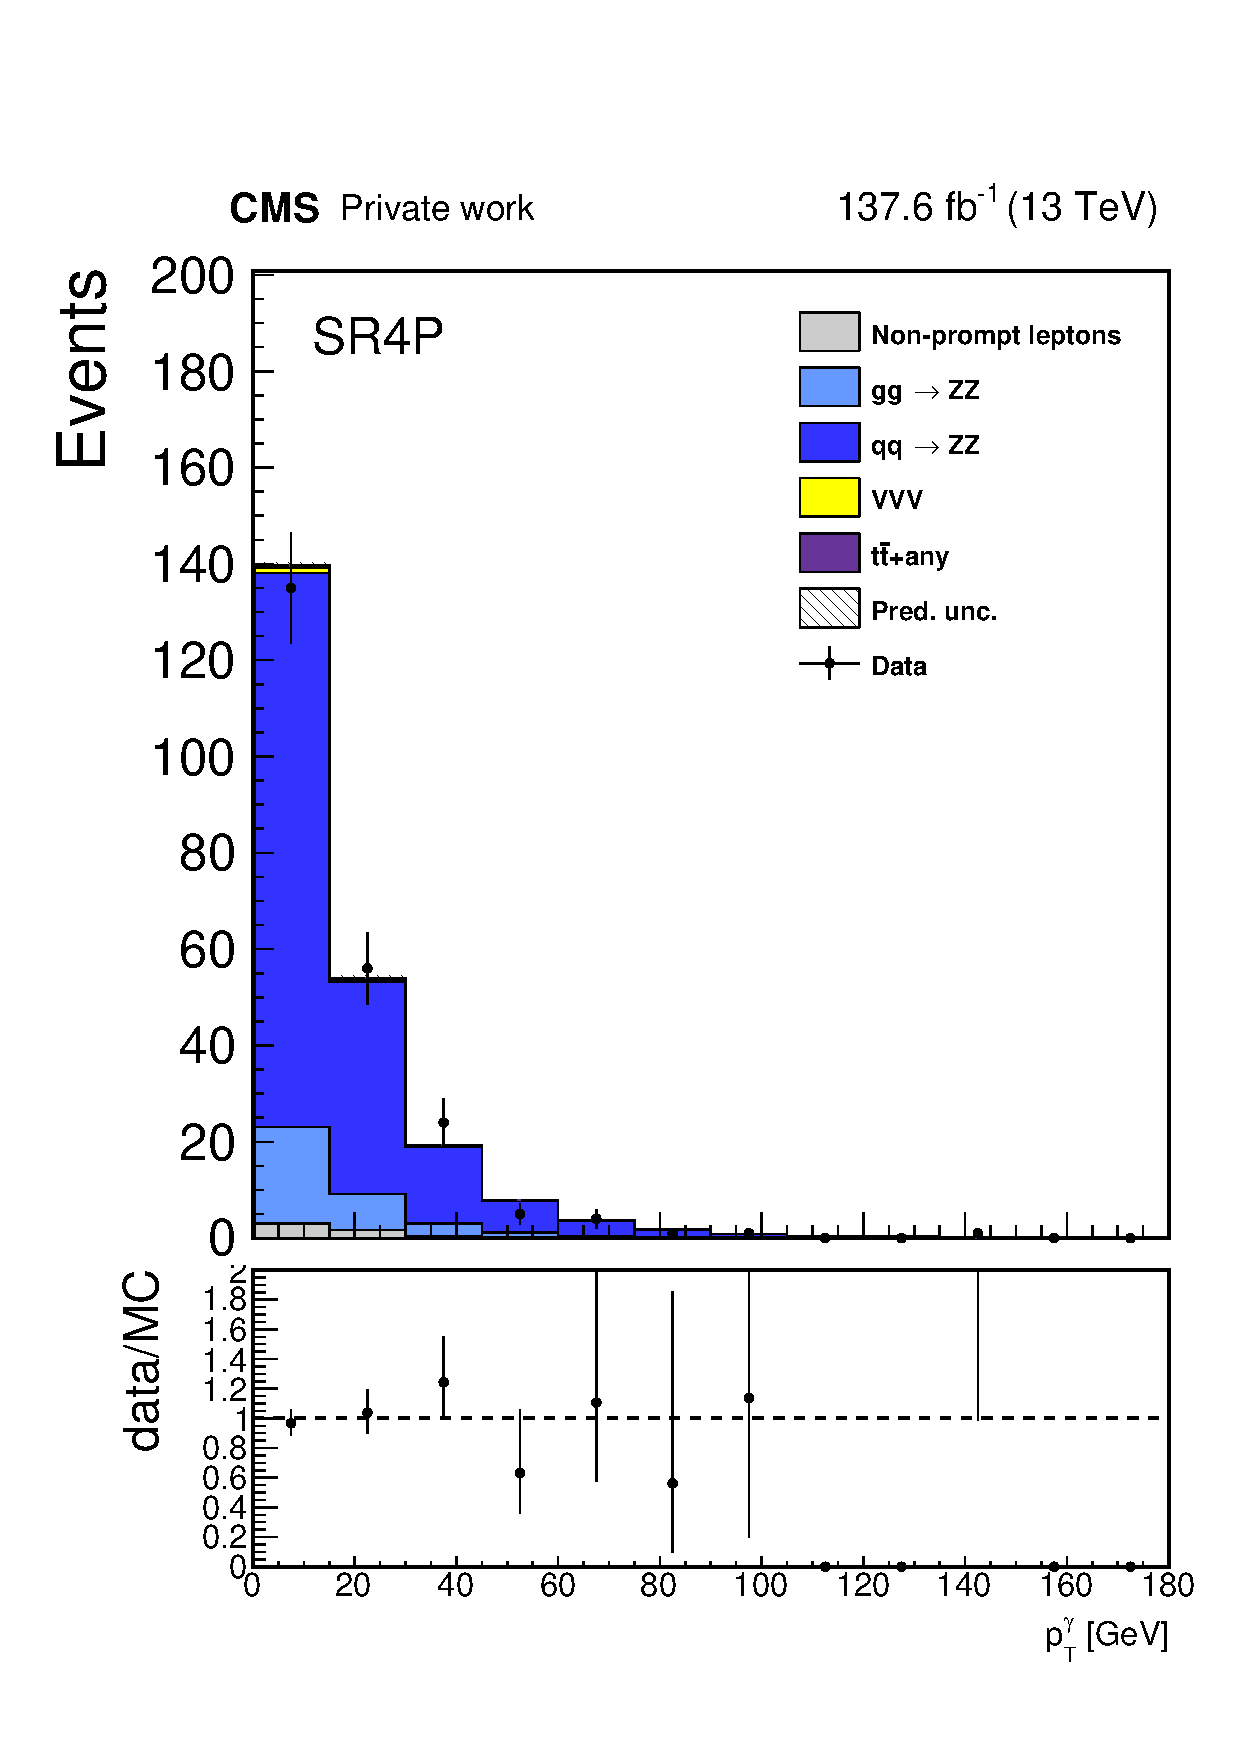
\includegraphics[width=.4\textwidth]{Figures/dataMC/Run2/lepCR/SR4P/lead_fsrPhotons_pt_pow.pdf}}
  \hfill
  \subfigure [Pseudorapidity]      {\includegraphics[width=.4\textwidth]{Figures/dataMC/Run2/lepCR/SR4P/lead_fsrPhotons_eta_pow.pdf}}
  \hfill\mbox{}
  \caption{Transverse momentum and pseudorapidity distributions of FSR photons associated to a lepton in the inclusive region with four charged leptons for \RunII.}
  \label{fig:distributions_fsrPhotons}
\end{figure}

%% \begin{figure}
%% \begin{center}
%%         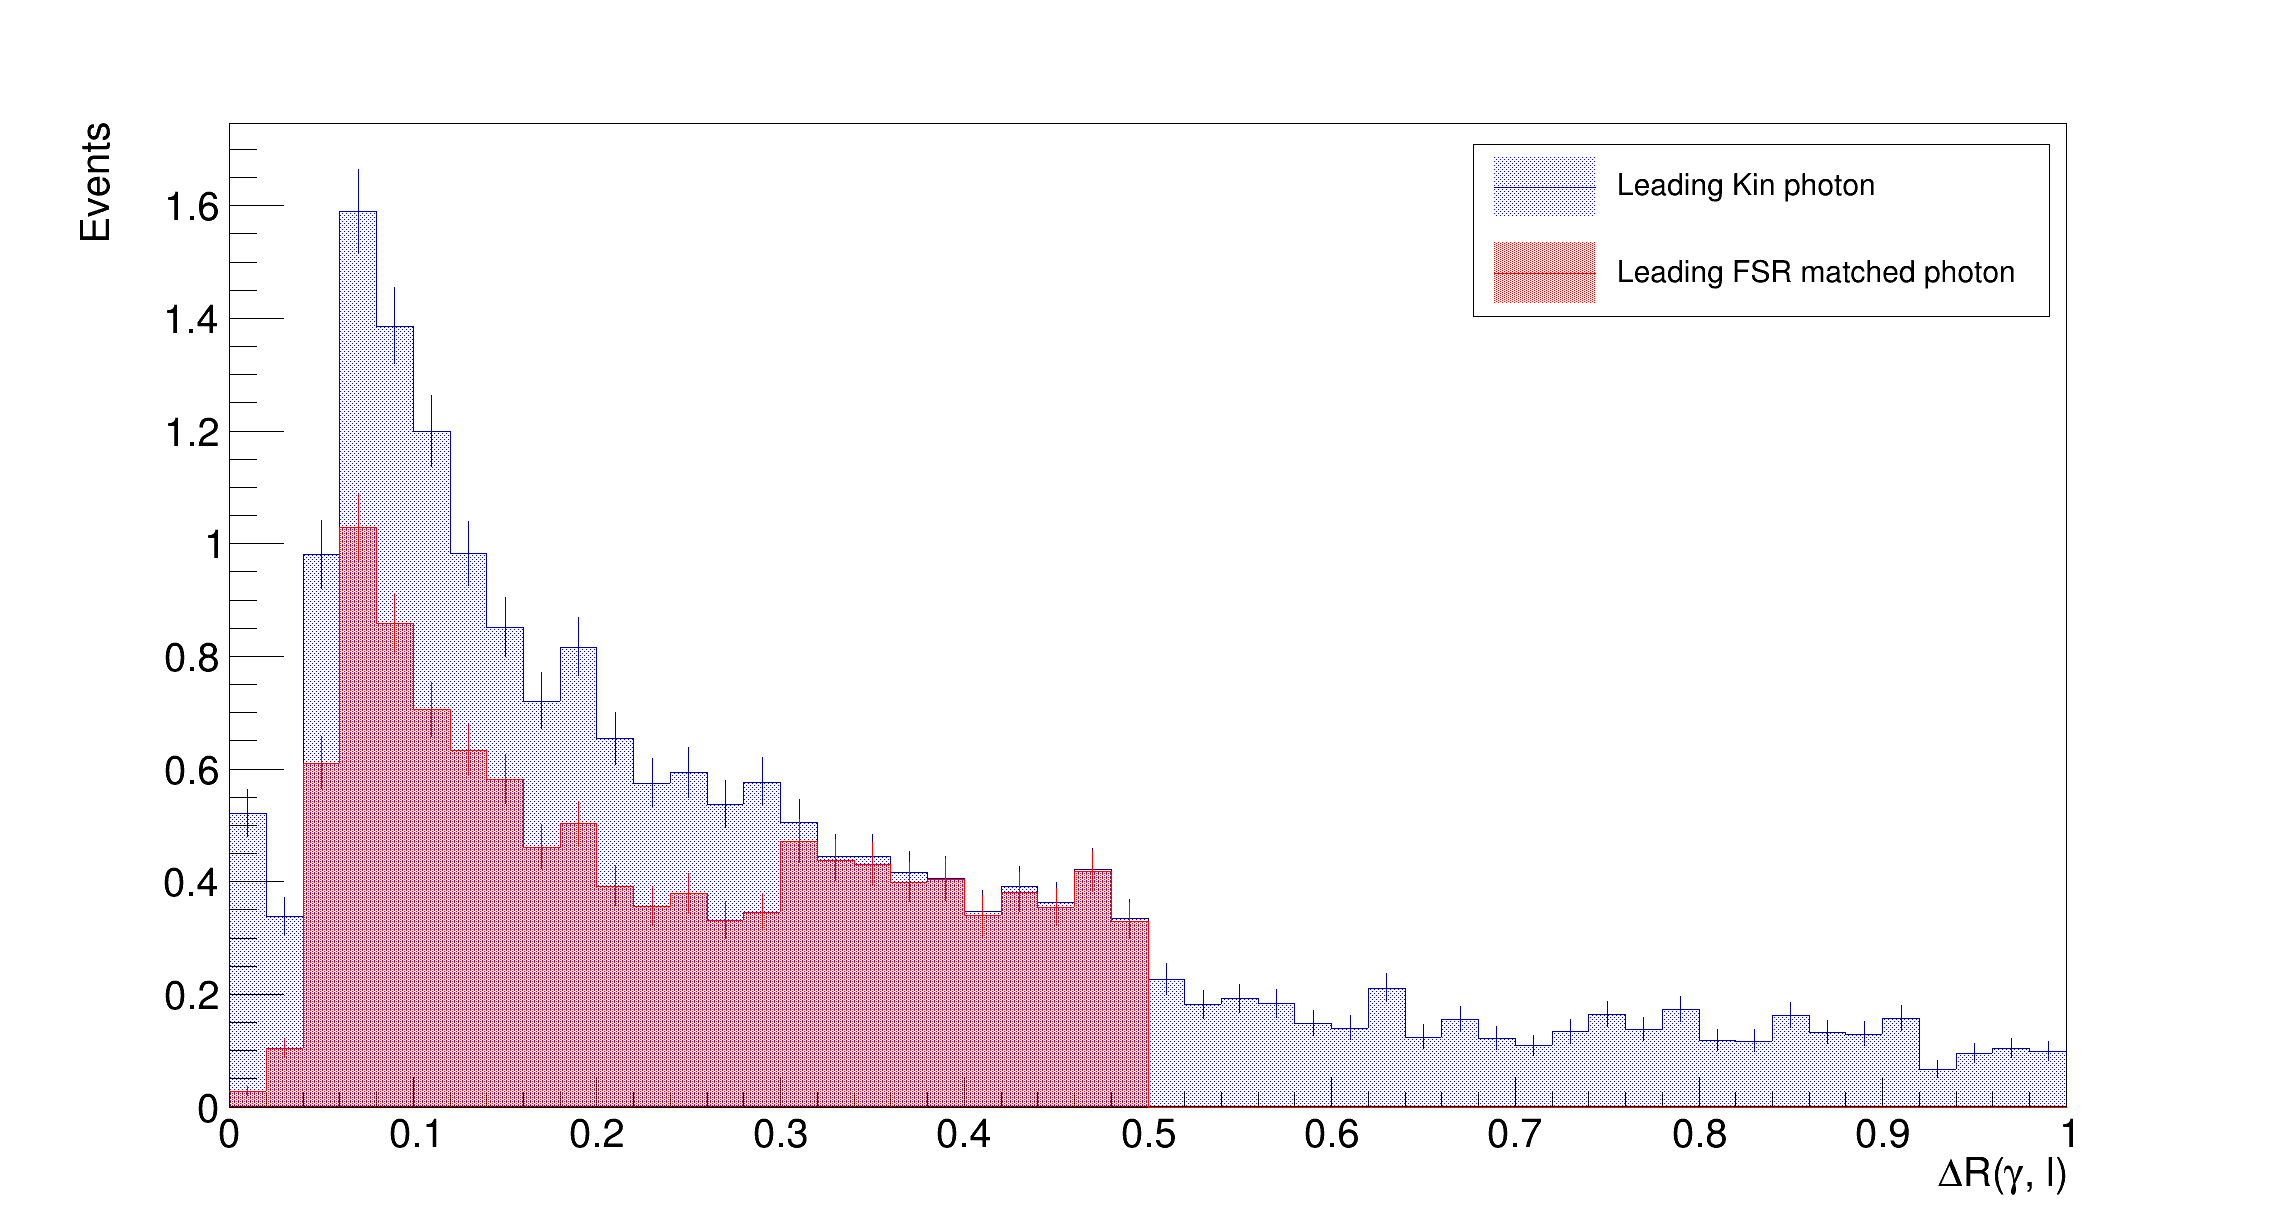
\includegraphics[width=0.8\textwidth]{Figures/lead_dRl_kin_vs_fsrMatched_rebinned.png}
%% \end{center}
%% \caption{$\Delta R(\ell, \gamma)$ for all the photons passing at least the `kinematic' selection with the $\Delta R$ cut relaxed, and for those selected as FSR in the ZZ$\gamma$ sample 2018.}
%% \label{fig:dRl_fsr_photons}
%% \end{figure}

% and the effect of not excluding FSR photons from the computation of the nonprompt rate


\subsection{Electrons}
\subsubsection{Isolation Optimisation}
\label{sec:eleiso}
The electron isolation is archieved through the use of the Particle Flow relative isolation,
which is defined as:
\begin{equation}
\text{RelPFiso} = (\sum_{\text{charged}} \ET + \sum^{\text{corr}}_{\text{neutral}} \ET)/\ET^{\,\Pe}
\label{eqn:elepfrelisoeqn}
\end{equation}
To mitigate the contribution from \pileup, only charged hadrons from the primary vertex are included,
while the corrected neutral component of isolation is then computed using the formula:
\begin{equation}
\label{eqn:neutralea}
  \sum^{\text{corr}}_{\text{neutral}} \ET = \text{max} \left(0,\, \sum^{\text{uncorr}}_{\text{neutral}} \ET + \sum_{\text{photons}} \ET - \ET^\text{PU} \right)
\end{equation}
The contribution from neutral \pileup{} is estimated using:
\begin{equation}
  \ET^{PU} =  \rho \times A_\text{eff}
\label{eqn:purho}
\end{equation}
where $\rho$ is the mean energy density, estimated as the median of the distribution of the transverse energy density per unit area of \pileup{} jets in the event, $\pt^\text{jet}/A_\text{jet}$,
while the effective area $A_{\text{eff}}$ is the geometric area of the isolation cone,
corrected by an $\eta$-dependent factor to account for the dependence of the \pileup{} energy density~\cite{CMS-EGM-13-001}.

%% was optimized in Ref.~\cite{AN-15-277} and the electron isolation working was
The threshold for the electron isolation,
calculated within a cone of radius $\DR = 0.3$
is chosen to be $\text{RelPFiso} < 0.35$. 

\subsubsection{Impact Parameter Selection}
\label{sec:eleSIP}
In order to ensure that the electron trajectories are consistent with a common primary vertex
they are required to have an associated track with a small impact parameter with respect to the event primary vertex.
The significance of the impact parameter (SIP) is used:
\begin{equation}
\label{eq:SIP3D}
\SIPthreeD \mathdefined \frac{|\rm IP_{3D}|}{\sigma_{\rm IP}} \ ,
\end{equation}
where ${\rm IP_{3D}}$ is the lepton impact parameter in three dimensions,
that is the distance with respect to the primary interaction vertex the point of closest approach,
and $\sigma_{\rm IP}$ the associated uncertainty.
Electrons for the analysis must satisfy $\SIPthreeD < 4$.

\subsubsection{Electron MVA}
\label{sec:eleMVA}
Reconstructed electrons are identified and isolated by means of a Gradient Boosted Decision Tree (GBDT) multivariate classifier algorithm,
which exploits observables from the electromagnetic cluster, the matching between the cluster and the electron track, observables based exclusively on tracking measurements as well as particle flow isolation sums.
It was developed for the $\PH \to \PZ \PZ^{*} \to 4 \Pl$ analysis~\cite{CMS-HIG-19-001}
and trained separately for each data taking year on a Drell-Yan plus jets MC sample.
The classifier is trained with the e\textbf{X}treme \textbf{G}radient \textbf{Boost}ing (XGBoost) optimized distributed gradient boosting library~\cite{Chen_2016}
designed to be highly efficient, flexible and portable.

% The MVA values are userFloat("ElectronMVAEstimatorRun2Summer16ULIdIsoValues"), and the cut is done in ZZAnalysis/AnalysisStep/plugins/EleFiller.cc
The full list of observables used can be found in the Table~\ref{tab:ele_ID_input_variables}.

\begin{table}[ht]
  \caption{Overview of input variables to the multivariate classifier used to identity electrons.}
  \label{tab:ele_ID_input_variables}
  \small
  \centering
  \resizebox{\textwidth}{!}{
  \begin{tabular}{c l}
    \toprule
    Observable type & Observable name \\
    \midrule
    \multirow{6}{*}{Cluster shape}
      & RMS of the energy-crystal number spectrum: $\sigma_{i\eta i\eta}$, $\sigma_{i\varphi i\varphi}$ \\
      & Super cluster width along $\eta$ and $\phi$ \\
      & Ratio of the hadronic energy behind the SC to the SC energy, $H/E$ \\
      & Circularity $(E_{5\times5} - E_{5\times1})/E_{5\times5}$ \\
      & Sum of the seed and adjacent crystal over the SC energy $R_{9}$ \\
      & For endcap training bins: energy fraction in pre-shower $E_\text{PS}/E_\text{raw}$ \\
    \hline
    \multirow{2}{*}{Track-cluster match}
      & Energy-momentum agreement $E_{tot}/p_{in}$, $E_{ele}/p_{out}$, $1/E_{tot} - 1/p_{in}$ \\
      & Position matching $\Delta\eta_{in}$, $\Delta\varphi_{in}$, $\Delta\eta_{seed}$ \\
    \hline
    \multirow{2}{*}{Tracking}
      & Fractional momentum loss $f_{brem} = 1 - p_{out}/p_{in}$ \\
      & Reduced $\chi^2$ of the KF and GSF track $\chi^{2}_{KF}$, $\chi^{2}_{\textrm{GSF}}$ \\
    \bottomrule
  \end{tabular}
  }
\end{table}


The model is trained on 2016, 2017, and 2018 Drell-Yan with jets MC sample for both signal and background. The separate training for three periods guarantees
optimal performance during the entire \RunII{} data taking period.


Tables~\ref{tab:ele_ID_WPA}, \ref{tab:ele_ID_WPB} and~\ref{tab:ele_ID_WPC} list the cuts values applied to the MVA output for 2016, 2017, 2018 training, respectively.
For 2018, the corresponding signal and background efficiencies are given as examples.
They are very similar for 2016 and 2017.

For the analysis, loose electrons have to pass this MVA identification and isolation working point.

\begin{table}
  \caption{Minimum BDT score required for passing the electron identification, for 2016 samples.}
  \label{tab:ele_ID_WPA}
  \centering
  \begin{tabular}{c c c c}
    \toprule    %----------------------------------------------------------------------------------------
    \pt range           & $|\eta| < 0.8$ & $0.8 < |\eta| < 1.479$ & $|\eta| > 1.479$ \\
    \midrule    %----------------------------------------------------------------------------------------
    $5 < \pt < 10 \GeV$ &  0.9503        &  0.9461                &  0.9387 \\
    $\pt > 10 \GeV$     &  0.3782        &  0.3587                & -0.5745 \\
    \bottomrule %----------------------------------------------------------------------------------------
  \end{tabular}
\end{table}

\begin{table}
  \caption{Minimum BDT score required for passing the electron identification, for 2017 samples.}
  \label{tab:ele_ID_WPB}
  \centering
  \begin{tabular}{c c c c}
    \toprule    %----------------------------------------------------------------------------------------
    \pt range           & $|\eta| < 0.8$ & $0.8 < |\eta| < 1.479$ & $|\eta| > 1.479$ \\
    \midrule    %----------------------------------------------------------------------------------------
    $5 < \pt < 10 \GeV$ &  0.8521        &  0.8268                &  0.8694 \\
    $\pt > 10 \GeV$     &  0.9825        &  0.9692                &  0.7935 \\
    \bottomrule %----------------------------------------------------------------------------------------
  \end{tabular}
\end{table}

\begin{table}
  \caption{Minimum BDT score required for passing the electron identification and corresponding signal and background efficiencies, for 2018 samples.}
  \label{tab:ele_ID_WPC}
  \centering
  \begin{tabular}{c c c c c}
    \toprule
    $|\eta|$ range                      & \pt range           & Cut on BDT & Signal eff. & Background eff. \\
    \midrule
    \multirow{2}{*}{$|\eta| < 0.8 $}    & $5 < \pt < 10 \GeV$ &  0.8956    &  81.0\,\%   &  4.4\,\% \\
                                        & $\pt > 10 \GeV$     &  0.0424    &  97.1\,\%   &  2.9\,\% \\
    \hline
    \multirow{2}{*}{$0.8<|\eta|<1.479$} & $5 < \pt < 10 \GeV$ &  0.9111    &  79.3\,\%   &  4.6\,\% \\
                                        & $\pt > 10 \GeV$     &  0.0047    &  96.3\,\%   &  3.6\,\% \\
    \hline
    \multirow{2}{*}{$|\eta| > 1.479$}   & $5 < \pt < 10 \GeV$ &  0.9401    & 73.0\,\%    &  3.6\,\% \\
                                        & $\pt > 10 \GeV$     & -0.6042    & 95.7\,\%    &  6.7\,\% \\
    \bottomrule
  \end{tabular}
\end{table}

\subsubsection{Analysis selection for electrons}%% {Electron Selection}
\label{sec:ele_selection}
Electron candidates are preselected using loose cuts on track-cluster matching observables, so as to preserve the highest possible efficiency while rejecting part of the QCD background. To be considered for the analysis, electrons are required to have a
transverse momentum $p^e_T >$ 7 GeV, a reconstructed $|\eta^e| <$ 2.5, and to satisfy a loose primary vertex
constraint defined as $d_{xy} < 0.5$ cm and $d_z < 1$ cm.
Such electrons are called {\bf loose electrons}.

The data-MC discrepancy is corrected using scale factors as is done for the electron selection with data efficiencies measured using the same tag-and-probe technique outlined later (see Section~\ref{sec:eleEffMeas}).
These studies for reconstructions are carried out by the EGM POG and the results are only summarised here.

The electron reconstruction scale factors
% are shown Fig.~\ref{fig:ele_rec_scale_factors} and
are applied as a function of the super cluster $\eta$ and electron $\pt$.


\subsection{Muons}
\subsubsection{Muon Isolation}
\label{sec:muoniso}
A Particle Flow based isolation is used to suppress the contamination from muon from hadronic decays inside jets.
The so-called $\Delta\beta$ correction is applied in order to subtract the \pileup{} contribution for the muons, 
whereby $\Delta\beta = \frac{1}{2} \sum^\text{charged had.}_\text{PU} \pt$
gives an estimate of the energy deposit of neutral particles (hadrons and photons) from \pileup{} vertices.

The relative isolation for muons is then defined as:
\begin{equation}
\text{RelPFIso} = \frac{1}{\pt^\text{muon}} \left( \sum_\text{charged had.} \pt + \max(0, \sum_\text{neutral had.} \ET + \sum_\text{photon} \ET - \Delta \beta) \right)
\label{eqn:mupfiso}
\end{equation}

where the sums run over the photons, charged and neutral hadrons in a cone with $\DR = 0.3$ around the muon.
Only charged hadrons originating from the primary vertex are included to minimise the \pileup{} contribution.

The isolation cone for muons was optimised and the working point was chosen to be $\text{RelPFiso}(\Delta R = 0.3) < 0.35$. 

Similarly to electrons, a condition on the significance of the 3D impact parameter (\SIPthreeD, see Equation \ref{eq:SIP3D}) is applied,
in order to ensure that muons are consistent with the primary vertex.
Muons are required to satisfy $\SIPthreeD < 4$.

\subsubsection{Muon Identification}
%More details on muon reconstruction can be found in Ref.~\cite{AN-15-277}.
The analysis definition of {\bf loose muons} requires
$p_T > 5$, $|\eta| < 2.4$, $dxy< 0.5$ cm, $dz < 1$ cm, where $dxy$ and $dz$ are 
defined w.r.t. the PV and using the 'muonBestTrack'. Muons have to be 
reconstructed by either the Global Muon or Tracker Muon algorithm. Standalone 
Muon tracks that are only reconstructed in the muon system are rejected.
Muons with \verb|muonBestTrackType==2| (standalone) are discarded even if they 
are marked as global or tracker muons. 

Loose muons with $\pt$ below 200\GeV that also pass
%Muon BDT (see below).
the PF loose muon ID are considered {\bf tight muons} for this analysis.
Note that the naming convention used for these IDs differs from the muon POG
naming scheme, in which the ``tight ID'' used here is called the ``loose ID''.

Those with $\pt$ above 200\GeV are considered tight if they pass
either the PF ID or the Tracker
High-$\pt$ ID, the definition of which is shown in Table~\ref{tab:highPtID}.
This relaxed definition is used to increase signal efficiency in the high
centre of mass energy regime.
% This relaxed definition is used to increase signal efficiency for the high-mass
% search. When a very heavy resonance decays to two $\cPZ$ bosons, both bosons
% will be very boosted.
In the lab frame, the leptons coming from the decay of
a highly boosted $\cPZ$ will be nearly collinear, and the PF ID loses 
efficiency for muons separated by approximately $\Delta R < 0.4$, which roughly 
corresponds to muons originating from $\cPZ$ bosons with $\pt > 500\GeV$.

\begin{table}[ht]
    \begin{small}
    \begin{center}
    \caption{
      The requirements for a muon to pass the Tracker High-$\pt$ ID. Note that
      these are equivalent to the Muon POG High-$\pt$ ID with the global track 
      requirements removed.
      }
    \begin{tabular}{|l|l|}
      \hline
      Plain-text description         & Technical description                 \\
      \hline
      Muon station matching          & Muon is matched to segments           \\
                                     & in at least two muon stations         \\
                                     & \textbf{NB: this implies the muon is} \\
                                     & \textbf{an arbitrated tracker muon.}  \\
      \hline                                                          
      Good $\pt$ measurement         & $\frac{\pt}{\sigma_{\pt}} < 0.3$      \\
      \hline
      Vertex compatibility ($x-y$)   & $d_{xy} < 2$~mm                       \\
      \hline
      Vertex compatibility ($z$)     & $d_{z} < 5$~mm                        \\
      \hline
      Pixel hits                     & At least one pixel hit                \\
      \hline
      Tracker hits                   & Hits in at least six tracker layers   \\
      \hline
    \end{tabular}
    \label{tab:highPtID}
    \end{center}
    \end{small}
\end{table}

An additional ``ghost-cleaning'' step is performed to deal with situations when a single muon
can be incorrectly reconstructed as two or more muons:

\begin{itemize}

\item Tracker Muons that are not Global Muons are required to be arbitrated.
\item If two muons are sharing 50\% or more of their segments then the muon with lower quality is removed.

\end{itemize}


Loose muons that pass also the identification, isolation and \SIPthreeD requirements are defined \textbf{tight muons}.

\subsection{Photon Identification}
\label{sec:photonID}
Photon candidates are required to have $E_{T} > 20 \GeV$ and be in the fiducial Barrel region or Endcap regions,
defined by $|\eta|<1.4442$ and $1.566<|\eta|<2.5$, respectively.
The photon candidates are also required to be separated from the closest lepton (electron or muon) by at least $\DR(\PGg, \Pl) > 0.5$,
which highly suppresses the contribution from FSR,
and is orthogonal to the selection used for lepton FSR recovery (see Section \ref{sec:FSRphotons}).

Different strategies are used to identify prompt (produced at the primary vertex) and isolated
electrons and photons, and separate them from background sources.
The most important background to prompt photons arises from jets fragmenting mainly into light neutral mesons
such as \Pgpz or \PGh, which promptly decay to two photons.
For the energy range of interest, the meson is significantly boosted, such that the two photons from the decay are nearly collinear
and are difficult to distinguish from a single-photon incident on the calorimeter.
%% Different working points are defined to identify either electrons or photons,
%% corresponding to identification efficiencies of approximately 70, 80, and 90 \%, respectively.
%% In all cases data and simulation efficiencies are compatible within 1-5 \% over the full $\eta$ and \ET ranges for electrons and photons.

Both a cut-based and a MVA-based ID are employed and compared in the analysis.
Each has its own advantages and disadvantages.
Due to its nature, the cut-based ID can be easily inverted by reversing only one or a few of its cuts.
On the other hand, MVA-based ID is more effective at discriminating between signal and background, providing a higher signal-to-noise ratio.

\paragraph{Identification variables\\}
One of the most efficient ways to reject photon backgrounds is the use of isolation energy sums,
a generic class of discriminating variables that are constructed from the sum of the reconstructed energy in a cone around photons in different subdetectors.
%% For this purpose, it is convenient to define cones in terms of an $\eta-\phi$ metric;
%% the distance with respect to the reconstructed photon direction is defined by \DR.
A veto region inside the cone is defined, to ensure that the energy from the photon itself is not included in this sum.

Photon isolation exploits the information provided by the PF event reconstruction (Section \ref{sec:ParticleFlow}).
The isolation variables are obtained by summing the transverse momenta of charged hadrons ($I_{ch}$), photons ($I_\PGg$), and neutral hadrons ($I_n$),
inside an isolation cone of $\DR = 0.3$ with respect to the electron or photon direction.
The larger the energy of the incoming electrons or photons, the larger the amount of energy spread around its direction in the various subdetectors.
For this reason, the thresholds applied on the isolation quantities are frequently parameterised as a function of the particle \ET.

The isolation variables are corrected to mitigate the contribution from pileup.
This contribution in the isolation region is estimated as $\rho A_{eff}$,
where $\rho$ is the median of the transverse energy density per unit area in the event
and $A_{eff}$ is the area of the isolation region weighted by a factor that accounts for the dependence of the pileup transverse energy density on the object $\eta$ \cite{CMS:electron-performance-2015}.
The quantity $\rho A_{eff}$ is subtracted from the isolation quantities.

The distributions of $I_\PGg$ before % after?
the $\rho$ corrections are shown in Figure~\ref{fig:Iph_CR2P2F} for photons in the EB and EE.

\begin{figure}
\subfigure [Barrel] {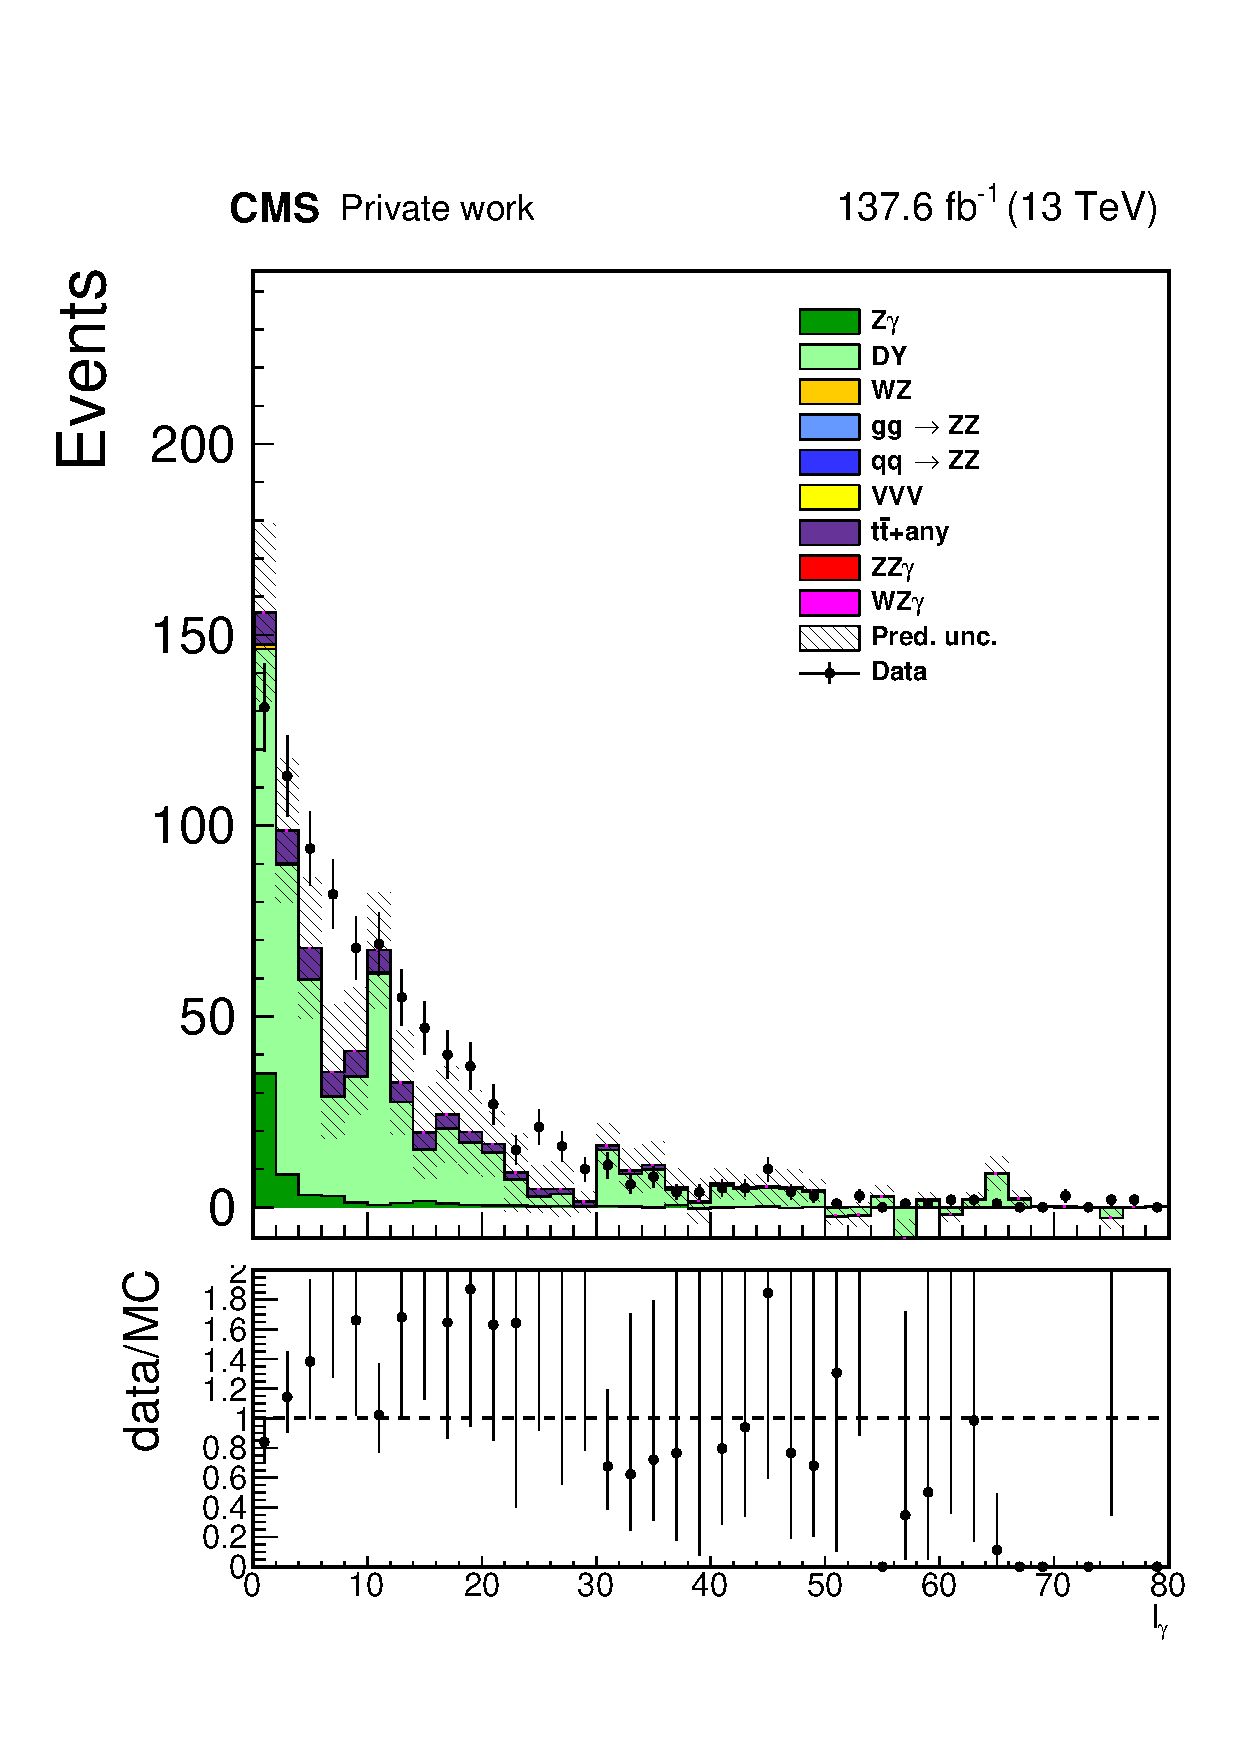
\includegraphics[width=.5\textwidth]{Figures/VVGammaAnalyzer_noLFR/Run2/fullMC/CR2P2F/kinPh_phIso_EB_pow.pdf}}%
\subfigure [Endcap] {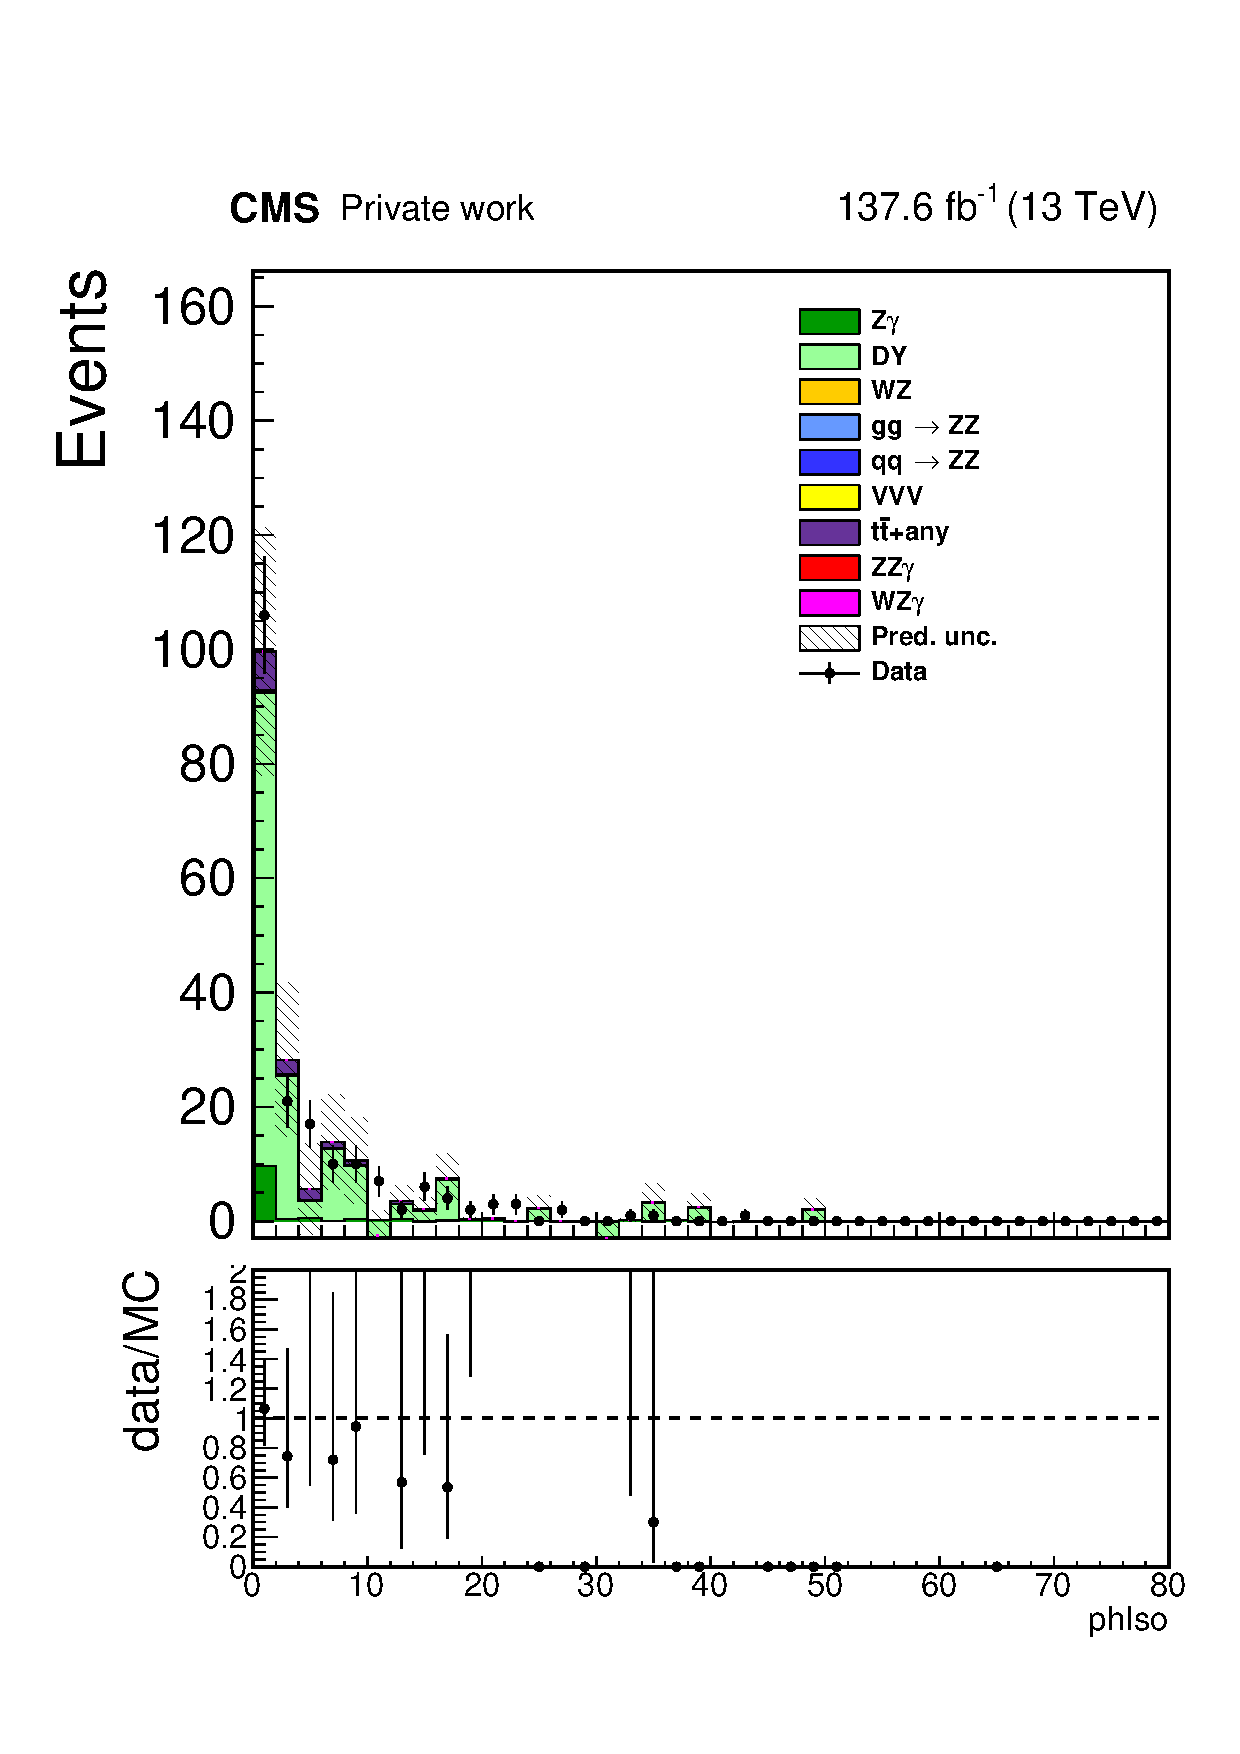
\includegraphics[width=.5\textwidth]{Figures/VVGammaAnalyzer_noLFR/Run2/fullMC/CR2P2F/kinPh_phIso_EE_pow.pdf}}
\caption{The PF photon isolation ($I_\PGg$), before the $\rho$ correction, in a cone defined by $\DR = 0.3$ for photons in the EB (left) and in the EE (right).
The events belong to the leptonic control region CR2P2F (see Section \ref{sec:fake_leptons}).
The lower panels display the ratio of the data to the simulation.}
\label{fig:Iph_CR2P2F}
\end{figure}

Another method to reject jets with high electromagnetic content exploits the shape of the electromagnetic shower in the ECAL.
Even if the two photons from neutral hadron decays inside a jet cannot be fully resolved, a wider shower profile is expected, on average,
compared with a single incident electron or photon.
This is particularly true along the $\eta$ axis of the cluster, since the presence of the material combined with the effect of the magnetic field
reduce the discriminating power resulting from the $\phi$ profile of the shower. 
In particular, the following two variables have high discriminating power.

The hadronic over electromagnetic energy ratio ($H/E$) is defined as the ratio between the energy deposited in the HCAL in a cone of radius $\DR = 0.15$
around the supercluster direction and the energy of the photon candidate.
\sieie, the second moment of the log-weighted distribution of crystal energies in $\eta$,
calculated in the $5 \times 5$ matrix around the most energetic crystal in the SC and rescaled to units of crystal size.
The mathematical expression is given below:
\begin{equation}
\label{eq:sieie}
\sieie \mathdefined \sqrt{ \frac{\sum_i^{5 \times 5} w_i(\eta_i - \bar{\eta}_{5 \times 5})}{\sum_i^{5 \times 5} w_i} }
\end{equation}
where $\eta_i$ is the pseudorapidity of the i-th crystal,
$\bar{\eta}_{5 \times 5}$ is the mean pseudorapidity of the $5 \times 5$ cells
and $w_i$ is a weight defined as $w_i = \mathrm{max}(0,\, 4.7 + \mathrm{ln}(E_i/E_{5 \times 5}))$,
which is nonzero if $E_i > 0.9\, \%\; E_{5 \times 5}$.
Looking at the numerator in Equation \ref{eq:sieie}, it is clear that \sieie is proportional to the distance between adjacent crystals,
which is 0.0175 in EB and varies from 0.0175 to 0.0 in EE.
Therefore, the spread of \sieie in EE is twice the one in EB.
The \sieie distribution is expected to be narrow for isolated electrons or photons, and broad for two-photon showers from meson decays.
The distributions of \sieie are shown in Figure \ref{fig:sieie_CR2P2F} for photons in the EB and EE.

\begin{figure}
\subfigure [Barrel] {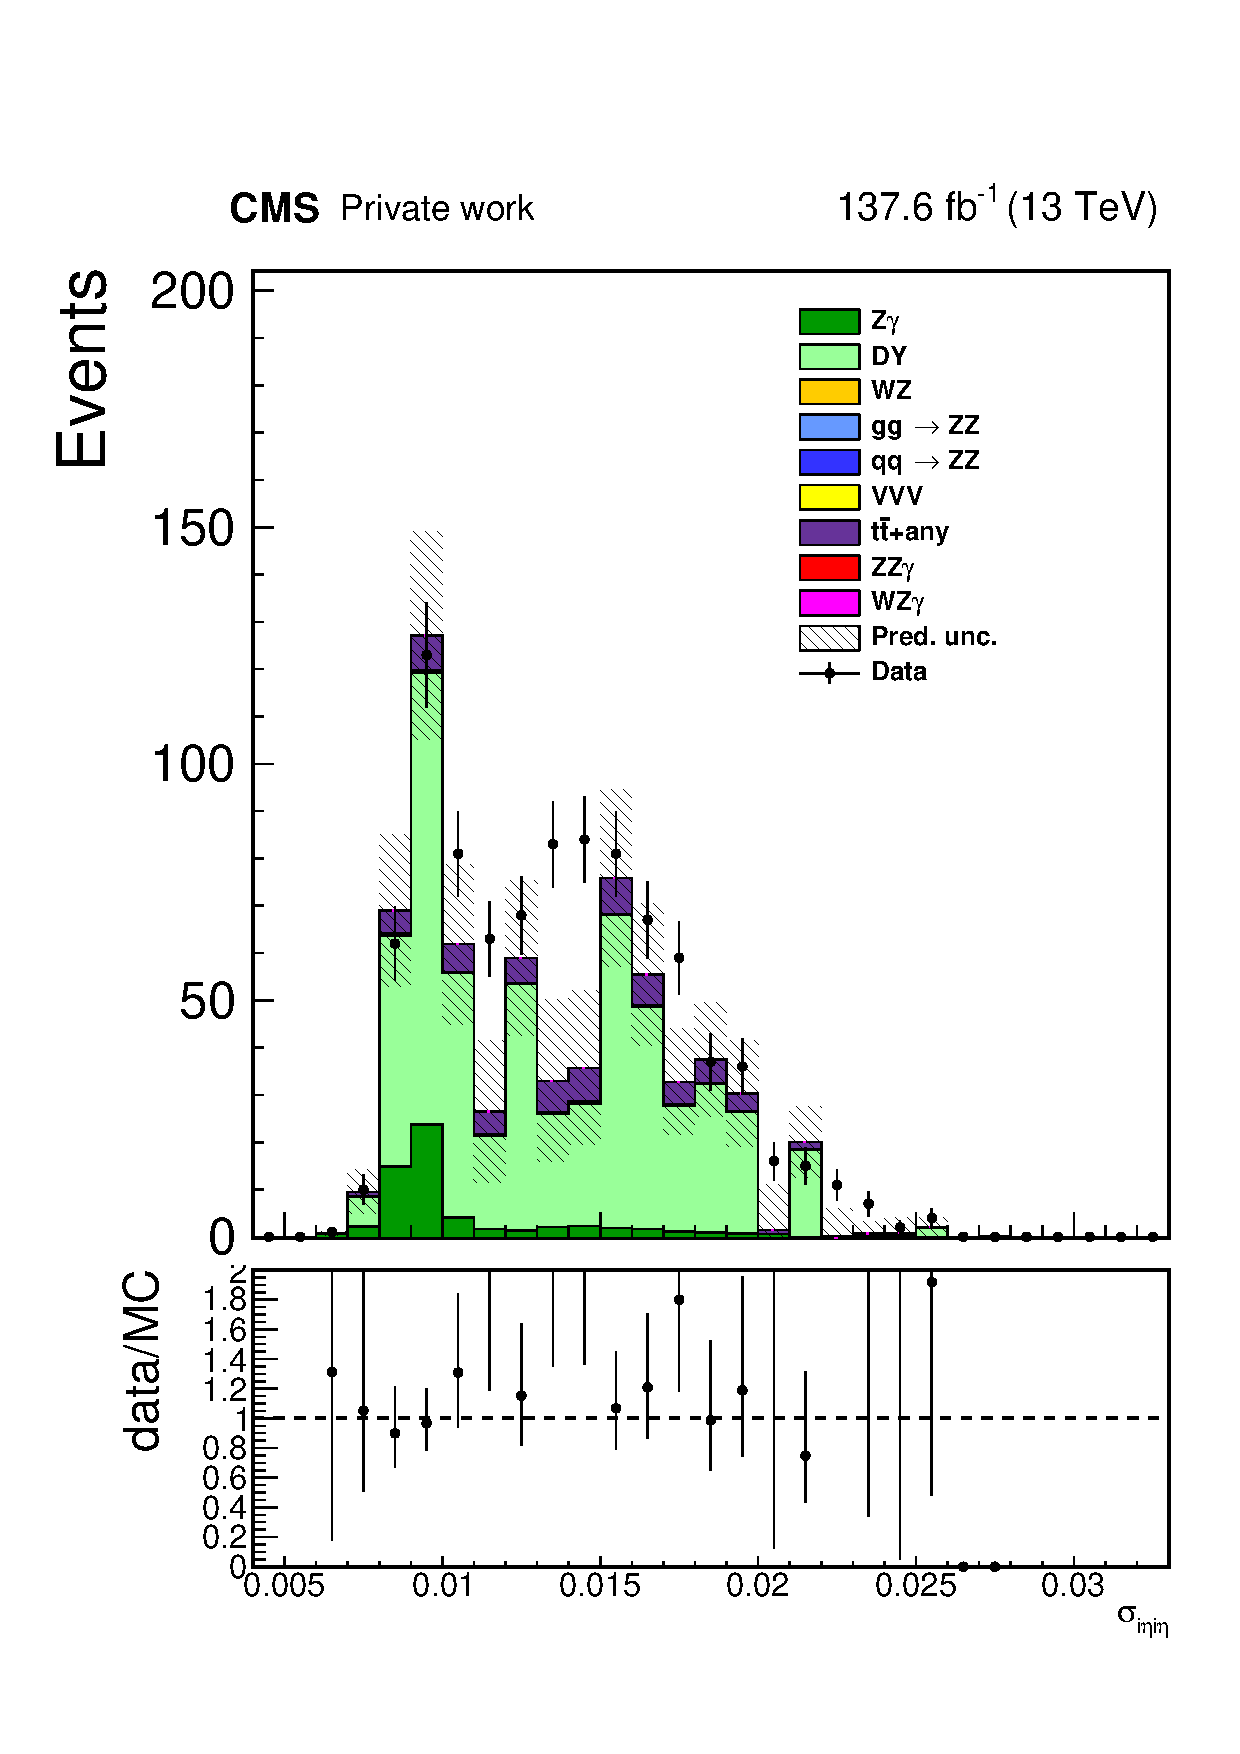
\includegraphics[width=.5\textwidth]{Figures/VVGammaAnalyzer_noLFR/Run2/fullMC/CR2P2F/kinPh_sieie_EB_pow.pdf}}%
\subfigure [Endcap] {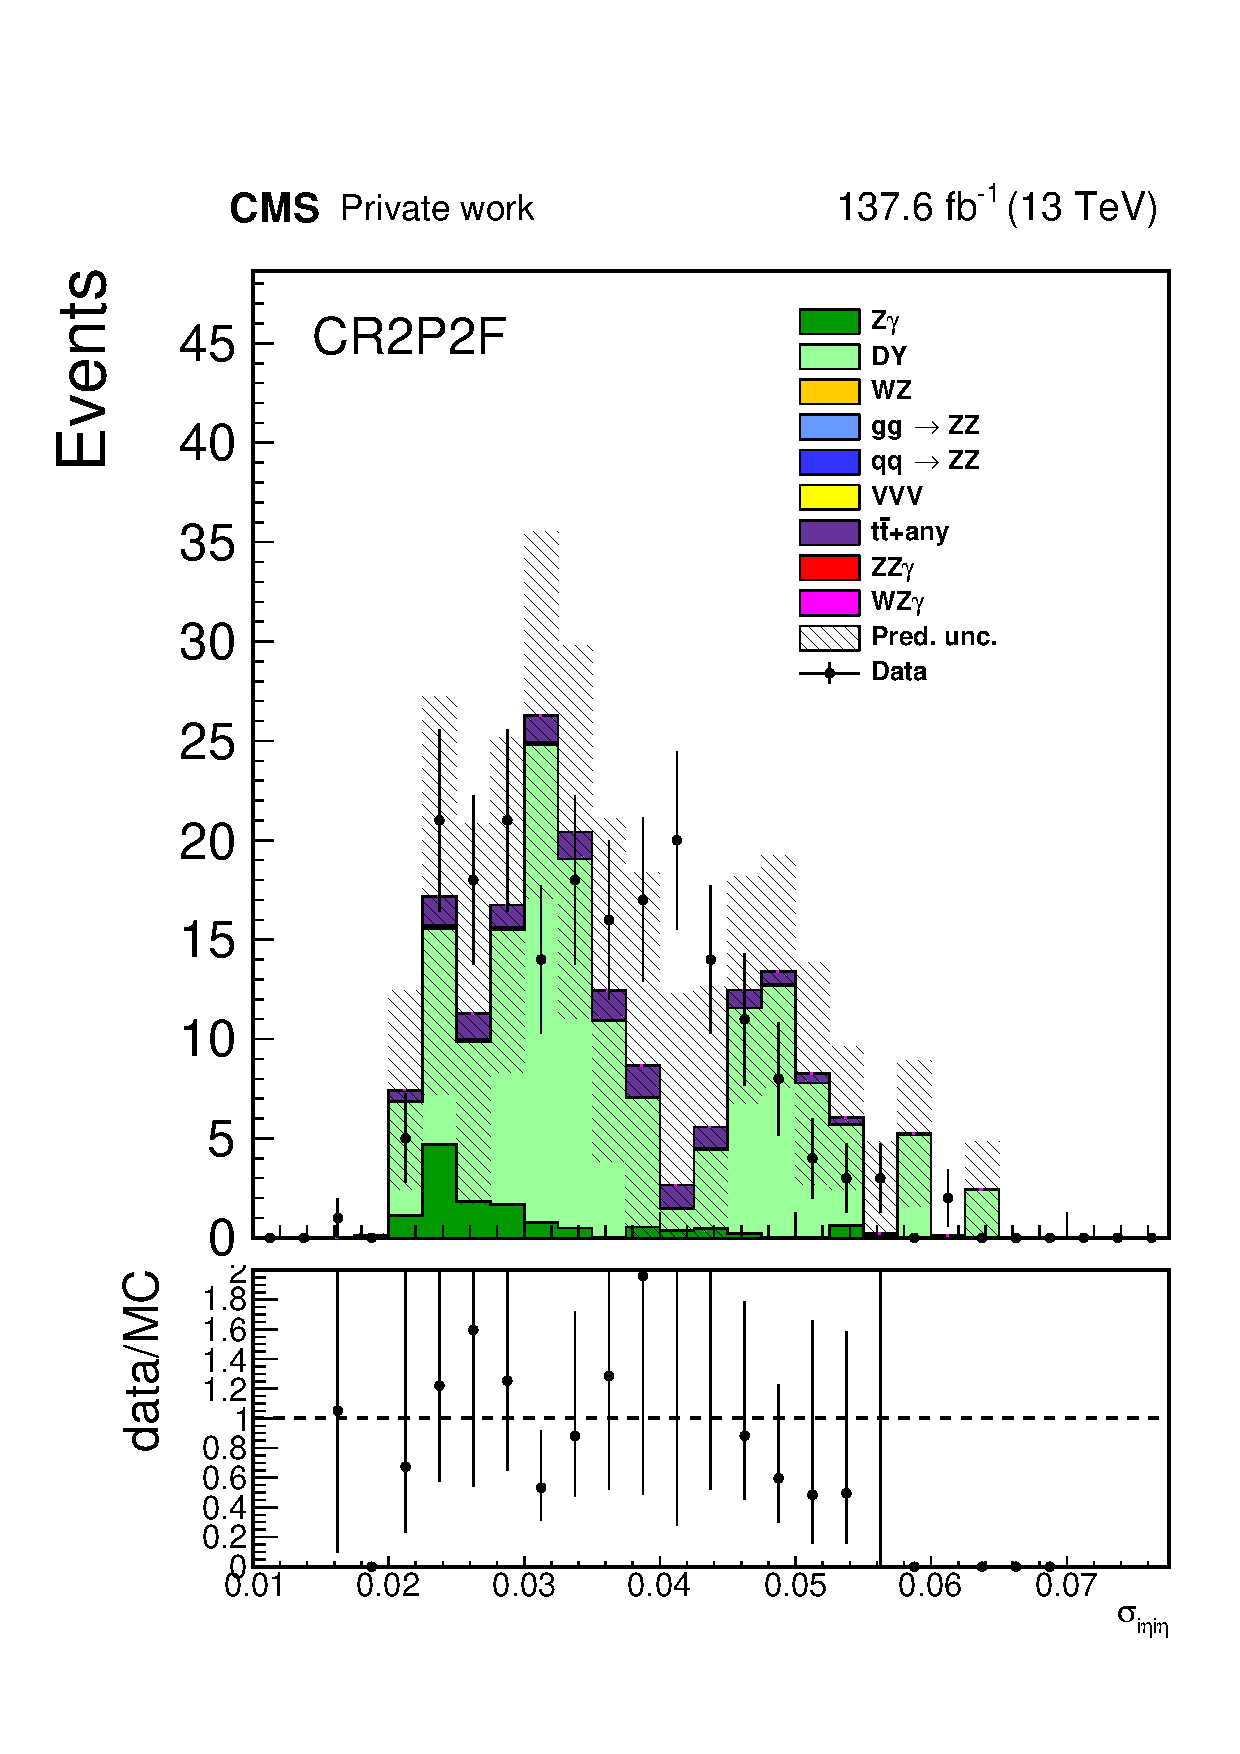
\includegraphics[width=.5\textwidth]{Figures/VVGammaAnalyzer_noLFR/Run2/fullMC/CR2P2F/kinPh_sieie_EE_pow.pdf}}
\caption{Distribution of \sieie for photons in the EB (left) and in the EE (right).
The events belong to the leptonic control region CR2P2F (see Section \ref{sec:fake_leptons}).
The lower panels display the ratio of the data to the simulation.}
\label{fig:sieie_CR2P2F}
\end{figure}

Another important variable is $R_9$, which is defined as the ratio between the energy contained in the $3 \times 3$ array of crystals,
centered around the most energetic crystal of the SC,
to the total energy of the supercluster.

\paragraph{Cut-based ID\\}
The cut-based photon ID~\cite{CMS:EGM-17-001} uses 5 variables: $H/E$, \sieie, $I_{ch}^{corr}$, $I_{n} ^{corr}$ and $I_{\PGg} ^{corr}$.
The Loose working point, shown in Table~\ref{tab:VPhotonID}, is selected for this analysis.
It provides 90\,\% efficiency on signal photons with 86\,\% (77\,\%) background rejection in the Barrel (Endcap).
The efficiency in data is well modelled in simulation, and the ratio between the two, shown in Figure \ref{fig:phEffSF}, is within 5\,\% from unity.
This ratio is referred as Scale Factor (SF), and is applied to simulation to correct for the residual mismodelling and avoid biasing the results.

\begin{table}
  \centering
  \renewcommand{\arraystretch}{1.4}
  \begin{tabular}{c c c}
    \toprule
    Variable                 &  Barrel $\quad |\eta| < 1.4442$     & Endcap $\quad 1.566 < |\eta| < 2.5$\\
    \midrule
    $H/E$                    & $0.04596$                           & $0.0590$                           \\
    $\sigma_{i\eta i\eta}$   & $0.0106$                            & $0.0272$                           \\
    $I_{ch}^{corr} [\GeV]$   & $1.694$                             & $2.089$                            \\
    $I_{n} ^{corr} [\GeV]$   & \renewcommand{\arraystretch}{1}\begin{tabular}{c} $24.032 + 0.01512\, p_{T}^{\gamma} +$\\$+ 2.259 \cdot 10^{-5}\, (p_{T}^{\gamma})^2$ \end{tabular}
                             & \renewcommand{\arraystretch}{1}\begin{tabular}{c} $19.722 + 0.0117\, p_{T}^{\gamma} +$ \\$+ 2.3 \cdot 10^{-5}\, (p_{T}^{\gamma})^2$   \end{tabular}\\
    $I_{\PGg}^{corr} [\GeV]$ & $2.876 + 0.004017\, p_{T}^{\gamma}$ & $4.162 + 0.0037\, p_{T}^{\gamma}$  \\
    \bottomrule
  \end{tabular}
  \caption[.]{Cut thresholds of the Loose working point cut-based photon ID.}
  \label{tab:VPhotonID}
\end{table}

\begin{figure}
  \subfigure [2016preVFP ] {\resizebox{.5\textwidth}{!}{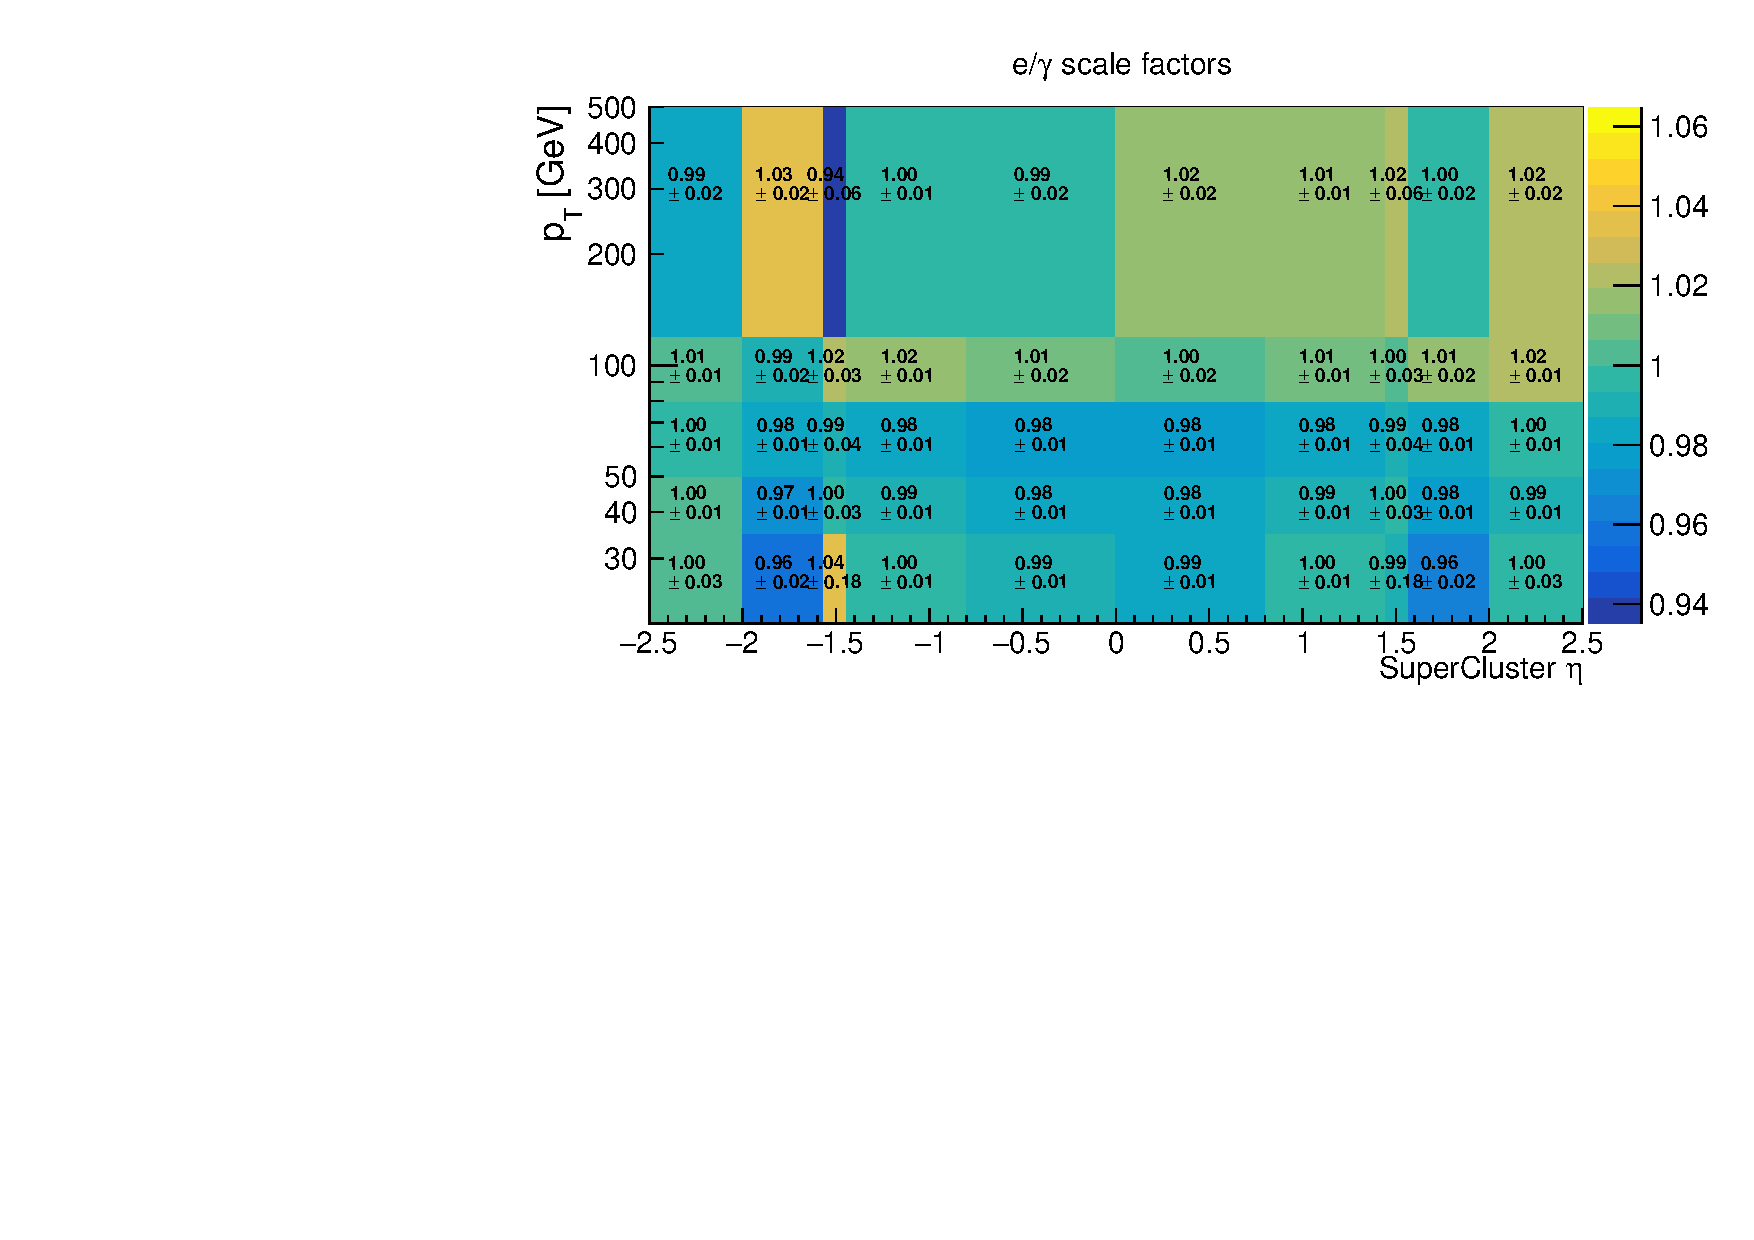
\includegraphics[width=.5\textwidth]{SF/phEffSF_2016preVFP.pdf} }}
  \subfigure [2016postVFP] {\resizebox{.5\textwidth}{!}{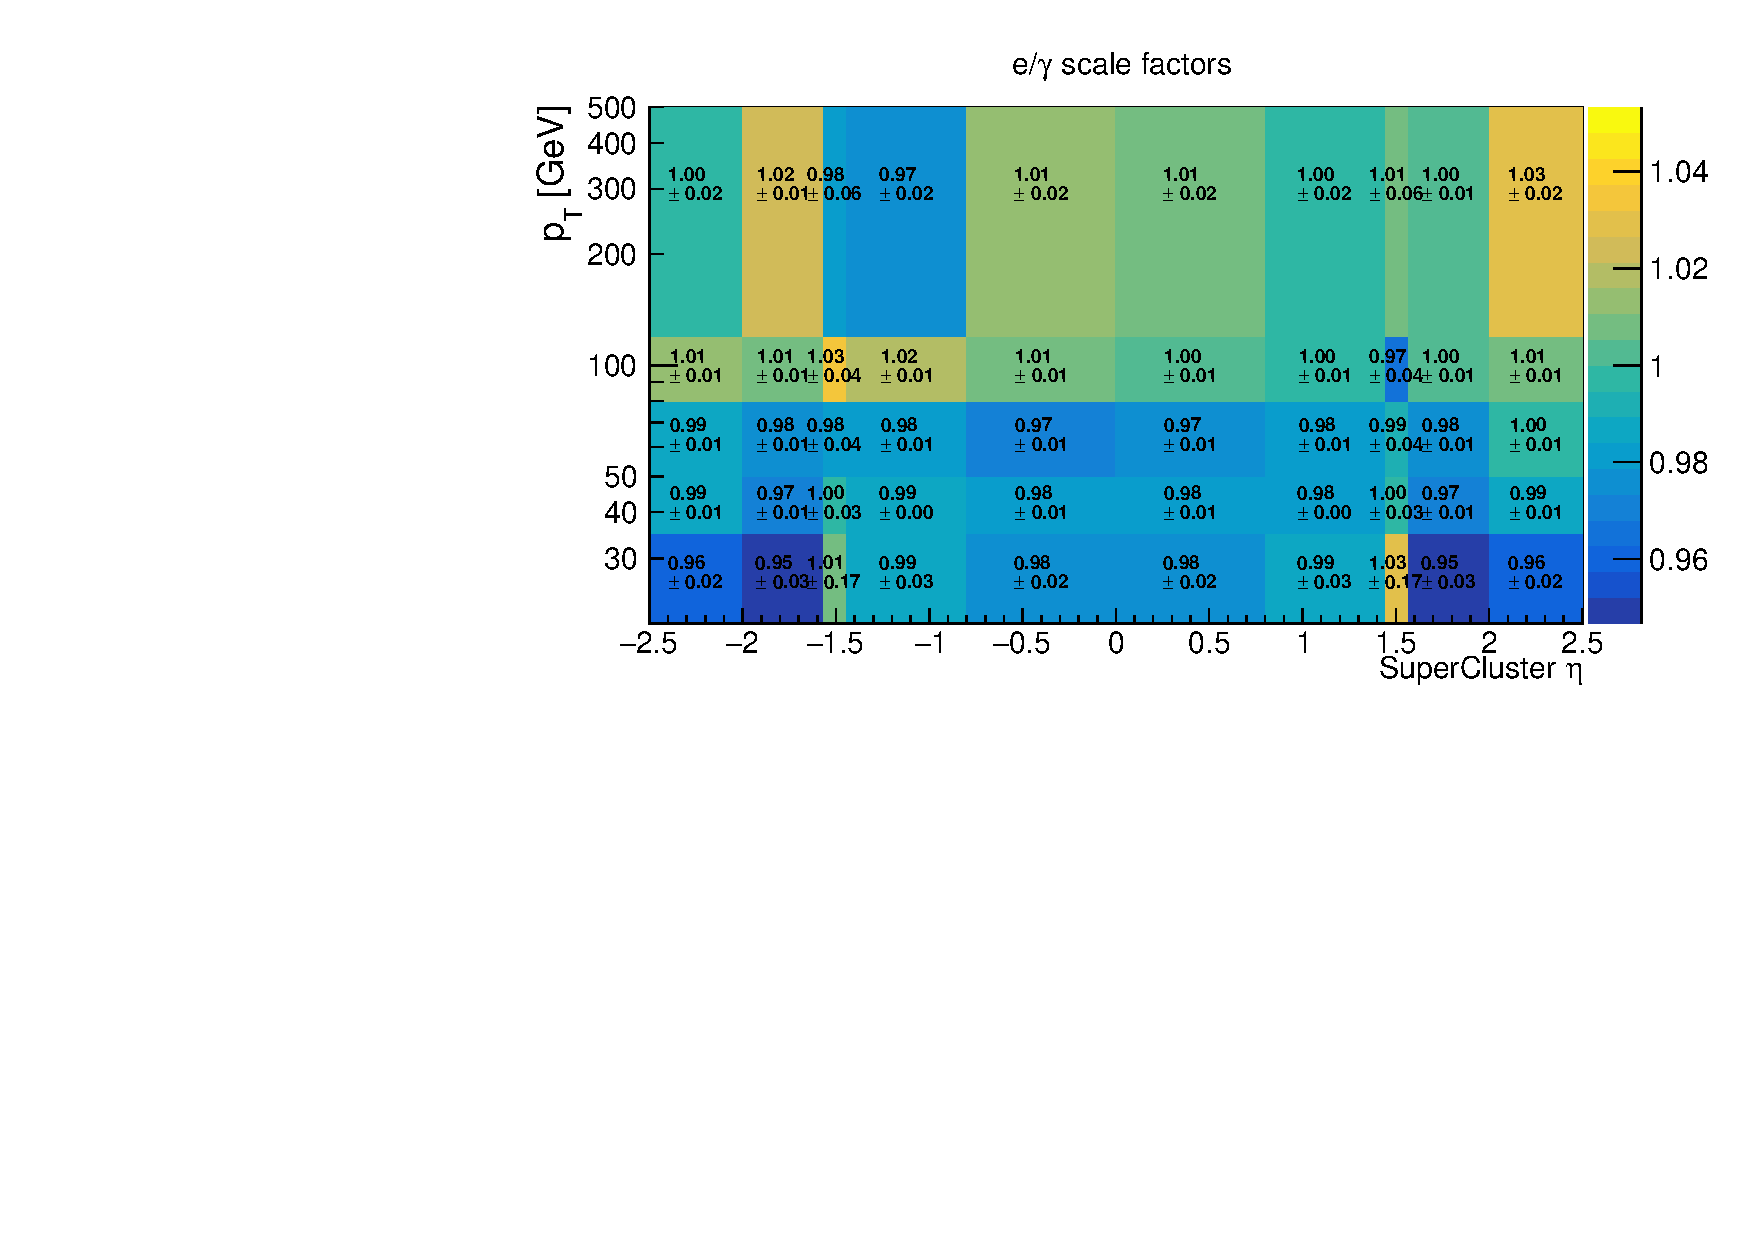
\includegraphics[width=.5\textwidth]{SF/phEffSF_2016postVFP.pdf}}}\\
  \subfigure [2017]        {\resizebox{.5\textwidth}{!}{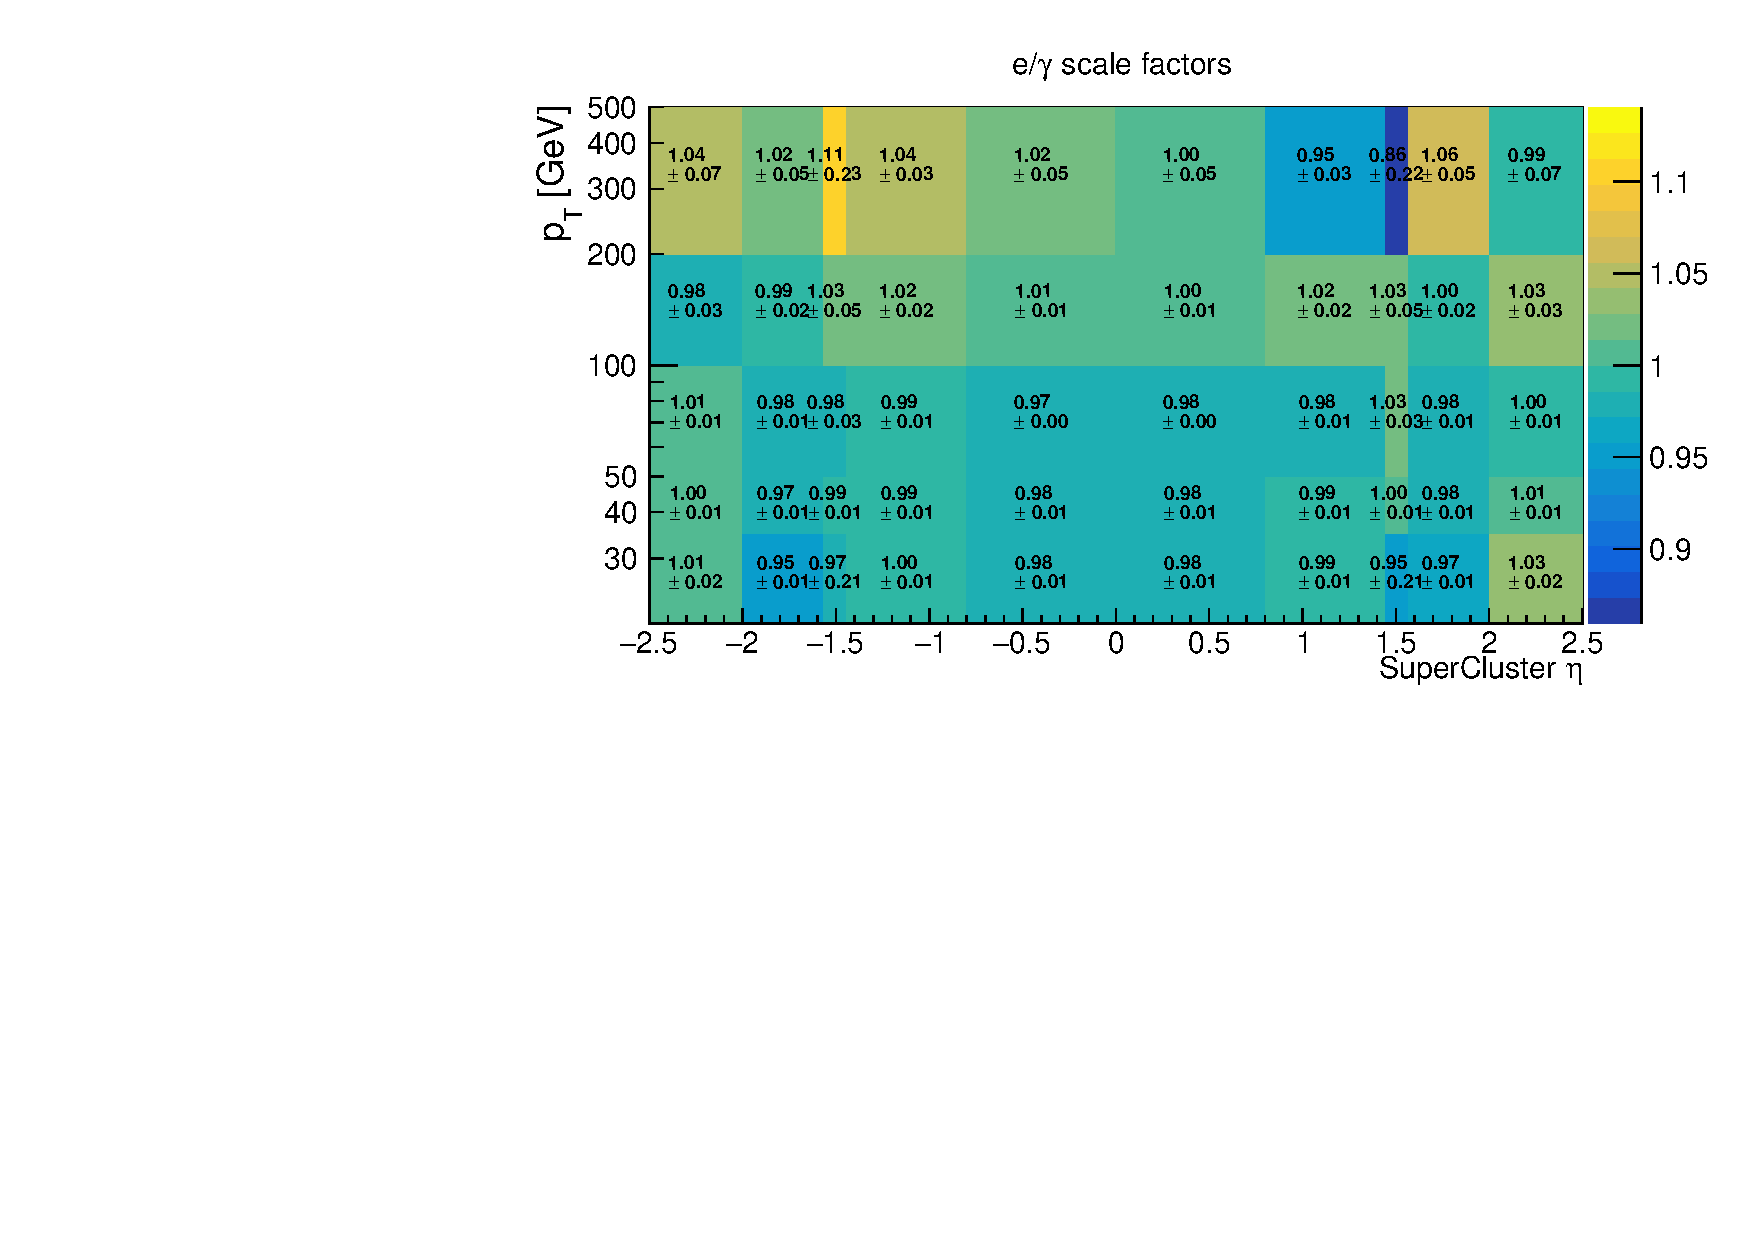
\includegraphics[width=.5\textwidth]{SF/phEffSF_2017.pdf}}}
  \subfigure [2018]        {\resizebox{.5\textwidth}{!}{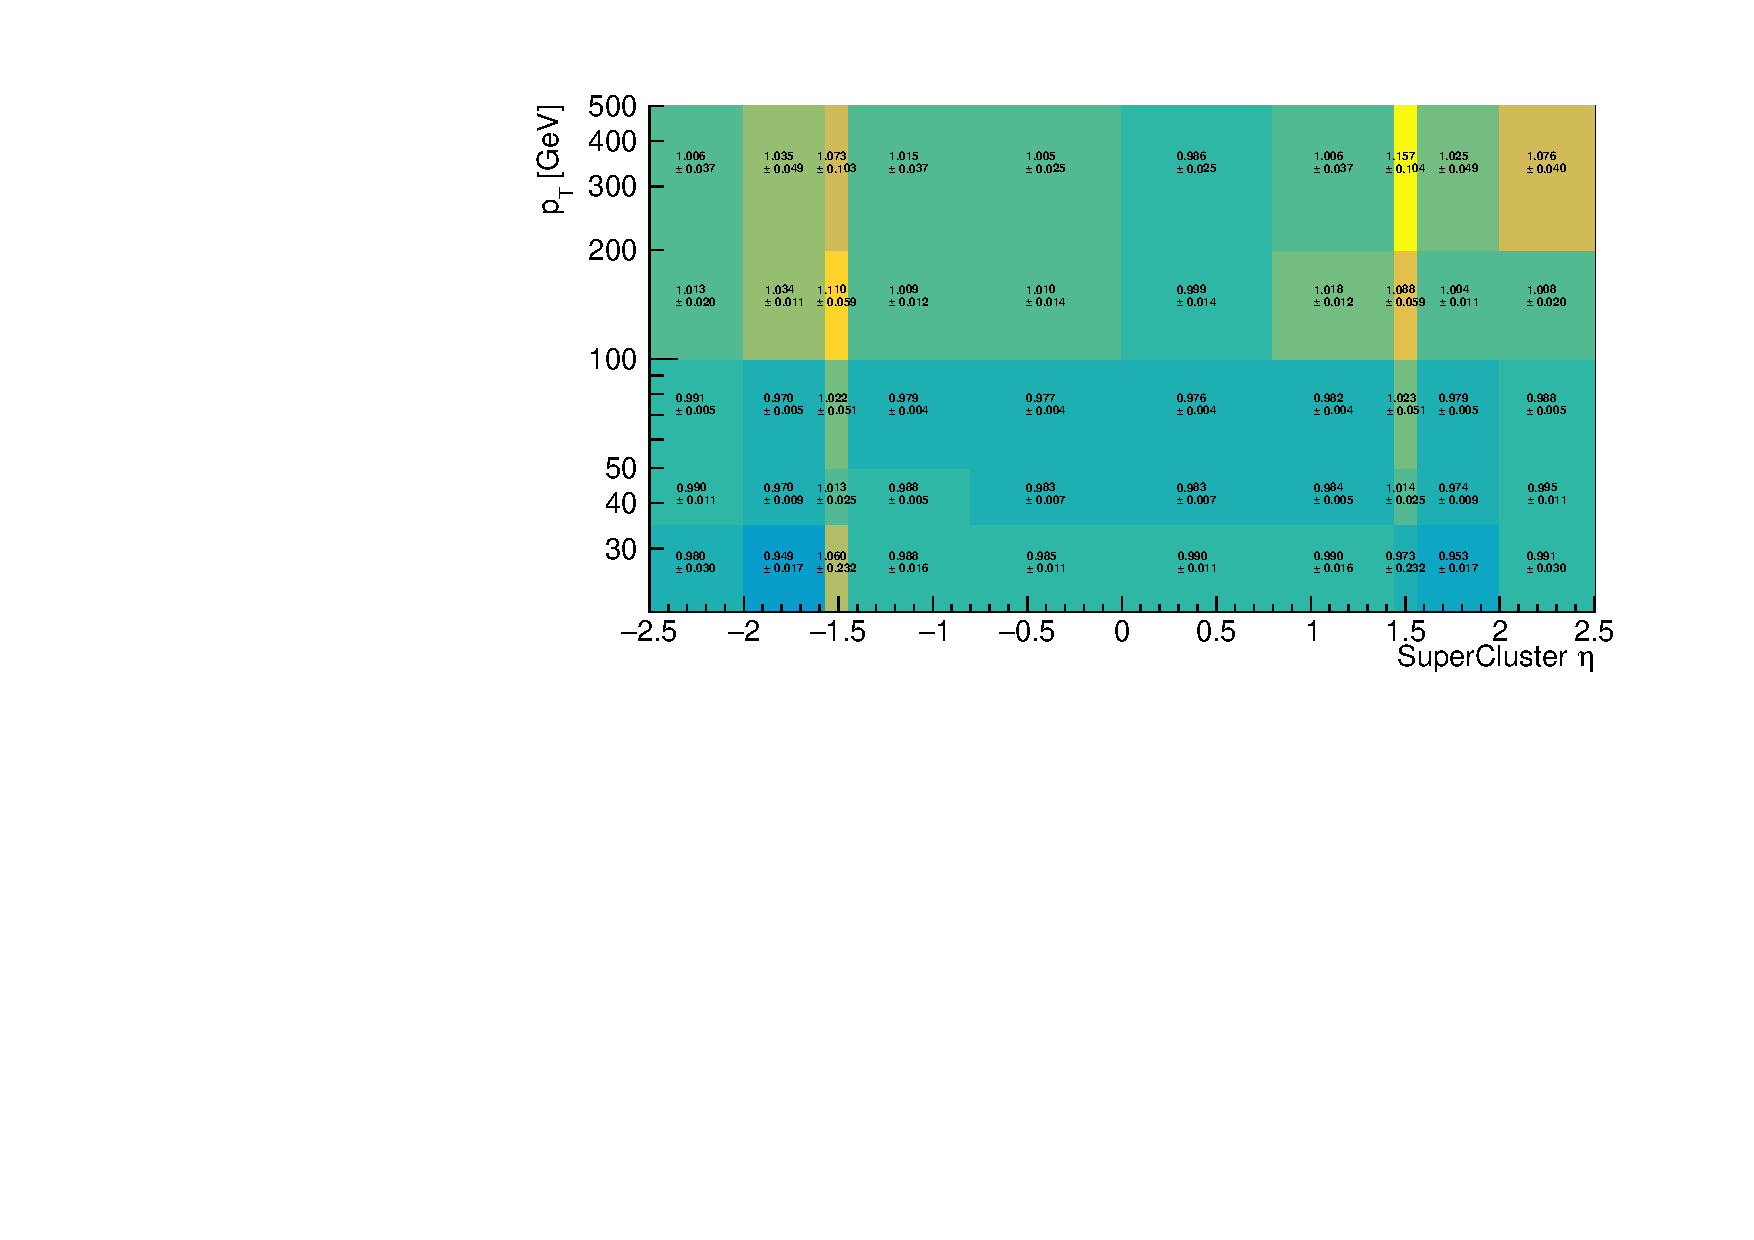
\includegraphics[width=.5\textwidth]{SF/phEffSF_2018.pdf}}}
  \caption{Photon efficiency scale factors for the cut-based Loose ID.}
  \label{fig:phEffSF}
\end{figure}

Besides the identification working points, an electron veto selection (CSEV veto) is also applied.
%% The scale factors are shown in ~\ref{tab:eleveto_SFs}.

%% \begin{table}[htbp]
%%  \centering
%%    \begin{tabular}{|c|c|l|l|}
%%    \hline
%%    Year & $p_T$& barrel & endcap\\ \hline
%%    2016 & inclusive &0.9938 $\pm$ 0.0119 & 0.9875 $\pm$ 0.0044\\\hline
%%    2017 & inclusive & 0.9862 $\pm$ 0.0030 & 0.9638 $\pm$ 0.0047\\\hline
%%    \multirow{3}{*}{2018} &10 GeV$<p_{T}^{\gamma}<30$ GeV &0.9869 $\pm$ 0.0043& 0.9535 $\pm$ 0.0054\\
%%    & 30 GeV$<p_{T}^{\gamma}<$60 GeV  &0.9908  $\pm$ 0.0111 & 0.9646 $\pm$ 0.0076\\
%%    & 60 GeV$<p_{T}^{\gamma}<$200 GeV &1.0084  $\pm$ 0.0856& 1.0218 $\pm$ 0.1178\\
%%    \hline
%%    \end{tabular}
%%    \caption{Electron veto scale factors for barrel and endcap corresponding to 2016 to 2018.}
%%    \label{tab:eleveto_SFs}
%%  \end{table}

%\begin{figure}[b]
%  \begin{center}
%    \includegraphics[width=0.8\textwidth]{figs/photon_SFs.pdf}
%    \caption{Photon ID scale factors for cut-based loose Photon selection}
%    \label{fig:PhotonEff}
%  \end{center}
%\end{figure}

\paragraph{Multivariate ID\\}
A more sophisticated photon identification strategy, is based on a multivariate technique, based on a Boosted Decision Tree (BDT) \cite{CMS:EGM-17-001}.
This multivariate (MVA) discriminant is built based on 14 input variables,
and provides excellent separation between signal (prompt photons) and background from misidentified jets.
The signal is defined as reconstructed photons from a \PGg + jets simulated sample that are matched at generator level with prompt photons within a cone of size $\DR = 0.1$,
whereas the background is defined by reconstructed photons in the same sample that do not match with a generated photon.
Photon candidates with $\ET > 15 \GeV$, $|\eta| < 2.5$, and satisfying very loose preselection requirements are used for the training of the BDT.
The variables used include the energy and shower shape of the supercluster, as well as various isolations.
Some of these variables are also employed by the cut-based ID, so the two discriminants are not independent.
%% The full list is shown in Table~\ref{tab:MVAvariables}.
%% The version used is \texttt{RunIIFall17v2}.

%% \begin{table}[ht]
%% \caption[.]{Variables used by the MVA-based ID, version \texttt{RunIIFall17v2}}
%% \label{tab:MVAvariables}
%% \centering
%% \begin{tabular}{l|l}
%% Name & variable\\
%% \hline
%% SCRawE             & superCluster.rawEnergy                                               \\
%% r9                 & r9                                                                   \\
%% sigmaIetaIeta      & full5x5\_showerShapeVariables.sigmaIetaIeta                          \\
%% etaWidth           & superCluster.etaWidth                                                \\
%% phiWidth           & superCluster.phiWidth                                                \\
%% covIEtaIPhi        & full5x5\_showerShapeVariables.sigmaIetaIphi                          \\
%% s4                 & full5x5\_showerShapeVariables.e2x2/full5x5\_showerShapeVariables.e5x5\\
%% scEta              & superCluster.eta                                                     \\
%% rho                & fixedGridRhoAll                                                      \\
%% esEffSigmaRR       & full5x5\_showerShapeVariables.effSigmaRR                             \\
%% esEnergyOverRawE   & superCluster.preshowerEnergy/superCluster.rawEnergy                  \\
%% phoIso03           & photonIso                                                            \\
%% chgIsoWrtChosenVtx & chargedHadronIso                                                     \\
%% chgIsoWrtWorstVtx  & chargedHadronWorstVtxIso                                             \\
%% \end{tabular}
%% \end{table}

Two working points are provided centrally by the the dedicated group within CMS:
\texttt{wp90} and \texttt{wp80}, corresponding to 90 \% and 80 \% prompt photon efficiency respectively.
The cuts on the MVA estimator value that define the two working points are detailed in Table~\ref{tab:MVAwpCuts}.

\begin{table}[ht]
\caption[.]{Working points of the photon MVA-based ID, version \texttt{RunIIFall17v2}}
\label{tab:MVAwpCuts}
\centering
\begin{tabular}{lrr}
\toprule
Name & Barrel & Endcap \\
\midrule
\texttt{wp80} & -0.02 & -0.26 \\
\texttt{wp90} &  0.42 &  0.14 \\
\bottomrule
\end{tabular}
\end{table}

As with any other ID, to account for difference in the modelling of its efficiency in simulations and the true efficiency in data,
Scale Factors are measured for each year in different bins of \pt and $\eta$ for \texttt{wp80} (Figure \ref{fig:phEffMVASF_wp80}) and \texttt{wp90} (Figure \ref{fig:phEffMVASF_wp90}).

\begin{figure}
\centering
\subfigure [2016preVFP ] {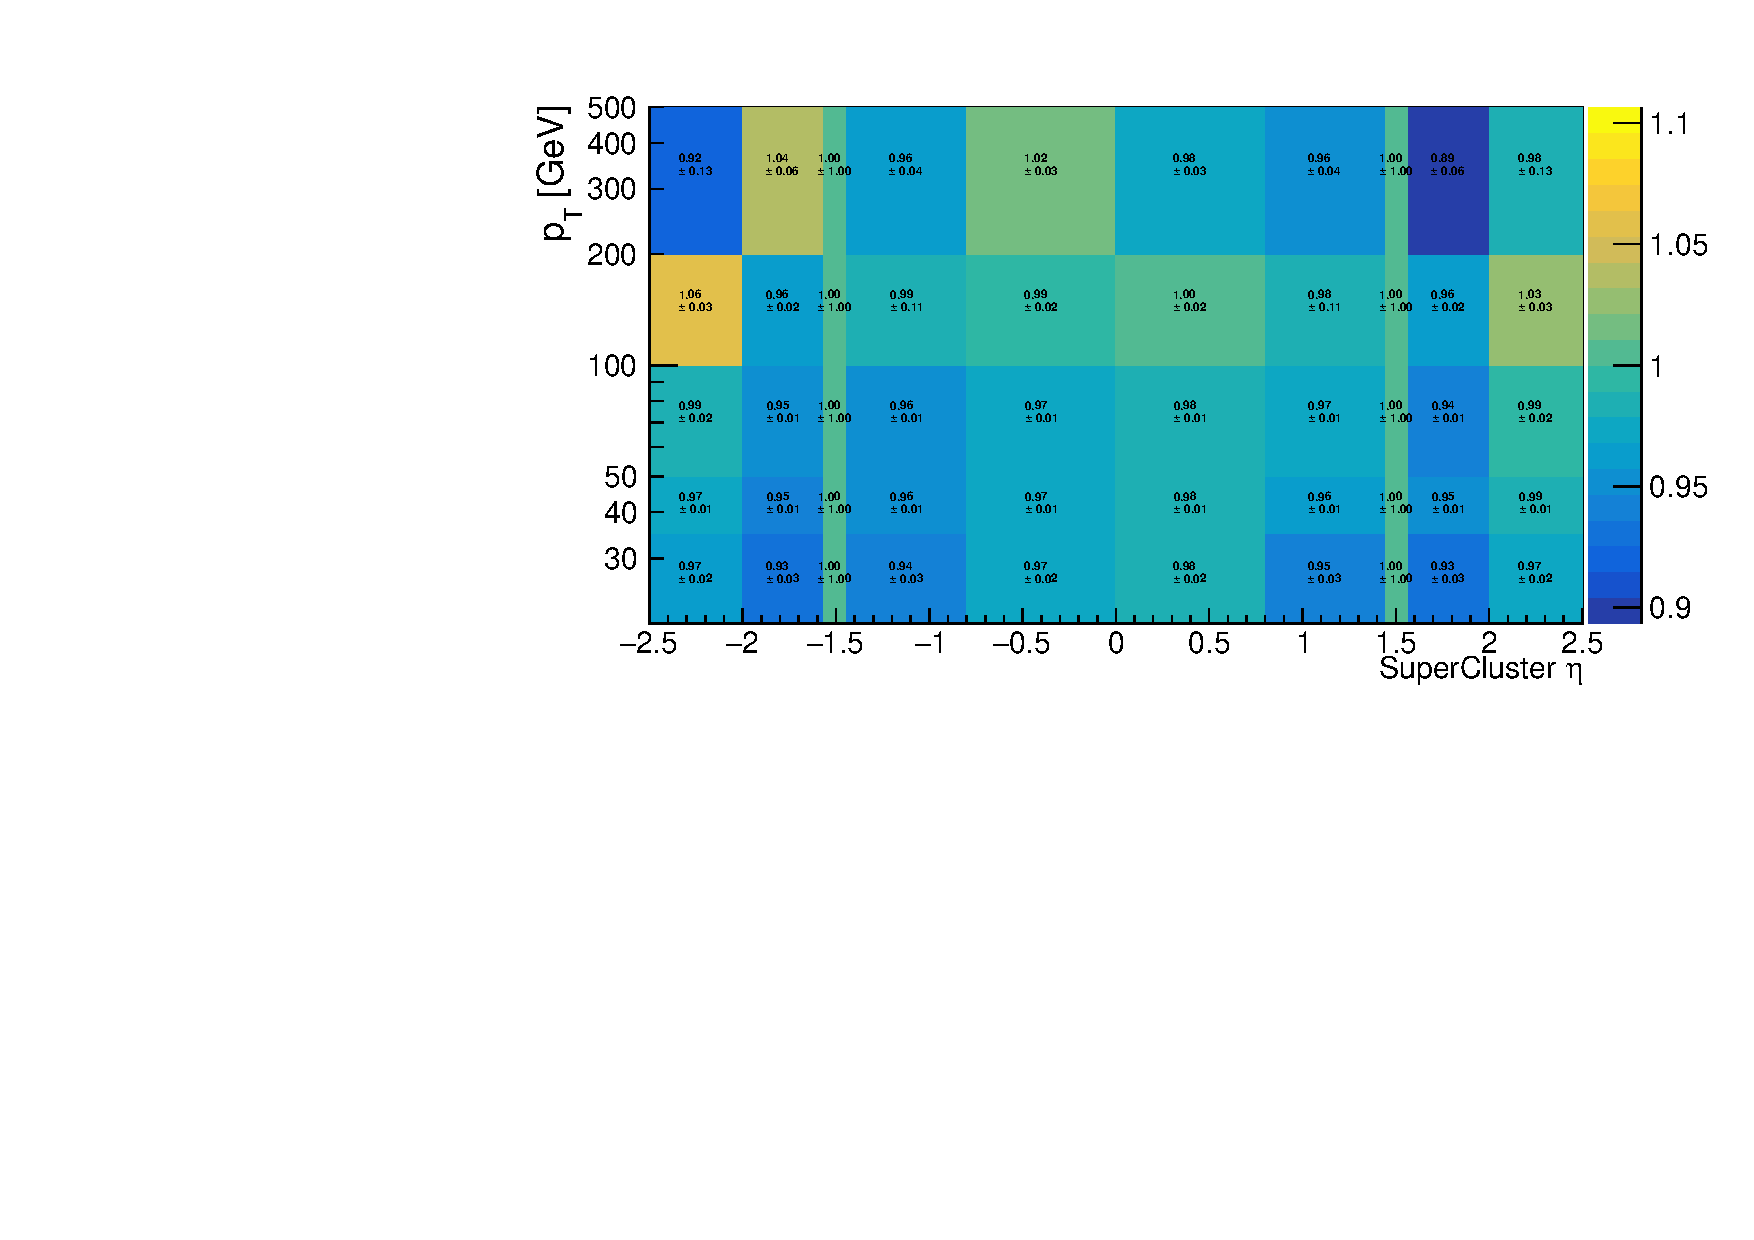
\includegraphics[width=.5\textwidth]{SF/2016_PhotonsMVAwp80_SF2D.pdf}}%
\subfigure [2017]        {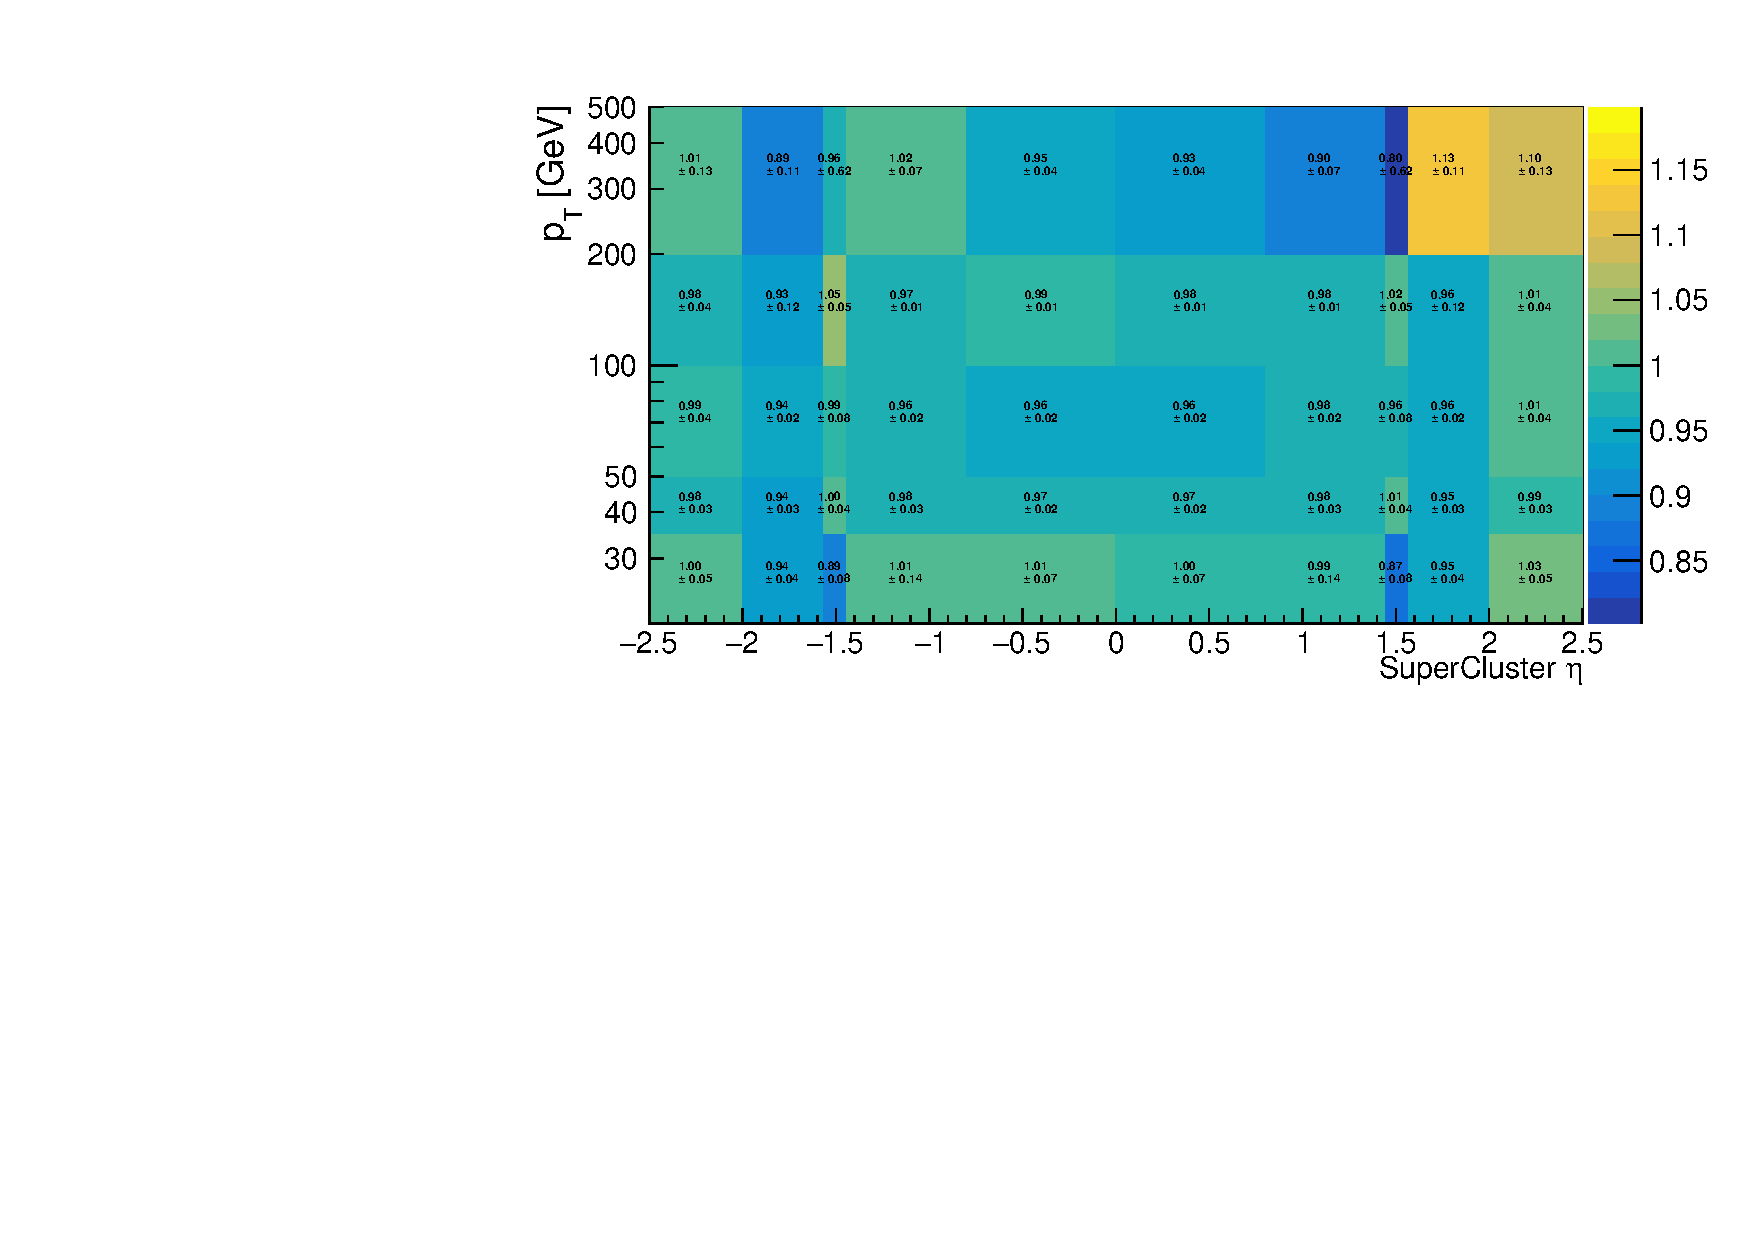
\includegraphics[width=.5\textwidth]{SF/2017_PhotonsMVAwp80_SF2D.pdf}}\\
\subfigure [2018]        {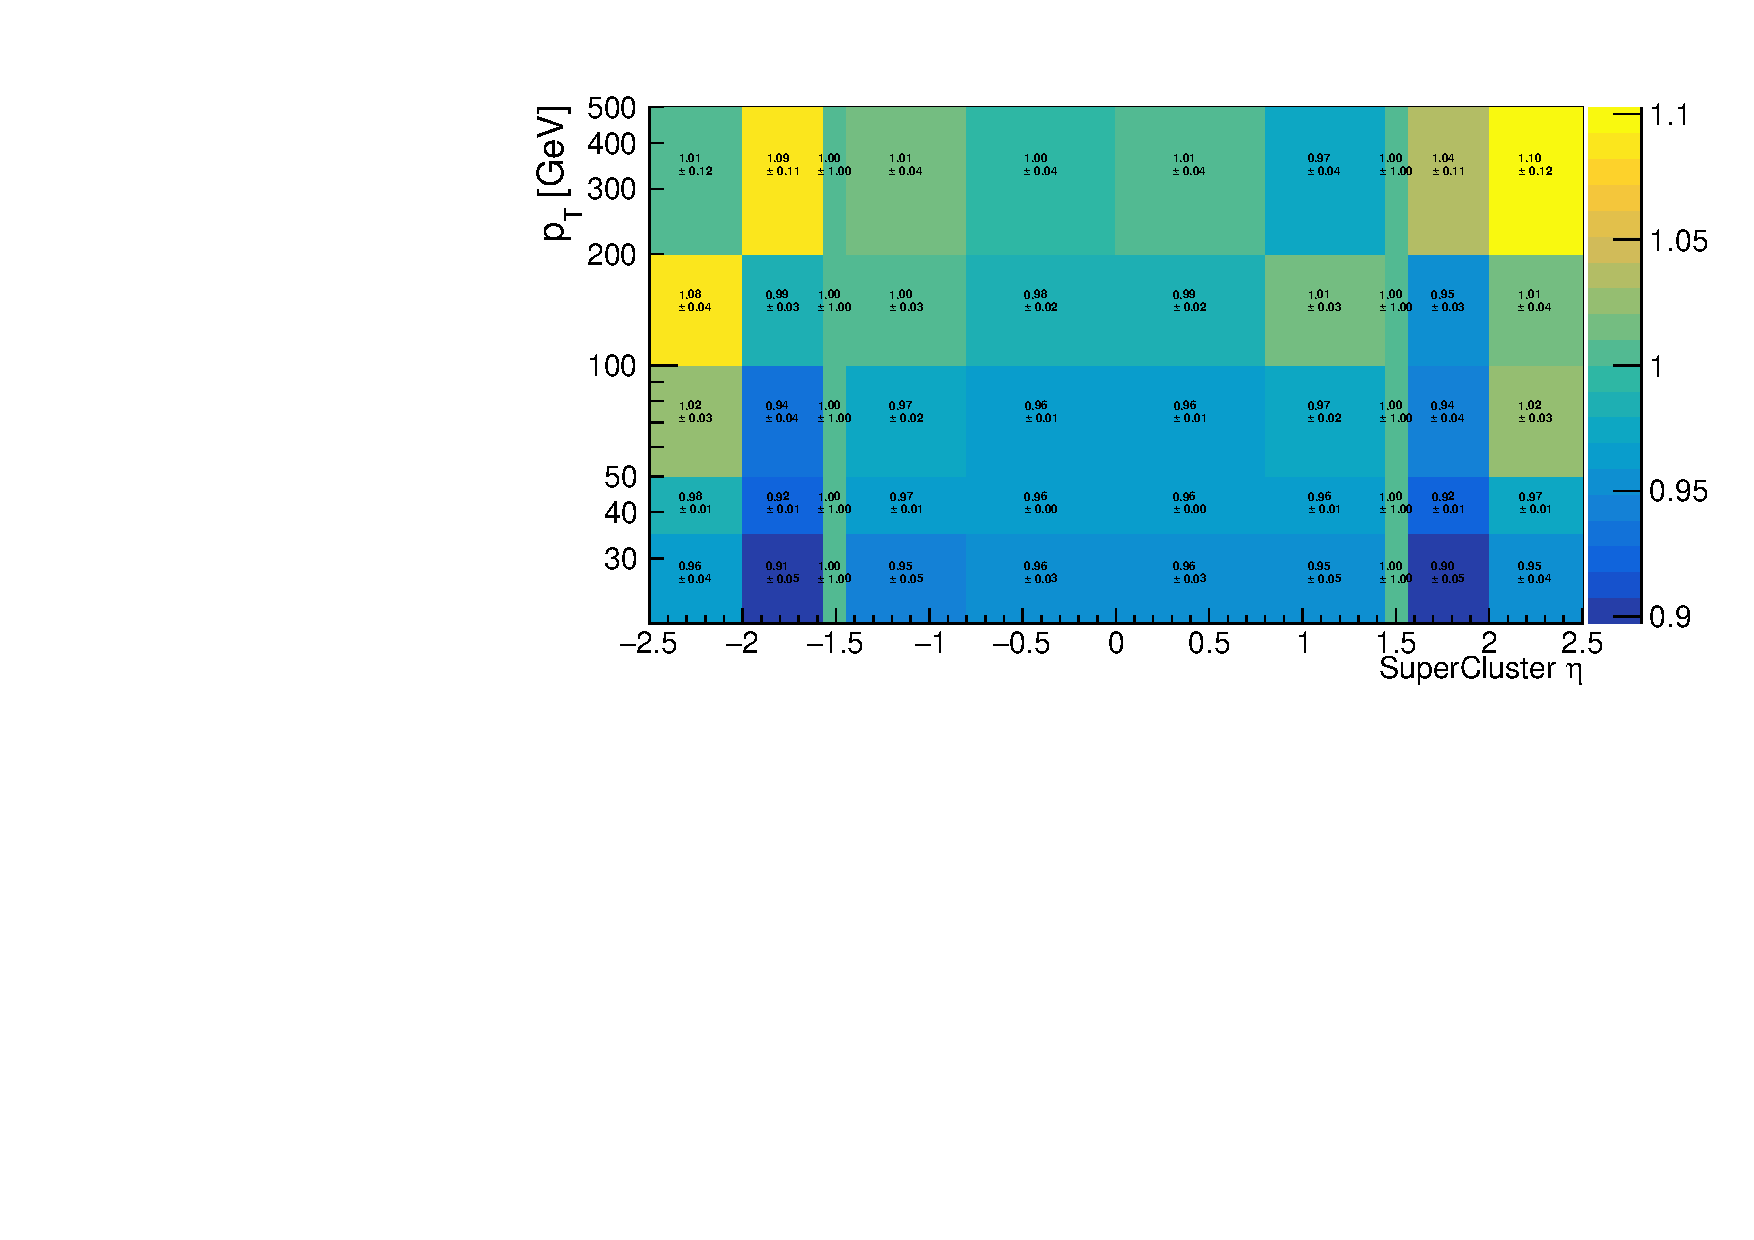
\includegraphics[width=.5\textwidth]{SF/2018_PhotonsMVAwp80_SF2D.pdf}}
\caption{Photon efficiency scale factors for the MVA-based ID with working point \texttt{wp80}.}
\label{fig:phEffMVASF_wp80}
%% }
\end{figure}

\begin{figure}
\centering
\subfigure [2016preVFP ] {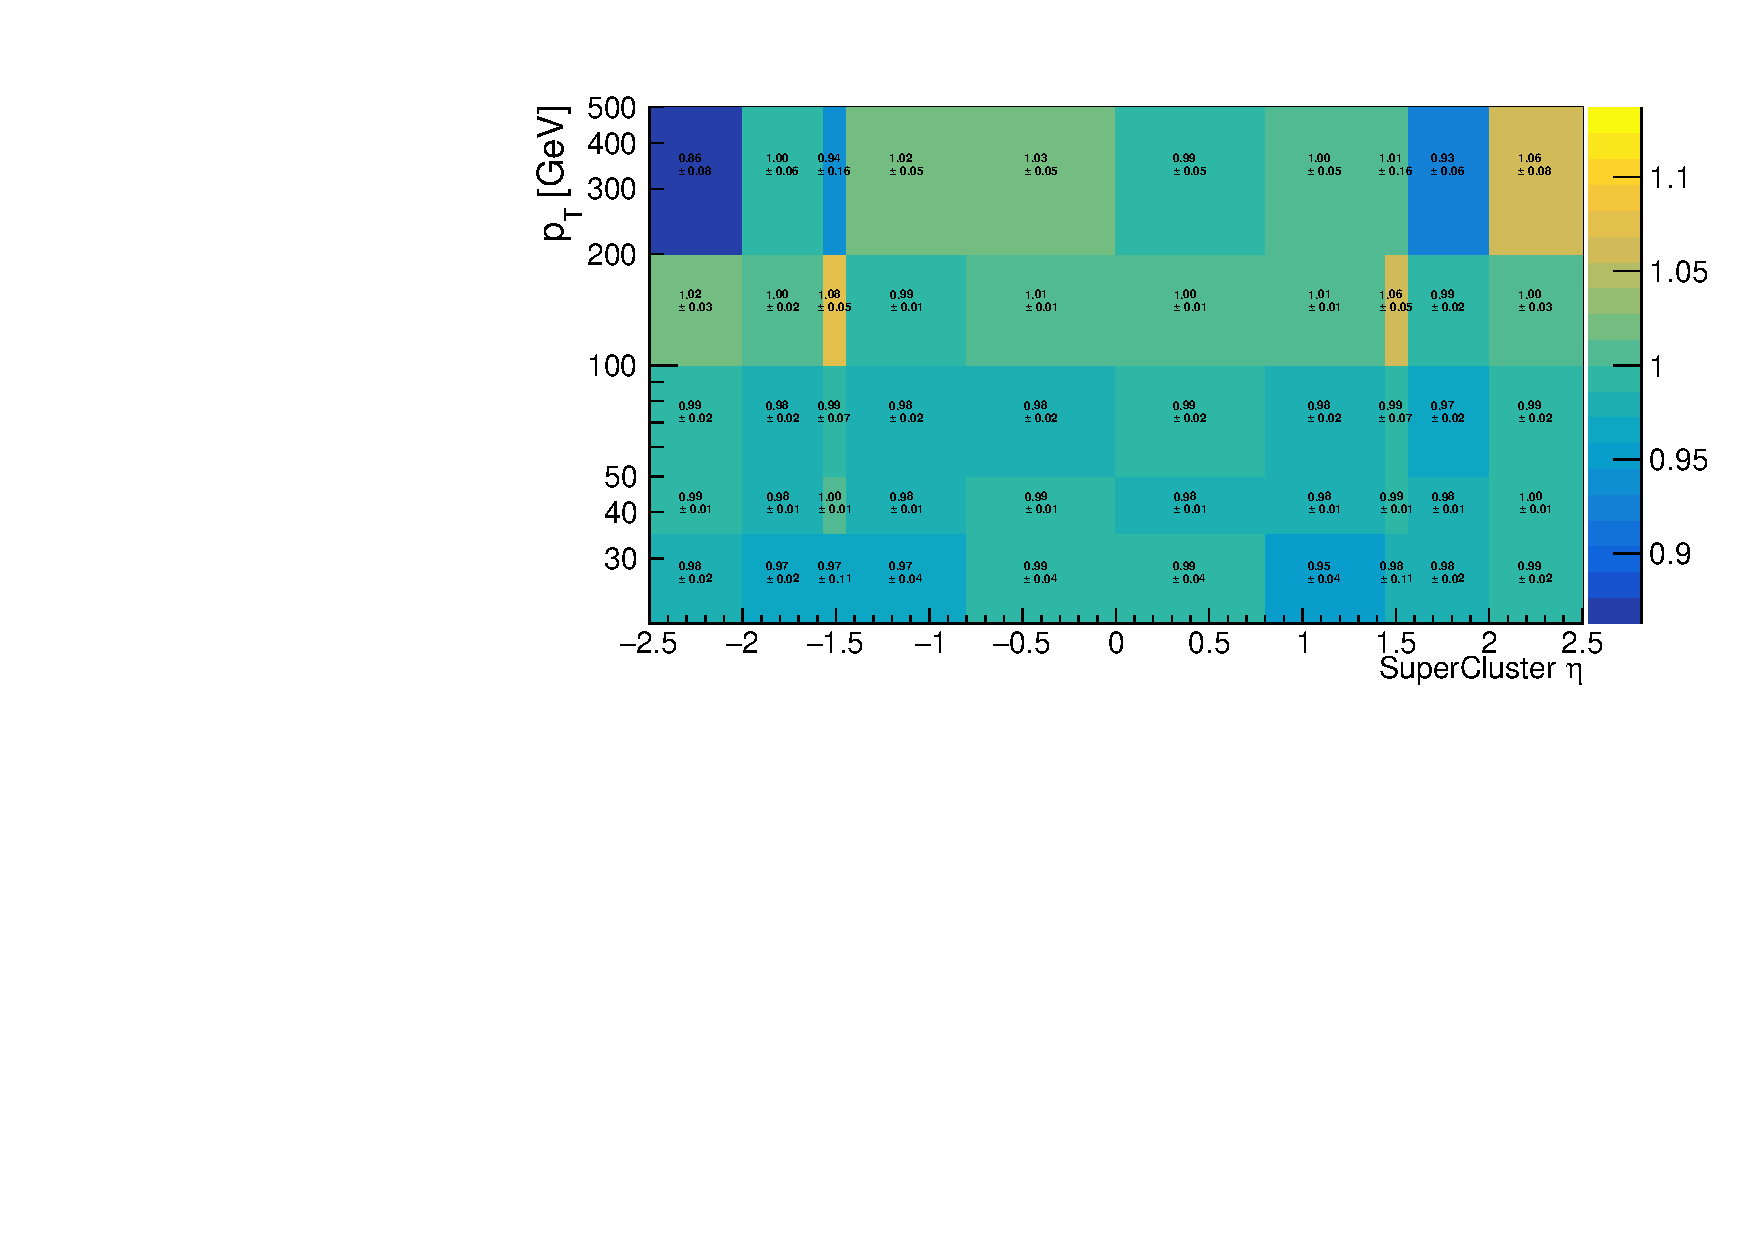
\includegraphics[width=.5\textwidth]{SF/2016_PhotonsMVAwp90_SF2D.pdf}}%
\subfigure [2017]        {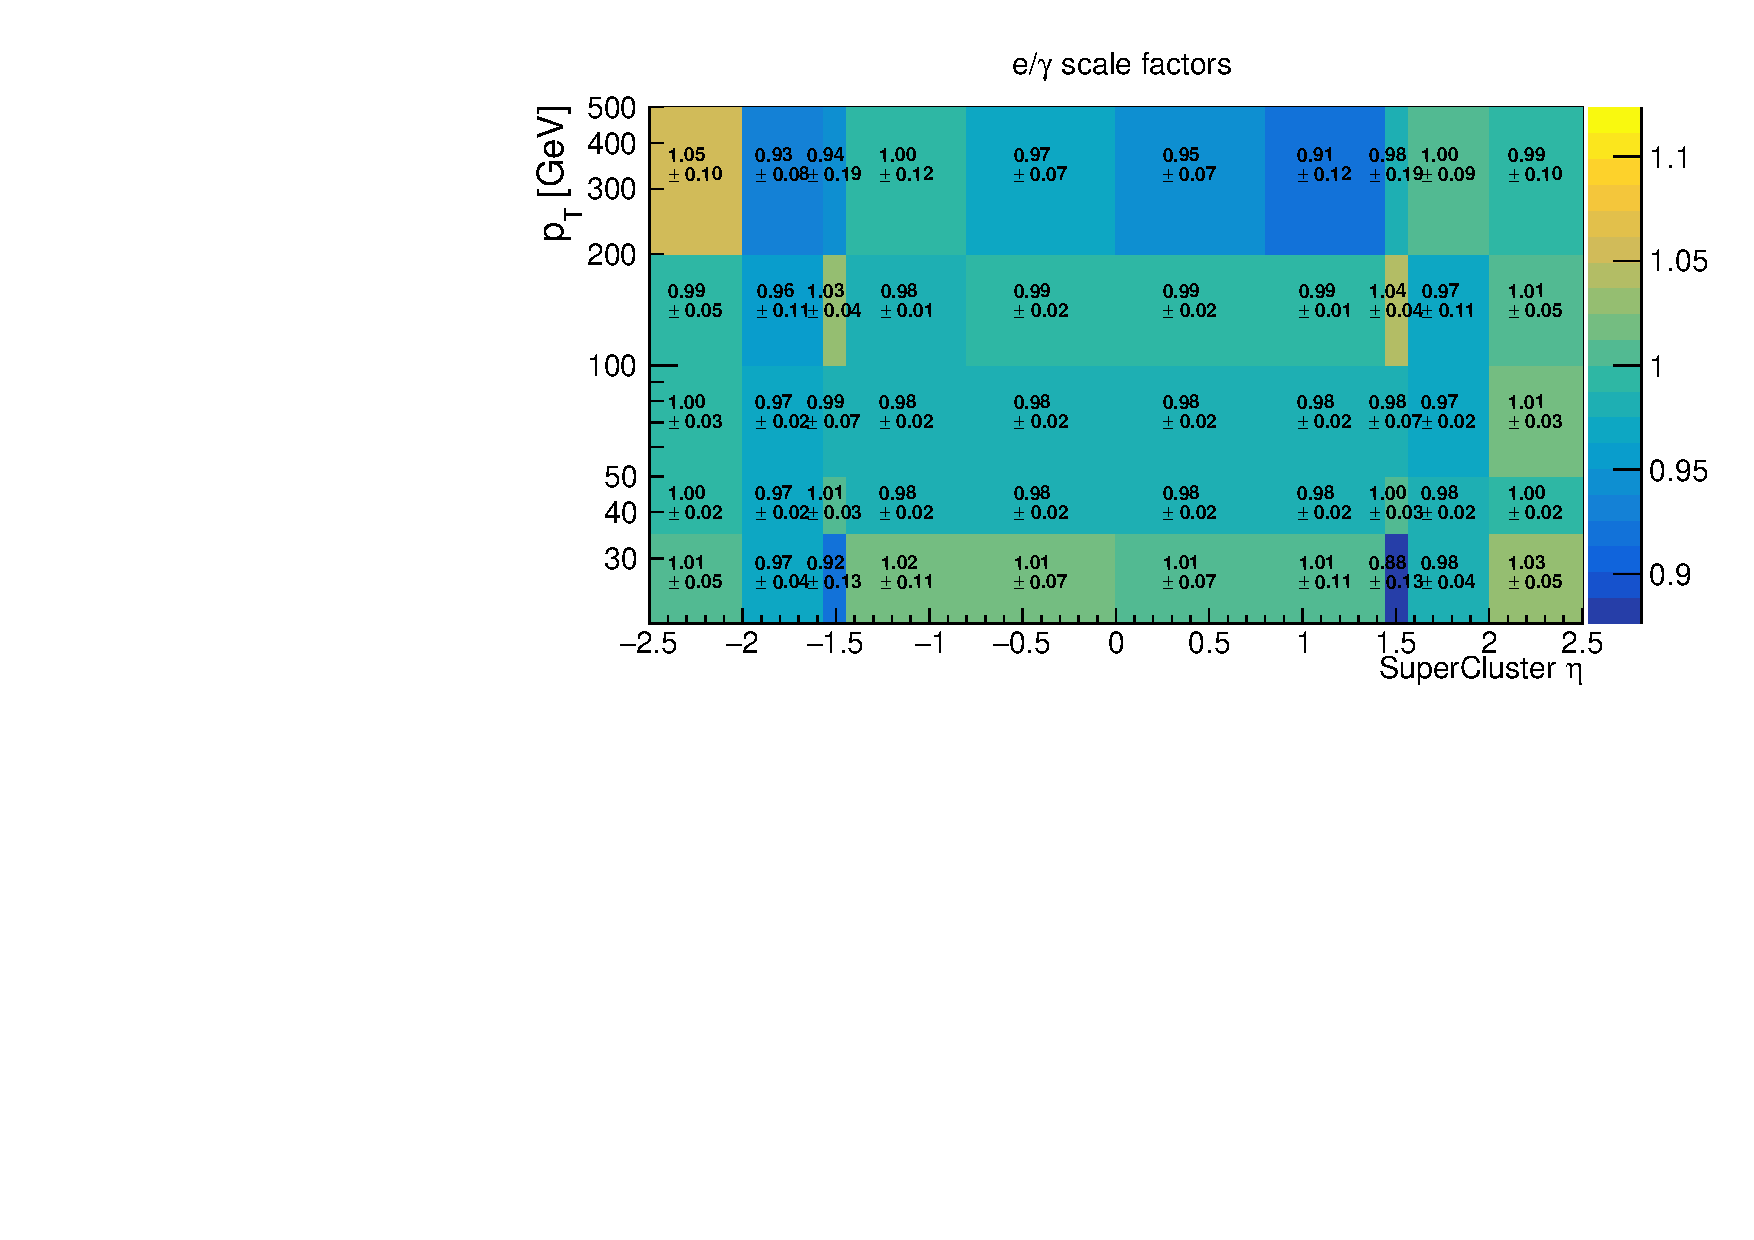
\includegraphics[width=.5\textwidth]{SF/2017_PhotonsMVAwp90_SF2D.pdf}}\\
\subfigure [2018]        {\includegraphics[width=.5\textwidth]{SF/2018_PhotonsMVAwp90_SF2D.pdf}}
\caption{Photon efficiency scale factors for the MVA-based ID with working point \texttt{wp90}.}
\label{fig:phEffMVASF_wp90}
\end{figure}

A comparison between the cut-based and the MVA-based IDs is shown in Figure~\ref{fig:PhotonIsoAUC}.
It represent the background rejection as a function of the signal efficiency for the raw MVA discriminant
and the three working points of the cut-based ID.

\begin{figure}
\centering
\includegraphics[width=.5\textwidth]{PhotonIsoAUC.png}
\caption{Performance of the photon BDT and cut-based identification algorithms in 2017.
Three different working points (loose, medium and tight) are shown for the cut-based ID. \cite{CMS:photon-performance-2015}}
\label{fig:PhotonIsoAUC}
\end{figure}

\paragraph{Selections used in the analysis\\}
\label{sec:photon_selection}

A common base selection is applied to all the photons, consisting of
\pt > 20 \GeV and
$|\eta| < 1.4442$ OR $1.566 < |\eta| < 2.4$.
Photons must also pass a conversion safe electron veto (CSEV) \cite{CMS:photon-performance-2015} which requires the absence of charged particle tracks,
with a hit in the innermost layer of the pixel detector not matched to a reconstructed conversion vertex, pointing to the photon cluster in the ECAL.
Photons are also rejected in the presence of a seed in the pixel tracker consisting of at least two hits,
which points to the ECAL within some window defined around the photon SC position.
Photons that pass these selections are called \textbf{kinematic photons}, which is the loosest selection used in this analysis.

Photons that also pass the cut thresholds of the Loose cut-based ID (see Table~\ref{tab:VPhotonID}) for H/E, the neutral ($I_n$) and photon ($I_\PGg$) isolations
are defined \textbf{very loose} photons.
They are used as the loose working point in a tight-to-loose method (Section \ref{sec:fake_photons_background}) to estimate the \nonprompt photon background.

The photons that also pass the \sieie and charged isolation ($I_{ch}$), and thus the Loose cut-based ID, are the \textbf{loose photons},
which is the tight selection for the \nonprompt photon background,
and the analysis selection for the results derived using the cut-based ID.

Additionally, kinematic photons that pass the MVA-based working points wp90 and wp80 are also considered,
given the improved performance of the MVA ID over the cut-based one.
The drawback of this ID is that it is not possible to do a data-driven estimation of the \nonprompt background,
due to the limited size of the application region defined by requiring a photon that passes the wp90 but fails the wp80,
as explained in Section~\ref{sec:fake_photons_background}.


\subsection{Jets}
\subsubsection{Jet Identification}
\label{sec:jet_ID}
In order to assure a good reconstruction efficiency, identification quality criteria are imposed on jets based on
the energy fraction of the charged, electromagnetic, and neutral hadronic components \cite{CMS-PAS-JME-16-003}.

To reduce instrumental background, the jet identification criteria described in Table \ref{tab:JetID2018} is used.

\begin{table}
  \caption{Jet identification criteria used in \RunII{} with thresholds used for 2018 data.}
  \label{tab:JetID2018}
  \resizebox{\textwidth}{!}{
  \begin{tabular}{l c c c c}
    \toprule
    Variable                    & $|\eta| \le 2.6$ & $2.6 < |\eta| \le 2.7$ & $2.7 < |\eta| \le 3.0$ & $3.0 < |\eta| \le 5.0$\\
    \midrule
    Neutral Hadron Fraction     & < 0.90           & < 0.90                 & -                      & > 0.2                 \\
    Neutral EM Fraction         & < 0.90           & < 0.99                 & $<0.99\ \land\,>0.02$  & < 0.9                 \\
    Number of Constituents      & > 1              & -                      & -                      & -                     \\
    Muon Fraction               & < 0.80           & < 0.80                 & -                      & -                     \\
    Charged Hadron Fraction     & > 0              & -                      & -                      & -                     \\
    Charged Multiplicity        & > 0              & > 0                    & -                      & -                     \\
    Charged EM Fraction         & < 0.80           & < 0.80                 & -                      & -                     \\
    Number of Neutral Particles & -                & -                      & > 2                    & > 10                  \\
    \bottomrule
  \end{tabular}
  }
\end{table}

In this analysis, the jets are required to be within $|\eta| < 4.7$ and to have a transverse momentum above 30\GeV.

The identification of jets originated by the hadronization of heavy-flavour quarks is achieved through the DeepFlavour tagger \cite{Guest_2016, CMS-BTV-16-002}.
It uses a deep neural network with input variables from up to six tracks from each jet, information on secondary vertices and on the jet itself,
such as the energy and total number of tracks.
It assigns five probabilities to each jet, namely to contain only one \PQb hadron, two or more \PQb hadrons, exactly one \PQc hadron, at least two \PQc and no \PQb hadrons, or none of the above.
In the two and three lepton channels there is the need to exclude events containing top quarks,
since their decay $\PQt \to [\PW \to \Pl\PGn] \PQb$ produces additional charged leptons which may lower the purity of the signal regions.
Thus the need to identify jets induced by the hadronization of \PQb quarks,
which is achieved by summing the probabilities of the first two categories,
which are the single b hadron and the two or more b hadrons.
Working points are defined for this ID, as shown in Table \ref{tab:DeepFlavourBtagWP}.

\begin{table}
  \caption{Working points of the combined b-tag with the DeepFlavour classifier and the corresponding misidentification probability.}
  \label{tab:DeepFlavourBtagWP}
  \centering
  \begin{tabular}{l c c}
    \toprule
    \makecell{Working\\point} & Threshold & \makecell{Misidentification\\probability}\\
    \midrule
    Loose  & 0.0494 & 10  \%\\
    Medium & 0.2770 & 1   \%\\
    Tight  & 0.7264 & 0.1 \%\\
    \bottomrule
  \end{tabular}
\end{table}

In addition this analysis considers also a collection of \textbf{large radius jets} clustered using the same \antikt algorithm with a distance parameter $R = 0.8$.
These jets are cleaned using the Pileup Per Particle Identification (PUPPI) \cite{Bertolini_2014}, which is a method for \pileup{} mitigation.

\paragraph{Jet disambiguation\\}
The PF jet collection contains jets clustered with \antikt on all the particles reconstructed from Particle Flow.
This means that isolated and energetic leptons and photons, which are part of the signal definition,
are likely to be in the core of a jet due to the nature of the algorithm.
Therefore a disambiguation strategy is needed to avoid double counting entities.
Jets are removed if they match any of the leptons passing the Loose ID
and photons, either FSR associated to a lepton or candidates passing the kinematic selection (Section \ref{sec:photonID}),
by requiring: $\DR(\text{jet,\,lepton/photon}) > 0.4$.


\subsection{Summary}
The requirements on all objects used for the analysis with 2016, 2017 or 2018 data are summarized in the Table~\ref{tab:objsummary}. In addition, a ``ghost-cleaning'' procedure is applied to the muons, as described in Sec.~\ref{sec:muonReco}. 

A lepton is declared {\bf loose} if it passes the reconstruction, kinematics and dxy/dz cuts and declared {\bf tight} if it passes in addition the identification, isolation and SIP3D requirements. 

\begin{table}
  \centering
  \caption{Summary of physics object selection for the analysis.}
  \label{tab:objsummary}
  %% \resizebox{\textwidth}{!}{
    \begin{tabular}{l l}
      \toprule
      \multirow{4}{*}{Electrons}
        & $\pt^e > 7 \GeV$   \quad $\abs{\eta^e} < 2.5$ \\
        & $d_{xy} < 0.5 \cm$ \quad $d_{z} < 1 \cm$      \\
        & $\SIPthreeD < 4$                              \\
        & MVA ID with isolation cuts from Section~\ref{sec:eleMVA}\\
      \midrule
      \multirow{5}{*}{Muons}
        & Global or Tracker Muon                                 \\
        %% & Discard muons with muonBestTrackType==2 even if they are global or tracker muons \\
        & $\pt^{\mu} > 5 \GeV$ \quad $\abs{\eta^{\mu}} < 2.4$    \\
        & $d_{xy} < 0.5 \cm$   \quad $d_{z} < 1 \cm$             \\
        & $\SIPthreeD < 4$                                       \\
        & BDT with ID, isolation from Section~\ref{sec:muo_selection}\\
      \midrule
      \multirow{4}{*}{FSR photons}
        & $\pt^{\PGg} > 2 \GeV$ \quad $\abs{\eta^{\PGg}} < 2.4$     \\
        & ${\cal I}_{\mathrm{PF}}^{\PGg} < 1.8$                     \\
        & $\DR(\ell,\,\PGg) < 0.5$                                  \\
        & $\frac{\DR(\Pl,\,\PGg)}{(\pt^{\PGg})^2} < 0.012 \GeV^{-2}$\\
        \noalign{\vspace{.3ex}} % small vertical space
      \midrule
      \multirow{5}{*}{Signal photons}
        & $\pt^{\PGg} > 20 \GeV$                        \\
        & $\abs{\eta^{\PGg}} < 2.4 \; \land \abs{\eta^{\PGg}} \notin (1.4442, 1.566) $\\
        & $\DR(\ell,\,\PGg) > 0.5$                      \\
        & Conversion Safe Electron Veto                 \\
        & Cut-based (Loose wp) or MVA (wp90 or wp80) ID \\
      \midrule
      \multirow{5}{*}{Jets}
        & $\pt^{\mathrm{jet}} > 30 \GeV$ \quad $\abs{\eta^{\mathrm{jet}}} < 4.7$ \\
        & $\DR(\ell/\PGg,\, \mathrm{jet}) > 0.4$    \\
        & Cut-based jet ID (tight WP)               \\
        & Jet \pileup{} ID (tight WP)               \\
        & Deep CSV b-tagging (medium WP)            \\
      \bottomrule
    \end{tabular}
  %% }
\end{table}


\section{Calibration and efficiency measurements}
Electron and Muon identification criteria, energy/momentum calibrations, and efficiency measurements,
as well as the Final State Radiation (FSR) recovery, follow the same strategy used in Reference \cite{CMS-SMP-20-001}. % and CMS_AN_2016-442 CMS_AN_2017-342

\subsection{Electrons}
\subsubsection{Electron Energy Calibrations}
%\textbf{FIXME: ReRecoed data are used but additional e-scale and smearing corrections NOT yet available and thus NOT yet applied}
Electrons in data are corrected for features in ECAL energy scale
in bins of $\pt$ and $\left| \eta \right|$. Corrections are calculated
on a $\cPZ \to \Pe\Pe$ sample to align the dielectron   
mass spectrum in the data to that in the MC, and to
minimize its width.

The $\cPZ \to \Pe\Pe$ mass resolution in Monte Carlo is made to match
data by applying a pseudo-random Gaussian smearing to electron energies,
with Gaussian parameters varying in bins of $\pt$ and $\left| \eta \right|$.
This has the effect of convoluting the electron energy spectrum with a
Gaussian.

The electron energy scale is measured in data by fitting a Crystal-ball function to the di-electron mass spectrum around the Z peak in the $Z\rightarrow \Pe \Pe$ control region.
% The energy scale for the 2016, 2017 and 2018 dataset are shown in Fig.~\ref{fig:ele_energy_scaleA},~\ref{fig:ele_energy_scaleB},~\ref{fig:ele_energy_scaleC} (a), respectively, and decently agrees with the MC with the preliminary corrections released so far by EGAMMA POG. % for Moriond. % even without any corrections available at the moment. 


\subsubsection{Electron Efficiency Measurements}
\label{sec:eleEffMeas}
Electron efficiencies are evaluated using the Tag-and-Probe method~\cite{CMS-EWK-10-005}.
The study was performed on the SingleElectron/EGamma dataset for each year separately.

Tag electrons need to satisfy the following quality requirements:
\begin{itemize}
\item trigger matched to single electron trigger;
\item $\pt > 30 \GeV$, supercluster (SC) $|\eta| < 2.17$;% but on in EB-EE gap ($1.4442<|\eta|<1.566$)
\item the tag and the probe need to have opposite charge.
%\item tight working point of the Spring16 cut-based electron ID
\end{itemize}

For the bin of probe \pt between 7 and 20\GeV, additional criteria are required:
\begin{itemize}
\item the tag has to pass a cut on the MVA score;
\item $\sqrt{2*\ptmiss*\pt^{tag}*(1-cos(\phi_{\rm MET}-\phi_{tag}))} < 45 \GeV$;
\item tag minimum \pt increased to 50\GeV;
\item the charge is determined with the so-called selection method, requiring that all three estimates of the electron charge to agree.
\end{itemize}
These cuts help cleaning the background and make the fits more reliable (and thus, the measurement more precise).

Probe electrons only need to be reconstructed with the Gaussian sum filter, while the FSR recovery algorithm is not applied.

The nominal simulation efficiencies are evaluated from the a Drell-Yan sample simulated with \MADGRAPH at Leading Order in QCD,
using a template fit.
The $m_{ee}$ signal shape of the passing and failing probes are taken from MC and convoluted with a Gaussian.
The data is then fitted with the convoluted MC templates and a CMSShape (an Error-function with a one-sided exponential tail).
For the low \pt bins, a Gaussian is added to the signal model for the failing probes.

%\paragraph{Electron selection efficiency measurements}\mbox{}\\
%\label{par:Efficiency_measurements}

The electron selection efficiency is measured as a function of the probe electron $p_{T}$ and its SC $\eta$, and separately for electrons falling in the ECAL gaps.

%Figure \ref{fig:ele_sel_pt_turn_onA},~\ref{fig:ele_sel_pt_turn_onB},~\ref{fig:ele_sel_pt_turn_onC} and~\ref{fig:ele_ele_eta_turn_onA},\ref{fig:ele_ele_eta_turn_onB},~\ref{fig:ele_ele_eta_turn_onC} show the $p_{T}$ and $\eta$ turn-on curves measured in data, for 2016, 2017 and 2018.
% and the final 2D scale factor is shown in Fig.~\ref{fig:ele_sel_scale_factors} together with the systematic uncertainties. %These scale factors are very similar to the ICHEP figures, but more homogenous across $\eta$ and $p_{T}$ because of the higher statistics and the usage of more stable fitting routines in the new T\&P tool.

%\includegraphics[page=2, width=0.4\textwidth]{Figures/Electrons/ErecoEta}\\

Standard practices for the evaluation of Tag-and-Probe uncertainties for efficiency measurements are followed. Specifically, the following were considered:

\begin{itemize}
   \item Variation of the signal shape from the MC shape to an analytic shape (Crystal Ball) fitted to the MC
   \item Variation of the background shape from a CMS-shape to a simple exponential in fits to data
   \item Using an NLO MC sample for the signal templates
\end{itemize}

The total uncertainty for the measurement of the scale factors is the quadratic sum of the statistical uncertainties returned from the fit and the aforementioned systematic uncertainties.

The resulting efficiencies and corresponding scale factors, expressed as ratio of the efficiency observed in data to that calculated in simulation are reported
in Figure~\ref{fig:eleMVAEffSF}.

\begin{figure}
\centering
\includegraphics[width=.5\textwidth]{eleMVAEffSF2017.png}
\caption{Electron selection efficiencies in data (upper panel)
  and data-to-simulation ratio (lower panel),
  measured using the Tag-and-Probe technique
  as a function of the transverse energy}
\label{fig:eleMVAEffSF}
\end{figure}



\subsection{Muons}
\subsubsection{Muon Energy Calibrations}
Similar to electrons the muon momentum scale is measured in data by fitting a Crystal-ball function to the di-muon mass spectrum around the Z peak in the 
$Z \rightarrow \mu\mu$ control region.
%At the moment no muon scale and resolution corrections are available but from 
%Fig.~\ref{fig:mu_energy_scaleA},~\ref{fig:mu_energy_scaleB} and~\ref{fig:mu_energy_scaleC} shows a very good agreement between data and simulation, for 2016, 2017 and 2018 eras, respectively. %even without any corrections.



\subsubsection{Muon Efficiency Measurements}
\label{sec:muonEffMeas}
Muon efficiencies are measured with the Tag and Probe (T\&P) method performed on
$\cPZ \to \Pgm\Pgm$ and $\JPsi\to\mu\mu$ events in bins of $\pt$ and $\eta$. 
% More
%details on the methodology can be found in Ref.~\cite{CMS_AN_2015-277}. Measurements are extracted using 2018 RunA,B,C,D data while the measurements corresponding to 2016 and 2017 datasets have already been reported in Ref.~\cite{CMS_AN_2016-442} and Ref.~\cite{CMS_AN_2017-342} respectively.
%
The $\Z$ sample is used to measure the muon reconstruction and identification efficiency at high $\pt$,
and the efficiency of the isolation and impact parameter requirements at all $\pt$.
%
The $\JPsi$ sample is used to measure the reconstruction efficiency at low $\pt$,
as it benefits from a better purity in that kinematic regime. In this case,
events are collected using \verb=HLT_Mu7p5_Track2_Jpsi_v*= when probing the
reconstruction and identification efficiency in the muon system, and using the
 \verb=HLT_Mu7p5_L2Mu2_Jpsi_v*= when probing the tracking efficiency.

Results for the muon reconstruction and identification efficiency for $\pt > 20\GeV$
have been derived by the Muon POG.
The probe in this measurement are tracks reconstructed in the inner tracker, and
the passing probes are those that are also reconstructed as a global or tracker muon 
and passing the Muon POG Loose muon identification.
%
Results for low \pt muons were derived using \JPsi events, with the same definitions
of probe and passing probes. The systematic uncertainties are estimated by varying the analytical signal and background shape models used to fit 
the dimuon invariant mass. 
% Details on the procedure can be found in Ref.~\cite{AN-15-277}. 
The efficiency and scale 
factors used for low $\pt$ muons are the ones derived using single muon dataset.


For the impact parameter requirements, the measurement is performed using $\Z$ events. Events are selected with \verb=HLT_IsoMu27_v*= or \verb=HLT_Mu50_v*= triggers.
For this measurement, the probe is a muon passing the POG Loose identification criteria,
and it is considered a passing probe if satisfies the SIP3D, dxy, dz cuts of this analysis.
%
The efficiency to reconstruct a muon track in the inner detector is measured using as probes tracks
reconstructed in the muon system alone. The efficiency and 
data to MC scale factors are measured from Z events as a function of $\eta$ for $\pt > 10\GeV$ and $\pt < 10\GeV$. 

%he values of data to mc scale factors 
%used are from the ReReco version of the full dataset collected in 2018. 

%The tracking efficiency in data and simulation as a function of $\eta$ is shown in Fig.~\ref{fig:MuonIDEff_4}.
%\begin{figure}[htbp]
%  \begin{center}
%    \subfigure[]{\includegraphics[width=0.42\textwidth]{Figures/Muons/Placeholder.png}}
%    \subfigure[]{\includegraphics[width=0.42\textwidth]{Figures/Muons/Placeholder.png}}
%    \caption{Tracking efficiency in data and simulation as a function of $\eta$ for muon $\pt < 10\GeV$(left) and $\pt > 10\GeV$(right) with ReReco data.}
%    \label{fig:MuonIDEff_4}
%\end{center}
%\end{figure}


\clearpage


\subsection{Jet Energy Corrections}
The calorimeter response to particles is not linear and it is not straightforward to translate the measured jet energy
to that of the original parton.
In data, these deviations are driven by the non-uniformity and non-linearity of the calorimeter response,
while in Monte Carlo simulation, the corrections ensure a posteriori the agreement with the observed data.
Furthermore, contributions from \pileup{} events or detector noise may bias the measurement of the jet energy.
To this end, a calibration of the reconstructed jet is performed by applying a series of corrections on the measured jet energy,
collectively referred to as Jet Energy Scale corrections (JES).
%% This class of corrections represents an important source of systematic uncertainty in the analyses with a multi-jet final state.

\begin{figure}
\centering
\includegraphics[width=.8\textwidth]{JEC_levels.png}
\caption{Overview of the jet energy calibration procedure followed in data and simulation~\cite{CMS-JME-13-004}.}
\label{fig:JECoverview}
\end{figure}

%% The corrections, parametrized as function of \pt and $\eta$ of the jets, are applied following the standard procedure used by most of the CMS analyses \cite{CMS:JEC_2011, CMS-DP-2016-020, CMS-DP-2021-033}.

\paragraph{Jet energy scale\\}
The JES corrections are calculated in the form of a multiplicative factor on the four-momentum of the measured jet,
in order to match the measured energy of each jet to its true energy at the generator level.
The measured jet transverse momentum response is defined as the ratio of the measured jet \pt at the reconstruction step to the generated jet at particle level.
%% These corrections and the corresponding uncertainties are provided centrally by the CMS JetMet group

\Pileup{} offset corrections account for the measured energy of the jet in excess due to
the presence of in-time (IT) and out-of-time (OOT) \pileup{}
%% They are derived from the simulation of QCD multi-jet events processed with or without \pileup{} overlay
and they are applied to both data and MC samples.

Simulated response corrections compensate for the non-linear response in \pt and pseudorapidity
from the calorimeters and tracker coverage and they are parametrized as a function of these jet kinematic variables.

Residual data to Monte Carlo corrections are applied to improve the agreement as a function of the jet $\eta$ and \pt.
The absolute scale of the measured jet \pt response is corrected in data using multi-jet and Drell-Yan plus jets events,
which benefit from the high precision measurement of the \PZ boson and the photon energy in the ECAL.
The residual $\eta$ correction is derived in di-jet events exploiting the \pt imbalance of the di-jet system.

\paragraph{Jet energy resolution\\}
Jet Energy Resolution (JER) corrections introduce a dose of smearing in the simulated jet \pt spectrum
to compensate for data-to-simulation differences due to detector resolution effects.
They are determined in $\PGg/\PZ$ + jets events by fitting the residual of the \pt distribution to a
double-sided Crystall Ball function.
This accounts for a gaussian core due to statistical fluctuations in the deposited energy,
while the tails account for effects such as inactive areas, neutrino emissions in heavy flavour in-flight decays
or punch-though of hadrons beyond the end of the calorimeter.


\subsubsection{L1 prefiring}
\label{sec:L1Prefiring}
In 2016 and 2017, the gradual timing shift of ECAL was not properly propagated to \Lone trigger primitives (TP)
resulting in a significant fraction of high eta TP being mistakenly associated to the previous bunch crossing~\cite{CMS-TRG-17-001}.
Since \Lone trigger rules forbid two consecutive bunch crossings to fire,
in addition to missing the trigger primitive in the correct bunch crossing,
events can self veto if a significant amount of ECAL energy is found in the region of $2<|\eta|<3$.
This effect is not described by the simulations.

A similar effect is present in the muon system, where the bunch crossing assignment of the muon candidates can be wrong due to the limited time resolution of the muon detectors.
This effect was most pronounced in 2016, but is non-zero for both 2017 and 2018.
The associated prefiring rate is stable for $\pt > 25 \GeV$ but affects the almost entire eta range.
Its magnitude varies between 0\% and a 3\%.

The probability not to prefire (see Equation~\ref{eq:L1prefiring} is calculated for each event and applied as a weight to simulation for 2016 and 2017 samples,
using a software tool developed by CMS \Lone trigger experts.
\begin{equation}
\label{eq:L1prefiring}
w^{pref} = 1 - \Probability(prefire) = \prod_{i\, \in\, \PGg,\, jets,\, \PGm} (1 - \epsilon_i^{pref}(\eta, \pt))
\end{equation}

The Figure~\ref{fig:L1Prefiring} shows the impact of the L1 pre-firing weights on the signal MC.
The uncertainty of the weights is reflected in a shift
on the normalization of the signal sample of around 0.2\usep\%.

\begin{figure}
\subfigure [L1 pre-firing weights]       {\includegraphics[width=.5\textwidth]{Figures/L1Prefiring_ZZGTo4LG.png}}%
\subfigure [Effect on $m_{4\ell\gamma}$] {\includegraphics[width=.5\textwidth]{Figures/SYS/SR4P/ZZGTo4LG_mZZGloose_L1Prefiring.pdf}}
\caption{L1 pre-firing weights and their uncertainty on the signal MC in the signal region with four tight leptons and one photon in 2018.
The photon is required to pass the Loose working point of the cut-based ID.}
\label{fig:L1Prefiring}
\end{figure}


\clearemptydoublepage
\chapter{Analysis Strategy}

The analysis aims at observing triboson production of $\PZ\PZ\PGg$ and $\PW\PZ\PGg$, by combining three orthogonal channels.
The \textit{channels} are defined based on the number of leptons in the event.
The four charged lepton channel (4\Pl) targets the $\PZ\PZ\PGg$ production with fully leptonic decay of the two Z bosons.
The three charged lepton channel (3\Pl) is designed primarily for the $\PW\PZ\PGg$ production, in the fully leptonic decay channel of the \PW and \PZ bosons.
Finally, the two charged lepton channel (2\Pl) targets both the $\PZ\PZ\PGg$ and $\PW\PZ\PGg$ production, where one \PZ decays to leptons,
and the other massive boson decays to quarks, which hadronize to jets.

Each channel is studied using several \textit{regions},
based on the number of leptons that pass the tight selection (Sections \ref{sec:ele_selection} and \ref{sec:muo_selection}),
and whether or not there is a photon that passes the tight selection (Section \ref{sec:photonID}).
%% The full scope of the division is illustrated in Table \ref{tab:region_definition}.

The main results reported in this analysis are for the four lepton channel,
while
%% My contribtion to this analysis includes the architecture of the overall strategy in three orthogonal channels,
%% the \nonprompt photon background estimation technique and its application to this analysis.
%% \todo{This needs rephrasing}

\section{Signal}
\label{sec:signal}
This analysis searches for the simultaneous production of two massive bosons and a photon in a single hard scattering of a proton-proton collision at 13\TeV.
The signature of these processes varies among the three channels, but includes a number of high-momentum, isolated leptons,
with one or two pairs resonating to the Z boson mass,
and an isolated photon with high momentum.

The massive bosons are not stable particles and the most simple process that includes the VV\PGg production is 2 fermions $\to$ 4 fermions + a photon.
All Feynman diagrams with the same perturbative order, the minimal case being $\text{O}(\alpha_{EW}^5)\times\text{O}(\alpha_{QCD}^0)$,
must be taken into account in the generation of the signal process,
resulting in a certain degree of ambiguity in what can be considered triboson production when a photon is present in the final state.
We can classify the diagrams into three classes:

\begin{enumerate}
\item The photon is radiated from an initial state fermion (Figure~\ref{fig:ppTo4LG_hard}), a case that includes Initial State Radiation (ISR) diagrams.
\item The photon emerges from a Triple or Quartic Gauge Coupling (e.g. Figure~\ref{fig:ppTo4LG_GC}).
\item The photon is emitted as Final State Radiation (FSR) by one of the leptons from the decay of a vector boson (e.g. Figure~\ref{fig:ppTo4LG_FSR}).
\end{enumerate}
Arguably, only the first and second process are strictly considerable triboson production.

The goal of this analysis is to measure both the cross sections and the significance of the inclusive processes
$pp \to 4\Pl \PGg$, $pp \to 3\Pl \PGnl \PGg$ and $pp \to 2\Pl 2j \PGg$
and of triboson production
in a region where diagrams of che classes 1 and 2 are enhanced.
Therefore a dedicated cut %% , described in Section \ref{sec:FSR_cut},
was devised to suppress events in which the (genuine) photon comes from final state radiation,
and results are derived both with (\textbf{triboson fiducial region}) and without (\textbf{inclusive cross section region}) applying it.

It is worth noting that in the SM only $\PW\PZ\PGg$ can be produced via triple and quartic gauge couplings,
while $\PZ\PZ\PGg$ does not have any leading order (perturbative expansion up to $\alpha_{EW}^5$) contribution from TGC nor QGC.

\begin{figure}
  \centering
  \subfigure [From an initial-state fermion] {\includegraphics[width=.319\textwidth]{triboson_4LG.pdf} \label{fig:ppTo4LG_hard}}
  \subfigure [From non-abelian coupling]     {\includegraphics[width=.319\textwidth]{QGC_3LNuG.pdf}    \label{fig:ppTo4LG_GC}  }
  \subfigure [From a final-state fermion]    {\includegraphics[width=.319\textwidth]{ZZ_4LG.pdf}       \label{fig:ppTo4LG_FSR} }
\caption{Representative Standard Model Feynman diagrams that yield four isolated leptons and a photon in the final state.}
\label{fig:ppTo4LG}
\end{figure}

\paragraph{Signal components\\}
The relative composition of the diagrams shown in Figure~\ref{fig:ppTo4LG} in the signal sample was assessed in a generator level study.
The study is conducted on the four lepton channel, but the results can be generalised to the other two.
Two samples were generated at Leading Order EW ($\alpha_{\rm EW}^5 \, \alpS^0$) using \MADGRAPH.
The first is the inclusive production of four fermions and a photon, while the other constrains the intermediate vector boson state.

More precisely, the first sample simulates the process $\Pp\Pp \to 2\Pe 2\PGm \PGg$,
which in \MADGRAPH syntax corresponds to \verb|generate p p > e+ e- mu+ mu- a|.
The photon may be attached either to an initial- or final-state fermion line,
but not to a triple or quartic vertex since there are no suitable couplings in the SM for this final state.
The choice of a final state where the two lepton pairs have different flavour
excludes the interference from diagrams with the momenta of two leptons swapped.
The computed cross section is $0.075 \fbinv$.

The second sample forces the intermediate Z boson resonances $\Pp\Pp \to \PZ\PZ\PGg \to 2\Pe 2\PGm \PGg$,
using the syntax:
\begin{verbatim}
define ze = z
define zmu = z
generate p p > ze zmu a, ze > e+ e-, zmu > mu+ mu-
\end{verbatim}
In this case the photon is forced to be directly attached to an initial-state fermion line,
making this a sub-sample of the previous one.
The computed cross section is $0.027 \fbinv$.

The distributions of the invariant mass of the same-flavour opposite-sign lepton pairs and the transverse momentum of the photon
for the first and second sample are shown in Figure~\ref{fig:genstudy}.
From these plots it appears that in a sizeable fraction of FSR events the mass of one of the
reconstructed $\Pl\Pl$ pairs is significantly lower than the \PZ peak.
It is also visible that the transverse momentum of FSR photons tends to be lower,
since the momentum of the lepton may change significantly,
and it becomes almost zero above $80\GeVc$.
However only a fraction of the events in both samples are in the tail with $\pt^\PGg > 80\GeVc$.

\begin{figure}
  \centering\hfill
  \subfigure [$m_{\Pl\Pl}$] {\includegraphics[width=.45\textwidth]{genstudy_mll.pdf}}\hfill
  \subfigure [$\pt^\PGg$]   {\includegraphics[width=.45\textwidth]{genstudy_ptGamma.pdf}}\hfill\mbox{}
  \caption{Invariant mass of the same-flavour opposite-sign lepton pairs and the transverse momentum of the photon
  in the two MC samples produced for the study of the fraction of FSR events in the $\Pp\Pp \to 4\Pl\PGg$ process.}
  \label{fig:genstudy}
\end{figure}


\subsection{Signal definition}
\label{sec:signal_definition}
% the signal definition at gen level
The fiducial phase space definition mimics the selection applied to reconstructed events, described in Section \ref{sec:event_selection}.

The charged leptons, either electrons or muons are required to have $\pt > 5 \GeV$ and $|\eta| < 2.5$.
Each lepton pair $\Pl_i, \Pl_j$ must be separated $\DR(\Pl_i, \Pl_j) > 0.02$.
\todo{Is this actually done?}
Lepton isolation is ensured by requiring the scalar sum of the \pt of all stable particles, i.e.,
those particles not decaying in the detector volume, within a cone of radius $\DR = 0.3$ to be less than 0.35 times the \pt of the lepton.
\todo{Again, to be checked.}
Neutrinos, FSR photons, and leptons (electrons and muons) are not included in
the computation of the isolation sum to enhance the model independence of the measurements,
following the findings of Reference \cite{HIG-14-028}.
Low mass resonances are excluded by requiring that any opposite-sign lepton pair, regardless of flavour,
satisfies $m_{\Pl^{+} \Pl'^{-}} > 4\GeV$.

The number of charged leptons that pass these requirements is used to categorise the event into one of the three channels: 4\Pl, 3\Pl and 2\Pl.

The photon is required to have $\pt > 20 \GeV$, $|\eta| < 2.4$ and be produced in the hard scattering. % isPrompt
It must be separated from any lepton by $\DR(\PGg, \Pl) > 0.5$.
In all channels it is required the presence of a photon passing these requirements.

Jets are built with the \antikt algorithm with a distance parameter of 0.4,
and are required to have $\pt^{\rm jet} > 30 \GeV$ and $|\eta^{\rm jet}| < 4.7$, as done at the reconstruction level.
The jets are kept if no lepton or photon inside a cone with the size of the jet radius is found.
Large radius jets are built using a distance parameter of 0.8
and are required to have $\pt^{\rm jet} > 150 \GeV$ and $|\eta^{\rm jet}| < 4.7$.

In the 4\Pl channel the leading (sub-leading) lepton must have $\pt > 20\ (10) \GeV$.
There must be two pairs of same-flavour and opposite-sign (SFOS) leptons, which are labelled $\PZ_1$ and $\PZ_2$,
the former being the one with the mass closest the the Z peak, which must have $60 \GeV < m_{\PZ_{1,2}} < 120 \GeV$.

In the 3\Pl channel, the SFOS pair with the mass closest to the \PZ peak is selected first, and the remaining lepton is assigned to the \PW.
The mass of the \PZ boson must be $60 \GeV < m_\PZ < 120 \GeV$. %within 15 \GeV from the \PZ peak.
The leading (sub-leading) lepton from the \PZ boson must have \pt > 20 (10) \GeV,
while the lepton from the \PW must have \pt > 20 \GeV.
The transverse momentum of the neutrino is required to be larger than 30\GeV.

In the 2\Pl channel the two leptons must have same flavour and opposite sign
and the leading (subleading) lepton must have $\pt > 20\ (10) \GeV$.
There must be two jets with a mass such that $50\GeV < m_{jj} < 120\GeV$
or a single large radius jet with a mass in the the same range.

%% NOTE: The following paragraph is wrong
%% In the 2 \Pl channel, the two quarks from the decay of the VB must have $\pt > 30 \GeV$ and $|\eta| < 4.7$.
%% Their flavour must be compatible with a \PZ decay (e.g. \PQu\PAQu, \PQd\PAQd, \PQs\PAQs, \PQc\PAQc or \PQb\PAQb),
%% or a \PW decay (e.g. \PQu\PAQd, \PQu\PAQb, \PQd\PAQu, \PQd\PAQc, \PQs\PAQd or \PQs\PAQc).
%% The separation between the quarks and the photon must be $\DR(\PGg, \PQq) > 0.4$.



\section{Background}
\label{sec:backgrounds}
%% An accurate description of the background process is an essential aspect of any analysis since it affects the extraction of signal yields.
The main background sources differ between the three channels, but can be divided into two categories.

In the first one there are processes which have the same final state as the signal and survive all signal region cuts (\textit{irreducible background}).
These are processes that generate the same stable particles as the signal,
although the kinematic distributions may be different.
Usually processes in this class are estimated with simulation,
but in some cases it is possible to constrain their normalization in a control region.

In the second one fall processes that have a different final state than the signal, but enter in the signal region nonetheless (\textit{reducible background}).
Although the final states are different,
either due to additional particles produced in the same hard scattering
or coming from other collisions in the same bunch crossing (\pileup),
that are reconstructed in the detector and not rejected by the identification algorithms,
they generate events which pass the selection.
This particles can either be \nonprompt leptons or photons, or misidentified light-flavour jets.

\Nonprompt leptons come mainly from decays of heavy flavour mesons and electrons from asymmetric photons conversions,
while \nonprompt photons originate primarily from decays of light neutral mesons like \PGpz or \PGh.
Both leptons and photons in this category tend to be non-isolated from the nearby jet activity.

The other class is comprised of misidentified jets, mostly from light-flavour quarks, which can erroneously be reconstructed as either leptons,
if a track is associated to the main energy deposits, or as photons otherwise.
These misidentified photons tend to have a different energy distribution in the ECAL with respect to real photons,
which makes shower shape variables effective in separating this background from real photons.

In the following the terms \textit{fake leptons} and \textit{fake photons} are used to refer to both \nonprompt and misidentified objects.
These processes have cross sections orders of magnitude larger than the signal.
Often these backgrounds prove difficult to model in simulation,
and it becomes advisable to use a data-driven method for their estimation.

\subsection{Four lepton channel}
For the 4\Pl channel the predominant background component is the production of two on-shell \PZ bosons
which decay to either electrons or muons.
It is possible that and a photon that is either radiated as FSR from one of the leptons
is also present in the event, thus producing the same signature as the signal.
Alternatively the photon may be \nonprompt or a misreconstructed jet.

Two \PZ bosons can be produced through quark-antiquark annihilation, as shown in Figure~\ref{fig:qqtoZZto4L}
or from gluon fusion with a quark loop, illustrated in Figure~\ref{fig:ggtoZZto4L}.
The latter is a Next-to-Leading Order (NLO) process, and its contribution is around 10\usep\% of the former in terms of event yield.

Additional backgrounds such as $\PQt\PAQt\PZ$ and VVV (V = \PZ, \PW) result in very small contributions.

\begin{figure}
\hfill
\subfigure [$\PQq\PAQq \to \PZ\PZ \to 4\Pl$]     {\includegraphics[width=.4\textwidth]{Figures/Feynman/qq_ZZ_4L.pdf} \label{fig:qqtoZZto4L}} \hfill
\subfigure [$\Pg\Pg \to \PZ\PZ \to 4\Pl$ (loop)] {\includegraphics[width=.4\textwidth]{Figures/Feynman/gg_ZZ_4L.pdf} \label{fig:ggtoZZto4L}} \hfill\mbox{}
\caption{Feynman diagrams for the production of two Z bosons
with subsequent decay to four charged leptons
either from quark-antiquark annihilation
or from a gluon-initiated loop.}
\end{figure}

\subsection{Three lepton channel}
In the three lepton channel the main background contributions are $\PW\PZ$, Drell-Yan + jets and $\PZ\PGg$ + jets.
As for the $\PZ\PZ$ in the four lepton channel, in $\PW\PZ$ events an additional photon may be emitted as FSR from one of the leptons
or be a misidentified or \nonprompt particle.
The cross sections of Drell-Yan processes and $\PZ\PGg$ production are much larger than that of the signal and,
although the probabilities of particle misreconstruction or misidentification are comparatively small,
they result in a significant yield in the signal region.

Another not negligible contribution is the $\PZ\PZ \to 4\Pl$ where one of the leptons is lost or misreconstructed as a photon.
There is also a small fraction of events from $\PZ\PZ\PGg$ in which one of the leptons is outside the detector acceptance.
Additional backgrounds from rare processes such as $\PQt\PAQt\PZ$ and VVV (V = \PZ, \PW) result in very small contributions and are estimated with simulation.

\subsection{Two lepton channel}
In the two lepton channel the major background are Drell-Yan processes and $\PZ\PGg$ production.
Unlike the three lepton channel, the absence of the requirements on the presence of the third lepton and of the missing energy
enhances the contributions from these sources.
The main distinguishing feature is the kinematics and characteristics of the hadronic part of the events,
which plays a major role in this channel.


\section{Event selection}
\label{sec:event_selection}

\textbf{Z candidates} are defined as pairs of selected leptons (electrons or muons) with same flavour and opposite sign (SFOS).
They must satisfy $60 < m_{\Pl\Pl} < 120 \GeV$, where the Z candidate mass includes any selected FSR photons associated with its leptons.

\subsection{Four lepton channel}
In the 4\Pl channel, \textbf{ZZ candidates} are built from pairs of Z candidates with no lepton in common.
The first Z candidate $\PZ_1$ is chosen as the one with the reconstructed mass $m_{\Pl\Pl}$ closest to the nominal Z mass.
The second candidate is called $\PZ_2$.
The ZZ candidates are required to satisfy the following:
\begin{itemize}
\item Ghost removal: each of the four leptons must have $\DR > 0.02$ with any of the others.
  This requirement excludes ``ghost tracks'' made with a fraction of the hits of another lepton that produce an additional spurious lepton candidate.
\item Lepton \pt: the most energetic lepton must have $\pt^1 > 20 \GeV$ and the second most energetic $\pt^2 > 10 \GeV$,
  in order to ensure a high and constant trigger efficiency for all the selected events.
\item Low mass resonance suppression: all four opposite sign pairs, regardless of flavour, that can be built must satisfy $m_{\Pl\Pl} > 12 \GeV$.
  This cut suppresses pairs of leptons from cascade decays, which may have different flavour and are found to broadly peak at very low invariant masses.
  In this case, selected FSR photons are not used in computing $m_{\Pl\Pl}$, since a QCD-induced low mass di-lepton (\eg\ \JPsi) may have photons nearby (\eg from a \Pgpz).
\item Wrong pairing suppression: in the 4\Pe and 4\PGm channels,
  it is required that the alternative pairing of the four leptons does not result in
  an on-shell Z and a low mass $\Plp\Plm$ resonance with $m_{\Pl\Pl} < 12 \GeV$.
\item Four-lepton invariant mass: $m_{4\Pl} > 100 \GeV$.
\end{itemize}

\subsection{Three lepton channel}
In the 3\Pl channel the \PZ candidate is built first, using the pair of leptons with same flavour and opposite sign with the mass closest to the Z peak.
If no SFOS pair is found, the event is discarded.
The \PW is built with the third lepton and the MET. %% , which must be higher than 30 \GeV
The {\bf $\PW\PZ$ candidate} must then satisfy the same requirements of ghost removal and low mass resonance suppression imposed to the ZZ candidate in the 4\Pl channel.
Additionally:
\begin{itemize}
\item lepton \pt: the two leptons from the \PZ boson must have $\pt^{\Pl_{Z,1}} > 25 \GeV$ and $\pt^{\Pl_{Z,2}} > 10 \GeV$,
  while the lepton in the \PW must have $\pt^{\Pl_{\PW}} > 25 \GeV$.
  As for the four lepton channel, this is to ensure high and constant trigger efficiency, by having at least two leptons ($\Pl_{Z,1}$ and $\Pl_\PW$)
  be above the threshold for the most energetic lepton of all the dilepton triggers,
  and that the third is above the less stringent threshold for the second lepton of such trigger paths.
\item \PZ mass: the \PZ boson mass must be within $15 \GeV$ from the \PZ mass peak.
\item Minimum MET: the missing energy must be $\ptmiss > 30 \GeV$.
\item Three-lepton invariant mass: the invariant mass of the system of the three charged leptons is required to be $m_{3\Pl} > 100 \GeV$.
  This effectively suppresses contributions from $\PZ\PGg$ production where there is an asymmetric conversion of the photon that produces an electron.
\item b-veto: Events are rejected if there is at least one jet passing the medium b-tag threshold (see Section~\ref{sec:jet_ID}).
  This is meant to suppress top quark backgrounds, like $\PQt\PAQt\PZ$ or $\PQt\PZ\PQq$ with a jet misidentified as photon.
\end{itemize}

\subsection{Two lepton channel}
The \PZ boson is build with the two leptons, which must be a SFOS pair.

The reconstruction of the hadronically decaying vector boson is intrinsically challenging,
since the large number of particles inside the jets degrades the resolution as compared to energetic and isolated leptons.
Furthermore, jet energy is sensitive to \pileup, both from charged and neutral particles, which must be accounted for.

When the vector boson is significantly boosted, the two quarks tend to be emitted with a small angle between them,
and thus the two jets have a small separation in \DR, causing them to overlap.
In this case, sometimes the clustering algorithm is not able to distinguish the two jets or cannot reconstruct them correctly.
Instead, it creates a single cluster, which often does not contain all the particles, and underestimates the energy of the jet.

For this kind of topology, one possible approach consists of running again the clustering algorithm with a larger value of the distance parameter D,
which is more likely to be able to include in an unique larger jet the particles coming from the quarks hadronization.
This creates a new set of jets which constitutes an alternative vision of the hadronic part of the event.

\begin{figure}
\centering
\includegraphics[width=0.5\textwidth]{AK_resolution_mass.pdf}
\caption{Resolution of the mass of reconstructed AK8 jets and pairs of AK4 jets, with respect to the generated objects.
The events correspond to the simulation of $\PZ\PZ\PGg \to 2\Pl\, 2j\, \PGg$ for the \RunII{} data taking period.
The two histograms are normalized to have unit area.}
\label{fig:AK_resolution_mass}
\end{figure}

From Figure~\ref{fig:AK_resolution_mass}, it is clear that pairs of AK4 jets are more precise in the reconstruction of the mass of the bosons.
This is caused by the larger number of \pileup{} particles included in a AK8 jet, which in turn require larger energy corrections or pruning, thus increasing the uncertainty.
Additionally the vector boson often does not have a very high transverse momentum,
so the resolved topology is more probable than the merged one.

\subsection{Photon selection}
\label{sec:evt_photon_selection}
The photon selection is common to the three channels.
Photons are required to have a transverse momentum $\pt^\PGg > 20 \GeV$
and be in the acceptance region of the ECAL, excluding the overlap region, $|\eta^\PGg| < 1.442$ or $1.566 < |\eta^\PGg| < 2.4$.
The minimum separation between a photon and any of the leptons must be $\DR(\PGg, \Pl) > 0.5$.
Photons are required to pass the Conversion Safe Electron Veto,
which prohibits tracks pointing to the photon ECAL cluster,
unless matched to a photon conversion vertex~\cite{CMS-EGM-17-001}.
%% and the Pixel Seed veto

Several photon identification algorithms are compared in this analysis (see Section~\ref{sec:photon_selection}):
the Loose working point of the cut-based ID
and the two working points \texttt{wp90} and \texttt{wp80} of the MVA-based ID.
In case there is more than one photon passing the requirements, the one with the highest \pt is selected.

For the results on the significance of triboson production, the cut designed to suppress FSR contributions
described in Section~\ref{sec:FSR_cut} is also applied.


\section{Background estimation strategy}
I devised a set of backround estimation strategies mainly for misidentified and \nonprompt particles that are common to the three channels.
The consequent division into Signal Regions (SR), Control/application Regions (CR) and measurement region is illustrated in Table\ref{tab:region_definition}.
\begin{table}
  \caption{
    Definition of the division into channels and regions adopted in the analysis.
    The rows ``PASS'' and ``FAIL'' refer to whether the photon passes or fails the tight analysis selection.
    The lepton status follows the same principle, with separate columns signifying a different combination of leptons that pass or fail the tight selection.
    Each group of columns, characterised by a different number of leptons passing at least the loose selection, is a channel.
    The three lepton channel is further divided depending on whether the $\ptmiss$ is larger or smaller than 30\GeV.
    The latter contains the $3\Pl$ signal region,
    while the latter encompasses the lepton and photon fake rate measurement region.
  }
  \label{tab:region_definition}
  \resizebox{\textwidth}{!}{%
    \begin{tabular}{|c | c|c|c | c|c|c|c | c|}
      \hline
      channel $\rightarrow$    & \multicolumn{3}{c|}{4 \Pl} & \multicolumn{4}{c|}{3 \Pl $\ (\ptmiss > 30 \GeV)$} & 2 \Pl   \\
      \hline
      \Pl status $\rightarrow$ & 4P      & 3P1F & 2P2F      & 3P      & 2P1F & 2P2F & 3F                        & 2P      \\
      \hline
      \PGg PASS                & \cellcolor[HTML]{cc7fff}SR & \multirow{2}*{CR \Pl} & \multirow{2}*{CR \Pl} &
                                 \cellcolor[HTML]{a4c2f3}SR & \multirow{2}*{CR \Pl} & \multirow{2}*{CR \Pl} & \multirow{2}*{CR \Pl}  &
                                 \cellcolor[HTML]{ffcb7f}SR \\
      \cline{1-2} \cline{5-5} \cline{9-9}
      \PGg FAIL                & CR \PGg &      &           & CR \PGg &      &      &                           & CR \PGg \\
      \hline %% \midrule
      \multicolumn{3}{c}{}                                & & \multicolumn{4}{c|}{3 \Pl $\ (\ptmiss < 30 \GeV)$} & \multicolumn{1}{c}{} \\
      \cline{5-8}
      \multicolumn{3}{c}{}                                & & 3P & 2P1F & 1P2F & 3F                             & \multicolumn{1}{c}{} \\
      \cline{5-8}
      \multicolumn{3}{c}{}                                & & \multicolumn{2}{c|}{\shortstack[c]{\vspace{.5ex} \\ \Pl-FR and \PGg-FR \\ measurement}} & & & \multicolumn{1}{c}{} \\
      \cline{5-8}
    \end{tabular}
  }
\end{table}


\subsection{Fake leptons}
\label{sec:fake_leptons}
To estimate the expected fake lepton background yield in the signal region,
dedicated control regions are defined with requirements similar to the signal region but in such a way not to contain signal events.
To enhance the \nonprompt lepton component, events in these regions are required to
have a number of leptons that fail the tight selection, while passing the loose criteria.
The other selections are identical to maintain similarity with the signal region.

The fake lepton background yield in the signal region is extrapolated from these regions
according to the probability for loose lepton candidates to pass also the final selection criteria,
defined in Sections~\ref{sec:ele_selection} and \ref{sec:muo_selection} for electrons and muons respectively.
These probabilities, referred to as fake rates, are estimated independently as illustrated in the following section.

\subsubsection{Lepton fake rate measurement}
\label{sec:CRLFR}
The measurement of the lepton fake rate, which is the probability that a fake lepton that passes the loose selection also passes the tight criteria,
is carried out in a separate control region which is enriched in contempt leptons.

This region, denoted as $\PZ+L$, is defined as containing a valid \PZ candidate whose leptons must have $\pt^{\Pl_{Z,1}} > 20 \GeV$ and $\pt^{\Pl_{Z,2}} > 10 \GeV$
and an additional lepton which passes the loose selection.
Additionally, the \PZ candidate must have a mass within 10\GeV from the nominal peak,
and the missing energy must be $\MET < 20 \GeV$ to reduce the contribution from real leptons from $\PW\PZ$.
The last requirement means that this region is orthogonal to all of the regions in the 3\Pl channel, in which the MET is required to be greater than 30\GeV.

The fake rate is measured on the third lepton in several bins of transverse momentum, separately for the barrel and endcap and flavour.
The measurement is done for each year of data taking, and the resulting rates can be seen in Figure \ref{fig:leptonFR}.

\begin{figure}
  \centering
  \subfigure [2016] {\includegraphics[width=.5\textwidth]{leptonFakeRate_2016.pdf}}%
  \subfigure [2017] {\includegraphics[width=.5\textwidth]{leptonFakeRate_2017.pdf}}\\
  \subfigure [2018] {\includegraphics[width=.5\textwidth]{leptonFakeRate_2018.pdf}}
  \caption{Lepton fake rates measured in the $\PZ+L$ control region, for each year of data-taking.}
  \label{fig:leptonFR}
\end{figure}

The uncertainty on the fake lepton background estimation arises from the difference in composition of the
background processes in the region where the fake rate is measured and where it is applied.
This uncertainty was measured by several analyses \todo{cite} and found to be \todo{how much?}.


\paragraph{Lepton fake rate application\\}
Once the fake rates are estimated they are used to reweight the events
in dedicated control regions (alternatively called application regions).

\subsubsection{Four leptons channel}
% Description of the leptonic control regions with 4 leptons:
%  - the backgrounds
%  - data/MC plots
%  - table with fake_lepton background yield foreach year

\label{sec:lepCR4l}
Two control regions are defined for the 4\Pl channel with the same requirements as the signal region
except for the selection of one or more leptons, so as to be enriched in \nonprompt and misidentified leptons.
This method was used by several analyses targeting a final state with four leptons from $\PZ\PZ$ decay~\cite{CMS-SMP-16-001, CMS-SMP-17-006, CMS-SMP-20-001, CMS-PAS-SMP-22-001},
and is described in detail in Reference~\cite{CMS-HIG-13-002} as the ``Method using opposite-sign (OS) leptons''.

\paragraph{CR3P1F\\}
In the first region, named CR3P1F, one of the leptons of the $\PZ_2$ must fail (1F) the tight selection,
while the other three (both leptons from $\PZ_1$ and the other lepton from $\PZ_2$) must pass the tight identification and isolation criteria (3P).
It is expected to be populated by $\PW\PZ$, with contributions from Drell-Yan and $\PZ\PGg$,
along with a fraction of events from $(\PQq\PAQq/\Pg\Pg) \to \PZ\PZ$ where one of the prompt leptons fails the selection
or falls outside the acceptance and a misidentified jet is reconstructed instead.
Distributions of a few interesting kinematic observables are shown in Figure~\ref{fig:CR3P1F_Run2}.

\begin{figure}
\subfigure [$m_{\PZ_1}$     ] {\includegraphics[width=.333333333\textwidth]{Figures/dataMC_noLFR/Run2/fullMC/CR3P1F/Z0_mass_pow.pdf}}%
\subfigure [$m_{\PZ_2}$     ] {\includegraphics[width=.333333333\textwidth]{Figures/dataMC_noLFR/Run2/fullMC/CR3P1F/Z1_mass_pow.pdf}}%
\subfigure [$m_{\PZ\PZ\PGg}$] {\includegraphics[width=.333333333\textwidth]{Figures/dataMC_noLFR/Run2/fullMC/CR3P1F/ZZG_mass_loosePh_pow.pdf}}
\caption{Invariant mass of the $\PZ_1$, $\PZ_2$ (left and centre) without any request on the presence of a photon
  and mass of the $\PZ\PZ\PGg$ system (right) when there is a photon passing the cut-based ID selection,
  in the leptonic control region CR3P1F where one of the leptons from $\PZ_2$ fails the tight selection.}
\label{fig:CR3P1F_Run2}
\end{figure}

\paragraph{CR2P2F\\}
In the second region, named CR2P2F, both leptons from the $\PZ_2$ fail the tight selection (2F), while the leptons of the $\PZ_1$ pass the tight criteria (2P).
This region is populated primarily by Drell-Yan events, with contributions from $\PZ\PGg$ and $\PQt\PAQt+X$.
Some representative distributions for this region are shown in Figure~\ref{fig:CR2P2F_Run2}

\begin{figure}
\subfigure [$m_{\PZ_1}$     ] {\includegraphics[width=.333333333\textwidth]{Figures/dataMC_noLFR/Run2/fullMC/CR2P2F/Z0_mass_pow.pdf}}%
\subfigure [$m_{\PZ_2}$     ] {\includegraphics[width=.333333333\textwidth]{Figures/dataMC_noLFR/Run2/fullMC/CR2P2F/Z1_mass_pow.pdf}}%
\subfigure [$m_{\PZ\PZ\PGg}$] {\includegraphics[width=.333333333\textwidth]{Figures/dataMC_noLFR/Run2/fullMC/CR2P2F/ZZG_mass_loosePh_pow.pdf}}
\caption{Invariant mass of the $\PZ_1$, $\PZ_2$ (left and centre) without any request on the presence of a photon
  and mass of the $\PZ\PZ\PGg$ system when there is a photon passing the cut-based ID selection,
  in the leptonic control region CR2P2F where both leptons from $\PZ_2$ fail the tight selection.}
\label{fig:CR2P2F_Run2}
\end{figure}

\paragraph{Contribution to signal region\\}
The expected reducible background in the signal region is given by the sum of two terms:
\begin{itemize}
  \item A 3P1F component, from events with one fake lepton, estimated from the CR3P1F region.
  \item A 2P2F component, from events with two fake leptons, estimated from the CR2P2F region.
\end{itemize}

The 3P1F and 2P2F components are given by the number of events in the respective regions, weighted by factors dependent on the fake rates:
\begin{subequations}
  \begin{align}
    \label{eq:lepFR_3P1Fto4P}
    N^{\text{from 3P1F}}_{\text{SR}} &= \sum_{i \ins \text{3P1F}} \frac{f_a^i}{1-f_a^i}, \quad \text{where } a = 3 \text{ or } 4
    \\
    \label{eq:lepFR_2P2Fto4P}
    N^{\text{from 2P2F}}_{\text{SR}} &= \sum_{i \ins \text{2P2F}} \frac{f_3^i}{1-f_3^i} \frac{f_4^i}{1-f_4^i}
  \end{align}
\end{subequations}
where $f_3^i$ and $f_4^i$ correspond to the fake rates of the two loose leptons in the $i$-th event.

However, the CR3P1F region itself has a contribution from fake lepton background events from the CR2P2F region.
These are events with two genuine leptons and two fakes, where only one of the fakes passes the tight selection, thus winding up in the CR3P1F region.
The expected number of background events in the CR3P1F region, $N^{\text{from 2P2F}}_{\text{3P1F}}$,
can be computed from the number of events observed in the CR2P2F control region, $N^{\text{bkg}}_{\text{2P2F}}$,
by weighting each event in the region with a factor dependent from the fake rates:
\begin{equation}
  \label{eq:lepFR_N3P1F}
  N^{\text{from 2P2F}}_{\text{3P1F}} = \sum_{i \ins \text{2P2F}} \left( \frac{f_3^i}{1-f_3^i} + \frac{f_4^i}{1-f_4^j} \right)
\end{equation}

Summing all the contributions, one obtains for the signal region:
\begin{equation}
  \begin{split}
    \label{eq:lepFR_4P}
    N^{\text{bkg}}_{\text{SR}} &= \sum_{i \ins \text{3P1F}} \frac{f_a^i}{1-f_a^i} \left( 1 - N^{\text{from 2P2F}}_{\text{3P1F}} \right)
                               + \sum_{i \ins \text{2P2F}} \left( \frac{f_3^i}{1-f_3^i} \frac{f_4^i}{1-f_4^i} \right)
    \\
                 &= \sum_{i \ins \text{3P1F}} \frac{f_a^i}{1-f_a^i} - \sum_{i \ins \text{2P2F}} \left( \frac{f_3^i}{1-f_3^i} \frac{f_4^i}{1-f_4^i} \right)
  \end{split}
\end{equation}

More details on the derivation of Equation~\ref{eq:lepFR_4P} can be found in Appendix~\ref{sec:leptonFR_details}.


\subsubsection{Three leptons channel}
\label{sec:lepCR3l}
\note{At the moment, the data-driven fake estimate does NOT work in SR3P. Maybe we shouldn't discuss it if we don't use it.}

\note{SMP-16-002~\cite{SMP-16-002} (2015 data) uses a dijet region to measure the fake rate:
\textit{``The misidentification probability is measured from a sample of
dijet events enriched in nonprompt leptons. The sample is selected
with one jet passing the relaxed lepton identification requirements
matched to a single lepton trigger, defined as the probe lepton.''}}

\note{SMP-20-014~\cite{SMP-20-014} (full Run2) uses a L+j region:
\textit{``This CR is defined by requiring a single lepton with pT greater than 10 GeV, and at least
a reconstructed jet that is well separated from the lepton at $\DR(\PGg, j) > 0.7$. Contributions from
EWK processes are subtracted to obtain a pure nonprompt measurement region.''}}

Seven leptonic control regions are defined for the three lepton channel, following the strategy used in Reference~\cite{SMP-20-014},
using the same selections as the signal region except for the lepton identification.
The leptons are ordered: $\Pl^\PZ_1$, $\Pl^\PZ_2$ and $\Pl^\PW$
and the regions are defined based on which lepton fails the tight selection.
Unlike the four lepton channel the order is important,
so for example an event where only the leading lepton from the \PZ fails will be in a different control region
from an event where only the subleading lepton does not pass the tight selection.

This classification produces three regions where only one lepton fails the selection, three where two leptons fail and one where all three leptons are \nonprompt.
The agreement between the simulation and the data decreases accordingly, given the instrumental nature of this background, which makes it difficult to model.

\begin{figure}
  \subfigure [$\Pl^\PW$ fails  ] {\includegraphics[width=.333333333\textwidth]{Figures/dataMC_noLFR/Run2/fullMC/CR110/lll_mass_pow.pdf}}%
  \subfigure [$\Pl^\PZ_1$ fails] {\includegraphics[width=.333333333\textwidth]{Figures/dataMC_noLFR/Run2/fullMC/CR011/lll_mass_pow.pdf}}%
  \subfigure [$\Pl^\PZ_2$ fails] {\includegraphics[width=.333333333\textwidth]{Figures/dataMC_noLFR/Run2/fullMC/CR101/lll_mass_pow.pdf}}
  \caption{Invariant mass of the three charged leptons in the three lepton control regions for the 3L channel where only one lepton fails the selection.}
  \label{fig:CR3L_1_Run2}
\end{figure}

\begin{figure}
  \subfigure [$\Pl^\PZ_1$ and $\Pl^\PZ_2$ fail] {\includegraphics[width=.333333333\textwidth]{Figures/dataMC_noLFR/Run2/fullMC/CR001/lll_mass_pow.pdf}}%
  \subfigure [$\Pl^\PZ_1$ and $\Pl^\PW$ fail  ] {\includegraphics[width=.333333333\textwidth]{Figures/dataMC_noLFR/Run2/fullMC/CR010/lll_mass_pow.pdf}}%
  \subfigure [$\Pl^\PZ_2$ and $\Pl^\PW$ fail  ] {\includegraphics[width=.333333333\textwidth]{Figures/dataMC_noLFR/Run2/fullMC/CR100/lll_mass_pow.pdf}}
  \caption{Invariant mass of the three charged leptons in the three lepton control regions for the 3L channel where two leptons fail the selection.}
  \label{fig:CR3L_2_Run2}
\end{figure}


\subsubsection{Two leptons channel}
\label{sec:lepCR2l}
The preliminary strategy for the two lepton channel is to use a data-driven estimate of fake photons
which, as described in Section~\ref{sec:backgrounds_in_SR}, does not need the data-driven estimate of \nonprompt leptons.

A potential strategy for the estimation of the fake lepton contribution in the signal region of this channel was formulated,
emloying employing procedures similar to those applied in the other two.
The fake rate measured in the $\PZ+\rm{L}$ region is applied to reweight events in two control regions: CR1P1F and CR0P2F.
These regions contain a massive amount of events.
The region CR1P1F in particular has a significant contribution from $\PW+\text{jets}$ events,
while the CR0P2F is dominated by QCD-induced jet production.
The event weights applied to derive the contribution to the signal region are the same used in the four lepton channel,
which account for the contamination of the region with one lepton failing the tight selection from events with two fake leptons.



\subsection{Fake photons}
\label{sec:fake_photons_background}
The background from fake photons, either misidentified or \nonprompt, can be estimated using a similar data-driven approach.
It is necessary to define two working points, one being the loose selection and the other the tight analysis selection.
For this analysis, the Loose working point of the cut-based ID is the tight analysis selection,
while the \textit{very loose} selection (see Section \ref{sec:photon_selection}) is used as the loose criterion.
The differences between the two selections are the two cuts on the shower shape variable \sieie
and on the ratio of hadronic to electromagnetic energy assigned to the photon $H/E$,
which have a good discriminating power against \nonprompt photons and misidentified jets.

\subsubsection{Photon fake rate measurement}
The photon fake rate measurement, which is the probability for a fake photon passing the loose selection to also pass the tight one,
is performed on a subset of the same $\PZ+{\rm L}$ region that is used for the lepton fake rate.
In addition to the requirements for that region, events must also have a photon with $\pt > 20 \GeV$ and $|\eta| < 1.4442$ or $1.556 < |\eta| < 2.4$
which passes the loose selection.
The photon must have a distance from any of the three leptons of $\DR(\PGg, \Pl) > 0.5$.
In case there is more than one photon passing the requirements,
which is a small fraction of the order of a few percent as shown in Figure~\ref{fig:CRLFR_inclusive_kin_N},
the one with the highest \pt is selected.

The main processes in the fake rate measurement region are Drell-Yan and $\PZ\PGg$, as can be seen in Figure \ref{fig:CRLFR_inclusive}.
The latter contains prompt photons, which would bias the result of the measurement, and thus must be removed.
Events in the $\PZ\PGg$ sample which have a generator level prompt photon with $\pt^\PGg > 20\GeV$ and $|\eta^\PGg| < 2.4$ are considered prompt.
Prompt events are subtracted from the data, in the appropriate bins of \pt and pseudorapidity of the photon,
both from the numerator (photons that pass the selection, Figure~\ref{fig:CRLFR_lead_pass})
and from the denominator, which is the sum of the passing and the failing (Figure~\ref{fig:CRLFR_lead_fail}) photons.
This region shows very good agreement between data and simulation.

\begin{figure}
  \centering
  \subfigure [$m_{\PZ\Pl}$] {\includegraphics[width=.333333333\textwidth]{VVGammaAnalyzer/Run2/fullMC/CRLFR/ZL_mass_pow.pdf}}%
  \subfigure [$\pt$ of $\Pl^0$] {\includegraphics[width=.333333333\textwidth]{VVGammaAnalyzer/Run2/fullMC/CRLFR/Z_l0_pt_pow.pdf}}%
  \subfigure [Number of $\PGg^{\rm kinematic}$] {\includegraphics[width=.333333333\textwidth]{VVGammaAnalyzer/Run2/fullMC/CRLFR/kinPh_central_N_pow.pdf}\label{fig:CRLFR_inclusive_kin_N}}
  \caption{Invariant mass of the three lepton system (left),
    transverse momentum of the leading lepton from the Z candidate (centre)
    and number of photon passing the kinematic selection (right)
    in the fake rate measurement region $\PZ+{\rm L}$, integrated on the whole \Run2 period.
    }
  \label{fig:CRLFR_inclusive}
\end{figure}

\begin{figure}
  \centering
  \subfigure [$\pt   $ of $\PGg^{\rm fail}$] {\includegraphics[width=.333333333\textwidth]{VVGammaAnalyzer/Run2/fullMC/CRLFR/lead_fail_pt_fine_pow.pdf}}%
  \subfigure [$|\eta|$ of $\PGg^{\rm fail}$] {\includegraphics[width=.333333333\textwidth]{VVGammaAnalyzer/Run2/fullMC/CRLFR/lead_fail_aeta_fine_pow.pdf}}%
  \subfigure [$\sieie$ of $\PGg^{\rm fail}$] {\includegraphics[width=.333333333\textwidth]{VVGammaAnalyzer/Run2/fullMC/CRLFR/lead_fail_sieie_pow.pdf}}
  \caption{Transverse momentum, pseudorapidity and \sieie of photons
    passing the loose criterion (VeryLoose ID) but failing the tight selection (Loose working point of the cut-based ID)
    in the fake rate measurement region, integrated on the whole \Run2 period.}
  \label{fig:CRLFR_lead_fail}
\end{figure}

\begin{figure}
  \centering
  \subfigure [$\pt   $ of $\PGg^{\rm pass}$] {\includegraphics[width=.333333333\textwidth]{VVGammaAnalyzer/Run2/fullMC/CRLFR/lead_loose_pt_fine_pow.pdf}}%
  \subfigure [$|\eta|$ of $\PGg^{\rm pass}$] {\includegraphics[width=.333333333\textwidth]{VVGammaAnalyzer/Run2/fullMC/CRLFR/lead_loose_aeta_fine_pow.pdf}}%
  \subfigure [$\sieie$ of $\PGg^{\rm pass}$] {\includegraphics[width=.333333333\textwidth]{VVGammaAnalyzer/Run2/fullMC/CRLFR/lead_loose_sieie_pow.pdf}}
  \caption{Transverse momentum, pseudorapidity and \sieie of photons
    passing the tight selection (Loose working point of the cut-based ID)
    in the fake rate measurement region, integrated on the whole \Run2 period.}
  \label{fig:CRLFR_lead_pass}
\end{figure}

The fake rate is then measured as the ratio of events in which the photon passes also the tight selection (the Loose working point of the cut-based ID)
to the total.
This measurement is done separately for endcap and barrel, for several bins of \pt (Figure \ref{fig:phFR_VLtoL}).

\begin{figure}
\subfigure [2016preVFP ] {\includegraphics[width=.5\textwidth]{Figures/PhFR/FR_VLtoL_pt-aeta_data-ZGToLLG_2016preVFP.pdf}}%
\subfigure [2016postVFP] {\includegraphics[width=.5\textwidth]{Figures/PhFR/FR_VLtoL_pt-aeta_data-ZGToLLG_2016postVFP.pdf}}\\
\subfigure [2017]        {\includegraphics[width=.5\textwidth]{Figures/PhFR/FR_VLtoL_pt-aeta_data-ZGToLLG_2017.pdf}}%
\subfigure [2018]        {\includegraphics[width=.5\textwidth]{Figures/PhFR/FR_VLtoL_pt-aeta_data-ZGToLLG_2018.pdf}}
\caption{Photon non-prompt rate as measured in data (with prompt $Z\gamma$ subtraction) using the cut-based ID for the photon.}
\label{fig:phFR_VLtoL}
\end{figure}

To ensure the stability of the measurement against other variables in the event,
additional measurements are carried out in specific sub-regions, and the results compared.
In particular, the effect of the following was studied:
\begin{itemize}
\item The status of the third lepton: whether it passes or fails the tight selection.
  This could bias the measurement if the lepton were a misidentified jet
  and the additional hadronic activity produced an additional \nonprompt photon (Figure~\ref{fig:phFR_PF}).
\item The flavour of the third lepton (Figure~\ref{fig:phFR_em}).
\item The flavour of the lepton pair that constitutes the \PZ boson (Figure~\ref{fig:phFR_2e2m}).
\item The number of additional jets in the event.
\item The distance of the photon from the closest jet in the event.
\end{itemize}

The photon non-prompt rate is assumed to be independent of the flavour of the leptons in the event.
The potential impact on the fake rate caused by \eg differences in the bremsstrahlung emissions between electrons and muons is tested by
deriving it separately for each flavour of the leptons of the Z boson $\Pep\Pem \Pl^\pm$ and $\PGmp\PGmm \Pl^\pm$, as shown in Figure \ref{fig:phFR_2e2m}.

\begin{figure}
\subfigure [$e^+ e^- \ell^\pm$]     {\includegraphics[width=.5\textwidth]{Figures/PhFR/FR_VLtoL_pt-aeta_2e+x_data-ZGToLLG_2018.pdf}}%
\subfigure [$\mu^+ \mu^- \ell^\pm$] {\includegraphics[width=.5\textwidth]{Figures/PhFR/FR_VLtoL_pt-aeta_2m+x_data-ZGToLLG_2018.pdf}}
\caption{Photon non-prompt rate as measured in 2018 data (with prompt $Z\gamma$ subtraction) in events with different lepton flavours for the Z boson.}
\label{fig:phFR_2e2m}
\end{figure}

The test is repeated for different flavours of the third lepton $\Pl^+ \Pl^- \Pepm$ and $\Pl^+ \Pl^- \PGmpm$, and is shown in Figure \ref{fig:phFR_em}.

\begin{figure}
\subfigure [$\ell^+ \ell^- e^\pm$]   {\includegraphics[width=.5\textwidth]{Figures/PhFR/FR_VLtoL_pt-aeta_2x+e_data-ZGToLLG_2018.pdf}}%
\subfigure [$\ell^+ \ell^- \mu^\pm$] {\includegraphics[width=.5\textwidth]{Figures/PhFR/FR_VLtoL_pt-aeta_2x+m_data-ZGToLLG_2018.pdf}}
\caption{Photon non-prompt rate as measured in 2018 data (with prompt $Z\gamma$ subtraction) in events with different flavours for the third lepton.}
\label{fig:phFR_em}
\end{figure}

Another test is performed by separating event where the third lepton passes/fails the tight analysis selection, shown in Figure \ref{fig:phFR_PF}.
In this case the two fake rates are not perfectly compatible.
However the number of events where the lepton passes the tight selection is
much smaller than the alternative, resulting in larger statistical uncertainties.

\begin{figure}
\subfigure [$\ell^+ \ell^- \ell^\pm_{PASS}$] {\includegraphics[width=.5\textwidth]{Figures/PhFR/FR_VLtoL_pt-aeta_2x+P_data-ZGToLLG_2018.pdf}}%
\subfigure [$\ell^+ \ell^- \ell^\pm_{FAIL}$] {\includegraphics[width=.5\textwidth]{Figures/PhFR/FR_VLtoL_pt-aeta_2x+F_data-ZGToLLG_2018.pdf}}
\caption{Photon non-prompt rate as measured in 2018 data (with prompt $Z\gamma$ subtraction) in events where the third lepton passes/fails the tight selection, regardless of its flavour.}
\label{fig:phFR_PF}
\end{figure}

The trend for each $(p_{T}, |\eta|)$ bin for the different data-taking periods can be seen in Figure \ref{fig:phFR_time}.
It appears that, within the uncertainties, the measurements for each bin are compatible across the years,
and that a single rate for the whole \Run2 could be derived.
However, the results presented in this analysis use separate fake rates for each data-taking year
to minimize the correlation among the different periods.

\begin{figure}
\centering
\includegraphics[height=.33\textheight]{Figures/PhFR/FR_VLtoL_pt-aeta_data-ZGToLLG_binEvol.pdf}
\caption{Photon non-prompt rate in different data-taking periods, for different bins of pseudorapidity and momentum.
  The year 2016 is split into ``preVFP'' and ``postVFP'' to model an issue in the readout chip in the tracker, explained in detail Section~\ref{sec:APV}.}
\label{fig:phFR_time}
\end{figure}

\subsubsection{Photon fake rate application}
The Fake Rate is then applied to events in the CR4P\_1F, CR3P\_1F and CR2P\_1F regions to estimate the non-prompt contribution in SR4P\_1P, SR3P\_1P, SR3P\_1P respectively.
The events with a fake photon can be reconstructed in the corresponding signal or application region
with a probability given by the fake rate.
The number of such events in the two regions is:
\begin{equation}
  \begin{split}
    \label{eq:fakeRate_explanation_part1}
    N^{bkg}_{4P\_1P} &= \sum f_i N^{bkg}
    \\
    N^{bkg}_{4P\_1F} &= \sum ( 1-f_i ) N^{bkg}
  \end{split}
\end{equation}
where $N^{bkg}$ is the total number of events that have a fake photon, regardless of the region they are classified into.
From this it follows that the number of background events in the signal region is:
\begin{equation}
  \label{eq:fakeRate_explanation_part2}
  N^{bkg}_{4P\_1P} = \sum \frac{f_i}{1-f_i} N_{4P\_1F}
\end{equation}

The transfer factor
$\text{TF}^\gamma(\pt, \eta) = \frac{f^\gamma}{1-f^\gamma}$,
where $f^\gamma$ is the Fake Rate estimated in the measurement region,
is used to reweight the events in the application region and obtain
the estimate of the fake photon background.

\paragraph{Usage of the MVA based ID\\}
Kinematic photons that pass the MVA-based working points \texttt{wp90} and \texttt{wp80} are also considered,
given the improved performance of the MVA ID over the cut-based one.
The drawback of these working points is the reduced size of the application region containing
photons that pass the looser selection (\texttt{wp90}) and fail the more strict one (\texttt{wp80}),
as shown in Figure~\ref{fig:SR4P_lead_90not80},
compared to the equivalent for the cut-based ID working point
in which photons are required to pass the VeryLoose ID and fail the Loose ID.

Unlike a cut-based selection, it is not possible to invert only part of the MVA based ID.
The only way to derive a looser working point is to redo the optimization of the raw MVA score,
and then study the efficiency of such selection in data and simulation to derive scale factors.
Both of these studies are outside the scope of this analysis.
Therefore it is not possible to estimate the fake photon background in the four lepton channel
with a Tight-To-Loose method using the two working points \texttt{wp90} and \texttt{wp80} of the MVA based ID.

Another possibility is to measure a fake rate between the kinematic selection and the looser MVA working point, \texttt{wp90}.
However, the former is too loose and the selected fakes have signatures that are very different from those of prompt photons.
This would make the assumption that the transfer factor is the same in the measurement and application regions quite unstable.

\begin{figure}
  \centering
  \subfigure [$\pt   $ of $\PGg^{\tt{wp90} \land !\tt{wp80}}$] {\includegraphics[width=.333333333\textwidth]{VVGammaAnalyzer/Run2/lepCR/SR4P/lead_90not80_pt_pow.pdf}}%
  \subfigure [$|\eta|$ of $\PGg^{\tt{wp90} \land !\tt{wp80}}$] {\includegraphics[width=.333333333\textwidth]{VVGammaAnalyzer/Run2/lepCR/SR4P/lead_90not80_aeta_pow.pdf}}%
  \subfigure [$\sieie$ of $\PGg^{\tt{wp90} \land !\tt{wp80}}$] {\includegraphics[width=.333333333\textwidth]{VVGammaAnalyzer/Run2/lepCR/SR4P/lead_90not80_sieie_pow.pdf}}
  \caption{Transverse momentum, pseudorapidity and \sieie of photons
    passing the \texttt{wp90} and failing the \texttt{wp80} working point of the MVA based ID
    in the region with four leptons passing the tight selection.
    This would be the photon fake rate application region
    for a tight-to-loose method using the two MVA working points.
    }
  \label{fig:SR4P_lead_90not80}
\end{figure}

Therefore, the results obtained using the MVA ID are derived without the data-driven estimate of fake photons.
In this case, the MC prediction of backgrounds which contain \nonprompt or misidentified photons is used.


\section{Dataset and samples}
\label{sec:datasets}

\subsection{Trigger selection}
\label{sec:triggers}
Several HLT paths are used to select events which present a certain number of electrons or muons in the final state.
Due to the evolution of trigger requirements with instantaneous LHC luminosity,
the collection of HLT paths used in this analysis is different for each data taking year.

The HLT paths used for collision data are listed in Tables~\ref{tab:triggerpaths2016}, \ref{tab:triggerpaths2017} and \ref{tab:triggerpaths2018},
together with
%% their L1 seed, prescale value and
the associated primary dataset.
The trigger paths and the disambiguation scheme are the same used in Reference~\cite{CMS-PAS-HIG-19-001},
and they were optimised for the phase space of the $\PH \to \PZ \PZst \to 4\Pl$ analysis.

\begin{table*}
  \caption{Trigger paths used in 2016 collision data. All triggers have prescale = 1.}
  \label{tab:triggerpaths2016}
  \centering
  \small
  \begin{tabular}{ l l l }
    \toprule %--------------------------------------------------------------------------------------------------------------------------
    Trigger description & Requirements & Primary Dataset \\
    \midrule %--------------------------------------------------------------------------------------------------------------------------
    Double isolated electron     & $\pt^{\Pe_1}, \pt^{\Pe_2} > 17, 12 \GeVc$                 & \multirow{4}{*}{DoubleEG} \\
    Double isolated electron     & $\pt^{\Pe_1}, \pt^{\Pe_2} > 23, 12 \GeVc$                 & \\
    Double isolated GSF electron & $\pt^{\Pe_1}, \pt^{\Pe_2} > 33, 33 \GeVc$                 & \\
    Triple isolated electron     & $\pt^{\Pe_1}, \pt^{\Pe_2}, \pt^{\Pe_3} > 16, 12, 8 \GeVc$ & \\
    \hline
    Double isolated muon & $\pt^{\PGm_1}, \pt^{\PGm_2} > 17, 8 \GeVc$                   & \multirow{3}{*}{DoubleMuon} \\
    Double isolated muon\hyperlink{tab:triggerpaths2016:fn1}{${}^1$}
                         & $\pt^{\PGm_1}, \pt^{\PGm_2} > 17, 8 \GeVc$                   & \\
    Triple isolated muon & $\pt^{\PGm_1}, \pt^{\PGm_2}, \pt^{\PGm_3} > 12, 10, 5 \GeVc$ & \\
    \hline
    Tracker muon \!+\! isolated electron & $\pt^{\PGm}, \pt^{\Pe} > 8 , 17$                   & \multirow{7}{*}{MuonEG} \\
    Tracker muon \!+\! isolated electron & $\pt^{\PGm}, \pt^{\Pe} > 8 , 23$                   & \\
    Tracker muon \!+\! isolated electron & $\pt^{\PGm}, \pt^{\Pe} > 17, 12$                   & \\
    Tracker muon \!+\! isolated electron & $\pt^{\PGm}, \pt^{\Pe} > 23, 12$                   & \\
    Tracker muon \!+\! isolated electron & $\pt^{\PGm}, \pt^{\Pe} > 23, 8 $                   & \\
    Tracker muon \!+\! double electron   & $\pt^{\PGm},\pt^{\Pe_1},\pt^{\Pe_2} >8,12,12\GeVc$ & \\
    Double tracker muon + electron   & $\pt^{\PGm_1},\pt^{\PGm_2},\pt^{\Pe}>9,9,9\GeVc$   & \\
    \hline
    Single tight ID central electron & $\pt^{\Pe}>25$, $|\eta^\Pe| < 2.1$ & \multirow{3}{*}{SingleElectron} \\
    Single tight ID electron         & $\pt^{\Pe}>27$                     & \\
    Single tight ID GSF electron     & $\pt^{\Pe}>27$, $|\eta^\Pe| < 2.1$ & \\
    \hline
    Single isolated muon & $\pt^{\PGm}>20$ & \multirow{2}{*}{SingleMuon} \\
    Single isolated muon & $\pt^{\PGm}>22$ & \\
    \bottomrule %-----------------------------------------------------------------------------------------------------------------------
    \noalign{\vspace{.5ex}} % small vertical space
    \multicolumn{3}{l}{\quad\hypertarget{tab:triggerpaths2016:fn1}{1}: $\mu_1$ is global, $\mu_2$ is tracker muon} \\
  \end{tabular}
\end{table*}

\begin{table*}
  \caption{Trigger paths used in 2017 collision data. All triggers have prescale = 1.}
  \label{tab:triggerpaths2017}
  \centering
  \small
  \begin{tabular}{ l l l }
    \toprule %--------------------------------------------------------------------------------------------------------------------------
    Trigger description & Requirements & Primary Dataset \\
    \midrule %--------------------------------------------------------------------------------------------------------------------------
    Double isolated electron & $\pt^{\Pe_1}, \pt^{\Pe_2} > 23, 12 \GeVc$                 & \multirow{3}{*}{DoubleEG} \\
    Double GSF electron      & $\pt^{\Pe_1}, \pt^{\Pe_2} > 33, 33 \GeVc$                 & \\
    Triple electron          & $\pt^{\Pe_1}, \pt^{\Pe_2}, \pt^{\Pe_3} > 16, 12, 8 \GeVc$ & \\
    \hline
    Double isolated muon & $\pt^{\PGm_1}, \pt^{\PGm_2} > 17, 8 \GeVc,\ m_{\PGm\PGm} > 3.8\GeVcc$ & \multirow{4}{*}{DoubleMuon} \\
    Double isolated muon & $\pt^{\PGm_1}, \pt^{\PGm_2} > 17, 8 \GeVc,\ m_{\PGm\PGm} > 8  \GeVcc$ & \\
    Triple muon          & $\pt^{\PGm_1}, \pt^{\PGm_2}, \pt^{\PGm_3} > 12, 10, 5\GeV$            & \\
    Triple muon          & $\pt^{\PGm_1}, \pt^{\PGm_2}, \pt^{\PGm_3} > 10,  5, 5\GeV$            & \\
    \hline
    Iso muon \!+\! iso electron & $\pt^\PGm, \pt^\Pe > 23, 12 \GeVc$                            & \multirow{7}{*}{MuonEG} \\
    Iso muon \!+\! iso electron & $\pt^\PGm, \pt^\Pe > 8 , 23 \GeVc$                            & \\
    Iso muon \!+\! iso electron & $\pt^\PGm, \pt^\Pe > 12, 23 \GeVc$                            & \\
    Iso muon \!+\! iso electron & $\pt^\PGm, \pt^\Pe > 23, 12 \GeVc$                            & \\
    Double muon \!+\! electron            & $\pt^{\PGm_1}, \pt^{\PGm_2}, \pt^\Pe > 9,9,9 \GeVc$ & \\
    Muon \!+\! double electron            & $\pt^\PGm, \pt^{\Pe_1}, \pt^{\Pe_2} > 8,12,12\GeVc$ & \\
    Muon \!+\! double electron            & $\pt^\PGm, \pt^{\Pe_1}, \pt^{\Pe_2} > 8,12,12\GeVc$ & \\
    \hline
    Single tight ID electron & $\pt^\Pe > 35 \GeVc$ & \multirow{3}{*}{SingleElectron} \\
    Single tight ID electron & $\pt^\Pe > 38 \GeVc$ & \\
    Single tight ID electron & $\pt^\Pe > 40 \GeVc$ & \\
    \hline
    Single isolated muon & $\pt^\PGm > 27 \GeVc$ & SingleMuon \\
    \bottomrule %-----------------------------------------------------------------------------------------------------------------------
  \end{tabular}
\end{table*}

\begin{table*}
  \caption{Trigger paths used in 2018 collision data. All triggers have prescale = 1.}
  \label{tab:triggerpaths2018}
  \small
  \centering
  \begin{tabular}{ l l l }
    \toprule %--------------------------------------------------------------------------------------------------------------------------
    Trigger description & Requirements & Primary Dataset \\
    \midrule %--------------------------------------------------------------------------------------------------------------------------
    Double isolated electron    & $\pt^{\Pe_1}, \pt^{\Pe_2} > 23, 12 \GeVc$ & \multirow{3}{*}{EGamma} \\
    Double electron             & $\pt^{\Pe_1}, \pt^{\Pe_2} > 25, 25 \GeVc$ & \\
    Single isolated electron    & $\pt^\Pe > 32 \GeVc$                      & \\
    \hline
    Double isolated muon        & $\pt^{\PGm_1}, \pt^{\PGm_2} > 17, 8 \GeVc,\ m_{\PGm\PGm} > 3.8\GeVcc$ & DoubleMuon \\
    \hline
    Iso muon \!+\! iso electron & $\pt^\PGm, \pt^\Pe > 23, 12 \GeVc$                  & \multirow{5}{*}{MuonEG} \\
    Iso muon \!+\! iso electron & $\pt^\PGm, \pt^\Pe >  8, 23 \GeVc$                  & \\
    Iso muon \!+\! iso electron & $\pt^\PGm, \pt^\Pe > 12, 23 \GeVc$                  & \\
    Iso muon \!+\! iso electron & $\pt^\PGm, \pt^\Pe > 23, 12 \GeVc$                  & \\
    Double muon \!+\! electron  & $\pt^{\PGm_1}, \pt^{\PGm_2}, \pt^\Pe > 9,9,9 \GeVc$ & \\
    \hline
    Single isolated muon        & $\pt^\PGm > 24 \GeVc$ & SingleMuon \\
    \bottomrule %-----------------------------------------------------------------------------------------------------------------------
  \end{tabular}
\end{table*}

They are grouped according to the kind of event selected.
Each trigger path requires the presence of one or more particles above a certain transverse momentum threshold.
Each trigger path in these groups additionally requires the event to satisfy conditions regarding particle identification from the sub-detector systems,
or isolation from other objects in a cone around the triggering particle.
The \textit{Double Electron} triggers select events containing in the final state at least two electrons.
Similarly, \textit{Triple Electron} triggers target events containing three electrons.
\textit{Double Muon} and \textit{Triple Muon} triggers target events with at least two and three muons, respectively,
while \textit{Muon Electron} triggers select events containing in the final state at least one muon and one electron.
\textit{Single Muon} triggers select events with at least one muon,
while \textit{Single Electron} triggers select events containing in the final state at least one electron.


\subsection{CMS data}
This analysis uses a data sample recorded by the CMS experiment at a centre-of-mass energy of 13\TeV during 2016, 2017 and 2018 corresponding to $\Lumi = 137 \fbinv$ of data.
Only data that passed the quality certification by all detector subsystems is used in the analysis.
%% and only luminosity sections included in the respective golden JSONs are used for further analysis.
The luminosity measurements are carried out by experts within the collaboration according to the methodology described in Ref. \cite{CMS:LUM-17-003}, for each year of data-taking \cite{CMS:LUM-17-004, CMS:LUM-18-002}.

The samples used correspond to the so called ``UltraLegacy reprocessing'', which contains the most recent calibrations of all the physics objects reconstruction and identification criteria, as well as scale factors and uncertainties.
The simulations for 2016 are split into ``preVFP'' and ``postVFP'' to model the effect
of an inefficiency in a readout chip in the tracker, explained in Section~\ref{sec:APV}, which was resolved during data taking.
%% The MINIAOD format is chosen to perform the analysis.

The analysis relies on five different Primary Datasets (PD),
{\it DoubleEG}, {\it DoubleMu}, {\it MuonEG}, {\it SingleElectron}, and {\it SingleMuon},
each of which combines a certain collections of HLT paths, whose exact requirements depend on the year of data
taking. {\it DoubleEG} and {\it SingleElectron} are merged into {\it EGamma} in 2018.
To avoid duplicate events from different primary datasets, events are taken:

\begin{itemize}
\item from DoubleEG if they pass the diEle %(\texttt{HLT\_EleXX\_EleYY\_CaloIdXX\_TrackIdXX\_IsoXX(\_DZ)} )
  or triEle triggers, %(\texttt{HLT\_EleXX\_EleYY\_EleZZ\_CaloIdXX\_TrackIdXX}) where XX, YY and ZZ are year-dependent thresholds
\item from DoubleMuon if they pass the diMuon %(\texttt{HLT\_MuXX\_TrkIsoVVL\_MuYY\_TrkIsoVVL})
  or triMuon %(\texttt{HLT\_TripleMu\_XX\_YY\_ZZ})
  triggers and fail the diEle and triEle triggers,
\item from MuEG if they pass the MuEle %(\texttt{HLT\_MuXX\_TrkIsoXX\_EleYY\_CaloIdYY\_TrackIdYY\_IsoYY})
  or MuDiEle %(\texttt{HLT\_MuXX\_DiEleYY\_CaloIdYY\_TrackIdYY})
  or DiMuEle %(\texttt{HLT\_DiMuXX\_EleYY\_CaloIdYY\_TrackIdYY})
  triggers and fail the diEle, triEle, diMuon and triMuon triggers,
\item from SingleElectron if they pass the singleElectron trigger %(\texttt{HLT\_EleXX\_etaXX\_WPLoose/Tight(\_Gsf)})
  and fail all the above triggers.
\item from SingleMuon if they pass the singleMuon trigger %(\texttt{HLT\_IsoMuXX OR HLT\_IsoTkMuXX})
  and fail all the above triggers.
\end{itemize}

The used data sets are listed in Table~\ref{tab:datasamples}.%, along with the integrated luminosity.

\begin{table*}
  \caption{List of data samples used in the analysis. All runs for each of the 5 data streams are used, for a total of 76 primary datasets in the MINIAOD format.}
  \label{tab:datasamples}
  \centering
  \small
  \begin{tabular}{l l}
    \toprule
    \textbf{Data stream} &  \textbf{Run and reconstruction version}\\
    \midrule
    \begin{tabular}{@{}l}
      DoubleMuon\\
      DoubleEG\\
      MuonEG\\
      SingleMuon\\
      SingleElectron
    \end{tabular}&
    \begin{tabular}{@{}l}
      Run2016B-ver1\_HIPM\_UL2016\\
      Run2016B-ver2\_HIPM\_UL2016\\
      Run2016C-HIPM\_UL2016\\
      Run2016D-HIPM\_UL2016\\
      Run2016E-HIPM\_UL2016\\
      Run2016F-HIPM\_UL2016\\
      Run2016F-UL2016\\
      Run2016G-UL2016\\
      Run2016H-UL2016
    \end{tabular} \\
    \hline
    DoubleMuon     & Run2017B-UL2017\\
    DoubleEG       & Run2017C-UL2017\\
    MuonEG         & Run2017D-UL2017\\
    SingleMuon     & Run2017E-UL2017\\
    SingleElectron & Run2017F-UL2017\\
    \hline
    DoubleMuon & Run2018A-UL2018\\
    MuonEG     & Run2018B-UL2018\\
    SingleMuon & Run2018C-UL2018\\
    EGamma     & Run2018D-UL2018\\
    \bottomrule
  \end{tabular}
\end{table*}

\subsection{Simulation}
\label{sec:simulation}
\MGvATNLO 2.6.2 \cite{MGatNLO, Frederix_2018} is used to simulate the signal and most of the background contributions.
The simulation of $\PQq \PQq / \PQq \Pg \to \PZ \PZ \to 4 \Pl$ is done with \POWHEG~\cite{Nason:2004rx, Frixione:2007vw, Alioli:2010xd, Alioli:2008gx},
while $\Pg \Pg \to \PZ \PZ \to 4 \Pl$ is simulated with \MCFM~\cite{MCFM}.
The simulation of the hadronization and parton shower is done by coupling the matrix element generators with \PYTHIA~8~\cite{bierlich2022comprehensive, Sjostrand:2015} using the \textsc{CP5}~tune~\cite{CP5}.
The interaction of the particles with the CMS detector is simulated with \GEANTfour~\cite{GEANT}.
All samples are generated with the NNPDF 3.0 (in 2016) or 3.1 (2017-18) parton distribution functions (PDFs)~\cite{NNPDF2015}.
The MC samples are reweighed based on the per-event true number of interactions to match the level of \pileup observed in data as per standard practices.

The full list of MC samples and their cross sections are shown in Table~\ref{tab:listofsamples}.
%% It includes the ones detailed above as well as rare SM backgrounds that result in much smaller contributions to the signal regions.
All cross sections used in the analysis are those returned by the generator and reported in Table~\ref{tab:listofsamples}, with no additional k-factors being used.

The MC samples are employed to optimise the event selection, evaluate the signal efficiency and acceptance and cross check the data-driven estimate of backgrounds.

\subsubsection{Signal}
The signal for this analysis is the production of a photon and two massive vector bosons, one of which is a $\Z$ that decays leptonically.
The hard process of the signal is simulated with \MGvATNLO up to an additional jet at Next-to-Leading Order (NLO) with FxFx merging.

The sample for the fully leptonic $\PZ\PZ\PGg \to 4\Pl\,\PGg$ is
generated without forcing the intermediate vector boson resonances (\ie \verb|p p > l+ l- l+ l- a|),
so as to retain off-shell effects and spin correlations among the leptons in the final state.
For the three lepton channel, $\PW\PZ\PGg \to 3\Pl\,\PGn\,\PGg$ is
generated with a hybrid syntax (\verb|p p > l nu z a|), in which the \PZ resonance is explicit.
For the semileptonic signal samples ($\PZ\mathrm{V}\PGg \to 2\Pl\,2j\,\PGg$, $\mathrm{V} = W,\, Z$) an intermediate syntax is used,
with off-shell contributions for the leptonic decay of the \PZ,
while forcing the intermediate resonance for the hadronically decaying boson $\mathrm{V}$ (e.g. \verb|p p > z l+ l- a|).

Tau leptons are included in the generation, but are not part of the signal definition, and are suppressed in the analysis by the kinematic requirements on the Z mass.
No additional studies were conducted on the contamination of taus into the final state.
The decays of vector bosons are performed by \MADSPIN~\cite{MadSpin}, in order to preserve the spin correlations between the leptons and, to some extent, off-shell effects.
The motivation of using the decay chain syntax is twofold, as it allows to speed up the generation and to populate the phase-space probed by the analysis.
The latter is crucial to ensure sufficient statistics.

\subsubsection{Background}
The dominant background for the four charged lepton final state is the production of $\PZ\PZ$,
with minor contributions from massive triboson production.
In the three lepton channel the major background contributions are Drell-Yan processes, $\PZ+\PGg$ production and $\PW\PZ$ production,
with minor contribution from $\PZ\PZ$ production and $\PQt\PAQt$.
The dominant backgrounds in the two lepton channel are Drell-Yan processes and $\PZ+\PGg$ production,
with contributions from $\PW$+jets and $\PW+\PGg$.

$\PQq\PAQq \to \PZ\PZ \to 4\Pl$, with \Pl = \Pe, \PGm, \PGt, is simulated with \POWHEG at NLO QCD (LO EW) up to one extra parton,
using dynamical QCD factorisation and renormalization scales.
Although the fully differential cross section has already been computed at NNLO \cite{Grazzini_2015},
this computation is not yet available in a Monte Carlo generator.
No NNLO/NLO k-Factors are applied.

Aside from the dominant ZZ background mediated by the tree-level processes, there is also a gluon loop-induced ZZ production process,
which is a NNLO diagram and therefore is not included in the nominal ZZ sample.
Though suppressed by the two additional strong couplings, it nevertheless contributes to inclusive ZZ production at the 10\usep\% level.
$\Pg \Pg \to \PZ\PZ$ is simulated, separately for the three final states 4\Pe, 2\Pe\PGm and 4\PGm, at LO with \MCFM 7.0.

$\PW\PZ \to 3\Pl \PGn$, $\PZ \PGg \to 2\Pl \PGg$ and $\PZ \to \Pl \Pl$ (Drell-Yan), %with \Pl = \Pe, \PGm, \PGt,
are simulated at NLO with \MGvATNLO, including off-shell effects.
For the first two, up to one additional parton is included in matrix element calculation,
while for Drell-Yan the calculations include up to two additional partons.

$\PQt\PAQt \to 2\Pl 2\PGnl + \text{jets}$, %with \Pl = \Pe, \PGm, \PGt,
is simulated using \POWHEG
at NLO QCD (LO EW) up to 2 additional partons.

$\PQt\PAQt\PW$ and $\PQt\PAQt\PZ$ with leptonic decays of the vector boson were simulated using \MGvATNLO,
while $\PQt\PAQt\PZ\PZ$ and $\PQt\PAQt\PW\PW$ were simulated with inclusive decays at LO using \MADGRAPH.

Massive triboson production in the channels $\PZ\PZ\PZ$, $\PW\PZ\PZ$, $\PW\PW\PZ$ and $\PW\PW\PW$ was simulated
with inclusive decays of the vector bosons, requiring $m_{jj} < 100 \GeVcc$
using \MGvATNLO at NLO QCD (LO EW).

The subsequent decays of the \PZ and \PW bosons to electrons or muons are performed in \MADSPIN, in order to preserve the spin correlations between the leptons.
%% The FXFX merging scale $q_{cut} = 30\unit{GeV}$ as well as the minimum jet \pt cut $p_{T}^{jet}>15\unit{GeV}$ are identical to the values in the 0,1 jet FXFX sample.

%Leptons are generated requiring $m_{\Pl^{+}\Pl^{-}}> 4 \GeV$ in all samples but \texttt{MadGraph}, in which  $m_{\Pl^{+}\Pl^{-}} > 12 \GeV$,
%and reconstructed  following the same steps of~\cite{HiggsLegacyPaper,ZZXSPaper}.
%Jets are generated with $\pt > 10 \GeV$ and reconstructed following the criteria recommended by Jet-MET group~\cite{JetID}.

\begin{table}
  \caption{List of signal and background samples used in the analysis, with the matrix element generator used and their cross section.}
  \label{tab:listofsamples}
  \centering
  %% \resizebox{.8\textwidth}{!}{
    \begin{tabular}{l l r m{.3\textwidth}}
    \toprule
    Process & Generator & $\sigma$ [pb] & Remarks\\

    \midrule
    \multicolumn{4}{l}{Signal samples}\\
    \hline
    $\PZ\PZ\PGg \to 4\Pl\,\PGg$      & MadGraph (NLO) & 0.02202  &\\ %pp>l+ l- l+ l-a [QCD]; lep = e mu ta
    $\PW\PZ\PGg \to 3\Pl\,\PGn\,\PGg$& MadGraph (NLO) & 0.03844  &\\ %pp>lep nu z a [QCD]; lep = e mu ta
    $\PZ\PZ\PGg \to 2\Pl\,2j\,\PGg$  & MadGraph (NLO) & 0.04978  &\\
    $\PW\PZ\PGg \to 2\Pl\,2j\,\PGg$  & MadGraph (NLO) & 0.08044  &\\

    \midrule
    \multicolumn{4}{l}{Main background samples}\\
    \hline
    $\PZ\PZ\to 4\Pl$ + 0,1 jets      & MadGraph (NLO) & 1.256    &\\
    $\Pg\Pg\to \PZ\PZ\to 4\PGm$      & MCFM (LO)      & 0.001586 &\\
    $\Pg\Pg\to \PZ\PZ\to 4\Pe$       & MCFM (LO)      & 0.001586 &\\
    $\Pg\Pg\to \PZ\PZ\to 2\Pe\,2\PGm$& MCFM (LO)      & 0.003191 &\\

    $\PZ$ + 0,1,2 jets               & MadGraph (NLO) & 6225.2   & off-shell contributions\\% define lep+ = e+ mu+ ta+; generate p p > lep+ lep- j [QCD]; add process p p > lep+ lep- j j [QCD]
    $\PZ\PGg$ + 0,1 jets             & MadGraph (NLO) & 55.48    & off-shell contributions\\% define lep = e+ mu+ ta+ e- mu- ta-; generate p p > lep lep a [QCD]; add process p p > lep lep a j [QCD]
    $\PW\PZ \to 3\Pl\,\PGn$          & MadGraph (NLO) & 5.213    & off-shell contributions\\ % define p = p b b~; define j = j b b~; define ell+ = e+ mu+ ta+; generate p p > ell- vl~ ell+ ell- (+ h.c.); add process p p > ell- vl~ ell+ ell- j (+ h.c)
    $\PQt\PAQt \to 2\Pl\,\PGn$ + jets& Powheg         & 87.3     &\\

    \midrule
    \multicolumn{4}{l}{Rare background samples}\\
    \hline
    $\PQt\PAQt\PZ$ + 0,1 jets        & MadGraph (NLO) & 0.5407   & $\PZ \to 2\Pe, 2\PGm, 2\PGt, 2\PGn$\\ %define l+ = e+ mu+ ta+; generate p p > t t~ l+ l- / h [QCD] @0; add process p p > t t~ vl vl~ / h [QCD] @1; decay t > w+ b, w+ > all all
    $\PQt\PAQt\PW$ + 0,1 jets        & MadGraph (NLO) & 0.2161   & leptonic decay of the \PW\\ %define ell+ = e+ mu+ ta+; generate p p > t t~ ell+ vl [QCD] +h.c.; add process p p > t t~ ell+ vl j +h.c.; decay t > w+ b, w+ > all all +h.c.
    $\PQt\PAQt\PZ\PZ$                & MadGraph (LO)  & 0.001572 & inclusive decays\\ %generate p p > t t~ z z
    $\PQt\PAQt\PW\PW$                & MadGraph (LO)  & 0.007883 & inclusive decays\\ %generate p p > t t~ w+ w-
    $\PZ\PZ\PZ$                      & MadGraph (NLO) & 0.01398  & inclusive decays\\ %generate p p > z z z [QCD]
    $\PW\PZ\PZ$                      & MadGraph (NLO) & 0.05565  & inclusive decays\\ %generate p p > w z z [QCD]
    $\PW\PW\PZ$                      & MadGraph (NLO) & 0.1651   & inclusive decays\\ %generate p p > w w z $$ t t~ [QCD]
    $\PW\PW\PW$                      & MadGraph (NLO) & 0.08058  & inclusive decays\\ %define l+ = e+ mu+; h.c.; define vl = ve vm vt; h.c.; define w = w+ w-; generate p p > w w w $$ t t~ [QCD]
    \bottomrule
  \end{tabular}
  %% }
\end{table}


\section{Systematic uncertainties}
\label{sec:systematics}
The imperfect knowledge of the detector response and of the experimental conditions, as well as the limited precision of fixed-order theoretical calculations concur in increasing the uncertainty on the results.
The effects of these unknowns are accounted for as \textit{systematic uncertainties}, which are then included as nuisance parameter in the model used to perform the statistical analysis and extract the results (Section \ref{sec:statistical_analysis}).

The systematic uncertainties can have different effects.
\textit{Normalization} uncertainties affect the normalization of processes, changing the event yield.
\textit{Shape} uncertainties, in addition, modify the physical observables (\eg kinematics) of the events, and result in a different distribution of the event fraction in the histogram bins.

Systematics can be divided, depending on their source, into \textit{theoretical} uncertainties, related to theory hypotheses and features of the numerical computations, and \textit{experimental} uncertainties, which depend on the knowledge of the detector response, running conditions, and include the data-driven estimation of background processes.
A detailed description of the various sources considered in this analysis follows.

\subsection{Theoretical uncertainties}
Theoretical uncertainties arise from the choice of the Parton Distribution Function (PDF) set,
the uncertainty on the strong coupling constant $\alpha_s$ and
the renormalization and factorization QCD scales, which account for the missing higher order uncertainty in finite order perturbative calculations.
The uncertainty on the PDF set has a shape effect on the transverse momentum of the photon
and on the ``MVA shape'' described in Section~\ref{sec:strategy_description}.
The effects of \alpS and of the missing higher orders are limited to the normalization for all of the variables considered.

The missing higher order uncertainty is estimated by considering, for each event, the effect
of varying the renormalization and factorization scales, $\mu_R$ and $\mu_F$,
around a central value $\mu_0$ in the range $0.5\mu_0 < \mu_{R,F} < 2\mu_0$
with the constraint that $0.5 < \mu_R/\mu_F < 2$.
Each of these variation results in a different weight for the event.
The effect of this uncertainty is estimated by taking the envelope of these weights.

The uncertainty on the proton PDF are calculated using the PDF4LHC prescription~\cite{Butterworth:2015oua,Alekhin:2011sk}.
Both the PDF and the \alpS uncertainties are accounted for by changing the
weight of each event according to the values calculated by the matrix element
generator and stored in the sample.

\subsection{Experimental uncertainties}
The uncertainty on the integrated luminosity varies from 1.2\usep\% to 2.5\usep\% in the data-taking years, and the total uncertainty for \RunII{} is 1.6\usep\%.
The luminosity measurements are carried out by experts within the collaboration according to the methodology described in Reference~\cite{CMS-LUM-17-003},
for each year of data-taking~\cite{CMS-LUM-17-004, CMS-LUM-18-002}.

%% The uncertainty on lepton identification and reconstruction efficiency has an effect on the overall event yield ranging from 1 to 15\usep\%.

The uncertainties coming from the data-driven estimation of fake lepton and fake photons backgrounds are also considered.
In both cases, the main contributions arise from the mismatch in background composition between the region in which the fake rate is measured and the regions where it its applied.
Additionally, in the case of the photon fake rate, the application region itself is statistically limited, and this introduces an additional uncertainty on the normalization of the fake photon process.

The effects of the lepton and photon efficiencies, the \pileup{} reweight (Section~\ref{sec:simulation})
and the L1 prefiring (Section~\ref{sec:L1Prefiring})
are determined by scaling up or down by one standard deviation the associated weight for each event,
and evaluating the impact on the normalization.
The effect of the variation of lepton and photon fake rates is propagated through the
respective formulas to scale the events accordingly.
For the photon energy scale, the threshold effect on the photon transverse momentum cut
is also taken into account.

The uncertainty on the the electron and muon efficiency scale factors
result in shifts of the order of~3\usep\% and~0.3\usep\% respectively.
%% for $\PZ\PZ\PGg$ and $\PQq\PQq/\Pg\Pg\to\PZ\PZ$.
The photon efficiency scale factors, both for the cut-based and the MVA IDs,
produce an uncertainty in the yield of approximately~1.1--1.3\usep\%.
The photon energy scale and resolution have negligible effects.
The \Lone prefiring discussed in Section~\ref{sec:L1Prefiring}
results in a normalization effect of approximately 0.2\usep\%.

When the prediction of the \nonprompt photon background is taken from simulation,
an additional uncertainty is applied to the normalization of the MC sample.
This uncertainty is estimated by comparing the photon fake rate in data in the $\PZ+{\rm L}$ region,
after the subtraction of prompt photon from simulation,
and the fake rate calculated on events with no generated prompt photon in the sample $\PQq\PAQq\to\PZ\PZ$.
The difference, which is approximately 35\usep\%, is applied as a
log-normal (see Section~\ref{sec:statistical_analysis}) uncertainty correlated among the data-taking periods on the normalization
of the $\PQq\PAQq/\Pg\Pg\to\PZ\PZ\to4\Pl({+}\PGg_\text{NP})$ components.

No trigger-associated uncertainty is applied since the \pt selection applied for electrons and muons
is harder than the online trigger threshold.
This ensures that the charged leptons offline momentum is at the plateau of efficiency.
The experimental systematics only affect the normalization,
except for the photon MVA efficiency scale factors for the variable ``MVA shape''.

A summary of the effect of the systematic uncertainties on the normalization
of the signal and main background samples in the four lepton channel is reported in Table~\ref{tab:syst_norm_effect}.
Note that the table reports also the impact of theoretical uncertainties
(\ie as QCD scale, PDF variation and \alpS) on the normalization of the signal sample.
However this effect must not be taken into account when the parameter of interest is the
signal yield itself (or a proxy such as the signal strength modifier),
and the values are reported merely for completeness.

\begin{table}
  \caption{
    Effect of the various systematics (in \%)
    on the normalization of the signal and main background samples,
    as well as the \nonprompt lepton and photon data-driven estimates,
    in the signal region of the four lepton channel.
    The selection used for the photon is the Loose working point of the cut-based ID.
  }
  \label{tab:syst_norm_effect}
  \centering
  \newcommand{\fn}[1]{\hyperlink{tab:syst_norm_effect:fn#1}{\ensuremath{{}^#1}}}
  \renewcommand{\arraystretch}{1.05}
  \begin{tabular}{l >{$}c<{$} >{$}c<{$} >{$}c<{$} >{$}c<{$}}
    \toprule
    & \PZ\PZ\PGg \to 4\Pl & \PZ\PZ \to 4 \Pl & \text{Fake}\ \Pl & \text{Fake}\ \PGg \\
    \midrule
    L1 prefiring        & {-}0.51/{+}0.51\fn1 & {-}0.49/{+}0.49 & -               & - \\
    PDF variation       & {+}0.83/{-}3.17\fn1 & {+}2.58/{-}3.10 & -               & - \\
    QCDscale            & {+}9.91/{-}10.0\fn1 & {+}3.81/{-}3.91 & -               & - \\
    \alpS               &\text{negligible}\fn1& {+}0.72/{-}1.07 & -               & - \\
    Electron efficiency & {+}2.73/{-}2.73 & {+}2.74/{-}2.74 & {+}4.27/{-}4.27 & {+}1.42/{-}1.42 \\
    Electron fake rate  & -               & -               & {+}6.42/{-}6.42 & - \\
    Muon efficiency     & {+}0.60/{-}0.60 & {+}0.60/{-}0.60 & {+}0.35/{-}0.35 & {+}0.66/{-}0.66 \\
    Muon fake rate      & -               & -               & {+}5.83/{-}5.83 & - \\
    Photon energy scale & {+}0.08/{-}0.13 & {+}0.15/{-}0.10 &\text{negligible}&\text{negligible}\\
    Photon efficiency   & {+}1.26/{-}1.26 & {+}1.33/{-}1.33 & {+}0.97/{-}0.97 & - \\
    Photon fake rate    & -               & -               & -               & {+}13.0/{-}12.3\fn2 \\
    \Pileup{} weight    & {-}1.59/{+}2.48 & {-}1.61/{+}2.10 & -               & - \\
    \bottomrule
    \noalign{\vspace{1ex}} % small vertical space
    \multicolumn{5}{l}{
      \footnotesize
      \parbox{.95\textwidth}{
        \hypertarget{tab:syst_norm_effect:fn1}{1}:
        The normalization effect of the theoretical uncertainties is not applied on the signal,
        since it would be degenerate with the signal strength modifier.
        }
    } \\
    \noalign{\vspace{1ex}}
    \multicolumn{5}{l}{
      \footnotesize
      \parbox{.95\textwidth}{
        \hypertarget{tab:syst_norm_effect:fn2}{2}:
        The normalization uncertainty used when \nonprompt photons are estimated from the
        simulation is simply the uncertainty on the sample normalization (1.8\usep\%).
      }
    } \\
  \end{tabular}
\end{table}

\begin{table}
  \caption{
    Effect of the various systematics (in \%)
    on the normalization of the signal and main background samples,
    as well as the \nonprompt lepton and photon data-driven estimates,
    in the triboson fiducial region of the four lepton channel.
    The selection used for the photon is the Loose working point of the cut-based ID.
  }
  \label{tab:syst_norm_effect_FSRcut}
  \centering
  \renewcommand{\arraystretch}{1.05}
  \begin{tabular}{l >{$}c<{$} >{$}c<{$} >{$}c<{$} >{$}c<{$}}
    \toprule
    & \PZ\PZ\PGg \to 4\Pl & \PZ\PZ \to 4 \Pl & \text{Fake}\ \Pl & \text{Fake}\ \PGg \\
    \midrule
    L1 prefiring        & {-}0.58/{+}0.58 & {-}0.56/{+}0.56 & -               & - \\
    PDF variation       & {+}1.62/{-}3.12 & {+}2.70/{-}2.88 & -               & - \\
    QCDscale            & {+}9.45/{-}9.21 & {+}3.80/{-}3.84 & -               & - \\
    \alpS               &\text{negligible}& {+}0.50/{-}0.81 & -               & - \\
    Electron efficiency & {+}2.55/{-}2.55 & {+}2.47/{-}2.47 & {+}3.24/{-}3.24 & {+}1.07/{-}1.07 \\
    Electron fake rate  & -               & -               & {+}3.23/{-}3.23 & - \\
    Muon efficiency     & {+}0.57/{-}0.57 & {+}0.57/{-}0.57 & {+}0.43/{-}0.43 & {+}0.51/{-}0.51 \\
    Muon fake rate      & -               & -               & {+}3.00/{-}3.00 & - \\
    Photon energy scale & {+}0.14/{-}0.07 & {+}0.07/{-}0.12 &\text{negligible}&\text{negligible}\\
    Photon efficiency   & {+}1.19/{-}1.19 & {+}1.32/{-}1.32 & {+}1.00/{-}1.00 & - \\
    Photon fake rate    & -               & -               & -               & {+}13.24/{-}12.40 \\
    \Pileup{} weight    & {-}2.02/{+}2.70 & {-}1.38/{+}1.31 & -               & - \\
    \bottomrule
  \end{tabular}
\end{table}


\begin{subappendices}
  \section{APV25 preamplifier saturation}
  \label{sec:APV}
In late 2015 and early 2016, the CMS strip tracker encountered a signal-to-noise ratio deterioration and a loss of hit detection on tracks, particularly as instantaneous luminosity increased.
Investigation revealed that the problem stemmed from saturation in the preamplifier of the strip readout chip (APV25) under high occupancies.
Lowering the operating temperature in \RunII{} unexpectedly prolonged preamplifier discharge time, resulting in charge buildup and a nonlinear response.
Muon reconstruction efficiency was also affected by preamplifier saturation.
%% The preamplifier's response was linear up to 3 MIPs, but nonlinear beyond.
This issue was resolved by adjusting the drain speed of the preamplifier~\cite{Butz:2018dum} through the preamplifier feedback voltage bias (VFP), achieving a recovery of the hit efficiency to the same level as in \Run1~\cite{CMS-TRK-20-001}.

A model for preamplifier saturation was developed and integrated into simulations, with adjustments yielding better data-model agreement.
As a consequence of these changes, for the year 2016, the detector simulations before and after the adjustment differ substantially.
The two periods, which correspond to luminosity of around 19.5 fb$^{-1}$ and 16.8 fb$^{-1}$,
are therefore analysed separately and are referred to as ``2016preVFP'' and ``2016postVFP''.

\end{subappendices}

\clearemptydoublepage
\chapter{Results}

The analysis strategy is to search for excess events over the estimated background yield.
Two different selections for the photon and several kinematic distributions are explored,
and the expected significance of the ecesses compared to determine the best strategy.

\todo{pp to 4l+gamma inclusive measurement.}
Additionally, the total cross section of the processes
$p p \to 4 \Pl \PGg$ and $p p \to 3 \Pl \PGn \PGg$ and $p p \to 3 \Pl \PGn \PGg$ are measured,
including FSR contributions with large angle.

\section{Yields and kinematic distributions}
After the selections described in Section \ref{sec:event_selection}, the event yields are extracted for signal and backgrounds for each of the four periods of Run2, for the signal and control regions.
The pre-fit yields for the signal and background processes for the signal region SR4P\_1P, can be seen in Table \ref{tab:Run2_SR4P_phoCR_lepCR}.
Additional tables, including also the observed number of data events, are provided for the fake photons application region (Table \ref{tab:yields_Run2_CR4P_1F_lepCR}), and for the fake leptons application regions (Tables \ref{tab:yields_Run2_CR3P1F_1P}, \ref{tab:yields_Run2_CR2P2F_1P})

\begin{table}
\caption{Yields from the signal region SR4P\_1P, with four leptons passing the tight selection and a photon passing the cut-based ID.}
\label{tab:Run2_SR4P_phoCR_lepCR}
% Note: this is from the variable mZZGloose
\resizebox{\textwidth}{!}{%
\begin{tabular}{lrrrrr}
\toprule
{} & \multicolumn{1}{c}{2016preVFP} & \multicolumn{1}{c}{2016postVFP} & \multicolumn{1}{c}{2017} & \multicolumn{1}{c}{2018} & \multicolumn{1}{c}{Run2} \\
\midrule
ZZGTo4LG-prompt  &  1.889 $\pm$ 0.046 &  1.657 $\pm$ 0.040 &  3.812 $\pm$ 0.097 &   5.480 $\pm$ 0.137 &  12.838 $\pm$ 0.178 \\
ZZTo4l-prompt    &  1.185 $\pm$ 0.023 &  1.093 $\pm$ 0.021 &  2.559 $\pm$ 0.036 &   3.710 $\pm$ 0.052 &   8.546 $\pm$ 0.071 \\
ggTo4e-prompt    &  0.030 $\pm$ 0.001 &  0.029 $\pm$ 0.001 &  0.072 $\pm$ 0.002 &   0.101 $\pm$ 0.003 &   0.232 $\pm$ 0.004 \\
ggTo2e2mu-prompt &  0.062 $\pm$ 0.003 &  0.056 $\pm$ 0.002 &  0.066 $\pm$ 0.003 &   0.102 $\pm$ 0.004 &   0.286 $\pm$ 0.006 \\
ggTo4mu-prompt   &  0.056 $\pm$ 0.001 &  0.046 $\pm$ 0.001 &  0.113 $\pm$ 0.003 &   0.153 $\pm$ 0.004 &   0.368 $\pm$ 0.005 \\
ZZZ-prompt       &  0.007 $\pm$ 0.005 &  0.000 $\pm$ 0.000 &  0.017 $\pm$ 0.008 &   0.029 $\pm$ 0.010 &   0.053 $\pm$ 0.014 \\
TTZJets-prompt   &  0.010 $\pm$ 0.002 &  0.009 $\pm$ 0.002 &  0.034 $\pm$ 0.005 &   0.040 $\pm$ 0.006 &   0.094 $\pm$ 0.008 \\
fake\_photons     &  1.212 $\pm$ 0.638 &  0.710 $\pm$ 0.411 &  1.195 $\pm$ 0.489 &   1.736 $\pm$ 0.588 &   4.853 $\pm$ 1.077 \\
WZZ-prompt       &  0.000 $\pm$ 0.000 &  0.014 $\pm$ 0.010 &  0.017 $\pm$ 0.016 &   0.053 $\pm$ 0.024 &   0.085 $\pm$ 0.031 \\
WWZ-prompt       &  0.000 $\pm$ 0.000 &  0.040 $\pm$ 0.040 &  0.041 $\pm$ 0.041 &   0.082 $\pm$ 0.058 &   0.163 $\pm$ 0.081 \\
\midrule
Total            &  4.451 $\pm$ 0.640 &  3.653 $\pm$ 0.415 &  7.927 $\pm$ 0.502 &  11.485 $\pm$ 0.609 &  27.517 $\pm$ 1.098 \\
\bottomrule
\end{tabular}
}
\end{table}

\begin{table}
\caption{Yields from the fake photon application region CR4P\_1F, with four leptons passing the tight selection and a photon passing the VeryLoose ID but failing the cut-based ID Loose.}
\label{tab:yields_Run2_CR4P_1F_lepCR}
\resizebox{\textwidth}{!}{%
\begin{tabular}{lrrrrr}
\toprule
{} & \multicolumn{1}{c}{2016preVFP} & \multicolumn{1}{c}{2016postVFP} & \multicolumn{1}{c}{2017} & \multicolumn{1}{c}{2018} & \multicolumn{1}{c}{Run2} \\
\midrule
ZZGTo4LG  &  0.286 $\pm$ 0.019 &  0.270 $\pm$ 0.016 &  0.751 $\pm$ 0.044 &   1.061 $\pm$ 0.060 &   2.367 $\pm$ 0.078 \\
ZZTo4l    &  2.270 $\pm$ 0.032 &  2.162 $\pm$ 0.029 &  6.228 $\pm$ 0.057 &   9.118 $\pm$ 0.082 &  19.777 $\pm$ 0.108 \\
ggTo4e    &  0.050 $\pm$ 0.001 &  0.048 $\pm$ 0.001 &  0.137 $\pm$ 0.003 &   0.203 $\pm$ 0.004 &   0.438 $\pm$ 0.005 \\
ggTo2e2mu &  0.131 $\pm$ 0.004 &  0.128 $\pm$ 0.004 &  0.180 $\pm$ 0.005 &   0.253 $\pm$ 0.007 &   0.691 $\pm$ 0.010 \\
ggTo4mu   &  0.088 $\pm$ 0.002 &  0.075 $\pm$ 0.001 &  0.202 $\pm$ 0.004 &   0.305 $\pm$ 0.006 &   0.671 $\pm$ 0.007 \\
ZZZ       &  0.039 $\pm$ 0.011 &  0.018 $\pm$ 0.009 &  0.057 $\pm$ 0.015 &   0.066 $\pm$ 0.018 &   0.180 $\pm$ 0.027 \\
WZZ       &  0.051 $\pm$ 0.020 &  0.051 $\pm$ 0.019 &  0.077 $\pm$ 0.028 &   0.120 $\pm$ 0.038 &   0.299 $\pm$ 0.055 \\
WWZ       &  0.048 $\pm$ 0.048 &  0.046 $\pm$ 0.046 &  0.000 $\pm$ 0.000 &   0.000 $\pm$ 0.000 &   0.094 $\pm$ 0.067 \\
TTZJets   &  0.046 $\pm$ 0.005 &  0.039 $\pm$ 0.004 &  0.144 $\pm$ 0.010 &   0.216 $\pm$ 0.014 &   0.444 $\pm$ 0.019 \\
\midrule
Total     &  3.008 $\pm$ 0.066 &  2.836 $\pm$ 0.061 &  7.776 $\pm$ 0.079 &  11.342 $\pm$ 0.111 &  24.962 $\pm$ 0.163 \\
Data      & \multicolumn{1}{c}{4} & \multicolumn{1}{c}{3} & \multicolumn{1}{c}{6} & \multicolumn{1}{c}{9} & \multicolumn{1}{c}{22} \\
\bottomrule
\end{tabular}
}
\end{table}

\begin{table}
\caption{Yields in CR3P1F\_1P, one of the fake lepton application regions, with three leptons passing the tight selection, one passing only a loose selection, and a photon passing the cut-based ID.}
\label{tab:yields_Run2_CR3P1F_1P}
\resizebox{\textwidth}{!}{%
\begin{tabular}{lrrrrr}
\toprule
{} & \multicolumn{1}{c}{2016preVFP} & \multicolumn{1}{c}{2016postVFP} & \multicolumn{1}{c}{2017} & \multicolumn{1}{c}{2018} & \multicolumn{1}{c}{Run2} \\
\midrule
ZZGTo4LG       &  0.126 $\pm$ 0.013 &  0.131 $\pm$ 0.011 &  0.369 $\pm$ 0.031 &  0.453 $\pm$ 0.039 &  1.080 $\pm$ 0.052 \\
WZGTo3LNuG     &  0.203 $\pm$ 0.010 &  0.185 $\pm$ 0.008 &  0.392 $\pm$ 0.019 &  0.673 $\pm$ 0.030 &  1.453 $\pm$ 0.038 \\
ZGToLLG        &  0.695 $\pm$ 0.280 &  0.000 $\pm$ 0.000 &  0.463 $\pm$ 0.388 &  0.492 $\pm$ 0.447 &  1.650 $\pm$ 0.654 \\
ZZTo4l         &  0.179 $\pm$ 0.009 &  0.160 $\pm$ 0.008 &  0.412 $\pm$ 0.015 &  0.618 $\pm$ 0.021 &  1.368 $\pm$ 0.029 \\
ggTo4e         &  0.008 $\pm$ 0.000 &  0.006 $\pm$ 0.000 &  0.017 $\pm$ 0.001 &  0.029 $\pm$ 0.002 &  0.061 $\pm$ 0.002 \\
ggTo2e2mu      &  0.011 $\pm$ 0.001 &  0.009 $\pm$ 0.001 &  0.012 $\pm$ 0.001 &  0.018 $\pm$ 0.002 &  0.049 $\pm$ 0.003 \\
ggTo4mu        &  0.003 $\pm$ 0.000 &  0.002 $\pm$ 0.000 &  0.006 $\pm$ 0.001 &  0.007 $\pm$ 0.001 &  0.019 $\pm$ 0.001 \\
WZTo3LNu       &  0.359 $\pm$ 0.103 &  0.434 $\pm$ 0.093 &  0.500 $\pm$ 0.174 &  1.055 $\pm$ 0.316 &  2.348 $\pm$ 0.387 \\
ZZZ            &  0.003 $\pm$ 0.003 &  0.000 $\pm$ 0.000 &  0.010 $\pm$ 0.006 &  0.007 $\pm$ 0.005 &  0.020 $\pm$ 0.008 \\
WZZ            &  0.009 $\pm$ 0.009 &  0.000 $\pm$ 0.000 &  0.001 $\pm$ 0.012 &  0.012 $\pm$ 0.012 &  0.022 $\pm$ 0.019 \\
TTZJets        &  0.035 $\pm$ 0.004 &  0.032 $\pm$ 0.004 &  0.060 $\pm$ 0.006 &  0.107 $\pm$ 0.010 &  0.235 $\pm$ 0.013 \\
DYJetsToLL\_M50&  0.000 $\pm$ 0.000 &  0.000 $\pm$ 0.000 &  0.000 $\pm$ 0.000 &  0.680 $\pm$ 3.520 &  0.680 $\pm$ 3.520 \\
\midrule
Total          &  1.631 $\pm$ 0.299 &  0.960 $\pm$ 0.095 &  2.242 $\pm$ 0.427 &  4.152 $\pm$ 3.562 &  8.985 $\pm$ 3.602 \\
Data & \multicolumn{1}{c}{1} & \multicolumn{1}{c}{0} & \multicolumn{1}{c}{2} & \multicolumn{1}{c}{4} & \multicolumn{1}{c}{7} \\
\bottomrule
\end{tabular}
}
\end{table}

\begin{table}
\caption{Yields in CR2P2F\_1P, one of the fake lepton application regions, with two leptons passing the tight selection, two passing only a loose selection, and a photon passing the cut-based ID.}
\label{tab:yields_Run2_CR2P2F_1P}
\resizebox{\textwidth}{!}{%
\begin{tabular}{lrrrrr}
\toprule
{} & \multicolumn{1}{c}{2016preVFP} & \multicolumn{1}{c}{2016postVFP} & \multicolumn{1}{c}{2017} & \multicolumn{1}{c}{2018} & \multicolumn{1}{c}{Run2} \\
\midrule
ZZGTo4LG       &   0.008 $\pm$ 0.004 &   0.005 $\pm$ 0.002 &    0.006 $\pm$ 0.004 &    0.030 $\pm$ 0.010 &    0.050 $\pm$ 0.011 \\
WZGTo3LNuG     &   0.022 $\pm$ 0.003 &   0.019 $\pm$ 0.003 &    0.032 $\pm$ 0.005 &    0.048 $\pm$ 0.008 &    0.121 $\pm$ 0.011 \\
ZGToLLG        &   6.473 $\pm$ 0.786 &   0.000 $\pm$ 0.000 &   13.535 $\pm$ 1.451 &   20.784 $\pm$ 2.258 &   40.792 $\pm$ 2.796 \\
ZZTo4l         &   0.013 $\pm$ 0.003 &   0.011 $\pm$ 0.002 &    0.017 $\pm$ 0.003 &    0.032 $\pm$ 0.005 &    0.074 $\pm$ 0.007 \\
ggTo4e         &   0.000 $\pm$ 0.000 &   0.000 $\pm$ 0.000 &    0.000 $\pm$ 0.000 &    0.001 $\pm$ 0.000 &    0.001 $\pm$ 0.000 \\
ggTo2e2mu      &   0.000 $\pm$ 0.000 &   0.000 $\pm$ 0.000 &    0.000 $\pm$ 0.000 &    0.000 $\pm$ 0.000 &    0.001 $\pm$ 0.000 \\
WZTo3LNu       &   0.018 $\pm$ 0.035 &   0.052 $\pm$ 0.041 &    0.185 $\pm$ 0.108 &    0.238 $\pm$ 0.121 &    0.493 $\pm$ 0.171 \\
TTZJets        &   0.020 $\pm$ 0.003 &   0.017 $\pm$ 0.003 &    0.029 $\pm$ 0.004 &    0.043 $\pm$ 0.006 &    0.110 $\pm$ 0.009 \\
TZq            &   0.005 $\pm$ 0.007 &   0.000 $\pm$ 0.006 &    0.018 $\pm$ 0.009 &    0.021 $\pm$ 0.012 &    0.044 $\pm$ 0.018 \\
tW             &   0.057 $\pm$ 0.057 &   0.000 $\pm$ 0.000 &    0.088 $\pm$ 0.099 &    0.000 $\pm$ 0.000 &    0.144 $\pm$ 0.114 \\
DYJetsToLL\_M50 &   0.000 $\pm$ 0.000 &  11.019 $\pm$ 6.842 &  14.447 $\pm$ 10.750 &  29.521 $\pm$ 14.716 &  54.986 $\pm$ 19.467 \\
ggTo4mu        &   0.000 $\pm$ 0.000 &   0.000 $\pm$ 0.000 &    0.000 $\pm$ 0.000 &    0.000 $\pm$ 0.000 &    0.000 $\pm$ 0.000 \\
\midrule
Total          &   6.616 $\pm$ 0.789 &  11.123 $\pm$ 6.842 &  28.359 $\pm$ 10.849 &  50.717 $\pm$ 14.889 &  96.814 $\pm$ 19.667 \\
Data & \multicolumn{1}{c}{17} & \multicolumn{1}{c}{8} & \multicolumn{1}{c}{21} & \multicolumn{1}{c}{22} & \multicolumn{1}{c}{68} \\
\bottomrule
\end{tabular}
}
\end{table}

\begin{figure}
\subfigure [2016preVFP ] {\includegraphics[width=.25\textwidth]{Figures/VVGammaAnalyzer/2016preVFP/lepCR/SR4P/ZZ_mass_pow.pdf}}%
\subfigure [2016postVFP] {\includegraphics[width=.25\textwidth]{Figures/VVGammaAnalyzer/2016postVFP/lepCR/SR4P/ZZ_mass_pow.pdf}}%
\subfigure [2017       ] {\includegraphics[width=.25\textwidth]{Figures/VVGammaAnalyzer/2017/lepCR/SR4P/ZZ_mass_pow.pdf}}%
\subfigure [2018       ] {\includegraphics[width=.25\textwidth]{Figures/VVGammaAnalyzer/2018/lepCR/SR4P/ZZ_mass_pow.pdf}}
\caption{Invariant mass of the ZZ system, without any requirements on the presence of photons, for each of the data-taking periods of Run2.}
\label{fig:ZZmass_byyear}
\end{figure}

\section{Statistical analysis}
\label{sec:statistical_analysis}
The likelihood function is defined as the Probability Density Function for a set of parameters of a model, given a certain set of experimental observables (data).
The model adopted for this analysis defines a signal strength modifier $\mu$, that multiplies the cross section of the $ZZ\gamma$ signal and leaves all the other processes unchanged.
Each independent source of systematic uncertainty described in Section \ref{sec:systematics} is assigned a nuisance parameter $\theta_i$, and the full set is denoted $\vec\theta$.
They are of no direct interest for this analysis, but must be considered in the fitting procedure to extract correct results.
They enter the model through their PDF $p_i(\tilde{\theta_i}|\theta_i)$, which is the probability of measuring a certain value of the parameter given that the true value is $\theta_i$.
Furthermore, the expected yields of background, $b$, and signal, $s$, depend on the value of the nuisance parameters.

The global likelihood function is thus defined as:
\begin{equation}
  \label{eq:likelihood_full}
  \Likelihood(data\, |\, \mu, \vec\theta\,) = \prod_c \Likelihood_c(data\, |\, \mu \cdot s(\vec\theta\,) + b(\vec\theta\,)) \cdot \prod_i p_i(\tilde{\theta_i}\, |\, \theta_i)
\end{equation}
where c runs over all the channels, which are the four data-taking periods (2016preVFP, 2016postVFP, 2017, 2018).
The extraction of the signal strength proceeds through the maximisation of the complete likelihood function by varying the parameter of interest $\mu$ and the nuisances.
The $\Likelihood_c$ functions are the PDF of the binned distributions in each channel, and are given by the product of Poisson probabilities for every bin $j$ to observe $n_j$ events:
\begin{equation}
  \label{eq:likelihood_bin}
  \Likelihood_c(data\, |\, \mu \cdot s(\vec\theta\,) + b(\vec\theta\,)) = \prod_j \frac{\mu \cdot s_j(\vec\theta\,) + b_j(\vec\theta\,)}{n_j!} e^{-(\mu \cdot s_j(\vec\theta\,) + b_j(\vec\theta\,))}
\end{equation}

\subsection{Treatment of nuisance parameters}
Systematics uncertainties can be categorised into two main classes: the ones that affect only the event yield, and those that have an impact also on the shape of the predicted distributions.
Most of the uncertainties of the first class are parametrised with a log-normal distribution:
\begin{equation}
  \label{eq:lnNdef}
  \Probability(\tilde{\theta}\,|\,\theta) = \frac{1}{\sqrt{2 \pi} \text{ln} k} \cdot \frac{1}{\tilde{\theta}} \cdot \text{exp} \left( -\frac{(\text{ln}(\tilde{\theta}/\theta_m))^2}{2 \text{ln}^2 k} \right)
\end{equation}
which is the distribution of a random variable whose logarithm is normally distributed, with mean $\mu$ = $\text{ln}(\theta_m)$ and standard deviation $\sigma$ = $\text{ln}(k)$.
%% where the parameters $theta_s$ and $k$ can be defined in terms of the mean and standard deviation of a normally distributed variable: $\theta_m = e^{\mu}$ and $k = e^{\sigma}$.
The log-normal is used instead of a Gaussian because it enforces the positive-definite normalisation for the nuisance modelled, which is usually multiplying an event yield and thus cannot be negative.

The remaining systematics in the first class are those that represent a background coming from a statistically limited control region, such as the fake leptons and photons.
These are dominated by the statistically uncertainty in the control region and are modelled with a Gamma distribution:
\begin{equation}
  \label{eq:gammadef}
  \Probability(\theta\,|\,N\alpha) = \frac{1}{\Gamma(N) \alpha^N} \theta^{N-1} e^{-\theta/\alpha}
\end{equation}
where $N$ is the number of events in the control region, $\theta$ is the average transfer factor and $\Gamma(x)$ is the Gamma function.

The shape uncertainties of the second class are accounted for by interpolating the event fraction for each bin of three histograms: the one obtained for the central value, and the two obtained by shifting the nuisance parameter up and down by one standard deviation.

\subsection{Quantifying an excess}
To quantify the statistical significance of an excess of events over the background-only hypothesis, the following test statistic is used:
\begin{equation}
  \label{eq:test_statistic}
  t_0 = -2\text{ln} \frac {\Likelihood(data\,|\,0,\widehat{\vec{\theta_0}}\,)} {\Likelihood(data\,|\,\hat\mu,\widehat{\vec\theta}\,)}\,,\quad \text{with}\, \hat\mu \ge 0
\end{equation}

The numerator is evaluated under the background-only hypothesis ($\mu$ = 0), and $\widehat{\vec{\theta_0}}$ is the set of values of nuisance parameters that maximises it under this null hypothesis.
The denominator is evaluated under the alternative signal + background hypothesis, and the values $\hat{\mu}$ and $\hat{\vec{\theta}}$ are those that maximise the likelihood in this hypothesis.
This quantity is positive for a signal-like excess ($\mu$ > 0) and becomes 0 in the absence of an excess ($\mu$ = 0).

The significativity of an excess is expressed in terms of the local \textit{p-value}, which is the probability to obtain a value of the test statistic $t_0$ greater than or equal to the one observed in experimental data, under the background-only hypothesis:
\begin{equation}
  \label{eq:pvalue}
  p_0 = \Probability(t_0 \ge t_0^{obs}\, |\, \mu = 0)
\end{equation}
That is, $p_0$ is the probability that a local statistical fluctuation of the background resembles the signal at least as much as the observed data do.

The p-value is usually expressed as a \textit{significance} $Z$ using the Gaussian one-sided integral:
\begin{equation}
  \label{eq:significance}
  p_0 = \int_Z^\infty \frac{1}{\sqrt{2\pi}}e^{-x^2/2}dx
\end{equation}

The conventional values of $Z$ = 3$\sigma$ and $Z$ = 5$\sigma$, corresponding to p-values of $1.3 \cdot 10^{-3}$ and $2.8 \cdot 10^{-7}$, are used to claim evidence for and the discovery of a new phenomenon respectively.

\section{Comparison of strategies}
As mentioned in Sections \ref{sec:evt_photon_selection} and \ref{sec:FSR_cut},
different approaches are used to select the photon
and results are reported both including and excluding the FSR contribution.

Additionally, several event variables are tested for the final fit to the signal strenght.

The first is the invariant mass of the $\PZ\PZ\PGg$ system.
It is expected to be higher for triboson events where the photon comes from the hard scattering than for FSR.
Additionally, it is expected to be sensitive to Beyond Standard Model (BSM) contributions, expecially in the high-energy tail.

The second variable is the transverse momentum of the photon.
As the $\PZ\PZ\PGg$ mass, it is presumed to be sensitive to BSM physics in the high-momentum tail.

The third option considered is the MVA-based ID working point passed by the photon.
Three bins are defined:
\begin{itemize}
\item \makebox[7em][l]{\bf wp80} The photon passes the \texttt{wp80} working point;
\item \makebox[7em][l]{\bf $\mathrm{wp90} \land \mathrm{!wp80}$} The photon passes \texttt{wp90}, but fails \texttt{wp80};
\item \makebox[7em][l]{\bf None} The photon fails \texttt{wp90};
\end{itemize}
The yield of the simulation is scaled in each bin according to the appropriate scale factors (see Section \ref{sec:photonID}).

This section reports the results for all of the combination of the aforementioned choices of the analysis strategy.

\subsection{Results including FSR}

\subsubsection{Cut-based ID}
\providecommand{\impactswidthscale}{0.6}
The \nonprompt photon contribution is estimated using the data-driven approach.
The variable considered is $m_{\PZ\PZ\PGg}$.
The impacts of the systematic uncertainties on the expected results is shown in Figure \ref{fig:inclusive_cutID_phoCR_mZZGloose}.

\begin{figure}
  \centering
  \includegraphics[width=\impactswidthscale\textwidth]{Run2_SR4P_phoCR_lepCR_mZZGloose_impacts.pdf}
  \caption{Impacts of the systematic uncertainties on the signal strength fit
    on the mass of the $\PZ\PZ\PGg$ system,
    using the Loose working point of the photon cut-based ID.
    The data-driven estimate for \nonprompt photons is used.
    The FSR cut is not applied.
  }
  \label{fig:inclusive_cutID_phoCR_mZZGloose}
\end{figure}

\begin{figure}
  \centering
  \includegraphics[width=\impactswidthscale\textwidth]{Run2_SR4P_phoMC_lepCR_loosept_impacts.pdf}
  \caption{Impacts of the systematic uncertainties on the signal strength fit
    on the transverse momentum of the photon,
    using the Loose working point of the photon cut-based ID.
    \Nonprompt photons are estimated from simulation.
    The FSR cut is not applied.
  }
  \label{fig:inclusive_cutID_phoMC_loosept}
\end{figure}

\begin{table}
  \caption{Summary of the results on the signal significance with the various strategies.}
  \label{tab:summary_significances_inclusive}
  \begin{tabular}{lllll}
    \toprule
    FSR cut                      & Photon ID                          & \nonprompt \PGg & Variable         & Significance\\
    \midrule
    \multirow{5}{*}{Not applied} & \multirow{2}{*}{Cut-based (Loose)} & data-driven     & $m_{\PZ\PZ\PGg}$ & X $\sigma$  \\
                                 &                                    & simulation      & $\pt^\PGg$       & X $\sigma$  \\
                                 & MVA (\texttt{wp90})                & simulation      & $m_{\PZ\PZ\PGg}$ & X $\sigma$  \\
                                 & MVA (\texttt{wp80})                & simulation      & $m_{\PZ\PZ\PGg}$ & X $\sigma$  \\
                                 & Kinematic                          & simulation      & MVA score        & X $\sigma$  \\
    \hline
    \multirow{5}{*}{Applied}     & \multirow{2}{*}{Cut-based (Loose)} & data-driven     & $m_{\PZ\PZ\PGg}$ & X $\sigma$  \\
                                 &                                    & simulation      & $\pt^\PGg$       & X $\sigma$  \\
                                 & MVA (\texttt{wp90})                & simulation      & $m_{\PZ\PZ\PGg}$ & X $\sigma$  \\
                                 & MVA (\texttt{wp80})                & simulation      & $m_{\PZ\PZ\PGg}$ & X $\sigma$  \\
                                 & Kinematic                          & simulation      & MVA score        & X $\sigma$  \\
    \bottomrule
  \end{tabular}
\end{table}

\clearemptydoublepage
\chapter*{Conclusions and outlook}
\addcontentsline{toc}{chapter}{Conclusions and outlook}

The Standard Model (SM) of particle physics successfully describes the
phenomenology at the Large Hadron Collider, which can be observed by
general purpose detectors, the Compact Muon Solenoid (CMS) and
the Toroidal LHC ApparatuS (ATLAS).

While the discovery of the Higgs Boson in 2012 completed the particle content of the theory,
several of its predictions remain untested to high accuracy.
Accordingly, the physics programme of both general purpose detectors
started to focus increasingly on high precision measurements.
In this context, non-abelian electroweak couplings are prime candidates,
because of their role in preserving the unitarity for certain classes of processes involving the Higgs boson,
and because of the large number of Beyond Standard Model scenarios that predict their enhancement.

The non-abelian triple and quartic gauge couplings are involved in several processes
that can be observed at a particle collider,
including the simultaneous production of three vector bosons.
The search for triboson production is experimentally very challenging
because of the small production cross section predicted by the SM,
which results in an exiguous number of events.

The analysis presented in this thesis searches for
the simultaneous production of three electroweak bosons,
either two \PZ bosons and a photon or one \PZ boson, one \PW boson and a photon,
in three orthogonal channels with four, three and two charged leptons respectively.
This study is conducted using data collected at a centre-of-mass energy of 13\TeV
by the CMS detector in the 2016--2018 period (\Run2),
corresponding to an integrated luminosity of $137.6 \fbinv$.

The cross sections of the inclusive production at a centre-of-mass energy of 13\TeV
of four leptons, either electrons or muons, and a photon,
is also measured in the phase space of interest
$\sigma(\Pp\Pp \to 4\Pl\PGg) = 9.787{}^{+3.329}_{-2.740}$\usep fb.
\note{This is $\mu \times \sigma_{\rm sample}^{\PZ\PZ\PGg}$, see Section~\ref{sec:likelihood_scans_inclusive}.}
The significance of this process over the background-only hypothesis
is assessed to be $5.47\usep\sigma$.

The cross section for the production of two \PZ bosons and a photon
was measured in fiducial region where the SM contribution from final-state radiation photons are suppressed
The value, extracted with a maximum likelihood fit, is
$\sigma(\Pp\Pp \to \PZ\PZ\PGg \to 4\Pl\PGg) = 5.089{}^{+2.804}_{-2.168}$\usep fb.
The significance of $\PZ\PZ\PGg$ production over the hypothesis of only background
is $3.37\usep\sigma$.

Preliminary results in the three lepton channel for the production of
three leptons, one neutrino and a photon at a centre-of-mass energy of 13\TeV
in proton-proton collisions are presented.
The significance over the background-only hypothesis is $2.87\usep\sigma$,
and the measured cross section is
\todo{$\mu = 1.000{}^{+0.428}_{-0.411}$}.

All of the results in this analysis are limited by the amount of data, and would benefit greatly
from the inclusion of the data from the currently ongoing \Run3, which started in 2022,
and even more with the upcoming High Luminosity phase of LHC.

My personal contribution covers almost every aspect of the analysis,
starting from the design of the division into three channels.
I studied the simulation of the signal samples for the semileptonic channel,
including their validation, and followed their production.
After implementing the most recent calibrations of the data and simulation,

I included the calibrated photon collection and studied the several
identification criteria and their performance.
I also devised the data-driven estimation strategy for the background
from \nonprompt photons and jets misidentified as photons.
The separation of the triboson component and FSR component,
both in the signal and in the main background,
was also carefully investigated, for the four lepton channel in particular.

I examined all of the sources of systematic uncertainty in the analysis,
assessing their effect on the shape and yield of the signal and main backgrounds,
including their effect in the statistical model used to derive the results.

Within the CMS collaboration, I also took part to several experimental activities.
I participated in data-taking during 2022 as a shifter for the Data Acquisition system,
and also as a ``detector on call''.

I also participated to the tracker alignment activities,
including performing several alignment campaigns,
both for the derivation of the conditions at startup and after environmental changes
and to provide optimal calibrations for the reprocessing campaigns at the end of the year.
I also conducted the validation of many alignment candidates to assess their performance
and evaluate the impact of their application for online data taking.

I also worked on the muon reconstruction, implementing the possibility to redo
the pattern recognition in the muon chambers during the global reconstruction,
starting from seeds produced by the tracks from the inner tracker.

\clearemptydoublepage

\appendix

\chapter{Details of Lepton fake rate application}
\label{sec:leptonFR_details}
Let us denote a true lepton as \Pl and a fake as j.
The number of events with two fakes, regardless of the region they are classified into, is $N^{jj}$ and those with one fake is $N^{j\Pl+\Pl j}$.

Then, the number of events with two fakes that are classified into the various regions is:
\begin{subequations}
  \begin{align}
    \label{eq:lepFR_jj_4P}
    N^{jj}_{4P}   &= \sum_{i \ins N^{jj}} f_3^i f_4^i
    \\
    \label{eq:lepFR_jj_3P1F}
    N^{jj}_{3P1F} &= \sum_{i \ins N^{jj}} f_3^i(1-f_4^i) + (1-f_3^i)f_4^i
    \\
    \label{eq:lepFR_jj_2P2F}
    N^{jj}_{2P2F} &= \sum_{i \ins N^{jj}} (1-f_3^i)(1-f_4^i)
  \end{align}
\end{subequations}

while the number of events with one fake $N^{j\Pl+\Pl j}$ is:
\begin{subequations}
  \begin{align}
    \label{eq:lepFR_jl_4P}
    N^{j\Pl+\Pl j}_{4P}   &= \sum_{i \ins N^{j\Pl+\Pl j}} f_3^i + f_4^i
    \\
    \label{eq:lepFR_jl_3P1F}
    N^{j\Pl+\Pl j}_{3P1F} &= \sum_{i \ins N^{j\Pl+\Pl j}} (1-f_3^i) + (1-f_4^i)
  \end{align}
\end{subequations}
since we assume that no significant contribution from events with three prompt leptons is present in CR2P2F.

%% However, the events with two fakes that are classified into CR3P1F have to be subtracted in order to...

From Equation \ref{eq:lepFR_jj_2P2F} we can measure the number of events with two fakes from the yield in CR2P2F:
\begin{equation}
  \label{eq:lepFR_jj}
  N^{jj} = \sum_{i \ins 2P2F} \frac{1}{1-f_3^i} \frac{1}{1-f_4^i}
\end{equation}

Combining this result with Equation \ref{eq:lepFR_jj_4P}, it follows that the contribution to the signal region is:
\begin{equation}
  \label{eq:lepFR_jj_4P_result}
  N^{jj}_{4P} = \sum_{i \ins 2P2F} \frac{f_4^i}{1-f_4^i} \frac{f_4^i}{1-f_4^i}
\end{equation}

\paragraph{Background in CR3P1F\\}
The computation of the contribution from events with only one fake is not as straightforward, since the CR3P1F region itself has a background
from events with two fakes that were promoted with a probability dependent on the fake rate.

For simplicity, let us consider the component $\Pl j$, where the third lepton is prompt and the fourth is fake.
In the sub-region $PF$ of CR3P1F, where the third lepton passes the selection and the fourth fails, the contribution from $jj$ is:
\begin{equation}
    N^{jj}_{PF} = \sum_{i \ins N^{jj}} f_3^i (1-f_4^i) = \sum_{i \ins 2P2F} \frac{f_3^i}{1-f_3^i}
\end{equation}
which must be subtracted from the $PF$ yield when computing the contribution of $\Pl j$ to 4P:
\begin{equation}
  N^{\Pl j}_{4P} = \sum_{i \ins PF} \frac{f_4^i}{1-f_4^i} - \sum_{j \ins 2P2F} \frac{f_3^j}{1-f_3^j} \frac{f_4^j}{1-f_4^j}
\end{equation}

Repeating the same procedure for the other sub-region $FP$ and the $j\Pl$ component, the result for CR3P1F = $FP$ + $PF$:
\begin{equation}
  \label{eq:lepFR_jl_4P_result}
  N^{j\Pl+\Pl j}_{4P} = \sum_{i \ins 3P1F} \left( \frac{f_3^i}{1-f_3^i} + \frac{f_4^i}{1-f_4^i} \right) - 2 \sum_{j \ins 2P2F} \frac{f_4^j}{1-f_4^j} \frac{f_4^j}{1-f_4^j}
\end{equation}

\paragraph{Final result\\}
Summing the CR3P1F (Equation \ref {eq:lepFR_jl_4P_result}) and the CR2P2F (Equation \ref{eq:lepFR_jj_4P_result}) contributions to the signal region:
\begin{equation}
  N^{bkg}_{4P} = \sum_{i \ins 3P1F} \left( \frac{f_3^i}{1-f_3^i} + \frac{f_4^i}{1-f_4^i} \right) - \sum_{j \ins 2P2F} \frac{f_4^j}{1-f_4^j} \frac{f_4^j}{1-f_4^j}
\end{equation}

This is the result reported in Equation \ref{eq:lepFR_4P}, since for every event in CR3P1F one of $f_3$ and $f_4$ is always 0, since the lepton passes the selection.

\clearemptydoublepage

\chapter{Additional results}
This section contains the detailed studies on the expected results before the unblinding.
The goal of these studies is twofold, as they allow to gauge the expected performance
of the strategies, and to ensure the stability of the analysis by allowing a more in-depth investigation
on the uncertainties and their effect on the signal.

\section{Four lepton channel}
\label{sec:expected_4L}
The likelihood scans and the study on the impact of the systematic uncertainties for each of the strategies
in the four lepton channel are collected here.
First, the studies in the inclusive region are reported in Section~\ref{sec:expected_4L_inclusive}.
Then, the investigations for the triboson fiducial region are detailed in Section~\ref{sec:expected_4L_FSRcut}.

\subsection{Inclusive region}
\label{sec:expected_4L_inclusive}

\subsubsection{Likelihood scans}
% Likelihood scans with nuisance groups without the FSR cut
\label{sec:likelihood_scans_inclusive}
The extraction of the signal strength modifier $\mu$ proceeds through the maximisation of the likelihood,
as described in Section~\ref{sec:statistical_analysis}.
This procedure can be visualised by scanning the likelihood function for several values of the parameter $\mu$ while profiling the nuisance parameters.
For each value the best fit value of the nuisance parameters is computed,
and the resulting value of the likelihood is stored.
These points are then plotted as a function of $\mu$.

Usually the auxiliary quantity $-2\Delta\text{ln}\Likelihood$ (defined as $t_0$ in Equation~\ref{eq:test_statistic})
is used instead of the likelihood itself.
The width of the its profile is linked to the uncertainty on the estimate of $\mu$ from the fit.
More precisely, the set of values $\{ \mu / -2\Delta\text{ln}\Likelihood(\mu) < 1 (4) \}$ corresponds to the 68\usep\% (95\usep\%) confidence interval.

This procedure can also be performed by fixing the values of one or more nuisances instead of allowing them to be fitted by the algorithm.
The effect of fixing the value of one or more parameters is a reduction in the width of the likelihood shape.
This difference is ascribed to the effect of the frozen parameters.

Four groups of parameters are used in the following results:
\begin{itemize}
\item \textbf{theory:} uncertainties on the QCD scale, proton PDFs and on the value of \alpS;
\item \textbf{data-driven:} uncertainties related to the data-driven estimate of fake lepton or fake photon backgrounds;
\item \textbf{luminosity:} the uncertainty on the integrated luminosity corresponding to the data collected by the CMS experiment;
\item \textbf{others:} remaining experimental uncertainties, such as the lepton or photon efficiency scale factors or the \pileup weight;
\end{itemize}

\begin{figure}
  \centering
  \includegraphics[height=.33\textheight]{Figures/dataMC/Run2/phoCR/SR4P/SYS_mZZGloose_central_pow_\dataMCblind .pdf}
  \hfill
  \includegraphics[height=.33\textheight]{Figures/combine/inclusive/scan_\expobs_Run2_SR4P_phoCR_lepCR_mZZGloose.pdf}
  \caption{\captionScan{mass of the $\PZ\PZ\PGg$ system}{Loose}{cut-based ID}{d}{not }}
  \label{fig:scan_Run2_SR4P_phoCR_lepCR_mZZGloose}
\end{figure}

\begin{figure}
  \centering
  \includegraphics[height=.33\textheight]{Figures/dataMC/Run2/lepCR/SR4P/SYS_loosept_central_pow_\dataMCblind .pdf}
  \hfill
  \includegraphics[height=.33\textheight]{Figures/combine/inclusive/scan_\expobs_Run2_SR4P_phoMC_lepCR_mZZGloose.pdf}
  \caption{\captionScan{mass of the $\PZ\PZ\PGg$ system}{Loose}{cut-based ID}{s}{not }}
  \label{fig:scan_Run2_SR4P_phoMC_lepCR_mZZGloose}
\end{figure}

\begin{figure}
  \centering
  \includegraphics[height=0.33\textheight]{Figures/dataMC/Run2/lepCR/SR4P/SYS_mZZGwp90_central_pow_\dataMCblind .pdf}
  \hfill
  \includegraphics[height=.33\textheight]{Figures/combine/inclusive/scan_\expobs_Run2_SR4P_phoMC_lepCR_mZZGwp90.pdf}
  \caption{\captionScan{mass of the $\PZ\PZ\PGg$ system}{\texttt{wp90}}{MVA ID}{s}{not }}
  \label{fig:scan_Run2_SR4P_phoMC_lepCR_mZZGwp90}
\end{figure}

\begin{figure}
  \includegraphics[height=0.33\textheight]{Figures/dataMC/Run2/lepCR/SR4P/SYS_mZZGwp80_central_pow_\dataMCblind .pdf}
  \hfill
  \centering
  \includegraphics[height=.33\textheight]{Figures/combine/inclusive/scan_\expobs_Run2_SR4P_phoMC_lepCR_mZZGwp80.pdf}
  \caption{\captionScan{mass of the $\PZ\PZ\PGg$ system}{\texttt{wp80}}{MVA ID}{s}{not }}
  \label{fig:scan_Run2_SR4P_phoMC_lepCR_mZZGwp80}
\end{figure}

\begin{figure}
  \centering
  \includegraphics[height=.33\textheight]{Figures/dataMC/Run2/lepCR/SR4P/SYS_wp90pt_central_pow_\dataMCblind .pdf}
  \hfill
  \includegraphics[height=.33\textheight]{Figures/combine/inclusive/scan_\expobs_Run2_SR4P_phoMC_lepCR_wp90pt.pdf}
  \caption{\captionScan{transverse momentum of the photon}{\texttt{wp90}}{MVA ID}{s}{not }}
  \label{fig:scan_Run2_SR4P_phoMC_lepCR_wp90pt}
\end{figure}

\begin{figure}
  \centering
  \includegraphics[height=.33\textheight]{Figures/dataMC/Run2/lepCR/SR4P/SYS_MVAcut_central_pow_\dataMCblind .pdf}
  \hfill
  \includegraphics[height=.33\textheight]{Figures/combine/inclusive/scan_\expobs_Run2_SR4P_phoMC_lepCR_MVAcut.pdf}
  \caption{Likelihood scan for the signal strength parameter
    on the yield in the various bins of the photon MVA ID.
    \descriptionFakePhoton{s}.
    The FSR cut is not applied.
    The effect of groups of nuisance parameters on the uncertainty is assessed by sequentially fixing their value in the fit.
  }
  \label{fig:scan_Run2_SR4P_phoMC_lepCR_MVAcut}
\end{figure}

The uncertainty on the signal strength due to the statistics is between 0.35 and 0.50,
and is by far the largest contribution to the total.
This feature is observed for all of the strategies tested here.
The other groups of systematics have much lower impacts.
The theoretical uncertainties are around 0.03-0.05,
while the effect of the luminosity is around 0.03
and the rest of the experimental uncertainties amount to 0.06-0.08 of the signal strength.
The data-driven estimate, when split of the other experimental uncertainties,
adds an undertainty of 0.05-0.08 on the signal strength when estimating the fake photon background
with the data-driven method (Figure~\ref{fig:scan_Run2_SR4P_phoCR_lepCR_mZZGloose}).

\note{Temp}
The signal sample has a cross section of 22.02\usep{}fb, as reported in Table~\ref{tab:listofsamples}.
Assuming a signal strength of
$1.000^{+0.480}_{-0.406}$,
as extracted from
\todo{best strategy}, % TEMP MVAcut
the measured cross section for the production of $\Pp\Pp \to 4\Pl\PGg$ ($\Pl = \Pe,\,\PGm$) at a centre-of-mass energy of $13\TeV$ is
$22.02^{+10.57}_{-8.94}\usep\text{fb}$.


\subsubsection{Systematic impacts}
\label{sec:impacts_inclusive}
\providecommand{\impactswidthscale}{0.6}
The \nonprompt photon contribution is estimated using the data-driven approach.
The variable considered is $m_{\PZ\PZ\PGg}$.
The impacts of the systematic uncertainties on the expected results is shown in Figure \ref{fig:inclusive_cutID_phoCR_mZZGloose}.

\begin{figure}
  \centering
  \includegraphics[height=0.33\textheight]{Figures/dataMC/Run2/phoCR/SR4P/SYS_mZZGloose_central_pow.pdf}
  \hfill
  \includegraphics[height=0.33\textheight]{Run2_SR4P_phoCR_lepCR_mZZGloose_impacts.pdf}
  \caption{Distribution and impacts of the systematic uncertainties on the signal strength fit
    on the mass of the $\PZ\PZ\PGg$ system,
    using the Loose working point of the photon cut-based ID.
    The data-driven estimate for \nonprompt photons is used.
    The FSR cut is not applied.
  }
  \label{fig:inclusive_cutID_phoCR_mZZGloose}
\end{figure}

\begin{figure}
  \centering
  \includegraphics[height=0.33\textheight]{Figures/dataMC/Run2/lepCR/SR4P/lead_loose_pt_pow.pdf}
  \hfill
  \includegraphics[height=0.33\textheight]{Run2_SR4P_phoMC_lepCR_loosept_impacts.pdf}
  \caption{Distribution and impacts of the systematic uncertainties on the signal strength fit
    on the transverse momentum of the photon,
    using the Loose working point of the photon cut-based ID.
    \Nonprompt photons are estimated from simulation.
    The FSR cut is not applied.
  }
  \label{fig:inclusive_cutID_phoMC_loosept}
\end{figure}

\begin{figure}
  \centering
  \includegraphics[height=0.33\textheight]{Figures/dataMC/Run2/lepCR/SR4P/SYS_wp90pt_central_pow.pdf}
  \hfill
  \includegraphics[height=0.33\textheight]{Run2_SR4P_phoMC_lepCR_mZZGwp90_impacts.pdf}
  \caption{Distribution and impacts of the systematic uncertainties on the signal strength fit
    on the mass of the $\PZ\PZ\PGg$ system,
    using the \texttt{wp90} working point of the photon MVA ID.
    \Nonprompt photons are estimated from simulation.
    The FSR cut is not applied.
  }
  \label{fig:inclusive_mvaID_phoMC_mZZGwp90}
\end{figure}

\begin{figure}
  \centering
  \includegraphics[height=0.33\textheight]{Figures/dataMC/Run2/lepCR/SR4P/SYS_wp80pt_central_pow.pdf}
  \hfill
  \includegraphics[height=0.33\textheight]{Run2_SR4P_phoMC_lepCR_mZZGwp80_impacts.pdf}
  \caption{Distribution and impacts of the systematic uncertainties on the signal strength fit
    on the mass of the $\PZ\PZ\PGg$ system,
    using the \texttt{wp80} working point of the photon MVA ID.
    \Nonprompt photons are estimated from simulation.
    The FSR cut is not applied.
  }
  \label{fig:inclusive_mvaID_phoMC_mZZGwp80}
\end{figure}

\begin{figure}
  \centering
  \includegraphics[height=0.33\textheight]{Figures/dataMC/Run2/lepCR/SR4P/SYS_MVAcut_central_pow.pdf}
  \hfill
  \includegraphics[height=0.33\textheight]{Run2_SR4P_phoMC_lepCR_MVAcut_impacts.pdf}
  \caption{Distribution and impacts of the systematic uncertainties on the signal strength fit
    on the yield in the various bins of the photon MVA ID.
    \Nonprompt photons are estimated from simulation.
    The FSR cut is not applied.
  }
  \label{fig:inclusive_kin_phoMC_MVAcut}
\end{figure}


\subsection{Triboson fiducial region}
\label{sec:expected_4L_FSRcut}
The following results are derived after the application of the cut
designed to suppress FSR and enhance the fraction of events from triboson production diagrams,
described in Section~\ref{sec:FSR_cut}.
The target is the process $\Pp\Pp \to \PZ\PZ\PGg \to 4\Pl\PGg$.

\subsubsection{Likelihood scans}
\label{sec:likelihood_scans_FSRcut}

\begin{figure}
  \centering
  \includegraphics[height=.33\textheight]{Figures/dataMC_FSRcut/Run2/phoCR/SR4P/SYS_mZZGloose_central_pow\dataMCblind .pdf}
  \hfill
  \includegraphics[height=.33\textheight]{Figures/combine/FSRcut/scan_\expobs_Run2_SR4P_phoCR_lepCR_mZZGloose.pdf}
  \caption{\captionScan{mass of the $\PZ\PZ\PGg$ system}{Loose}{cut-based ID}{d}{}}
  \label{fig:scan_FSRcut_Run2_SR4P_phoCR_lepCR_mZZGloose}
\end{figure}

\begin{figure}
  \centering
  \includegraphics[height=.33\textheight]{Figures/dataMC_FSRcut/Run2/lepCR/SR4P/SYS_mZZGloose_central_pow\dataMCblind .pdf}
  \hfill
  \includegraphics[height=.33\textheight]{Figures/combine/FSRcut/scan_\expobs_Run2_SR4P_phoMC_lepCR_mZZGloose.pdf}
  \caption{\captionScan{mass of the $\PZ\PZ\PGg$ system}{Loose}{cut-based ID}{s}{}}
  \label{fig:scan_FSRcut_Run2_SR4P_phoMC_lepCR_mZZGloose}
\end{figure}

\begin{figure}
  \centering
  \includegraphics[height=.33\textheight]{Figures/dataMC_FSRcut/Run2/lepCR/SR4P/SYS_loosept_central_pow\dataMCblind .pdf}
  \hfill
  \includegraphics[height=.33\textheight]{Figures/combine/FSRcut/scan_\expobs_Run2_SR4P_phoMC_lepCR_loosept.pdf}
  \caption{\captionScan{transverse momentum of the photon}{Loose}{cut-based ID}{s}{}}
  \label{fig:scan_FSRcut_Run2_SR4P_phoMC_lepCR_loosept}
\end{figure}

\begin{figure}
  \centering
  \includegraphics[height=.33\textheight]{Figures/dataMC_FSRcut/Run2/lepCR/SR4P/SYS_mZZGwp90_central_pow\dataMCblind .pdf}
  \hfill
  \includegraphics[height=.33\textheight]{Figures/combine/FSRcut/scan_\expobs_Run2_SR4P_phoMC_lepCR_mZZGwp90.pdf}
  \caption{\captionScan{mass of the $\PZ\PZ\PGg$ system}{\texttt{wp90}}{MVA ID}{s}{}}
  \label{fig:scan_FSRcut_Run2_SR4P_phoMC_lepCR_mZZGwp90}
\end{figure}

\begin{figure}
  \centering
  \includegraphics[height=.33\textheight]{Figures/dataMC_FSRcut/Run2/lepCR/SR4P/SYS_wp90pt_central_pow\dataMCblind .pdf}
  \hfill
  \includegraphics[height=.33\textheight]{Figures/combine/FSRcut/scan_\expobs_Run2_SR4P_phoMC_lepCR_wp90pt.pdf}
  \caption{\captionScan{transverse momentum of the photon}{\texttt{wp90}}{MVA ID}{s}{}}
  \label{fig:scan_FSRcut_Run2_SR4P_phoMC_lepCR_wp90pt}
\end{figure}

\begin{figure}
  \includegraphics[height=.33\textheight]{Figures/dataMC_FSRcut/Run2/lepCR/SR4P/SYS_mZZGwp80_central_pow\dataMCblind .pdf}
  \hfill
  \centering
  \includegraphics[height=.33\textheight]{Figures/combine/FSRcut/scan_\expobs_Run2_SR4P_phoMC_lepCR_mZZGwp80.pdf}
  \caption{\captionScan{mass of the $\PZ\PZ\PGg$ system}{\texttt{wp80}}{MVA ID}{s}{}}
  \label{fig:scan_FSRcut_Run2_SR4P_phoMC_lepCR_mZZGwp80}
\end{figure}

\begin{figure}
  \centering
  \includegraphics[height=.33\textheight]{Figures/dataMC_FSRcut/Run2/lepCR/SR4P/SYS_MVAcut_central_pow\dataMCblind .pdf}
  \hfill
  \includegraphics[height=.33\textheight]{Figures/combine/FSRcut/scan_\expobs_Run2_SR4P_phoMC_lepCR_MVAcut.pdf}
  \caption{Likelihood scan for the signal strength parameter
    on the yield in the various bins of the photon MVA ID.
    \descriptionFakePhoton{s}.
    The FSR cut is applied.
    The effect of groups of nuisance parameters on the uncertainty is assessed by sequentially fixing their value in the fit.
  }
  \label{fig:scan_FSRcut_Run2_SR4P_phoMC_lepCR_MVAcut}
\end{figure}

Similarly to the inclusive selection, the sensitivity is dominated by the statistics,
with a symmetric impact on the signal strength ranging from 0.4 to 0.5.
The second most impacting group are the experimental uncertainties
which range from around $-0.05/+0.08$ to $-0.07/0.10$ depending on the strategy.
Theoretical uncertainties range from 0.03 to 0.05 and tend to have a symmetric effect on the signal uncertainty.
The luminosity has a smallest contribution, around $-0.03/+0.04$ for all of the strategies.
When applied, the uncertainty on the data-driven fake photon background shifts the signal strength by $-0.04/+0.08$.

\begin{table}
  \caption{
    Summary of the likelihood scans for the four lepton channel
    in the triboson fiducial region
    and contribution from each of the nuisance parameter groups to the total uncertainty on the signal strength.
  }
  \label{tab:scanl_SR4P_FSRcut}
  \small
  \resizebox{\textwidth}{!}{
  \begin{tabular}{lccccccccc}
    \toprule
    Fake photon & data-driven    &    MC          &    MC         &    MC          &    MC         &    MC          &    MC         \\
    Fake lepton & data-driven    & data-driven    & data-driven   & data-driven    & data-driven   & data-driven    & data-driven   \\
    Photon ID   & Loose (cut)    & Loose (cut)    & Loose (cut)   & wp90 (MVA)     & wp90 (MVA)    & wp80 (MVA)     & kinematic     \\
    Variable    &$m_{\PZ\PZ\PGg}$&$m_{\PZ\PZ\PGg}$& $\pt^\PGg$    &$m_{\PZ\PZ\PGg}$& $\pt^\PGg$    &$m_{\PZ\PZ\PGg}$& MVAcut        \\
    \midrule
    $\mu$       & 1.000000       & 1.000000       & 1.000000      & 1.000000       & 1.000000      & 1.000000       & 1.000000      \\
    total       & -0.424/+0.513  & -0.425/+0.503  & -0.431/+0.514 & -0.406/+0.480 & -0.414/+0.493  & -0.415/+0.496  & -0.404/+0.476 \\
    \hline
    data-driven & -0.037/+0.078  & -0.001/+0.001  & -0.001/+0.001 & -0.001/+0.001  & -0.001/+0.001 & -0.001/+0.001  & -0.002/+0.002 \\
    luminosity  & -0.026/+0.046  & -0.028/+0.043  & -0.028/+0.043 & -0.027/+0.041  & -0.027/+0.042 & -0.026/+0.040  & -0.031/+0.047 \\
    theory      & -0.030/+0.031  & -0.042/+0.040  & -0.040/+0.038 & -0.037/+0.034  & -0.037/+0.035 & -0.034/+0.031  & -0.050/+0.056 \\
    syst        & -0.043/+0.081  & -0.053/+0.080  & -0.052/+0.080 & -0.050/+0.076  & -0.050/+0.076 & -0.048/+0.072  & -0.065/+0.095 \\
    stat        & -0.419/+0.498  & -0.419/+0.493  & -0.425/+0.504 & -0.400/+0.471  & -0.409/+0.484 & -0.410/+0.488  & -0.394/+0.461 \\
    \bottomrule
  \end{tabular}
  }
\end{table}

Choosing the strategy that estimates the fake leptons from data while the fake photons are taken from simulation,
and identifies the photon with the \texttt{wp90} working point of the MVA-based ID,
the fit to the $m_{4\Pl\PGg}$ results in an expected signal strength of
$1.000{}^{+0.551}_{-0.426}$
($1.000{}^{+0.028}_{-0.015}\lum {}^{+0.014}_{-0.015}\thy {}^{+0.063}_{-0.032}\syst {}^{+0.546}_{-0.424}\stat$).

As discussed in Section~\ref{sec:likelihood_scans_inclusive},
the $\mathcal{B}(4\Pl)\times\sigma$, with $\Pl = \Pe, \PGm$, of the signal sample is 9.787\usep fb.
Furthermore, referring to the generator-level study described in Section~\ref{sec:signal_genstudy},
the 52\usep\% of the events passing the full selection and the cut to suppress the FSR contribution
are actually from triboson production $\Pp\Pp \to \PZ\PZ\PGg$.
Thus the cross section from the simulation is 5.089\usep fb.

The measured cross section for the process $\Pp\Pp \to \PZ\PZ\PGg \to 4\Pl\PGg$,
with $\Pl = \Pe, \PGm$ is
$5.089{}^{+2.804}_{-2.168}$\usep fb
($5.089{}^{+0.142}_{-0.076}\lum {}^{+0.071}_{-0.076}\thy {}^{+0.321}_{-0.163}\syst {}^{+2.779}_{-2.158}\stat$\usep fb)
at a centre-of-mass energy of 13\TeV.

\paragraph{Observed\\}
\begin{figure}
  \renewcommand{\dataMCblind}{}
  \renewcommand{\expobs}{observed}
  \centering
  \includegraphics[height=.33\textheight]{Figures/dataMC/Run2/lepCR/SR4P/SYS_mZZGwp80_central_pow\dataMCblind .pdf}
  \hfill
  \includegraphics[height=.33\textheight]{Figures/combine/inclusive/scan_\expobs_Run2_SR4P_phoMC_lepCR_mZZGwp80.pdf}
  \caption{\captionScan{mass of the $\PZ\PZ\PGg$ system}{\texttt{wp80}}{MVA ID}{s}{not }}
  \label{fig:scan_observed_FSRcut_Run2_SR4P}
\end{figure}

\note{
This is just a placeholder to dump the unblinded results for the triboson fiducial region 4L, which will be inserted in the previous paragraph.}
The strategy is: see the unblinded scan in Figure~\ref{fig:scan_observed_FSRcut_Run2_SR4P} and the impacts in Figure~\ref{fig:impacts_observed_FSRcut_Run2_SR4P}.

The signal strength is $0.775{}^{+0.391}_{-0.301}$
\\
($0.775{}^{+0.019}_{-0.010}\lum {}^{+0.012}_{-0.013}\thy {}^{+0.044}_{-0.024}\syst {}^{+0.388}_{-0.300}\stat$).

The measured cross section is
$3.944{}^{+1.988}_{-1.534}$\usep fb
\\
($3.944{}^{+0.099}_{-0.051}\lum {}^{+0.059}_{-0.067}\thy {}^{+0.225}_{-0.122}\syst {}^{+1.972}_{-1.526}\stat$\usep fb).


\subsubsection{Systematic impacts}
\label{sec:impacts_FSRcut}

\begin{figure}
  \centering
  \includegraphics[height=0.33\textheight]{Figures/dataMC_FSRcut/Run2/phoCR/SR4P/SYS_mZZGloose_central_pow.pdf}
  \hfill
  \includegraphics[height=0.33\textheight]{Figures/combine/noPixVeto-mZ81/Run2_SR4P_phoCR_lepCR_mZZGloose_impacts.pdf}
  \caption{\captionImpact{mass of the $\PZ\PZ\PGg$ system}{Loose}{cut-based ID}{d}{}}
  \label{fig:FSRcut_cutID_phoCR_mZZGloose}
\end{figure}

\begin{figure}
  \centering
  \includegraphics[height=0.33\textheight]{Figures/dataMC_FSRcut/Run2/lepCR/SR4P/lead_loose_pt_pow.pdf}
  \hfill
  \includegraphics[height=0.33\textheight]{Figures/combine/noPixVeto-mZ81/Run2_SR4P_phoMC_lepCR_loosept_impacts.pdf}
  \caption{\captionImpact{transverse momentum of the photon}{Loose}{cut-based ID}{s}{}}
  \label{fig:FSRcut_cutID_phoMC_loosept}
\end{figure}

\begin{figure}
  \centering
  \includegraphics[height=0.33\textheight]{Figures/dataMC_FSRcut/Run2/lepCR/SR4P/SYS_wp90pt_central_pow.pdf}
  \hfill
  \includegraphics[height=0.33\textheight]{Figures/combine/noPixVeto-mZ81/Run2_SR4P_phoMC_lepCR_mZZGwp90_impacts.pdf}
  \caption{\captionImpact{mass of the $\PZ\PZ\PGg$ system}{\texttt{wp90}}{MVA ID}{s}{}}
  \label{fig:FSRcut_mvaID_phoMC_mZZGwp90}
\end{figure}

\begin{figure}
  \centering
  \includegraphics[height=0.33\textheight]{Figures/dataMC_FSRcut/Run2/lepCR/SR4P/SYS_wp80pt_central_pow.pdf}
  \hfill
  \includegraphics[height=0.33\textheight]{Figures/combine/noPixVeto-mZ81/Run2_SR4P_phoMC_lepCR_mZZGwp80_impacts.pdf}
  \caption{\captionImpact{mass of the $\PZ\PZ\PGg$ system}{\texttt{wp80}}{MVA ID}{s}{}}
  \label{fig:FSRcut_mvaID_phoMC_mZZGwp80}
\end{figure}

\begin{figure}
  \centering
  \includegraphics[height=0.33\textheight]{Figures/dataMC_FSRcut/Run2/lepCR/SR4P/SYS_MVAcut_central_pow.pdf}
  \hfill
  \includegraphics[height=0.33\textheight]{Figures/combine/noPixVeto-mZ81/Run2_SR4P_phoMC_lepCR_MVAcut_impacts.pdf}
  \caption{Distribution and impacts of the systematic uncertainties on the signal strength fit
    on the yield in the various bins of the photon MVA ID.
    \descriptionFakePhoton{s}.
    The FSR cut is not applied.
  }
  \label{fig:FSRcut_kin_phoMC_MVAcut}
\end{figure}


\section{Studies on the \nonprompt photon background}
\label{sec:phFRstudies}
The uncertainty on the fake photon background has different sources,
depending on whether it is estimated with simulation or using a data-driven method:
\begin{enumerate}
\item the uncertainty on the value of the fake rate itself,
      mainly due to the amount of data in the measurement region $\PZ+\text{L}$;
\item the uncertainty due to the limited number of events
      in the fake rate application region, especially for the four lepton channel;
\item the different background composition between the measurement and application region;
\item the mismodelling of the simulation of the processes that result in \nonprompt photons
      and their identification by the detector and the reconstruction algorithm.
\end{enumerate}

The first three affect only the data-driven estimate,
while the last is the main uncertainty when using the simulation to estimate the fake photon background.
However, it also impacts the data-driven method, as the prompt photons in the measurement region are subtracted
using the simulation of the $\PZ+\PGg$ process.

%% \note{We should decide which uncertainties are included in the (arbitrary) flat 50\usep\% normalization uncertainty, if any.}

%% The first source is the uncertainty on the fake rate itself, which is measured in data in the $\PZ+\text{L}$ region.
%% The second source is the limited amount of data in the fake rate application region.
%% Another source is the difference in background composition between the fake rate measurement region and the signal region.
%% These affect only the data-driven estimate.

%% When using the simulation of the \nonprompt photon background, the main uncertainty
%% is the modelling accuracy of such process in the various background samples.
%% This uncertainty is difficult to evaluate, and the method used in this analysis to estimate it
%% is to compare the fake rate measured in data to the one calculated in the samples with \nonprompt photons.

\subsection[Uncertainty on the normalization of gg to 4l]{Uncertainty on the normalization of $\Pg\Pg \to 4\Pl$}
\label{gg4l_normgroup}
The normalization uncertainty on the three samples $\Pg\Pg \to 4\Pe$, $\Pg\Pg \to 2\Pe2\PGm$ and $\Pg\Pg \to 4\PGm$
can be applied as a single nuisance parameter common to all of them
or as three separate parameters that are determined separately in the fit.

The difference between the two approaches, which is expected to be really small,
is evaulated by comparing the expected significances, as shown in Table \ref{tab:grupnorm_cross_check_significance}.
As anticipated, the changes are negligible, usually less than or equal to $0.1\usep\sigma$,
except for the last strategy, where the expected significance changes by $\approx 0.2\usep\sigma$.

\begin{table}
  \caption{Expected significance with the various strategies,
    when the uncertainty on the normalization of the $\Pg\Pg \to 4\Pl$ samples is
    grouped into a single parameter or split into three, one for each final state.}
  \label{tab:grupnorm_cross_check_significance}
  \centering
  \begin{tabular}{l l l c c}
    \toprule
    \multicolumn{3}{c}{Strategy} & \multirow{2}{*}{\shortstack{Significance\\(single)}} & \multirow{2}{*}{\shortstack{Significance\\(split)}}\\
    \noalign{\vspace{.1ex}}\cline{1-3}\noalign{\vspace{.1ex}}
    Photon ID & \nonprompt \PGg & Variable\\
    \midrule
    Cut-based Loose  & data-driven & $m_{\PZ\PZ\PGg}$ & 4.54 & 4.54 \\
    Cut-based Loose  & simulation  & $m_{\PZ\PZ\PGg}$ & 4.60 & 4.65 \\
    Cut-based Loose  & simulation  & $\pt^\PGg$       & 4.53 & 4.57 \\
    MVA ({\tt wp90}) & simulation  & $m_{\PZ\PZ\PGg}$ & 5.06 & 5.13 \\
    MVA ({\tt wp90}) & simulation  & $\pt^\PGg$       & 5.00 & 5.07 \\
    MVA ({\tt wp80}) & simulation  & $m_{\PZ\PZ\PGg}$ & 5.20 & 5.30 \\
    Kinematic        & simulation  & MVA score        & 5.34 & 5.55 \\
    \bottomrule
  \end{tabular}
\end{table}


\subsection{Uncertainty on the fake rate}
The photon fake rate is also affected by the amount of data in the measurement region.
Its impact is evaluated by propagating this uncertainty
through the per-event transfer factor (see Equation~\ref{eq:fakeRate_explanation_part2}),
and constructing the systematic variations of the histograms used for the fit.
It results in a decrease of the expected significance of $\approx 0.09\usep\sigma$.

\subsection{Number of events in the application region}
A major contribution to the uncertainty of the data-driven estimate of the fake photon background
is the limited amount of data in the application region, especially in the four lepton channel.
It is modelled with a Gamma function (see Equation~\ref{eq:gammadef}).
The application of this uncertainty reduces the expected significance by $\approx 0.02\usep\sigma$
in the inclusive region of the four lepton channel.

\subsection{Unified fake rate for all data-taking periods}
As stated in Section~\ref{sec:fake_photons_background}, the photon fake rate is derived separately for the four data-taking periods of \Run2.
The alternative approach is to derive a single fake rate with a smaller statistical uncertainty,
at the cost of increasing the correlation between the different periods.
The resulting fake rate is shown in Figure~\ref{fig:phFR_Run2}.

The effect is expected to be small due to the limited impact of the uncertainty on the fake rate,
which is purely due to the amount of data in the measurement region.
Indeed, using an unique fake rate correlated among the data-taking periods
results in an increase of the expected significance with the data-driven approach
of $\approx 0.036\usep\sigma$.

\begin{figure}
  \centering
  \includegraphics[height=.333333\textheight]{Figures/PhFR/FR_VLtoL_pt-aeta_data-ZGToLLG_Run2.pdf}
  \caption{Photon fake rate measured in the $\PZ+\rm{L}$ region combining events from the four data-taking periods of \Run2.}
  \label{fig:phFR_Run2}
\end{figure}

%% \note{This is the comparison between ``uniqueFR'' and ``ARstat-restorePhFR-groupnorm''.
%% Looking at [control-uniqFR], which is derived using a single FR while leaving the datacard entries \textbf{uncorrelated},
%% suggests that the reduction in the FR uncertainty results in ${+}0.041\usep\sigma$,
%% while the correlation between channels reduces the significance by ${-}0.005\usep\sigma$.}

%% phsigdef                               4.53923  result presented in v1.0
%% restorePhFR-groupnorm-phsigdef         4.45033  (re-)added uncertainty on measured PhFR, stat from CRLFR
%% ARstat-restorePhFR-groupnorm-phsigdef  4.43012  Added gmN representing the stat in the AR (CR4P_1F), uncorrelated between years
%% control-uniqFR                         4.47124  Run with a single FR, derived grouping all events in CRLFR for Run2; do not change the datacard
%% uniqFR                                 4.46641  Make the PhFR correlated, since we used the same values in all the years


\clearemptydoublepage

\chapter{Alignment of the CMS Silicon Tracker}
\newcommand{\MPII}{\textsc{millepede}-II\xspace}
\newcommand{\HIPPY}{\textsc{HipPy}\xspace}
\newcommand{\MINRES}{\textsc{MinRes}\xspace}

The CMS silicon tracker is the largest in the world, both in terms of surface area and number of sensors.
In order to harness its exceptional resolution, a precise knowledge of the position and orientation of the modules is necessary.
During the installation, the mechanical alignment of the modules resulted in a precision of O(100\mum),
which is much larger than the design hit resolution of the modules of O(10\mum).

Consequently, an additional refinement addressing the positional accuracy, orientation, and surface deformations of the sensors becomes imperative.
This refinement, commonly denoted as the tracker alignment, is characterized by the derivation of a set of parameters known as the tracker alignment constants.
These constants, which amount to around $200\,000$, are used during the track reconstruction to determine the true position of the hits.

Changes in the environment such as temperature variations and the ramping of the magnetic field induce movements in the tracker structures,
motivating regular updates of the alignment constants to maintain the target precision.
The method used in CMS to derive the constants consists in performing track fits with the corresponding track parameters unconstrained.

\paragraph{Hierarchical alignment\\}
The alignment parameters of the CMS tracker are organized in a hierarchy that follows the one of the modules themselves (see Figure~\ref{fig:tracker_hierarchy}).

Each element of the hierarchy has its own six parameters (3 translations and 3 rotations).
This adds redundant degrees of freedom, since the movements of the large structures can be equivalently expressed by shifts of elements within their sub-hierarchies.
The redundancy is removed by linear equality constraints,
imposed on the original equation system with Lagrange multipliers
or by elimination.
This treatment of alignables allows the fitting of only the large mechanical structures with varying granularity,
which is especially useful when the number of track is limited, \eg when restarting data-taking after a commissioning period.

\section{Track-based alignment}
The track-based alignment consists in the determination of the correct alignment constants using the measured hits and reconstructed tracks.
The alignment parameters $\vec{p}\,$ are fitted by minimizing the following $\chi^2$ function:

\begin{equation}
  \chi^2(\vec{p}, \vec{q}\,) \sum_j^{\rm tracks} \sum_i^{\rm hits} \left( \frac{m_{ij} - f_{ij}(\vec{p}, \vec{q_j})}{\sigma_{ij}^{m}} \right)
\end{equation}

where
\begin{itemize}
  \item The $\vec{p}$ are the (global) alignment parameters.
  \item The $\vec{q}$ are the parameters of the tracks (\eg the track curvature or the deflection at a given detector layer).
    The $\vec{q_j}$ are the parameters of the $j$-th track.
  \item The $m_{ij}$ are the measurements (hits).
  \item The $f_{ij}$ are the predicted measurements using the track parameters and the alignment constants.
  \item The $\sigma^m_{ij}$ are the uncertainties of the measurements, due to local hit resolution and alignment uncertainty.
\end{itemize}

The alignment procedure allows for a variable subset of the parameters to be fitted, while keeping the other fixed.
This strategy is used for example when resuming data taking after commissioning or a magnet cycle, where initially only the high level structures are aligned,
leading to only 36 parameters.

The fitting procedure extracts the best values for the $\vec{p}\,$ regardless of the (potentially millions of) track parameters $\vec{q_j}\,$,
thus allowing alignment campaigns with large datasets and many degrees of freedom.
This is achieved by linearising the $\chi^2(\vec{p_0}\,+\Delta p, \vec{q_0}\,+\Delta q)$ as deviations from a previous set of alignment parameters.
Its minimization can be expressed by a set of linear equations containing the measurements and the derivatives in the alignables or track parameters,
and treated like a matrix inversion problem:
\begin{equation}
  \label{eq:alignment_full_matrix}
  C \times \binom{\Delta\vec{p}}{\Delta\vec{q}} = \vec{b}
\end{equation}
Employing block matrix algebra it is possible to factorize the problem such that only a sub-matrix involving the $\Delta p$ has to be inverted,
while maintaining all the correlations from the track parameters~\cite{blobel2002new}.
Equation~\ref{eq:alignment_full_matrix} is reduced to:
\begin{equation}
  \label{eq:alignment_reduced_matrix}
  C' \times \Delta\vec{p} = \vec{b'}
\end{equation}
The $C'$ and $\vec{b'}$ have a significantly smaller sizes than $C$ and $\vec{b}$,
of the order of $\mathcal{O}(10\,000)$.

\section{Alignment algorithms}
Two independent track-based alignment algorithms are used by the CMS Collaboration~\cite{CMS-TRK-20-001}, \MPII and \HIPPY.
The former also performs a global matrix inversion, while the latter neglects the blocks
relating the global alignables to the track parameters and iterates to improve the approximation.
Both are maintained and used, thus enabling cross-checks.

\subsection[Millepede-II]{\MPII}
The \MPII algorithm~\cite{blobel2002new,Blobel:2006yh,terascale-wiki} has been discussed in the context of CMS in Reference~\cite{CMS-TRK-11-002}.
In addition to CMS, The Belle~II experiment~\cite{PROC-CTD19-098} is also a main user.
The algorithm consists of two steps:
\begin{description}
  \item[\textsc{Mille}] This is integrated into the experiment-specific track-fitting software.
    Calculates and stores the track residuals with errors and the derivatives of the
    track (local) and module (global) parameters.
    The track fitting method must fit all the hits simultaneously and provide the full covariance matrix.
    The solution is based on the general broken lines method~\cite{Blobel_2011}.
  \item[\textsc{Pede}] This is an independent Fortran program that solves the linear equation system needed for the alignment.
    It uses the \textsc{Mille} output to perform the local fits and construct the global matrix $C'$ from Equation~\ref{eq:alignment_reduced_matrix}.
    An overview of the solution methods that are implemented is given in Table~\ref{tab:MP_solvers}.
\end{description}

\begin{table}
  \caption{Comparison of the solution methods implemented in \MPII.
  The computation time is reported as a function of the number of parameters $n$ and the number of iterations $n_{\rm it}$ if applicable.}
  \label{tab:MP_solvers}
  \centering
  \begin{tabular}{l l l l}
    \toprule
    Method                             & Computing time              & Solution type & Error calculation \\
    \midrule
    Gauss-Jordan inversion             & $\sim n^3$                  & Exact         & Yes \\
    Cholesky decomposition             & $\sim n^3$                  & Exact         & Skipped \\
    \MINRES \cite{Choi_2011,Choi_2014} & $\sim n^2 \times n_{\rm it}$ & Approximate   & No \\
    \bottomrule
  \end{tabular}
\end{table}

\subsection[HipPy]{\HIPPY}
Based on the hits-and-impact-points algorithm~\cite{karimaki2003sensor,CMS-NOTE-2006-018}
and improved for the BaBar alignment~\cite{BaBar_alignment},
it has been used extensively during the tracker commissioning
and CMS startup in \Run1~\cite{CMS-NOTE-2009-002}
and further improved in \Run2.
The improved algorithm is named hits-and-impact-points-past-year-1 (\HIPPY).

Unlike \MPII, it is local in that the alignment of each sensor is determined independently of the others.
The tracks are fitted, after applying the corresponding constraints,
with a given set of alignment conditions.
The $\chi^2$, expressed as a function of the alignment parameter, is minimized on a per-module basis.
Different weights can be assigned to different types of tracks,
and a new set of alignment conditions is computed and passed back to the track fitting.
The process is repeated until convergence is reached.

One disadvantage is that multiple iterations,
ranging from a few dozens to a hundred,
each requiring CPU-intensive track fits,
are required to solve correlations between alignables.
The advantages include the native integration with CMS software, providing features such as
the CMS Kalman filter code for track propagation
and the implementation of constraints such as mass or vertex constraints.
Each iteration of the algorithm is a very simple application of a small matrix inversion.
This simplicity and dependence on the CMS software makes the \HIPPY algorithm complementary to \MPII.

\section{Datasets}
Different types of datasets are generally used for the alignment.
The main benefit of a diverse set of tracks is that each track topology correlates a different set of alignables.

The main datasets are:
\begin{itemize}
\item \textbf{collisions}
  \begin{itemize}
  \item minimum bias, a sample of randomly chosen events passing the L1 trigger (Section~\ref{sec:L1trigger});
  \item isolated muons: events passing one of the single muon HLT triggers with isolation cuts on a cone of radius $\DR = 0.1$;
  \item dimuon resonances: pairs of muons with a mass close to the \PZ or $\Upsilon$ %% \PGU looks too much like a Y
  \end{itemize}
\item \textbf{cosmic muons:}
  \begin{itemize}
  \item Cosmic RUns at ZEro Tesla (CRUZET), before magnet ramp up (no \pt requirements since it is not measured);
  \item Cosmic Runs At Four Tesla (CRAFT), after the magnet ramp-up;
  \item Interfill cosmics, taken in dedicated runs between LHC fills, with conditions similar to CRAFT;
  \item Cosmics During Collisions (CDC);
  \end{itemize}
\end{itemize}
All of the tracks have a minimum \pt requirement, ranging from 1 to 5\GeV depending on the dataset.

Collisions datasets contain tracks propagating outwards from the interaction point, which correlate the modules radially.
These datasets contain several million tracks which are essential for a full module level alignment.

CMS has dedicated algorithms for the reconstruction of cosmic tracks both for commissioning and calibration.
CRUZET and CRAFT are available for alignment before the start of LHC collisions, to provide an alignment after a shutdown period.
Cosmic ray muons cross the whole detector, connecting modules located in the top and bottom halves.
This is fundamental to constrain several types of systematic distortions.

\section{Systematic misalignments}
Systematic shifts of the assumed position of the modules with respect to the real ones
are called systematic misalignments of the tracker geometry. They
may cause biases in the track reconstruction and negatively impact the physics performance.

A noteworthy class of misalignment is composed by the \textit{weak modes}.
They are transformations that do not affect significantly the $\chi^2$ of the tracks,
and are caused by a lack of constraints in the alignment fit.
While these shifts do not degrade the tracking performance,
they may affect certain topologies and correlations among tracks that are important for physics measurements.

\subsection{Validation of misalignments}
To check the quality of a set of alignment constants and the effect of misalignments,
measurements of several variables that have known values under perfectly aligned conditions are carried out.

\subsubsection{Geometry comparison} % GC
The geometry produced by the alignment is compared with a reference geometry,
such as the one used as a starting point for the procedure or the ideal conditions.
This serve as a guide to help visualize the effect of the procedure
and may permit to notice certain known nonphysical distortions.

The global shift and rotation of large structures are removed and the module displacements
$\Delta z$, $\Delta r$ and $\Delta \phi$, as well as the rotations,
are plotted as function of $z$, $r$ and $\phi$.

\subsubsection{Cosmic ray muon track} % MTS
The upper and lower portions of cosmic ray muon tracks are reconstructed separately,
and the two sets of track parameters are compared at the point of closest approach to the beamline.
The two halves should have the same parameters, while systematic differences suggest a misalignment.

Cosmic ray and collision tracks have different topologies, so distortions that appear as
weak modes in collision may be constrained with cosmic tracks.
In particular they connect the top and bottom halves of the detector in a single track,
which is not possible with collisions, and help constrain the z position of the modules.
Since cosmic ray muon tracks are collected even before the start of the collisions,
this validation is and early tool in the commissioning of the detector before the start of LHC operations.

\subsubsection{Dimuon validation} % Zmumu
The reconstructed invariant mass of $X \to \PGm\PGm$ should not depend
on the direction of the muons within the detector.
Biases in the mass distribution of a known resonances suggest a systematic misalignment. %% like $\PZ$ or $\JPsi$
\PZ bosons are especially useful since they are often produced with a small boost
resulting in two muons that cross opposite ends of the tracker.

The reconstructed mass in each event is placed into a bin depending on the $\eta$ and $\phi$ of the muons.
The mass distribution of each bin is then fit with a Gaussian function and its mean recorded.
%% Profiles in $\eta$ and $\phi$ of the fitted mean invariant mass are constructed.
Misalignment in the tracker may be detected if the mean reconstructed mass strays from the expected value of 91.2\GeV,
either uniformly or as a function of $\eta$ and $\phi$.
This validation requires a sufficiently large sample of $\PZ \to \PGm\PGm$ events
and is therefore useful in in stable operating conditions.

\subsubsection{Track-vertex impact parameter} % PV
\label{sec:TkAl_PV}
The resolution of the reconstructed vertex position is driven by the pixel detector
since it is the closest to the interaction point~\cite{CMS-TRK-11-002}.
This method is based on the study of the distance between the track and the vertex,
the latter reconstructed without the track under scrutiny (unbiased track-vertex residual).
The distribution of the unbiased track-vertex residuals in the transverse ($d_{xy}$) and longitudinal ($d_z$)
plane is studied in bins of track azimuthal angle and pseudorapidity.
Random misalignments of the modules affect only the resolution of the track-vertex residual,
increasing the width of the distribution, but without biasing its mean.
Systematic movements of the modules will bias the distribution
in a way that depends on the nature and size of the misalignment and the selected tracks.

\section{Personal contribution to the alignment group}
As part of the Tracker Alignment group, I executed several alignment campaigns and validated their performance on observables of interest,
both for the commissioning of the detector after the Long Shutdown 2 (2019--2022)
and for routine alignment during the \Run3 data-taking.
The derivation of the alignment conditions is always a group effort.
Nevertheless, my contributions include the derivation of the alignment used for the re-reconstruction of the 2022 data and its validation,
the alignment used for the 2022 Heavy Ion collisions,
and the derivation of preliminary alignment candidates for the startup of proton-proton run in 2023.

A representative result of the alignment effort is shown in Figure~\ref{fig:TkAl2023},
which compares the performance of different geometries
using the track-vertex impact parameter validation described in Section~\ref{sec:TkAl_PV}.
The performance is evaulated using a sample of collision events collected by the CMS detector at full magnetic field (3.8\unit{T})
during pp collisions data taking at $\sqrt{s} = 13.6\TeV$ in 2023, selected online through minimum bias triggers~\cite{CMS-DP-2023-039}.
The dataset used in the validation is orthogonal to the one used for the derivation of the alignment constants.

\begin{figure}
\subfigure [] {\includegraphics[width=.5\textwidth]{Figures/TkAl2023/dxyPhiBiasCanvas.pdf}}%
\subfigure [] {\includegraphics[width=.5\textwidth]{Figures/TkAl2023/dzPhiBiasCanvas.pdf}}
\caption{The distance in the longitudinal ($d_{xy}$, left) and transversal ($d_z$, right) directions
  of the tracks at their point of closest approach to a refit unbiased primary vertex is studied in bins of track azimuthal angle.
  The performance of the alignment obtained using 3.8\unit{T} cosmic rays (green) is compared to the alignment constants
  derived using cosmic ray and pp collision tracks collected at $\sqrt{s} = 900\GeV$ (blue) and $\sqrt{s} = 13.6\TeV$ (red).
  The residual deviations from the ideal case (purple dashed line, mean of 0) show the typically achieved precision of the alignment.
  Vertical error bars represent the statistical uncertainty due to the limited number of tracks, which can be smaller than the size of the markers~\cite{CMS-DP-2023-039}.
}
\label{fig:TkAl2023}
\end{figure}

I am also the maintainer of the software tool used to extract the position of the barycentre of the silicon pixel detector from a set of alignment constants.
The usage of this tool, which is under my responsibility, is instrumental for
the production of Monte Carlo samples of physics processes, since this point is the origin of the coordinate system in simulations,
and to monitor the position of the interaction region of the LHC beams (beamspot),
which is important to avoid excessive radiation-induced damage of the pixel detector itself.

\clearemptydoublepage

%%%% TAIL OF THE DOCUMENT
\backmatter
%list of figures
%% \listoffigures
%% \clearemptydoublepage
%list of tables
%% \listoftables
%% \clearemptydoublepage
%bibliography
\addcontentsline{toc}{chapter}{Bibliography}
\printbibliography
%% \bibliography{bibliography/bibThesis}
%\bibliographystyle{ieeetr}
%% \bibliographystyle{utphys}
%% \clearemptydoublepage


\end{document}
